% Options for packages loaded elsewhere
% Options for packages loaded elsewhere
\PassOptionsToPackage{unicode}{hyperref}
\PassOptionsToPackage{hyphens}{url}
\PassOptionsToPackage{dvipsnames,svgnames,x11names}{xcolor}
%
\documentclass[
  letterpaper,
  DIV=11,
  numbers=noendperiod]{scrartcl}
\usepackage{xcolor}
\usepackage[margin=1in]{geometry}
\usepackage{amsmath,amssymb}
\setcounter{secnumdepth}{5}
\usepackage{iftex}
\ifPDFTeX
  \usepackage[T1]{fontenc}
  \usepackage[utf8]{inputenc}
  \usepackage{textcomp} % provide euro and other symbols
\else % if luatex or xetex
  \usepackage{unicode-math} % this also loads fontspec
  \defaultfontfeatures{Scale=MatchLowercase}
  \defaultfontfeatures[\rmfamily]{Ligatures=TeX,Scale=1}
\fi
\usepackage{lmodern}
\ifPDFTeX\else
  % xetex/luatex font selection
\fi
% Use upquote if available, for straight quotes in verbatim environments
\IfFileExists{upquote.sty}{\usepackage{upquote}}{}
\IfFileExists{microtype.sty}{% use microtype if available
  \usepackage[]{microtype}
  \UseMicrotypeSet[protrusion]{basicmath} % disable protrusion for tt fonts
}{}
\makeatletter
\@ifundefined{KOMAClassName}{% if non-KOMA class
  \IfFileExists{parskip.sty}{%
    \usepackage{parskip}
  }{% else
    \setlength{\parindent}{0pt}
    \setlength{\parskip}{6pt plus 2pt minus 1pt}}
}{% if KOMA class
  \KOMAoptions{parskip=half}}
\makeatother
% Make \paragraph and \subparagraph free-standing
\makeatletter
\ifx\paragraph\undefined\else
  \let\oldparagraph\paragraph
  \renewcommand{\paragraph}{
    \@ifstar
      \xxxParagraphStar
      \xxxParagraphNoStar
  }
  \newcommand{\xxxParagraphStar}[1]{\oldparagraph*{#1}\mbox{}}
  \newcommand{\xxxParagraphNoStar}[1]{\oldparagraph{#1}\mbox{}}
\fi
\ifx\subparagraph\undefined\else
  \let\oldsubparagraph\subparagraph
  \renewcommand{\subparagraph}{
    \@ifstar
      \xxxSubParagraphStar
      \xxxSubParagraphNoStar
  }
  \newcommand{\xxxSubParagraphStar}[1]{\oldsubparagraph*{#1}\mbox{}}
  \newcommand{\xxxSubParagraphNoStar}[1]{\oldsubparagraph{#1}\mbox{}}
\fi
\makeatother


\usepackage{longtable,booktabs,array}
\newcounter{none} % for unnumbered tables
\usepackage{calc} % for calculating minipage widths
% Correct order of tables after \paragraph or \subparagraph
\usepackage{etoolbox}
\makeatletter
\patchcmd\longtable{\par}{\if@noskipsec\mbox{}\fi\par}{}{}
\makeatother
% Allow footnotes in longtable head/foot
\IfFileExists{footnotehyper.sty}{\usepackage{footnotehyper}}{\usepackage{footnote}}
\makesavenoteenv{longtable}
\usepackage{graphicx}
\makeatletter
\newsavebox\pandoc@box
\newcommand*\pandocbounded[1]{% scales image to fit in text height/width
  \sbox\pandoc@box{#1}%
  \Gscale@div\@tempa{\textheight}{\dimexpr\ht\pandoc@box+\dp\pandoc@box\relax}%
  \Gscale@div\@tempb{\linewidth}{\wd\pandoc@box}%
  \ifdim\@tempb\p@<\@tempa\p@\let\@tempa\@tempb\fi% select the smaller of both
  \ifdim\@tempa\p@<\p@\scalebox{\@tempa}{\usebox\pandoc@box}%
  \else\usebox{\pandoc@box}%
  \fi%
}
% Set default figure placement to htbp
\def\fps@figure{htbp}
\makeatother


% definitions for citeproc citations
\NewDocumentCommand\citeproctext{}{}
\NewDocumentCommand\citeproc{mm}{%
  \begingroup\def\citeproctext{#2}\cite{#1}\endgroup}
\makeatletter
 % allow citations to break across lines
 \let\@cite@ofmt\@firstofone
 % avoid brackets around text for \cite:
 \def\@biblabel#1{}
 \def\@cite#1#2{{#1\if@tempswa , #2\fi}}
\makeatother
\newlength{\cslhangindent}
\setlength{\cslhangindent}{1.5em}
\newlength{\csllabelwidth}
\setlength{\csllabelwidth}{3em}
\newenvironment{CSLReferences}[2] % #1 hanging-indent, #2 entry-spacing
 {\begin{list}{}{%
  \setlength{\itemindent}{0pt}
  \setlength{\leftmargin}{0pt}
  \setlength{\parsep}{0pt}
  % turn on hanging indent if param 1 is 1
  \ifodd #1
   \setlength{\leftmargin}{\cslhangindent}
   \setlength{\itemindent}{-1\cslhangindent}
  \fi
  % set entry spacing
  \setlength{\itemsep}{#2\baselineskip}}}
 {\end{list}}
\usepackage{calc}
\newcommand{\CSLBlock}[1]{\hfill\break\parbox[t]{\linewidth}{\strut\ignorespaces#1\strut}}
\newcommand{\CSLLeftMargin}[1]{\parbox[t]{\csllabelwidth}{\strut#1\strut}}
\newcommand{\CSLRightInline}[1]{\parbox[t]{\linewidth - \csllabelwidth}{\strut#1\strut}}
\newcommand{\CSLIndent}[1]{\hspace{\cslhangindent}#1}



\setlength{\emergencystretch}{3em} % prevent overfull lines

\providecommand{\tightlist}{%
  \setlength{\itemsep}{0pt}\setlength{\parskip}{0pt}}



 


\usepackage{booktabs}
\usepackage{longtable}
\usepackage{array}
\usepackage{multirow}
\usepackage{wrapfig}
\usepackage{float}
\usepackage{colortbl}
\usepackage{pdflscape}
\usepackage{tabu}
\usepackage{threeparttable}
\usepackage{threeparttablex}
\usepackage[normalem]{ulem}
\usepackage{makecell}
\usepackage{xcolor}
\usepackage{placeins}
\usepackage{float}
\KOMAoption{captions}{tableheading}
\makeatletter
\@ifpackageloaded{caption}{}{\usepackage{caption}}
\AtBeginDocument{%
\ifdefined\contentsname
  \renewcommand*\contentsname{Table of contents}
\else
  \newcommand\contentsname{Table of contents}
\fi
\ifdefined\listfigurename
  \renewcommand*\listfigurename{List of Figures}
\else
  \newcommand\listfigurename{List of Figures}
\fi
\ifdefined\listtablename
  \renewcommand*\listtablename{List of Tables}
\else
  \newcommand\listtablename{List of Tables}
\fi
\ifdefined\figurename
  \renewcommand*\figurename{Figure}
\else
  \newcommand\figurename{Figure}
\fi
\ifdefined\tablename
  \renewcommand*\tablename{Table}
\else
  \newcommand\tablename{Table}
\fi
}
\@ifpackageloaded{float}{}{\usepackage{float}}
\floatstyle{ruled}
\@ifundefined{c@chapter}{\newfloat{codelisting}{h}{lop}}{\newfloat{codelisting}{h}{lop}[chapter]}
\floatname{codelisting}{Listing}
\newcommand*\listoflistings{\listof{codelisting}{List of Listings}}
\makeatother
\makeatletter
\makeatother
\makeatletter
\@ifpackageloaded{caption}{}{\usepackage{caption}}
\@ifpackageloaded{subcaption}{}{\usepackage{subcaption}}
\makeatother
\usepackage{bookmark}
\IfFileExists{xurl.sty}{\usepackage{xurl}}{} % add URL line breaks if available
\urlstyle{same}
\hypersetup{
  pdftitle={North American Bat Monitoring Program in SE Alaska},
  pdfauthor={Camila Hurtado; Taylor Hart},
  colorlinks=true,
  linkcolor={blue},
  filecolor={Maroon},
  citecolor={Blue},
  urlcolor={Blue},
  pdfcreator={LaTeX via pandoc}}


\title{North American Bat Monitoring Program in SE Alaska}
\usepackage{etoolbox}
\makeatletter
\providecommand{\subtitle}[1]{% add subtitle to \maketitle
  \apptocmd{\@title}{\par {\large #1 \par}}{}{}
}
\makeatother
\subtitle{Data Summary and Activity Trend Analyses: 2019 - 2025}
\author{Camila Hurtado \and Taylor Hart}
\date{2026-08-24}
\begin{document}
\maketitle

\clearpage

\renewcommand*\contentsname{Table of contents}
{
\hypersetup{linkcolor=black}
\setcounter{tocdepth}{3}
\tableofcontents
}

\newpage{}

\section{Executive Summary}\label{executive-summary}

The North American Bat Monitoring (NABat) program is a multi-agency
initiative administered by the US Geological Survey (USGS). In 2024, the
North by Northwest (NNW) Bat Hub was formed by combining the former
Alberta Hub and the BC and Southeast Alaska (BC-SE\_AK) Hub. The NNW Bat
Hub leads the NABat program within S.E Alaska, with key support from
state representatives. In 2024, 9 grid cells were monitored and in 2025
6 grid cells were monitored in Southeast Alaska. We used activity,
abundance and dynamic occupancy models to evaluate the trends in bat
population in the region using 7 years of acoustic data. Results
indicate that bat populations across Southeast Alaska remain stable,
with some key species showing small positive trends, including Little
Brown Myotis and Silver-haired bat. Given growing threats to bat
populations across the region, continued monitoring is essential to
detect any significant changes.

\newpage{}

\section{Introduction}\label{introduction}

\subsection{Overview of NABat and the NNW Bat
Hub}\label{overview-of-nabat-and-the-nnw-bat-hub}

North American Bat Monitoring Program (NABat) is a large-scale
coordinated effort to monitor bat species to address gaps in knowledge
and lack of long-term studies across North America (Loeb et al. 2015).
NABat uses a spatially-balanced random sampling design and standardized
protocols for conducting short-term acoustic surveys and colony counts
(Loeb et al. 2015). The continental program is administered by the US
Geological Survey (USGS). The Alaska Department of Fish and Game, with
assistance from the US Forest Service, initiated an NABat monitoring
program in Southeast Alaska in 2019.

NABat relies on regional hubs to help coordinate and standardize
monitoring across smaller areas. Regional hubs help facilitate local
implementation of NABat and maximize the benefits of the program within
each region. The North of Northwest (NNW) Bat Hub was established in
2024 with collaboration from the governments of Alaska, Alberta, and
British Columbia. The hub was formed by combining two previous regional
hubs: the Alberta Hub and the BC and Southeast Alaska Hub. The NNW Bat
Hub is directed by a steering committee consisting of representatives
from each jurisdiction, major stakeholders, and USGS team members and it
is coordinated by Biodiversity Pathways. The NNW Hub is responsible for
compiling data, identifying calls to species, conducting statistical
analyses, and generating annual regional reports. NABat monitoring in
Southeast Alaska is implemented by the Alaska Department of Fish and
Game and US Forest Service.

\subsection{Threats to bat populations in S.E.
Alaska}\label{threats-to-bat-populations-in-s.e.-alaska}

North American bat populations are currently facing multiple
anthropogenic threats, including logging and other forms of habitat loss
and fragmentation, disease, pesticides, wind energy development, and
climate change. The most widespread and deadly threat is white-nose
syndrome (WNS), a fungal disease that attacks hibernating bats. Although
WNS is not yet present in Alaska, it has spread as far west as the Rocky
Mountains and as far north as the Northwest Territories in Canada
Figure~\ref{fig-WNS}. Following its discovery in King County in 2016,
WNS has spread throughout most of Washington state and into Oregon
Figure~\ref{fig-WNS} and the fungus (though not the disease) has been
detected along the Washington border in southern British Columbia (White
Nose Syndrome Response Team 2026).

\hfill\break
The impacts of white-nose syndrome have been most severe east of the
Rocky Mountains, where bats hibernate in large aggregations in caves and
mines, resulting in high mortality (Cheng et al. 2021). In the Rocky
Mountains and further west, including in Alaska, Little Brown Myotis
hibernate singly or in small groups in holes in the soil or between
rocks in talus deposits (Neubaum 2018; Blejwas et al. 2021). This very
different hibernation behavior is likely responsible for the slower rate
of spread of WNS observed in Washington state (Blejwas et al. 2023).
Smaller and more dispersed winter colonies may reduce mortality relative
to eastern North America, but will also make it difficult to detect the
arrival and spread of WNS in Alaska and track its impact on bats in the
state (Blejwas et al. 2023). Given the absence of large hibernacula
where bats may be counted and swabbed for the presence of WNS,
alternative methods for monitoring bats in Southeast Alaska are required
to assess changes or impacts from WNS or other threats.

\begin{figure}

\centering{

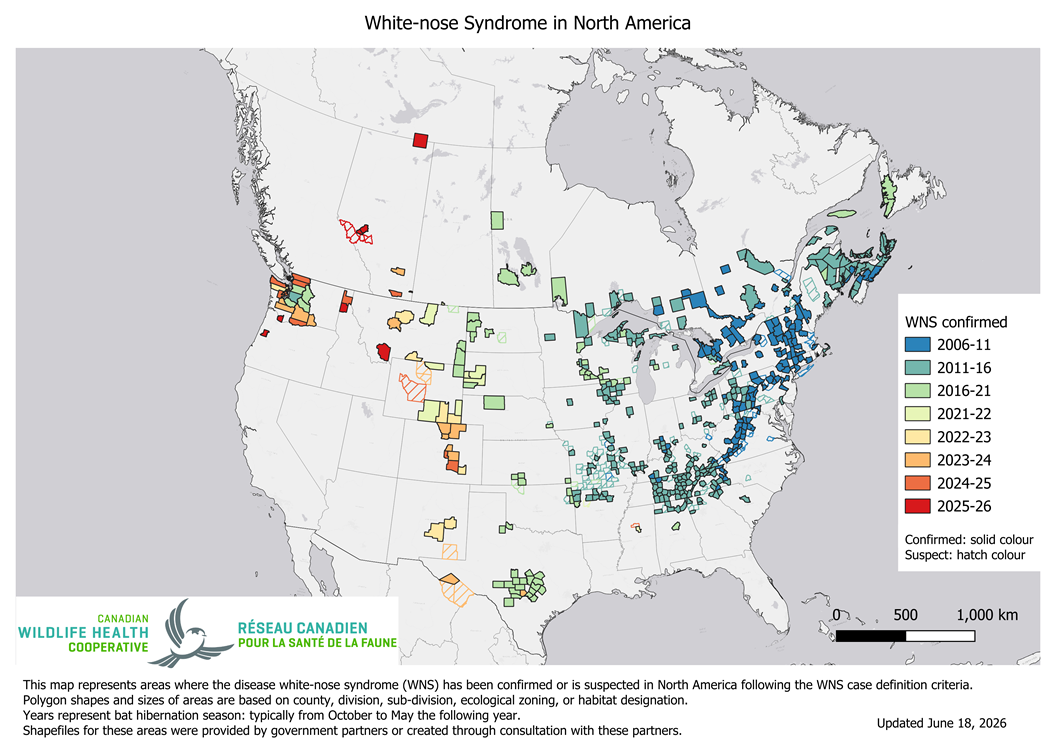
\includegraphics[width=1\linewidth,height=\textheight,keepaspectratio]{Figures/WNS-USandCanada.png}

}

\caption{\label{fig-WNS}White-nose syndrome (WNS) and Pseudogymnoascus
destructans (Pd) occurrence in The US and Canada. Source: CWHC-RCSF
(2026)}

\end{figure}%

\newpage{}

\subsection{Acoustic Monitoring of
Bats}\label{acoustic-monitoring-of-bats}

Acoustic recording is a cost-effective method for monitoring bat
populations across large geographic and temporal scales. However,
several limitations affect the conclusions that can be drawn from these
data and trend estimates cannot be produced for all species using
acoustic methods alone:

\begin{enumerate}
\def\labelenumi{\arabic{enumi}.}
\item
  \textbf{Imperfect species identification} --- Each bat species can
  produce a broad range of echolocation calls, corresponding to
  different flight behaviours and environmental features. Species with
  similar ecology and physiology often produce overlapping calls,
  particularly in areas with high clutter (obstacles), such as forested
  habitats. Although detectors are deployed to maximize recordings of
  diagnostic (typically Search Phase calls), species identifiability
  will always vary depending on the local species assemblage.
\item
  \textbf{Variable detectability} --- Bat species are not equally
  detectable acoustically. Larger, wide-ranging species produce louder
  calls that travel farther, whereas species with quieter calls or
  specialized habitat use may be less reliably recorded.
\item
  \textbf{Data variability} --- Many factors influence recording quality
  and bat activity, including weather, prey abundance and distribution,
  and local habitat. Additionally, stationary detectors may record an
  individual bat multiple times, meaning stationary acoustic data can
  only inform relative activity and occupancy.
\item
  \textbf{Processing limitations} --- Auto-ID software enables efficient
  processing of large datasets, but is known to have high
  misclassification rates for bats. Manual verification generally
  produces more accurate results, but has its own limitations, including
  significantly higher processing time and cost. We use a combination of
  both approaches, as detailed in the
  \hyperref[manual-verification]{Manual Verification} subsection of the
  Methods.
\end{enumerate}

\subsection{Statistical Models}\label{statistical-models}

Bat monitoring data can be analyzed using different statistical
approaches, each with distinct assumptions and outputs. Activity trend
models examine changes in relative acoustic activity over time,
providing a straightforward measure of whether bat detections are
increasing, decreasing, or remaining stable across the monitoring
network.

Dynamic occupancy models take a different approach, estimating the
probability that a species occupies a given site, while explicitly
accounting for imperfect detection. Rather than treating a non-detection
as an absence, these models distinguish between a species being truly
absent versus simply going undetected, an important consideration given
the variable detectability of bats discussed above. They also track
colonization and extinction probabilities across sites over time,
providing insight into range shifts and local population dynamics.

In 2025, both model types were run to examine differences in results and
assess the complementary information each approach provides.

\section{Methods}\label{methods}

\subsection{Data Collection}\label{data-collection}

\subsubsection{Stationary Surveys}\label{stationary-surveys}

Two to four stationary detectors were deployed across at least two
quadrants per grid cell for a minimum of seven nights. Sites were
selected to maximize species detection and recording quality across
different habitat types (see AK report for details). Deployment occurred
between mid-May and mid-July, after bats have emerged from hibernation
but before young bats are volant. Sites and timing should be kept
consistent between years to minimize variability in conditions affecting
bat activity.

\subsubsection{Transect Surveys}\label{transect-surveys}

Where possible, driving transects were conducted following Loeb et al.
(2015). Bats were recorded along the road by driving at
\textasciitilde32km/h with a microphone mounted vertically inside a
magnetic pvc pipe holder on the vehicle's roof. Transects were 30-45 km
long and were surveyed twice during the stationary deployment period
whenever possible.

\subsubsection{Landscape and Weather
Covariates}\label{landscape-and-weather-covariates}

We considered the same covariates for the activity trend models as those
previously established by Rae and Blejwas (2026). Temperature and
relative humidity were recorded in each grid cell using onsite logging
devices where possible; where loggers were unavailable, values were
drawn from the nearest climate station. For sites in British Columbia,
station records were obtained from the Pacific Climate Impacts
Consortium (PCIC) Provincial Climate Data Set (PCDS), which aggregates
and quality-controls observations from multiple provincial and federal
networks. For sites in Southeast Alaska, station records were obtained
using the Meteostat package in Python (Meteostat 2026), which aggregates
weather station records from multiple agencies. Additional weather
covariates drawn from these station records included nightly mean wind
speed (km/h) and nightly precipitation. Degree days above 10°C since
January 1 were calculated from daily temperature records, and nightly
moon illumination (proportion illuminated × proportion of the night the
moon was above the horizon) was calculated for each site-night.

Site-level covariates were derived from GIS (elevation, distance to
water, water body type) or recorded by grid leaders during deployment
(distance to clutter, percent clutter); estimates of percent clutter
were confirmed using site photos. For sites with smaller ponds that did
not appear on the GIS, we used the distance estimate recorded by the
grid leader.

We explored additional factors influencing colonization and extinction
in the dynamic occupancy models. For those models we included distance
to the nearest road, and distance to timber harvest, calculated as the
distance from each survey location to the closest road or harvest
feature. Road and harvest features for British Columbia were derived
from the unpublished Human Footprint Index (HFI) layer currently being
developed by the Geospatial Centre within Biodiversity Pathways. Road
features for Southeast Alaska were taken from the Alaska Department of
Transportation and Public Facilities
(\href{Model\%20covariates\%20for\%20the\%20activity\%20trend\%20models\%20and\%20dynamic\%20occupancy\%20models\%20were\%20based\%20on\%20those\%20established\%20by\%20@rae2024,\%20with\%20additional\%20exploration\%20of\%20factors\%20influencing\%20colonization\%20and\%20extinction\%20in\%20the\%20dynamic\%20occupancy\%20models.\%20For\%20the\%20dynamic\%20occupancy\%20models\%20we\%20included\%20distance\%20to\%20the\%20nearest\%20road,\%20calculated\%20as\%20the\%20distance\%20from\%20each\%20survey\%20location\%20to\%20the\%20closest\%20road\%20feature.\%20Road\%20features\%20for\%20British\%20Columbia\%20were\%20derived\%20from\%20the\%20unpublished\%20Human\%20Footprint\%20Index\%20(HFI)\%20layer\%20currently\%20being\%20developed\%20by\%20the\%20Geospatial\%20Centre\%20within\%20Biodiversity\%20Pathways,\%20while\%20those\%20for\%20Southeast\%20Alaska\%20were\%20taken\%20from\%20the\%20Alaska\%20Department\%20of\%20Transportation\%20and\%20Public\%20Facilities\%20(AKDOT)\%20Roads\%20layer,\%20a\%20statewide\%20road-centerline\%20dataset\%20distributed\%20through\%20the\%20State\%20of\%20Alaska\%20open-data\%20portal\%20(https://gis.data.alaska.gov/datasets/AKDOT::roads-akdot/about).}{AKDOT})
Roads layer and the US Forest Service Transportation layer. Harvest
features for Southeast Alaska were taken from the US Forest Service
Tongass\_National\_Forest\_Past\_Harvest\_from\_CoverType layer.

\subsubsection{Manual Verification}\label{manual-verification}

In 2024 and 2025 acoustic analysis mostly followed the standards set by
WCSC in previous years (Rae and Blejwas 2026). This included running all
files through two automatic classifiers, Kaleidoscope's Bats of North
America 5.4.0 classifier and Sonobat 3.0's southeast Alaska classifier,
to remove files that do not contain bat pulses and giving a preliminary
bat species identification.

Manual vetting largely follows the protocol of Reichert et al. (2018)
and previous analysis standards developed by WCSC (Rae and Blejwas
2026). The key difference in the 2024 and 2025 acoustic analysis
compared to previous years is that not all automatic species
identifications were manually verified. Instead, based on findings from
Stratton et al. (2022) , at least 50\% of recordings were selected for
manual verification.

\emph{Subsetting for manual verification}

Given the project's large scale, manually vetting all recordings is not
feasible long-term. To address this, the NNW Bat Hub, in collaboration
with WCSC and Brian Paterson, developed procedures to ensure that
selecting a subset of recordings for manual review minimizes biases in
analytical results. These standards prioritize the accurate
identification of rare and difficult-to-recognize species to maintain
the integrity of models and analyses.

To ensure data accuracy, manual verification was conducted based on the
number of recordings that received an autoID tag at each site. For sites
with 200 or fewer tagged recordings, all non-noise recordings were
manually reviewed. For sites with more than 200 tagged recordings,
verification depended on the proportion of recordings assigned a species
label. All tags for rare species (comprising ≤10\% of prior years'
identifications) and commonly misidentified species were fully vetted.
Specifically, all Hoary Bat (\emph{Lasiurus cinereus}) and Silver-haired
Bat (\emph{Lasyonicteris noctivagans}) were reviewed due to the frequent
misclassification of noise files that are tagged as these species.
Additionally, recordings of common species were randomly selected for
verification until 50\% of total recordings were reviewed. If fewer than
50\% of recordings had species tags, all classifier-assigned tags were
manually verified, and ``NoID'' recordings were randomly selected until
50\% of all recordings were reviewed.

Manual verification is complicated by the lack of information on species
ranges within Southeast Alaska. We considered all species found in the
region as potential candidates in all grid cells with the exception of
Long-legged and Yuma Myotis. Long-legged Myotis calls are acoustically
similar to those produced by the much more common Little Brown Myotis
and auto ID software frequently misclassifies the calls of these two
species. Unfortunately, although Little Brown Myotis produces diagnostic
calls, Long-legged Myotis does not. Therefore, in grid cells without
independent confirmation of the presence of Long-legged Myotis, we
downgraded all auto IDs of that species to a Little Brown
Myotis/Long-legged Myotis couplet. Where that species has been confirmed
present, we retained the species identification unless diagnostic
characteristics of Little Brown Myotis were present. Calls of California
Myotis also lack diagnostic characteristics and are acoustically similar
to Yuma Myotis. However, to date Yuma Myotis has been documented only in
the southern portion of Southeast Alaska (Olson and Gunderson 2014)and
prior to 2024 we chose to exclude it as a potential species except for
the Ketchikan and Prince of Wales grids. Beginning in 2024, we started
including it in the species set for all grids in order to be able to
detect any expansion of its range within Southeast Alaska.

\subsection{Statistical Analyses}\label{statistical-analyses}

\subsubsection{Activity Trends}\label{activity-trends}

We conducted species-specific trend analyses using negative binomial
GLMM models as described in Rae and Blejwas (2026). We restricted the
analysis to data from 2019 onward, due to the low number of grid cells
that had been sampled in the years prior (2015 and 2017). We further
limited the analysis to grid cells with at least five years of sampling,
since estimating a temporal trend requires enough repeat visits per cell
to distinguish a directional signal from year-to-year variation.

For each species, we performed model selection by fitting the base model
augmented with every combination of up to four covariates, excluding
combinations that would introduce collinearity. This produced 387
candidate models per species, from which we selected the model with the
lowest AIC as the final covariate set Table~\ref{tbl-cov}.

\begin{longtable}[l]{>{\raggedright\arraybackslash}p{15em}>{\raggedright\arraybackslash}p{8em}>{\raggedright\arraybackslash}p{20em}}

\caption{\label{tbl-cov}Top-performing stationary models selected via
AIC-based stepwise selection. Covariates are described as, Distance to
Clutter = distance (m) to nearest object; Percent Clutter = estimated
percentage of space within a 50m radius obstructed by objects; Water
Nearby = detector within 100m of water; WaterDist = distance (m) to
nearest water feature; Nightly Temperature = nightly air temperature
(°C); RH = nightly relative humidity (\%); Nightly Mean Wind Speed =
mean nightly wind speed (m/s); Nightly Precipitation = total nightly
precipitation (mm); jNight = Julian date (day of year) of the survey
night.}

\tabularnewline

\toprule
Species & Species Code & Top Performing Model Covariates\\
\midrule
Hoary Bat & LACI & \\
Silver-haired Bat & LANO & Percent Clutter,Water Nearby,Nightly Min RH\\
California Myotis & MYCA & Percent Clutter,Nightly Precipitation\\
Long-eared Myotis & MYEV & Distance to Clutter  m ,Nightly Max Temperature,Nightly Min RH,jNight\\
Little Brown Myotis & MYLU & Percent Clutter,WaterDist,Nightly Precipitation,Nightly Mean Wind Speed\\
\addlinespace
Long-legged Myotis & MYVO & \\
Yuma Myotis & MYYU & \\
\bottomrule

\end{longtable}

Post-hoc tests were run on the final models to ensure proper model fit.
Species were excluded from the analysis if model fit was not appropriate
due to issues including under-dispersion or standard errors that were
more than 3 times the estimate. Model results were also excluded if
there was less than 150 recordings across all sample years.

\paragraph{Use of Automated Identification Results in Stationary Trend
Analyses}\label{use-of-automated-identification-results-in-stationary-trend-analyses}

For stationary trend analyses, species identifications came from the
Kaelidoscope Pro AutoID software, not from manual verification. Manual
review was used only to remove non-bat noise. Specifically, files that
manual review flagged as noise were excluded, but where manual review
suggested a different species than the AutoID label, the AutoID
classification was retained.

This approach was first identified as necessary in 2023 (Rae and Lausen
2024), when analyses of manually verified data revealed a consistent
positive trend across all species, this was interpreted as an artifact
of reviewer learning over time rather than a true biological signal. As
verifier experience increased across years, calls were increasingly
assigned to specific species rather than left unidentified, producing an
apparent increase in detections independent of actual bat activity.
Because this observer effect is difficult to control for statistically,
AutoID classifications are now used as the standard for all activity
trend analyses, as automated classifiers apply consistent criteria
across all years. While AutoID is subject to some misclassification, the
error rate is consistent across years and does not confound detection of
genuine temporal trends.

Trend analyses are presented only for species confirmed present through
manual verification and for which models fully converged.

\subsubsection{Transect Abundance
Models}\label{transect-abundance-models}

For the transect-based abundance trend models, we used only manually
verified detections. When a detection was flagged as a species couplet,
it was counted toward each species in the couplet. As above, we
restricted the data to transect surveys from 2019 onward and to grid
cells with at least five years of sampling. Covariates were limited to
weather variables and transect length, and candidate models excluded any
combination of collinear variables. We fit 59 candidate models per
species and selected the one with the lowest AIC as the final covariate
set Table~\ref{tbl-cov-transects}.

\begin{longtable}[l]{>{\raggedright\arraybackslash}p{15em}>{\raggedright\arraybackslash}p{8em}>{\raggedright\arraybackslash}p{20em}}

\caption{\label{tbl-cov-transects}Top-performing transect models
selected via AIC-based stepwise selection.}

\tabularnewline

\toprule
Species & Species Code & Top Performing Model Covariates\\
\midrule
Hoary Bat & LACI & \\
Silver-haired Bat & LANO & Nightly Min Temperature,Nightly Max RH\\
California Myotis & MYCA & \\
Long-eared Myotis & MYEV & \\
Little Brown Myotis & MYLU & Nightly Max RH,Nightly Mean Wind Speed\\
\addlinespace
Long-legged Myotis & MYVO & \\
Yuma Myotis & MYYU & \\
\bottomrule

\end{longtable}

After selection, we ran a series of post-hoc checks to confirm model
fit. We treated a species' result as reliable only when these tests
agreed that the year effect reflected a genuine regional trend rather
than an artefact of sparse counts or a single influential cell.

\subsubsection{Dynamic Occupancy}\label{dynamic-occupancy}

We fitted multi-season (dynamic) occupancy models (MacKenzie et al.
2003) to estimate trends in occupancy, colonization, and persistence
while accounting for imperfect detection. This analysis used nightly
acoustic detection/non-detection data from passive bat detectors
deployed at 43 stationary detector sites located in 9 grid cells in
Southeast Alaska, as well as 173 stationary detector sites in 56 grid
cells in British Columbia (BC). Pooling the two regions allowed the more
extensive BC data to inform species-specific detection probabilities and
covariate slopes, improving our ability to distinguish true absences
from non-detections and thereby sharpening occupancy estimates where
Alaska data were sparse. A region effect accounted for structural
differences in the landscape between British Columbia and southeast
Alaska, allowing us to characterize occupancy trends for southeast
Alaska with greater precision than an Alaska-only model would permit.

Data were filtered to the 2017--2025 period, and analysis used an
every-other-night subsampling protocol to reduce temporal
autocorrelation between consecutive nights, using a maximum of 4 nights
per site-year. Sites had to have a minimum of 2 nights of data within a
given year and data from at least 2 years total. Models were run
separately for all 7 bat species.

Initial occupancy (\(\psi\)) was modeled as a function of elevation and
water nearby, with a random effect for region. Baseline occupancy for
the Alaska region was estimated from Alaska detections only and was not
forced toward the BC average. Colonization (\(\gamma\)) and persistence
(\(\varphi\)) were modeled with time-varying intercepts and distance to
road as a covariate. Detection probability (p) was modeled as a function
of percent clutter, nightly mean temperature, and Julian night.

All continuous covariates were standardized by centering on their mean
and dividing by their standard deviation; missing covariate values were
imputed with the global mean prior to standardization.

Models were fit in a Bayesian framework using JAGS (Version 4.3.2) via
the \texttt{jagsUI} package (Version 1.6.3) in r (Version 4.5.1). We ran
3 chains in parallel for 30,000 iterations each, discarding the first
15,000 as burn-in and thinning the remainder by 5, yielding 9,000
posterior samples for inference. Priors on all regression coefficients
were normal with mean 0 and precision 0.368 (equivalent to a standard
deviation of approximately 1.65), and the standard deviation of the
region-level random effect was assigned a Uniform(0, 5) prior.
Convergence was assessed using Rhat diagnostics, with values below 1.1
taken to indicate convergence. Results are summarized using posterior
means and 95\% Bayesian credible intervals. We calculated an overall
occupancy trend metric (𝜆) as the ratio of estimated occupancy in the
final year to that in the initial year; values of 𝜆 \textgreater{} 1
with 95\% credible intervals entirely above 1 indicate an increase in
occupancy, values 𝜆\textless1 with intervals entirely below 1 indicate a
decline, and intervals overlapping 1 indicate an uncertain or stable.

\section{Results}\label{results}

In 2024 all 9 grid cells were monitored, and in 2025 a total of 6 grid
sites were sampled in SE Alaska and 3 newly established sites were
sampled in the Anchorage area (Figure~\ref{fig-sites}).

\begin{figure}[H]

\centering{

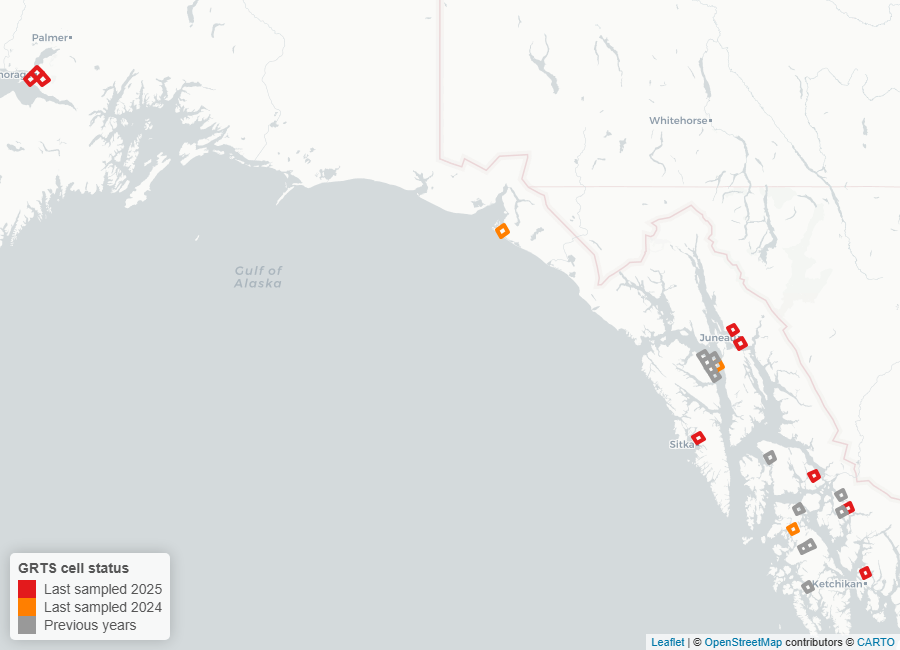
\includegraphics[width=1\linewidth,height=\textheight,keepaspectratio]{Figures/site_summary_map.png}

}

\caption{\label{fig-sites}Acoustic bat monitoring sites in Alaska in
2025.NABat grid cells monitored (with two or more stationary sites) in
2025 appear in red and those monitored in 2024 in orange. Cells
monitored in previous years but not in 2024 or 2025 appear in grey.}

\end{figure}%

\subsection{Activity Summary and
Trends}\label{activity-summary-and-trends}

Total acoustic activity varied substantially across sites and years,
with Little Brown Myotis dominating call volume at every site in nearly
every year. Overall detection totals were highest at the northern sites:
Yakutat produced the single largest site-year total
(\textasciitilde17,500 calls in 2024), and Juneau recorded consistently
high volumes (\textasciitilde12,000 in 2020 and \textasciitilde13,500 in
2024). Southern and central sites generally recorded lower totals, with
Petersburg (\textasciitilde9,000 in 2024) and POW (\textasciitilde7,500
in 2024) reaching comparable peaks in single years, while Wrangell and
Hoonah remained low throughout (generally under \textasciitilde2,000
calls per year). Most sites recorded substantially higher activity in
2024 than in any other year.

\begin{figure}[H]

\centering{

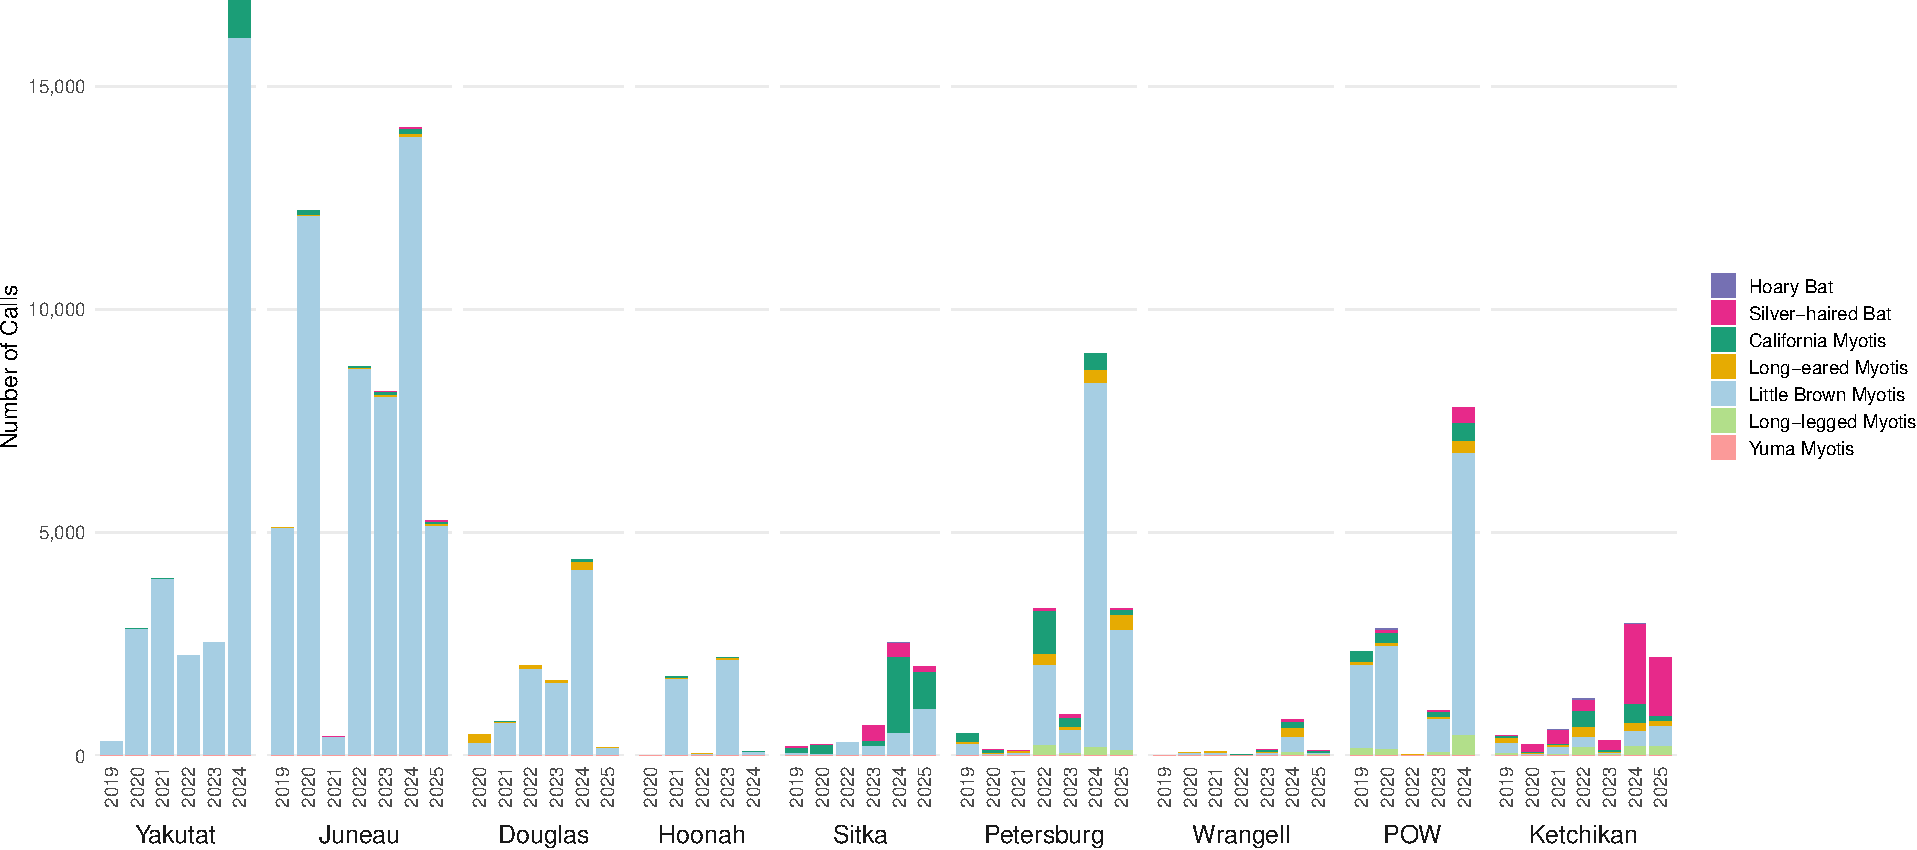
\includegraphics[width=1\linewidth,height=\textheight,keepaspectratio]{NABat-AK_files/figure-pdf/fig-activitysummary-1.pdf}

}

\caption{\label{fig-activitysummary}Relative activity of bat species
detected during NABat monitoring in 9 grid cells in Southeast Alaska,
arranged north to south, during 2019-2025}

\end{figure}%

We estimated yearly trends in nightly acoustic activity for seven
species across the stationary detector and mobile transect survey
streams. Five species produced reportable stationary-detector models;
two (Long-legged Myotis, Yuma Myotis) could not be reliably fit and are
not reported Table~\ref{tbl-models}. For transect abundance trends we
only report on the results of Silver-haired bat and Little Brown bat
since these were the only two species were modelling results were
reliable.

Silver-haired Bat showed the clearest and most consistent signal, with
activity increasing significantly over the monitoring period in both the
stationary (β = 0.48 ± 0.17, p \textless{} 0.001) and transect (β = 0.40
± 0.20, p = 0.001) datasets, the only species for which a significant
trend was recovered independently in both survey types.

California Myotis showed an increase in activity from the stationary
model (β = 0.14 ± 0.13, p = 0.036). Long-eared Myotis (β = 0.06 ± 0.13,
p = 0.35) and Little Brown Myotis (stationary β = 0.08 ± 0.14, p = 0.24;
transect β = 0.00 ± 0.12, p = 0.94) showed no detectable trend, with
confidence intervals spanning zero in both reportable models.

Hoary Bat, Long-legged Myotis and Yuma Myotis are not reported: Hoary
bat and Long-legged Myotis fell below the detection threshold required
for trend estimation, and the Yuma Myotis model failed to converge.

\begin{table}[H]

\caption{\label{tbl-models}Trend estimates from NABat stationary and
transect monitoring in southeast Alaska, 2019--2025, adjusted for
covariates. Estimates are on the natural-log scale. Stationary and
transect models were fit separately as independent pipelines; blank
cells indicate species that did not meet the criteria for reporting in
that framework. Significant results (p \textless{} 0.05) are shown in
bold.}

\centering{

\centering
\begin{tabular}{l>{}r>{}r>{}r>{}r}
\toprule
\multicolumn{1}{c}{ } & \multicolumn{2}{c}{Stationary Models} & \multicolumn{2}{c}{Transect Models} \\
\cmidrule(l{3pt}r{3pt}){2-3} \cmidrule(l{3pt}r{3pt}){4-5}
Species & Trend Estimate ± 95\%CI & P-value & Trend Estimate ± 95\%CI & P-value\\
\midrule
Hoary Bat &  &  &  & \\
Silver-haired Bat & \textbf{0.48 ± 0.17} & \textbf{<0.001} & \textbf{0.40 ± 0.20} & \textbf{<0.001}\\
California Myotis & \textbf{0.14 ± 0.13} & \textbf{0.036} &  & \\
Long-eared Myotis & 0.06 ± 0.13 & 0.352 &  & \\
Little Brown Myotis & 0.08 ± 0.14 & 0.242 & 0.00 ± 0.12 & 0.937\\
\addlinespace
Long-legged Myotis &  &  &  & \\
Yuma Myotis &  &  &  & \\
\bottomrule
\end{tabular}

}

\end{table}%

\subsection{Dynamic Occupancy}\label{dynamic-occupancy-1}

Dynamic occupancy models converged for all species. Due to the low
number of Hoary bat detections across the monitoring period all Hoary
bat results were removed from this report. Four species showed
increasing occupancy over the 2017--2025 period, comprising all Myotis
species except California Myotis: Long-legged Myotis (λ = 1.43, 95\% CI
1.18--1.77), Long-eared Myotis (λ = 1.25, 1.05--1.50), Little Brown
Myotis (λ = 1.10, 1.03--1.19), and Yuma Myotis (λ = 1.44, 1.17--1.79)
Table~\ref{tbl-occ-trends}.

For the remaining three species, Silver-haired Bat (λ = 1.05,
0.95--1.17), and California Myotis (λ = 1.16, 1.00--1.35), the 95\%
credible interval for λ overlapped 1, indicating that no directional
change in occupancy could be detected.

\begin{table}

\caption{\label{tbl-occ-trends}Occupancy trend estimates from the
dynamic occupancy models (pooled British Columbia and Southeast Alaska),
2017--2025. The trend slope is the per-year change in occupancy on the
model scale; \(\lambda\) is the ratio of occupancy in the final year
(2025) to the initial year (2017). Values are posterior means with 95\%
credible intervals. A \(\lambda\) interval entirely above 1 indicates
increasing occupancy; an interval overlapping 1 indicates no directional
change could be detected.}

\centering{

\centering
\begin{tabular}[t]{llc}
\toprule
Species & Trend slope (95% CI) & $\lambda$ (95% CI)\\
\midrule
Hoary Bat &  & \\
Silver-haired Bat & 0.0085 (0.0009, 0.0160) & 1.05 (0.95, 1.17)\\
California Myotis & 0.0158 (0.0069, 0.0250) & 1.16 (1.00, 1.35)\\
\textbf{Long-eared Myotis} & 0.0276 (0.0174, 0.0381) & 1.25 (1.05, 1.50)\\
\textbf{Little Brown Myotis} & 0.0142 (0.0090, 0.0200) & 1.10 (1.03, 1.19)\\
\addlinespace
\textbf{Long-legged Myotis} & 0.0246 (0.0144, 0.0346) & 1.43 (1.18, 1.77)\\
\textbf{Yuma Myotis} & 0.0151 (0.0065, 0.0233) & 1.44 (1.17, 1.79)\\
\bottomrule
\end{tabular}

}

\end{table}%

Covariate effects varied by species, but temperature was the most
consistent detection covariate, with warmer nights associated with
higher detection probability for most species. Clutter effects on
detection probability were present but species-specific, and Julian date
effects were mixed across speciesTable~\ref{tbl-occ-covariates}.

\begin{table}

\caption{\label{tbl-occ-covariates}Covariate effects from the dynamic
occupancy models (pooled British Columbia and Southeast Alaska), on the
standardized model scale. Each cell gives the posterior mean and 95\%
credible interval; only effects whose interval excludes zero are shown,
and a dash indicates the covariate was included but its 95\% credible
interval overlapped zero. \(\psi\) = initial occupancy, \(\gamma\) =
colonization, \(\varphi\) = persistence, \(p\) = detection.}

\centering{

\centering\begingroup\fontsize{8}{10}\selectfont

\begin{tabular}[t]{lccccccc}
\toprule
\multicolumn{1}{c}{ } & \multicolumn{7}{c}{Species} \\
\cmidrule(l{3pt}r{3pt}){2-8}
Covariate & LACI & LANO & MYCA & MYEV & MYLU & MYVO & MYYU\\
\midrule
\addlinespace[0.3em]
\multicolumn{8}{l}{\textbf{Initial occupancy ($\psi$)}}\\
\hspace{1em}Elevation &  & — & -0.91 (-1.76, -0.16) & — & — & — & -1.83 (-2.81, -0.95)\\
\hspace{1em}Water nearby &  & — & 1.79 (0.49, 3.36) & — & — & — & —\\
\addlinespace[0.3em]
\multicolumn{8}{l}{\textbf{Colonization ($\gamma$)}}\\
\hspace{1em}Distance to road &  & -0.49 (-0.91, -0.16) & — & — & — & -0.61 (-1.35, -0.18) & —\\
\addlinespace[0.3em]
\multicolumn{8}{l}{\textbf{Persistence ($\varphi$)}}\\
\hspace{1em}Distance to road &  & -0.42 (-0.73, -0.07) & — & — & — & — & -0.78 (-1.40, -0.13)\\
\addlinespace[0.3em]
\multicolumn{8}{l}{\textbf{Detection ($p$)}}\\
\hspace{1em}Percent clutter &  & — & 0.22 (0.13, 0.32) & 0.11 (0.02, 0.19) & — & 0.16 (0.08, 0.25) & —\\
\hspace{1em}Nightly temperature &  & 0.47 (0.36, 0.57) & 0.23 (0.14, 0.33) & — & 0.24 (0.14, 0.34) & 0.15 (0.06, 0.24) & —\\
\hspace{1em}Julian night &  & 0.18 (0.09, 0.27) & -0.20 (-0.29, -0.12) & — & 0.28 (0.19, 0.38) & 0.13 (0.05, 0.22) & 0.11 (0.01, 0.22)\\
\bottomrule
\end{tabular}
\endgroup{}

}

\end{table}%

More detailed species results can be found on
\hyperref[sec-appendix-a]{Appendix A}.

\section{Discussion}\label{discussion}

Need to talk about the spike in 2024 data. I looked through the data and
there isn't an issue with duplicate sites. Need to confirm if the sites
were sampled for longer than normal as this might explain the issue
(will need to reference new table that includes deployment sated for
2024 and 2025).

Talk about the differences in results between activity and occupancy
trends. Occupancy trends need a larger change to be detectable, so it
can take a bit longer to be able to detect changes in populations.
Activity metrics are way more noisy so they might show changes quicker
but might not be as reliable and need to have consistent trends over
many years of modelling to say anythign about them.

The reduced survey effort in 2025 was the result of staffing cuts by the
US Forest Service and staffing levels are unlikely to improve in the
near future. Given the already low number of grids currently being
monitored in Southeast Alaska, efforts should be made to find other
agencies or organizations to continue the monitoring in those grids or
to establish new ones.\\
-Also, are there ways to reduce the time it takes to monitor a grid?
Eliminate driving surveys, stop collecting onsite weather data, etc.
that wouldn't impact the analyses?\\
Many more species are present in BC than in SEAK and its possible that
new species may expand their ranges into or within SEAK (MYYU). Is it
feasible to look for species such as EPFU somehow? Maybe run the files
with all the BC species that have diagnostic calls and manually review
any recordings that are identified as one of those species? Not sure if
there are diagnostic characteristics for EPFU like there are for LANO
though.

Main questii: what do we need to change to improve the power of these
analyses. REcommnedations to improve stats)

\section{Appendix A}\label{sec-appendix-a}

\subsection{\texorpdfstring{Hoary Bat (\emph{Lasiurus
cinereus})}{Hoary Bat (Lasiurus cinereus)}}\label{hoary-bat-lasiurus-cinereus}

\pandocbounded{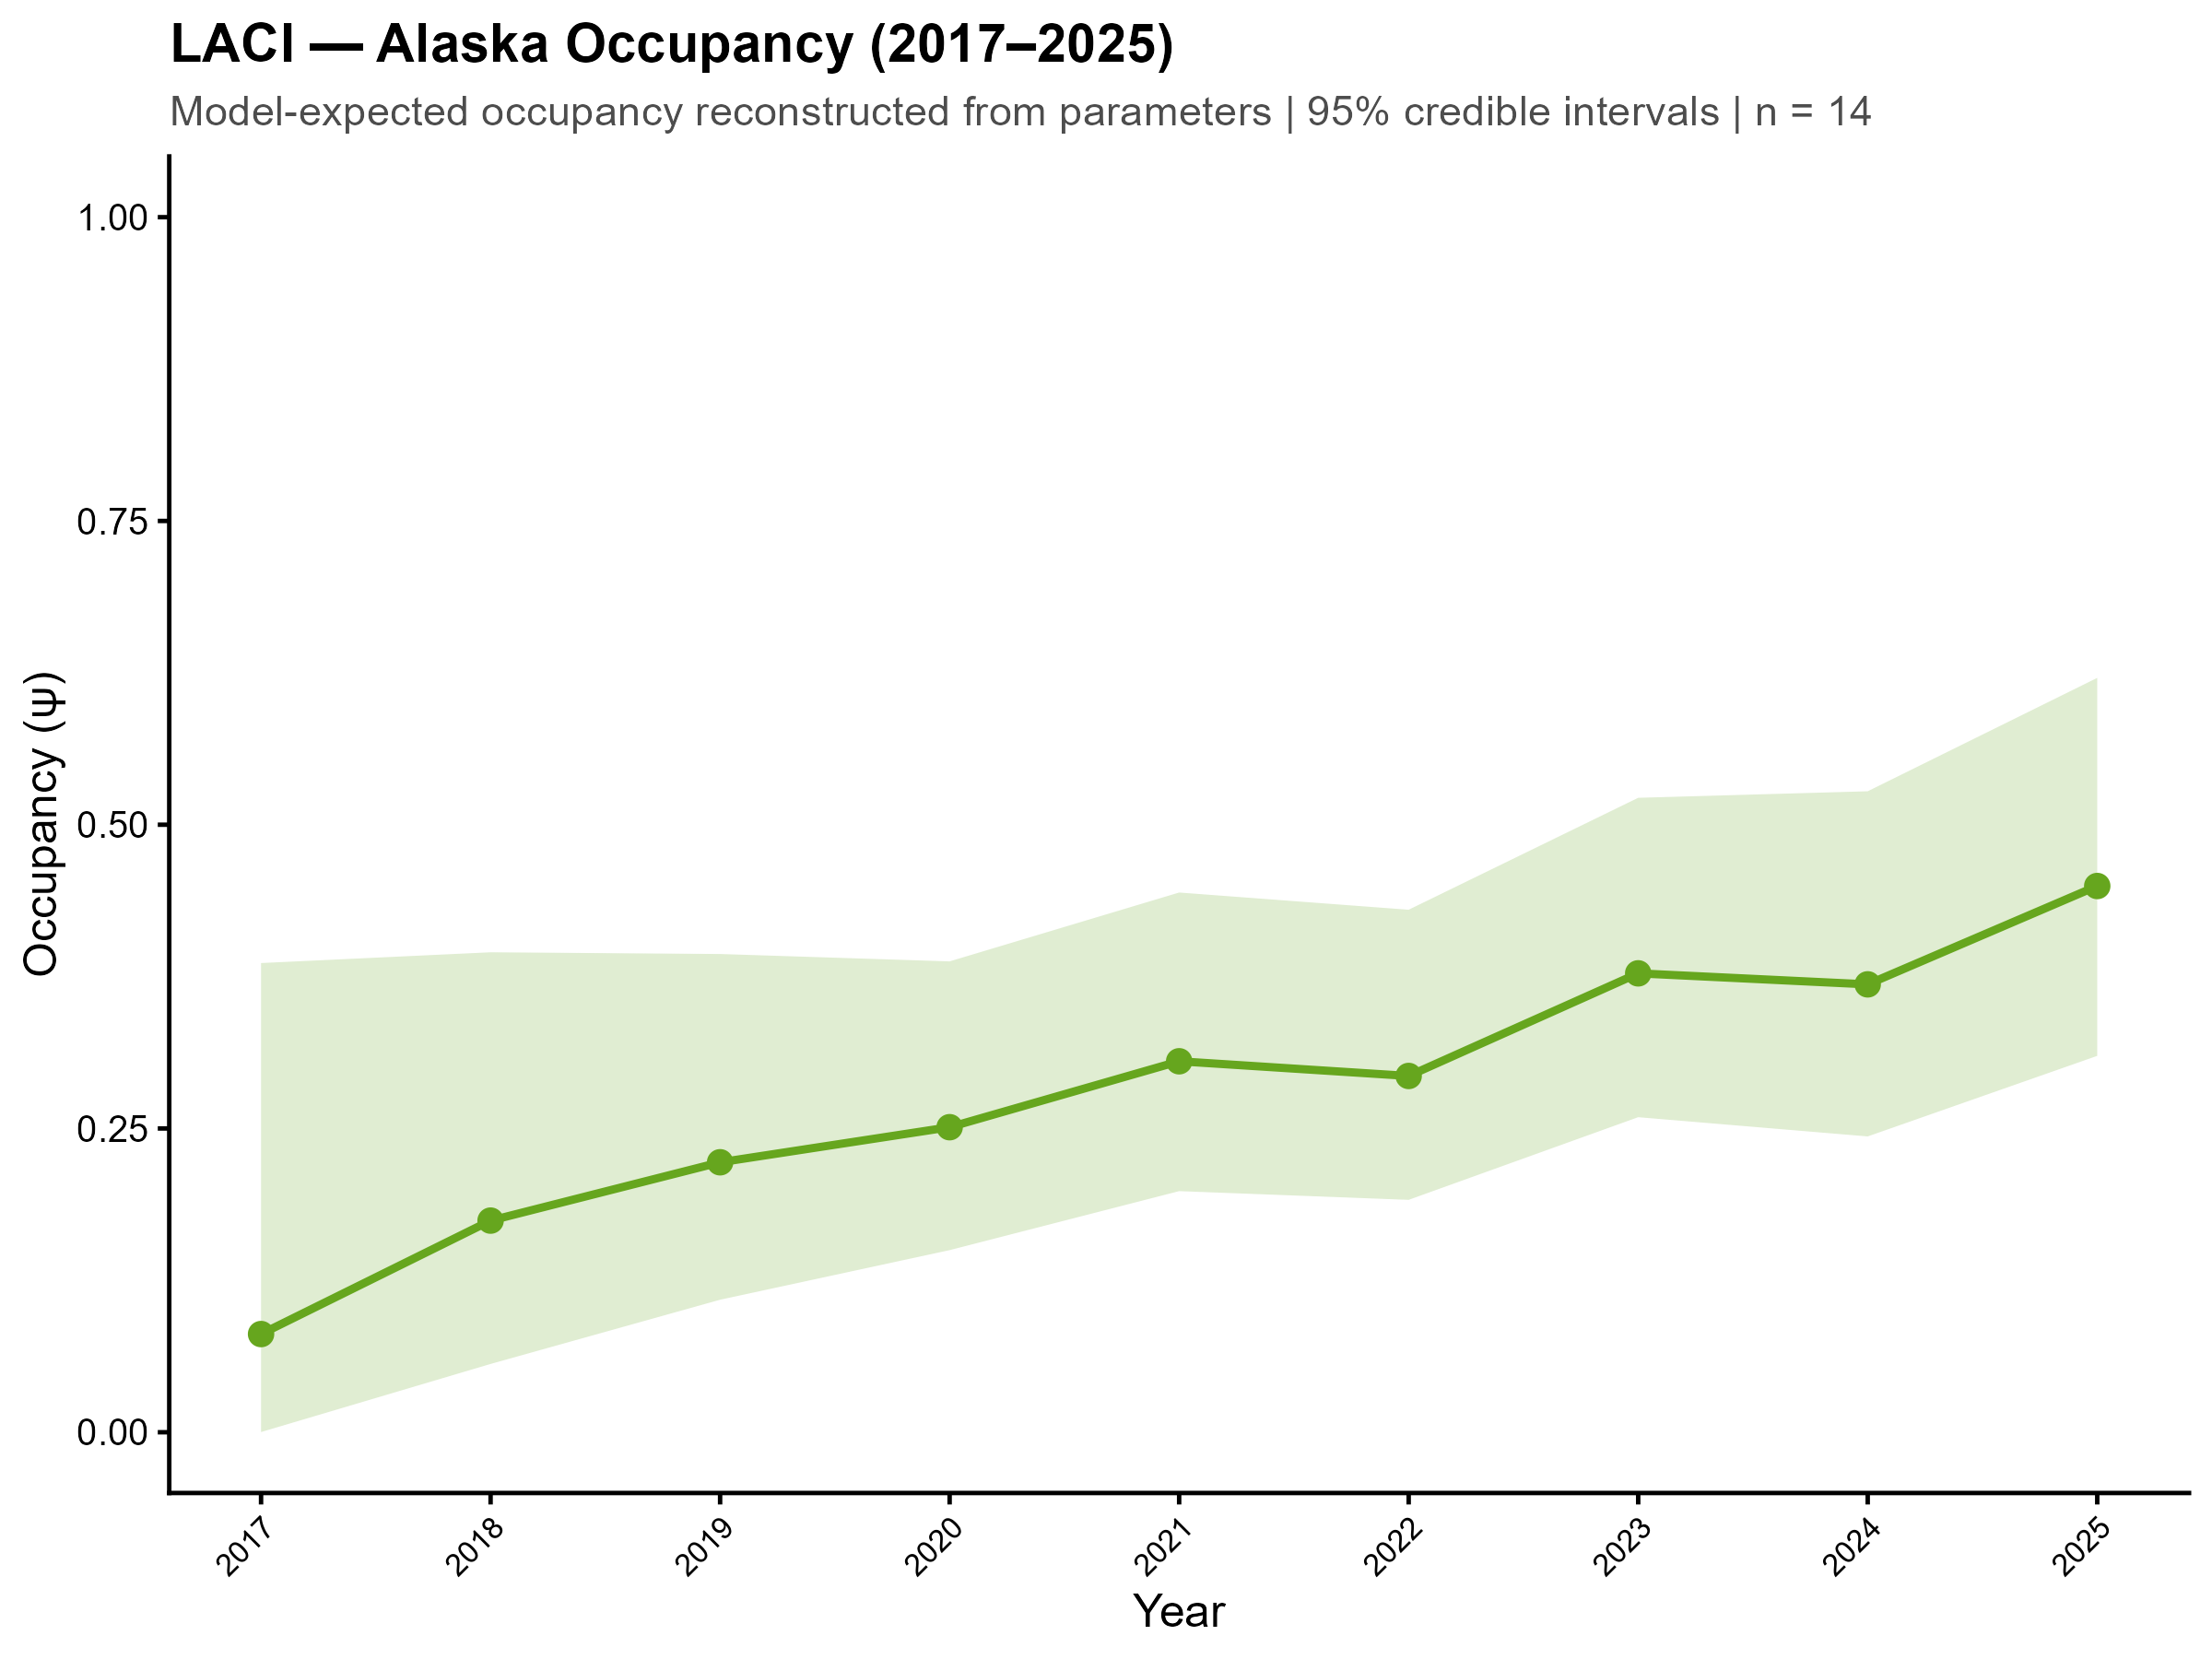
\includegraphics[keepaspectratio]{images/clipboard-1678851271.png}}
\pandocbounded{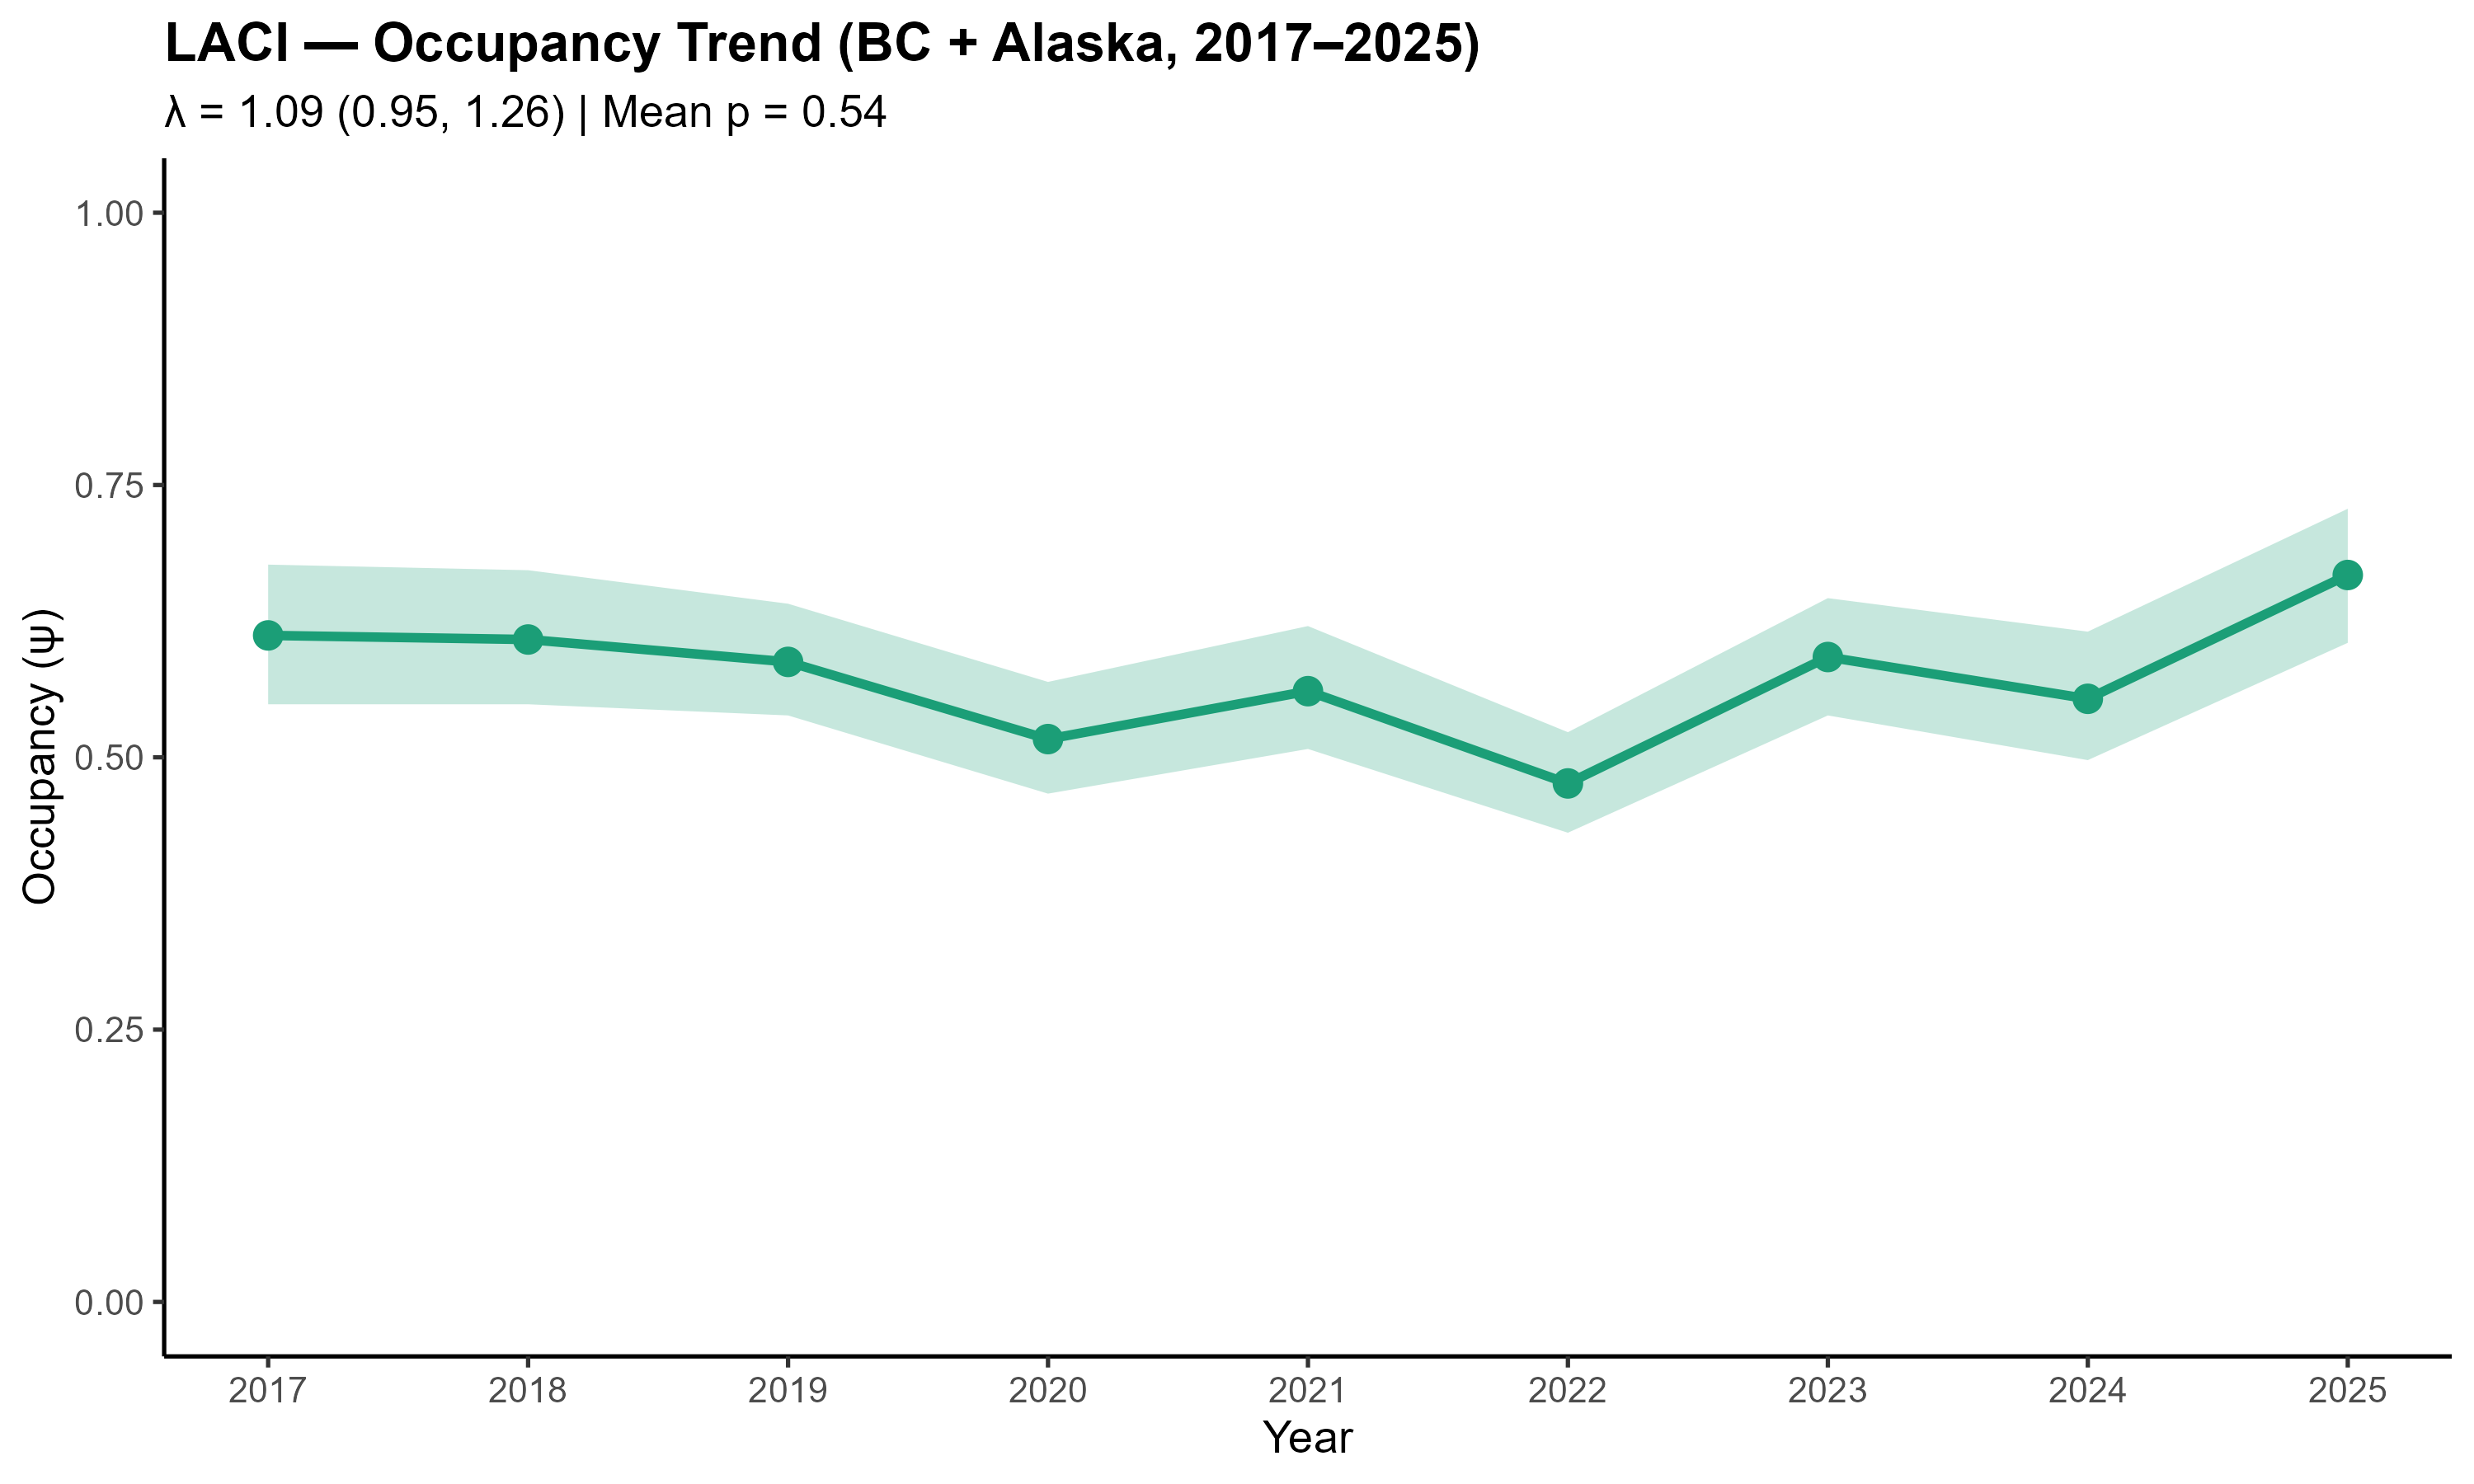
\includegraphics[keepaspectratio]{images/clipboard-2604002813.png}}
\pandocbounded{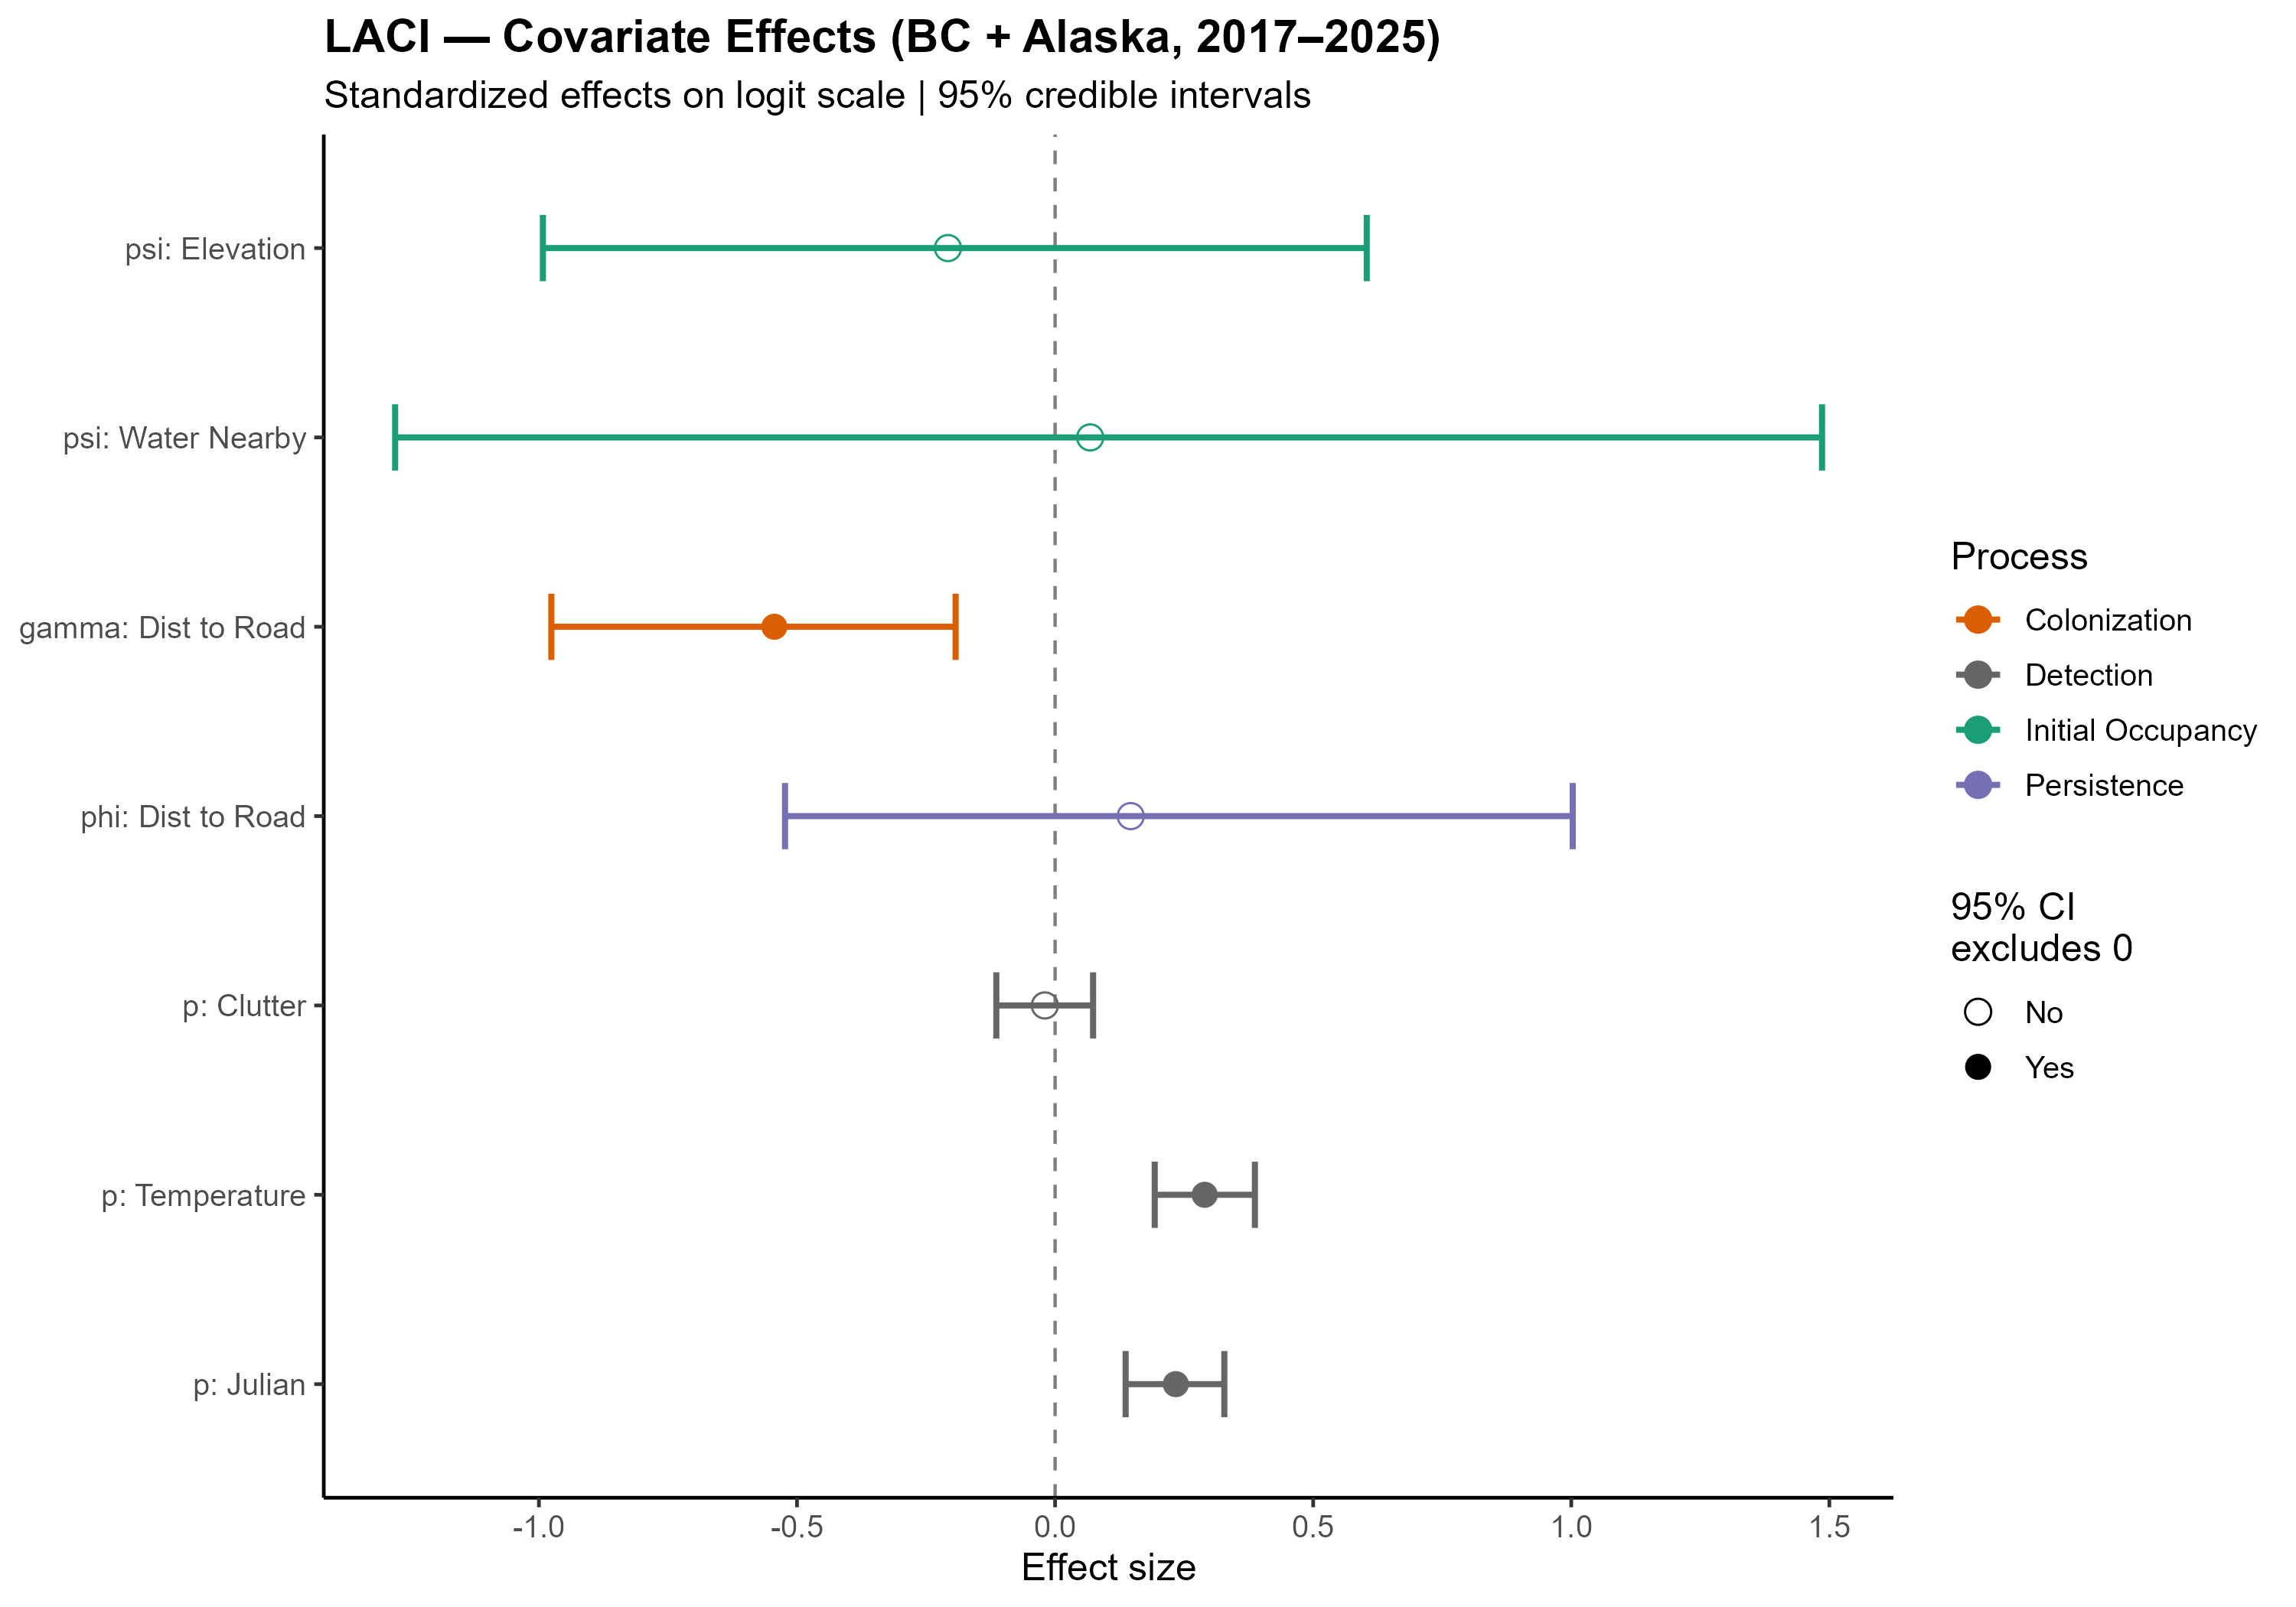
\includegraphics[keepaspectratio]{images/clipboard-539850997.png}}
\pandocbounded{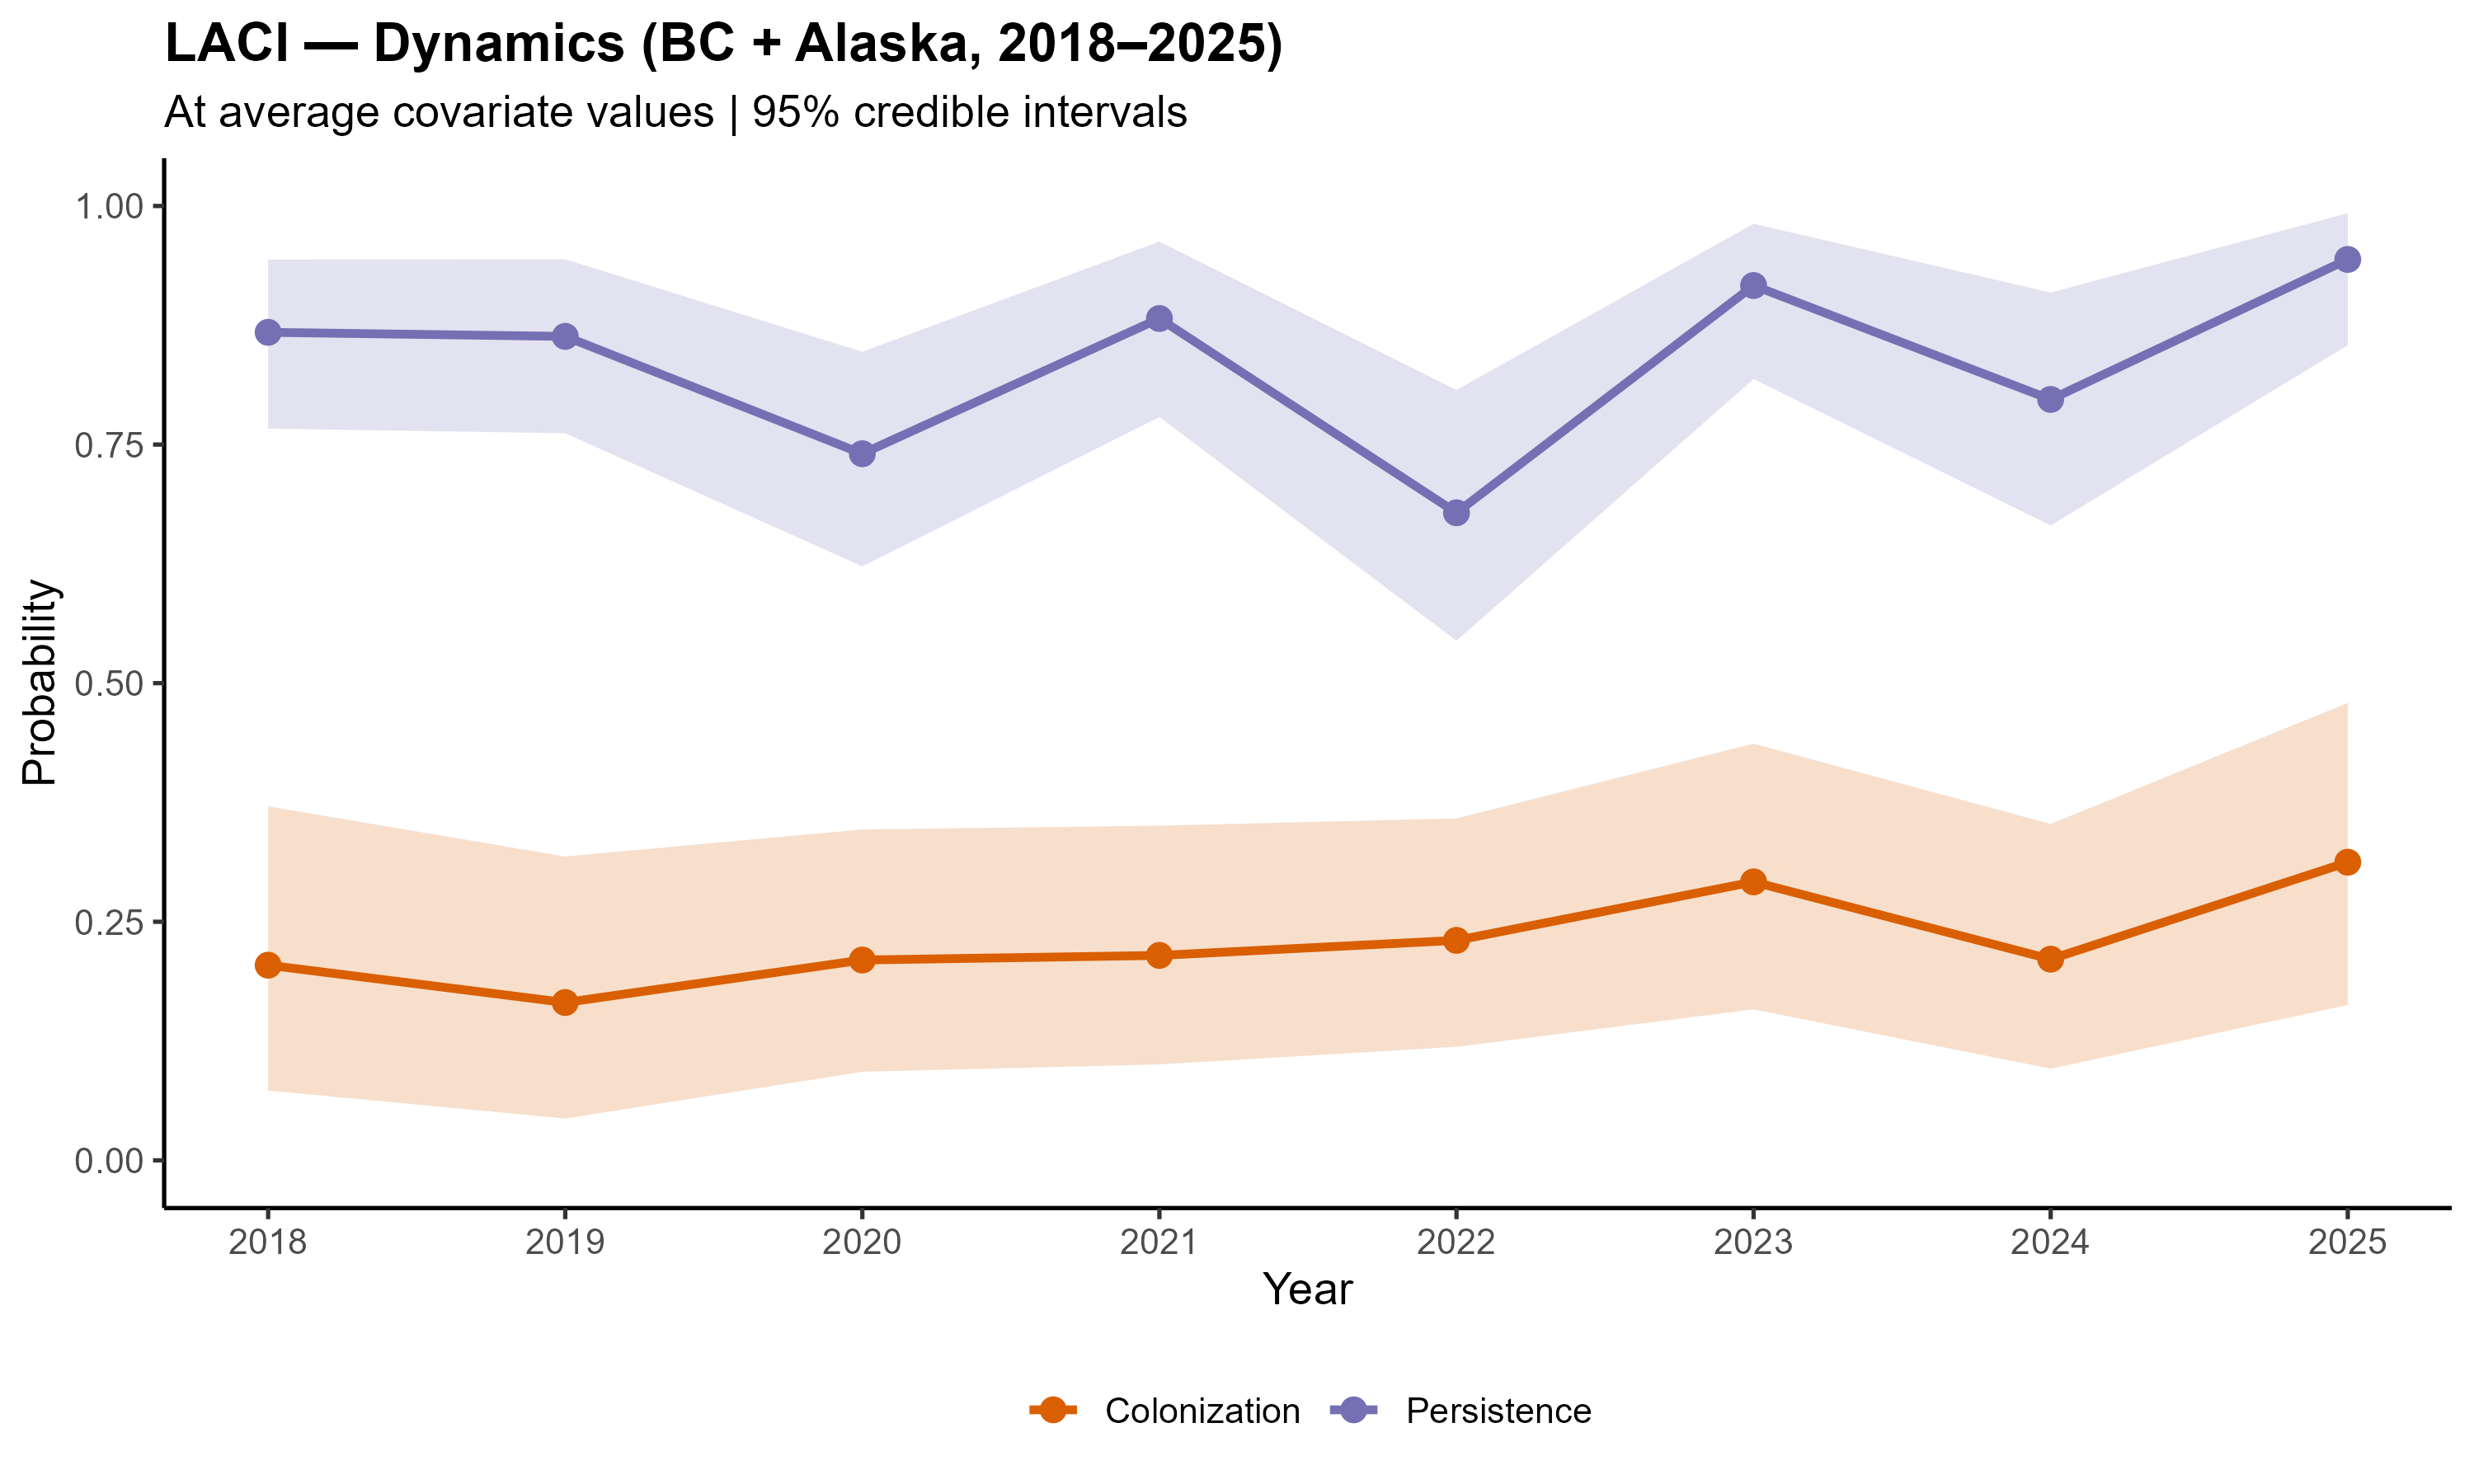
\includegraphics[keepaspectratio]{images/clipboard-4068991790.png}}

\subsection{\texorpdfstring{Silver-haired Bat (\emph{Lasyonicteris
noctivagans})}{Silver-haired Bat (Lasyonicteris noctivagans)}}\label{silver-haired-bat-lasyonicteris-noctivagans}

\pandocbounded{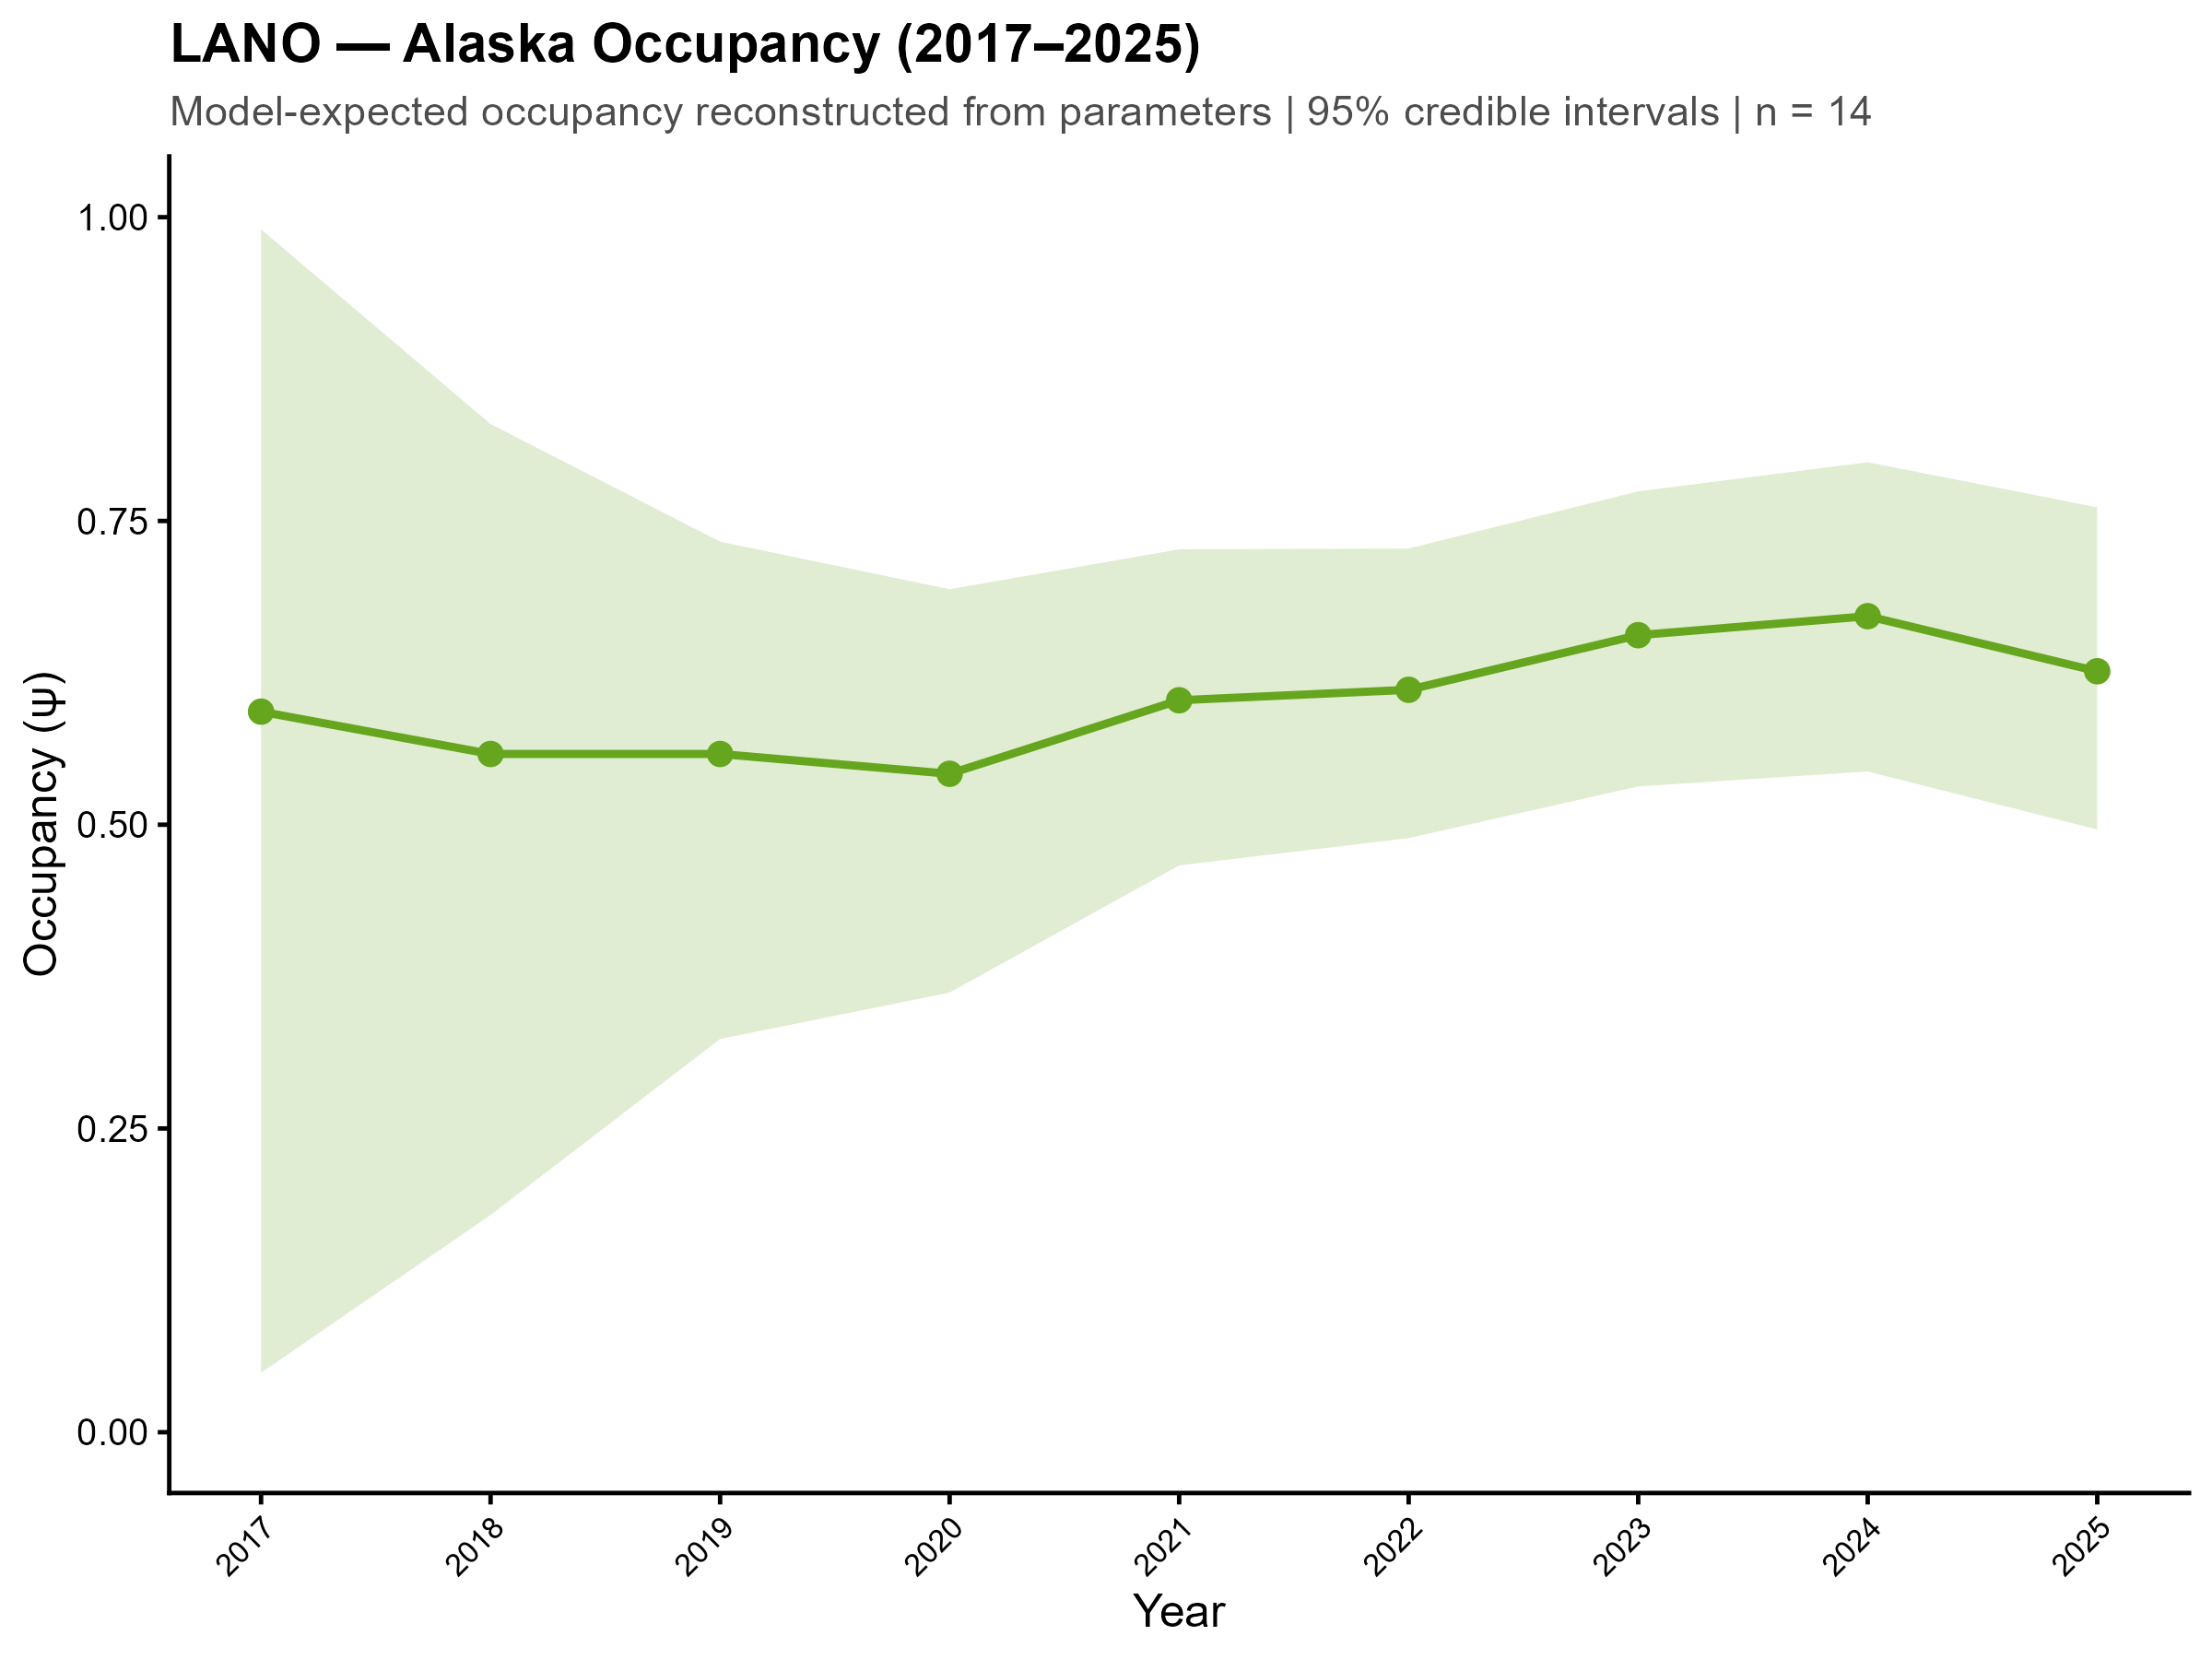
\includegraphics[keepaspectratio]{images/clipboard-3190713865.png}}
\pandocbounded{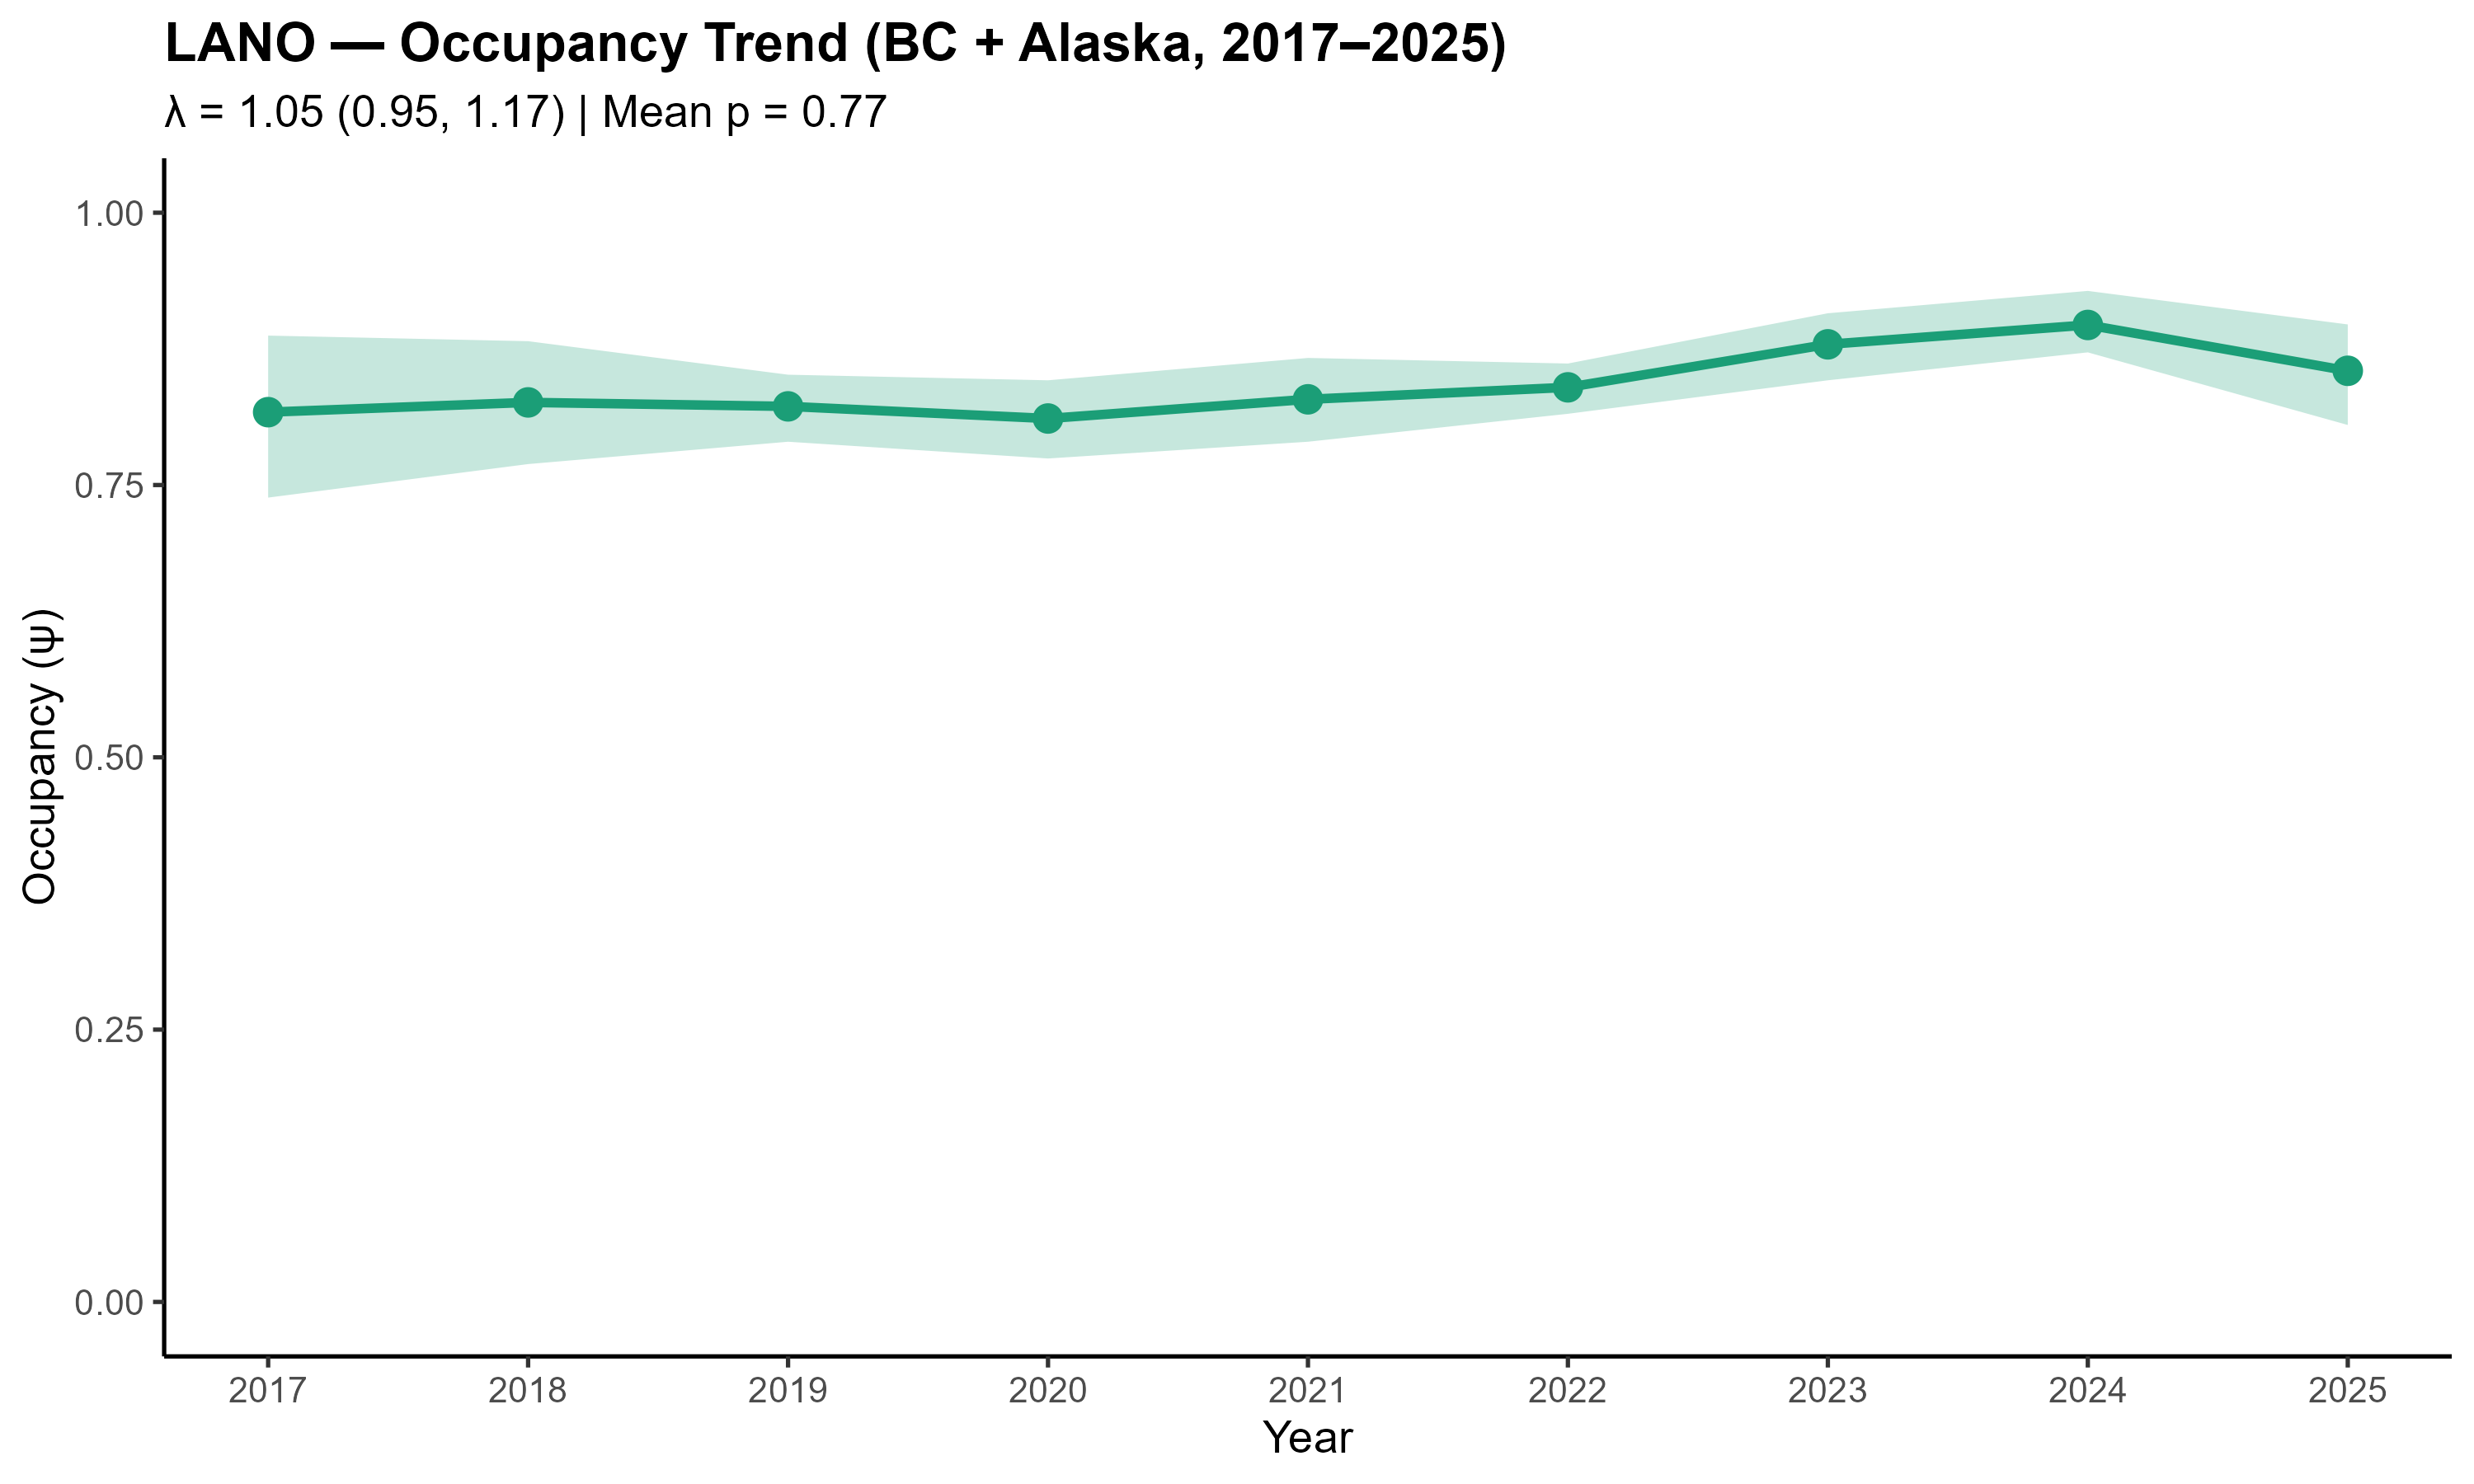
\includegraphics[keepaspectratio]{images/clipboard-2878420209.png}}
\pandocbounded{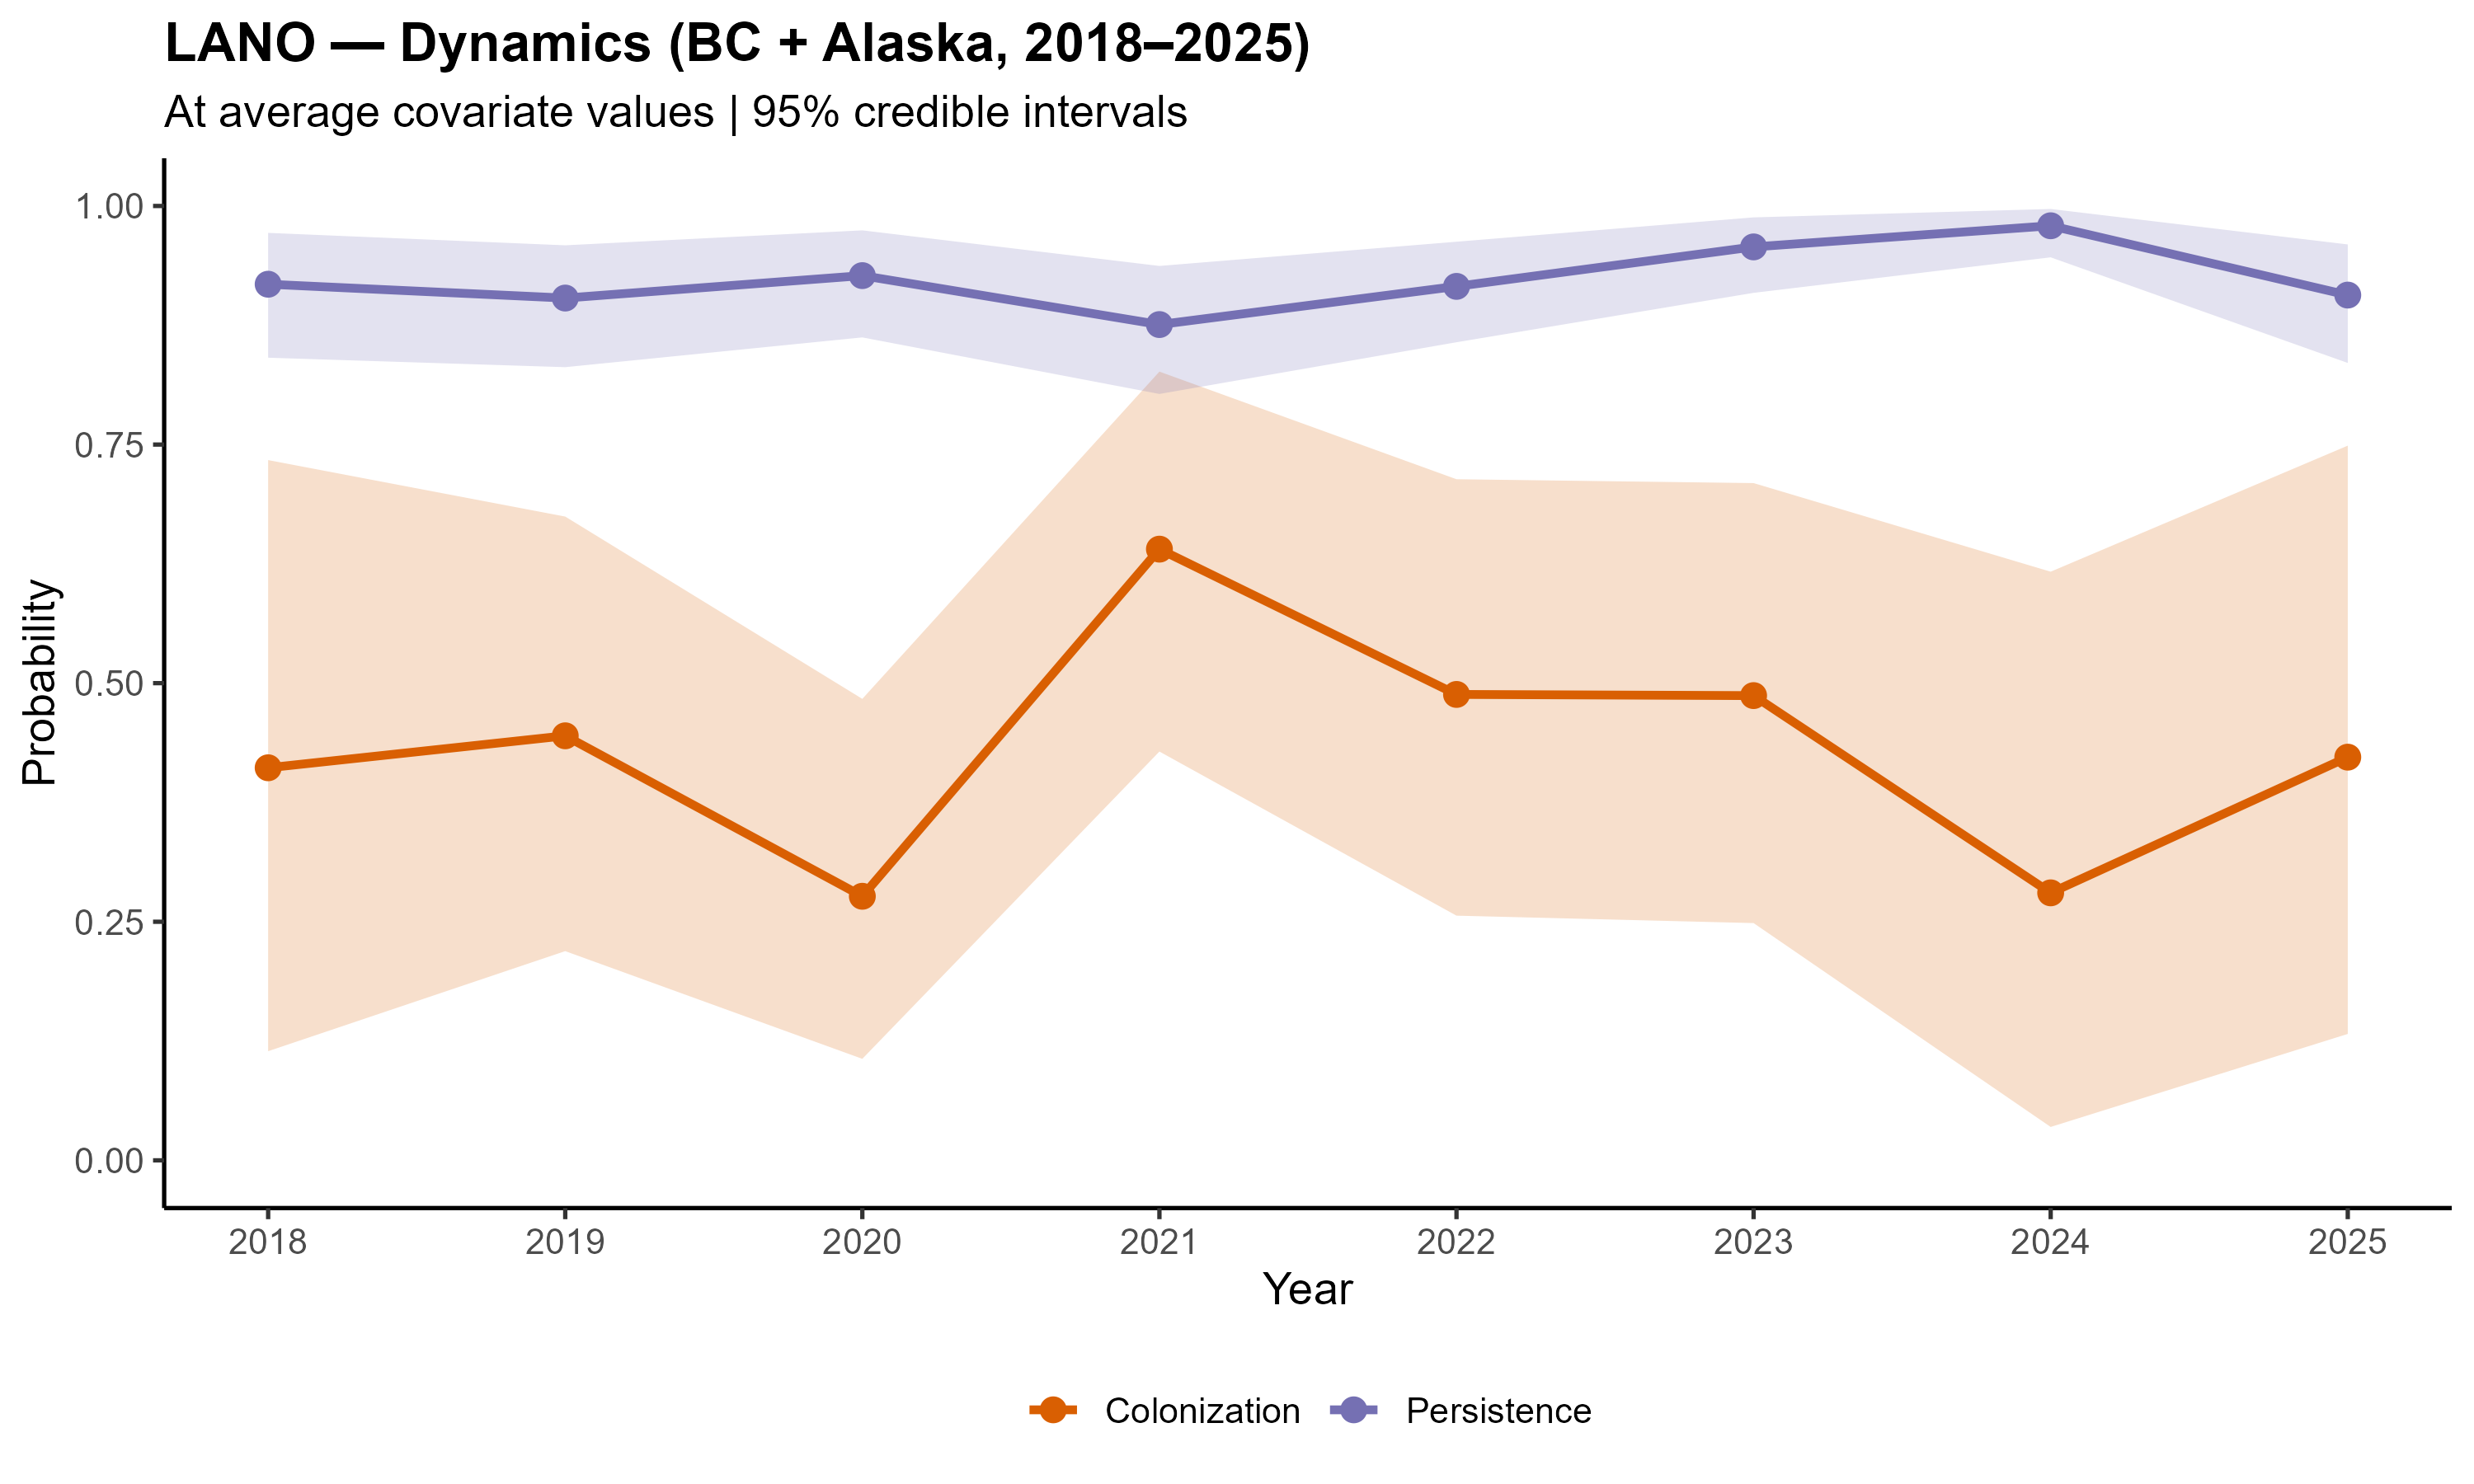
\includegraphics[keepaspectratio]{images/clipboard-950746085.png}}
\pandocbounded{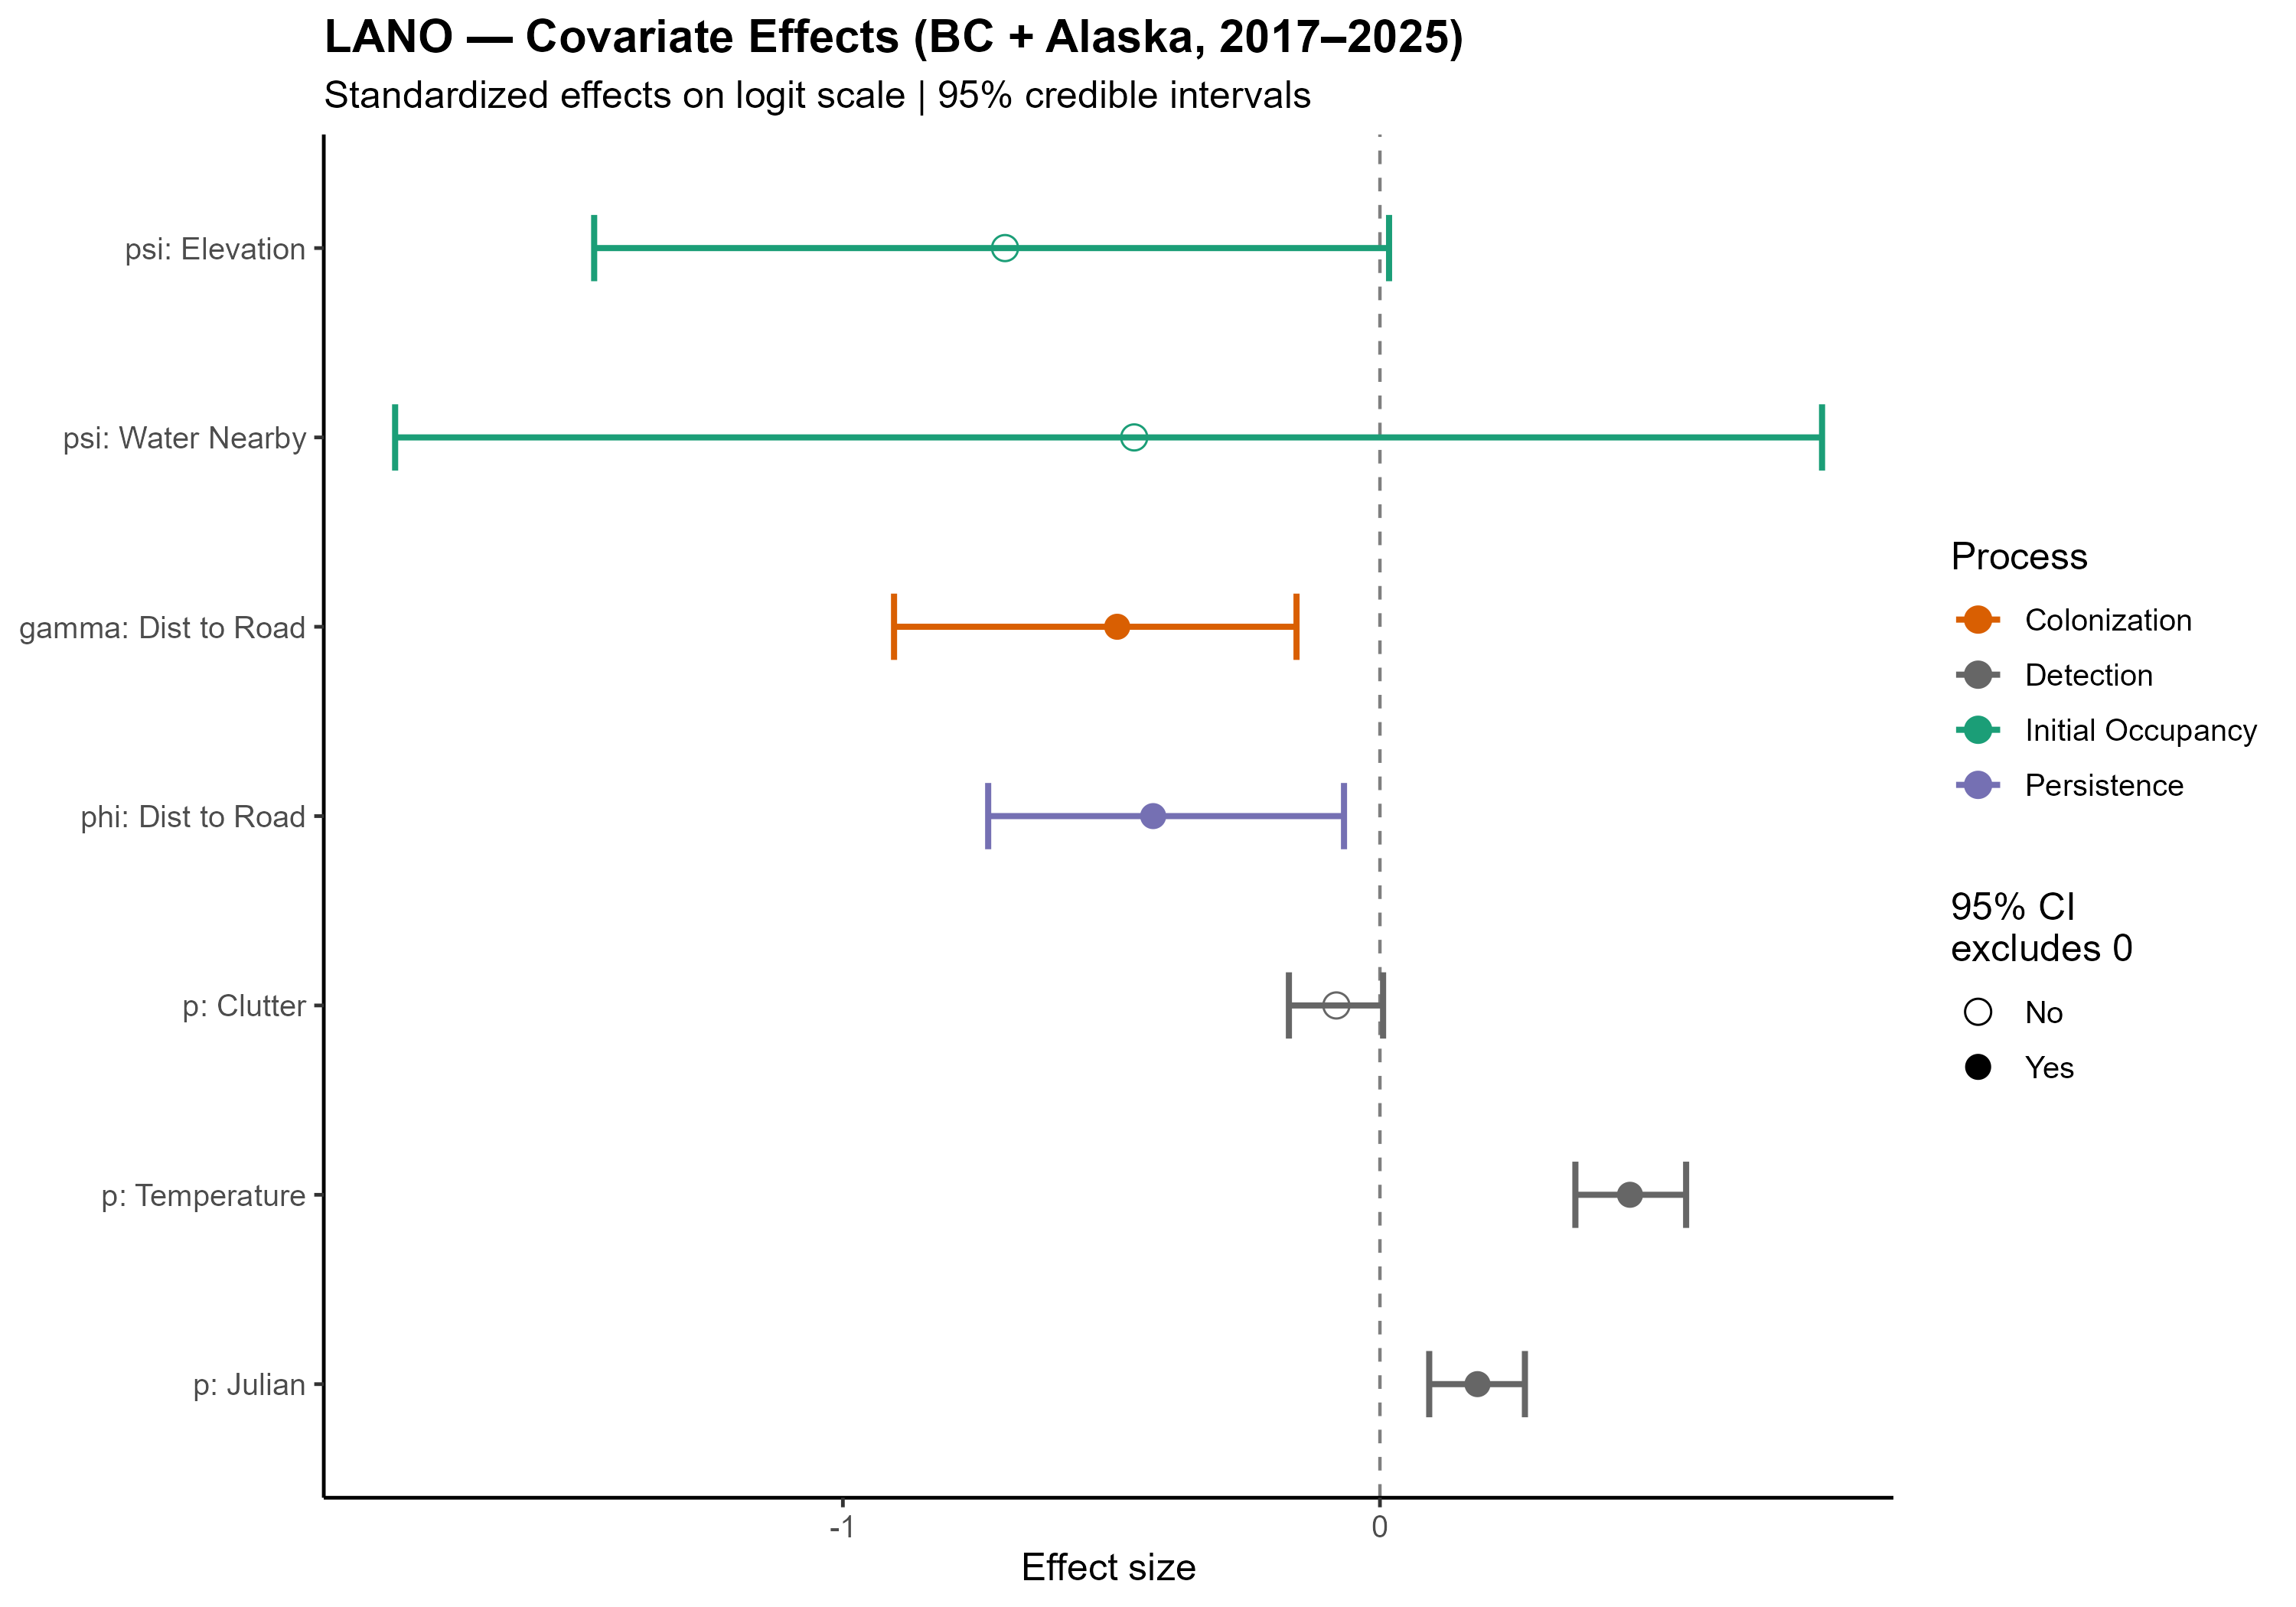
\includegraphics[keepaspectratio]{images/clipboard-4079169987.png}}

\subsection{\texorpdfstring{California Myotis (\emph{Myotis
californicus})}{California Myotis (Myotis californicus)}}\label{california-myotis-myotis-californicus}

\pandocbounded{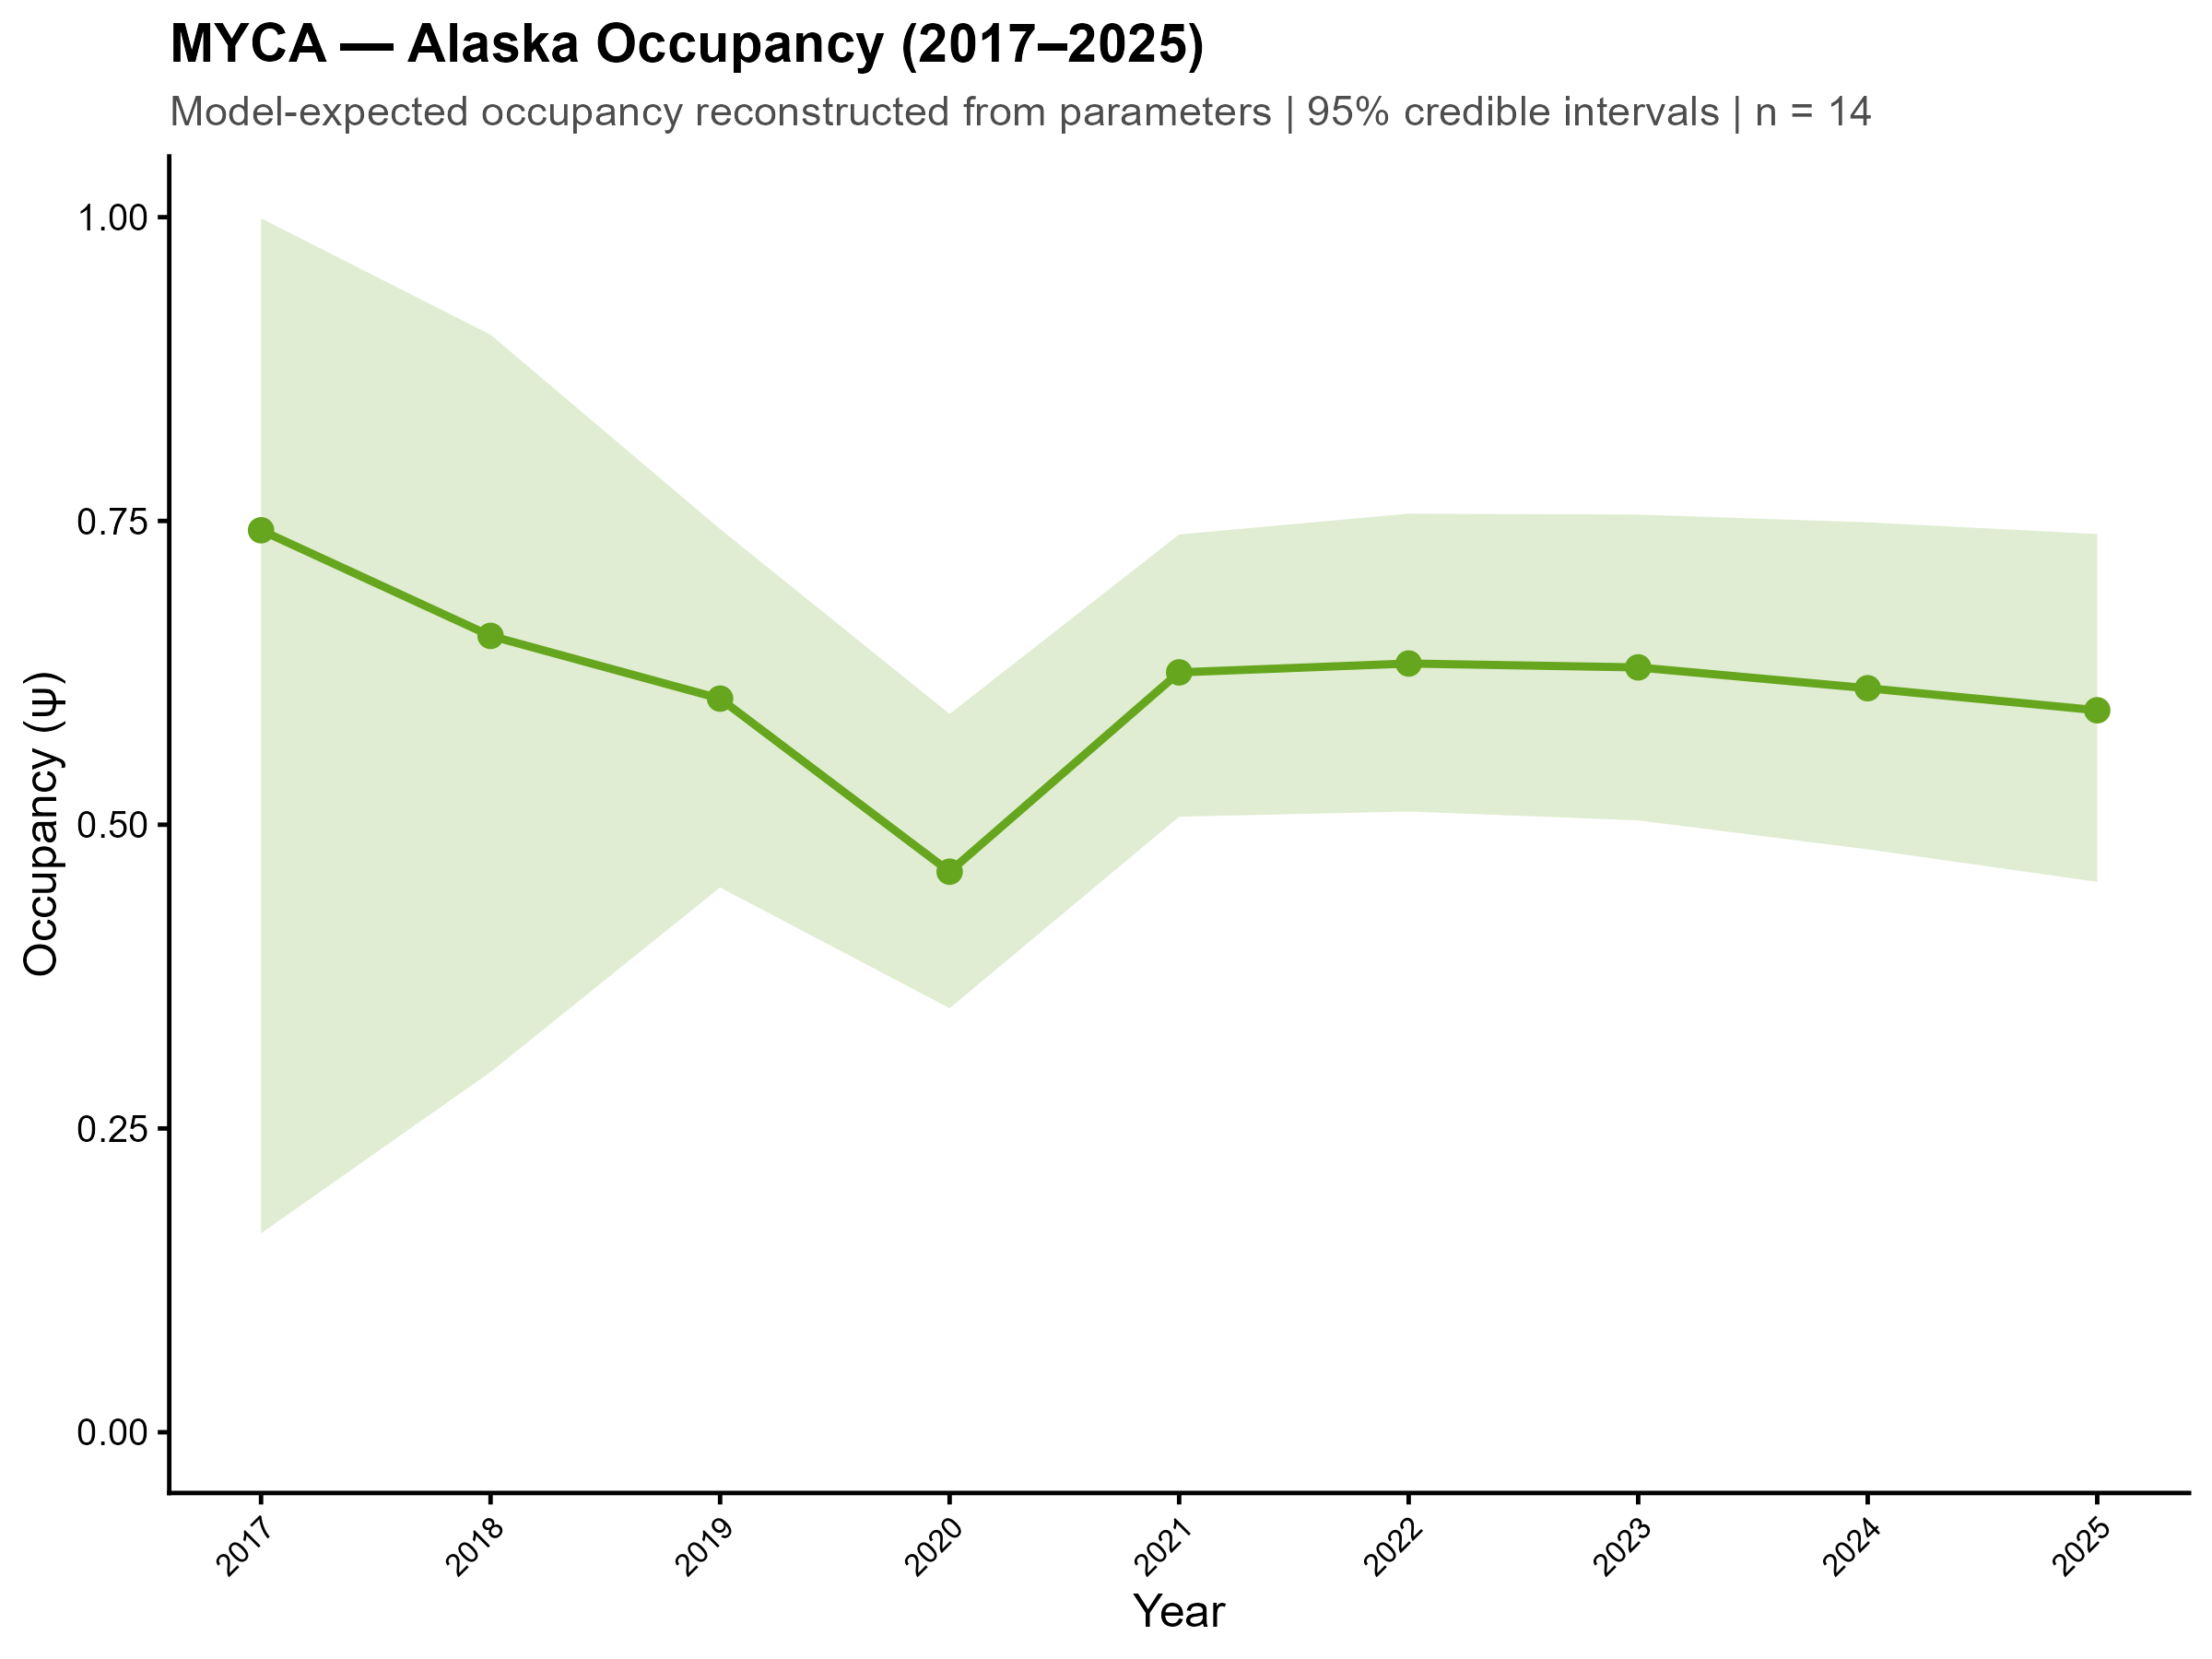
\includegraphics[keepaspectratio]{images/clipboard-2427323019.png}}
\pandocbounded{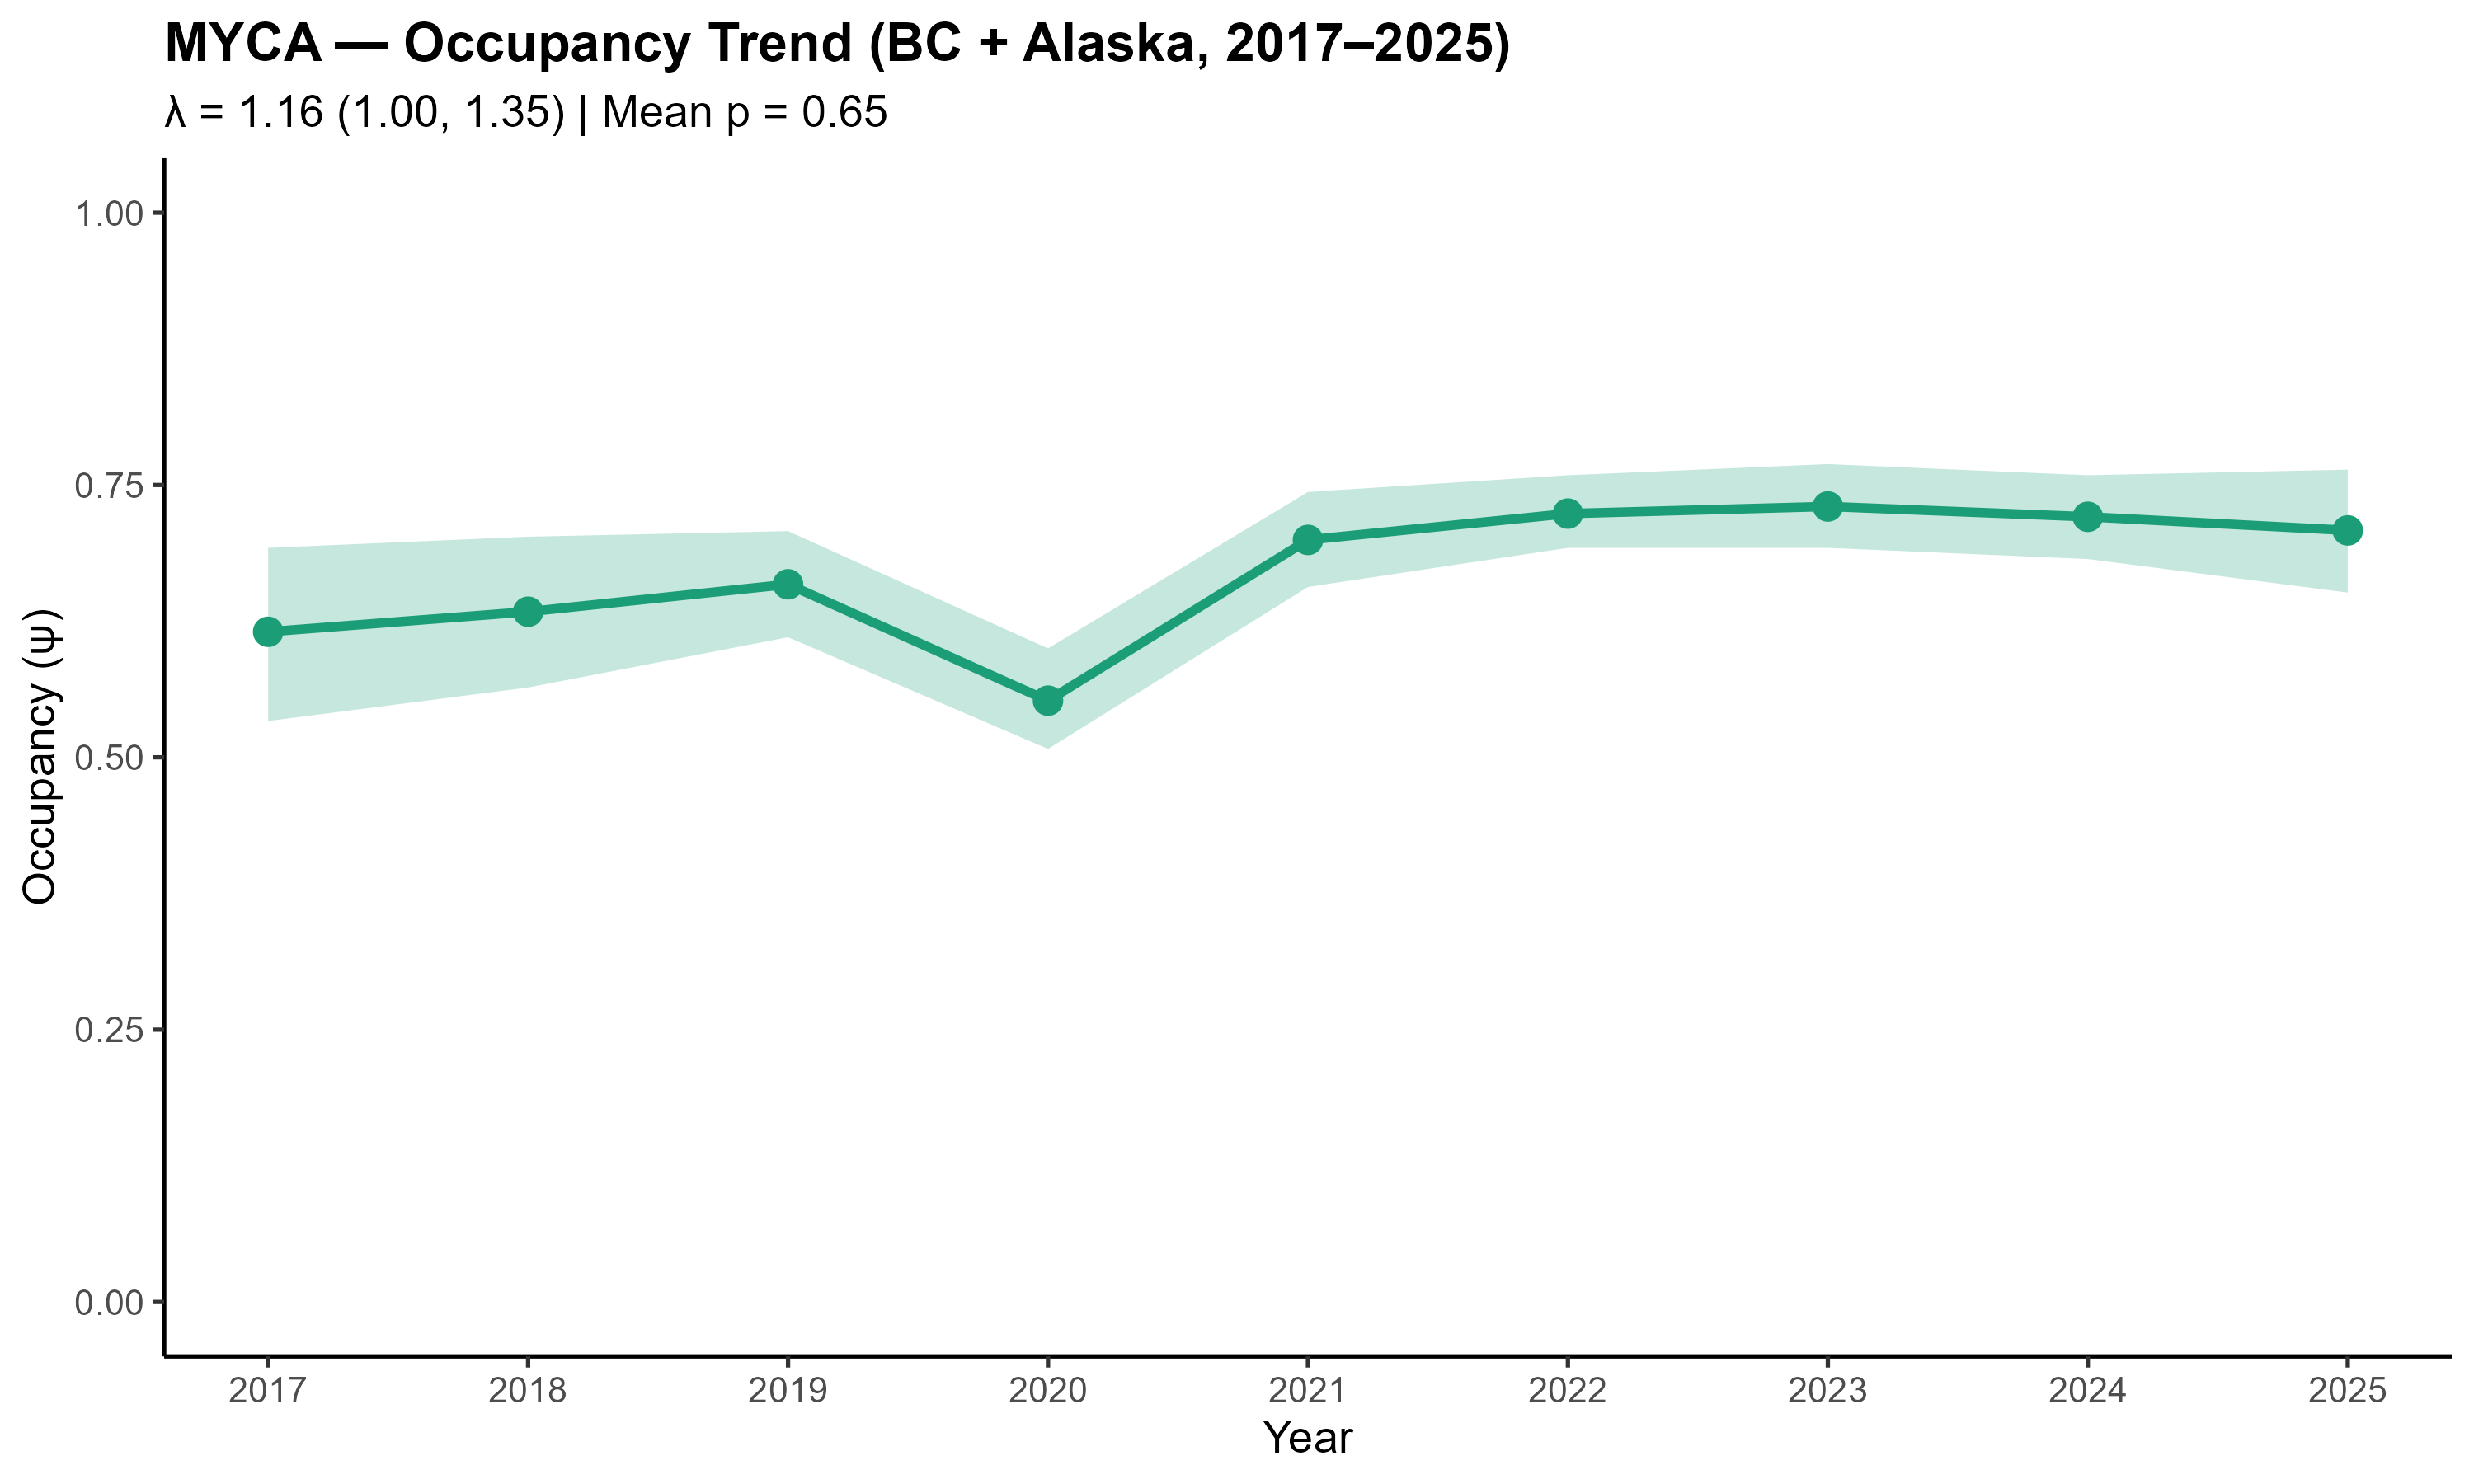
\includegraphics[keepaspectratio]{images/clipboard-359804971.png}}
\pandocbounded{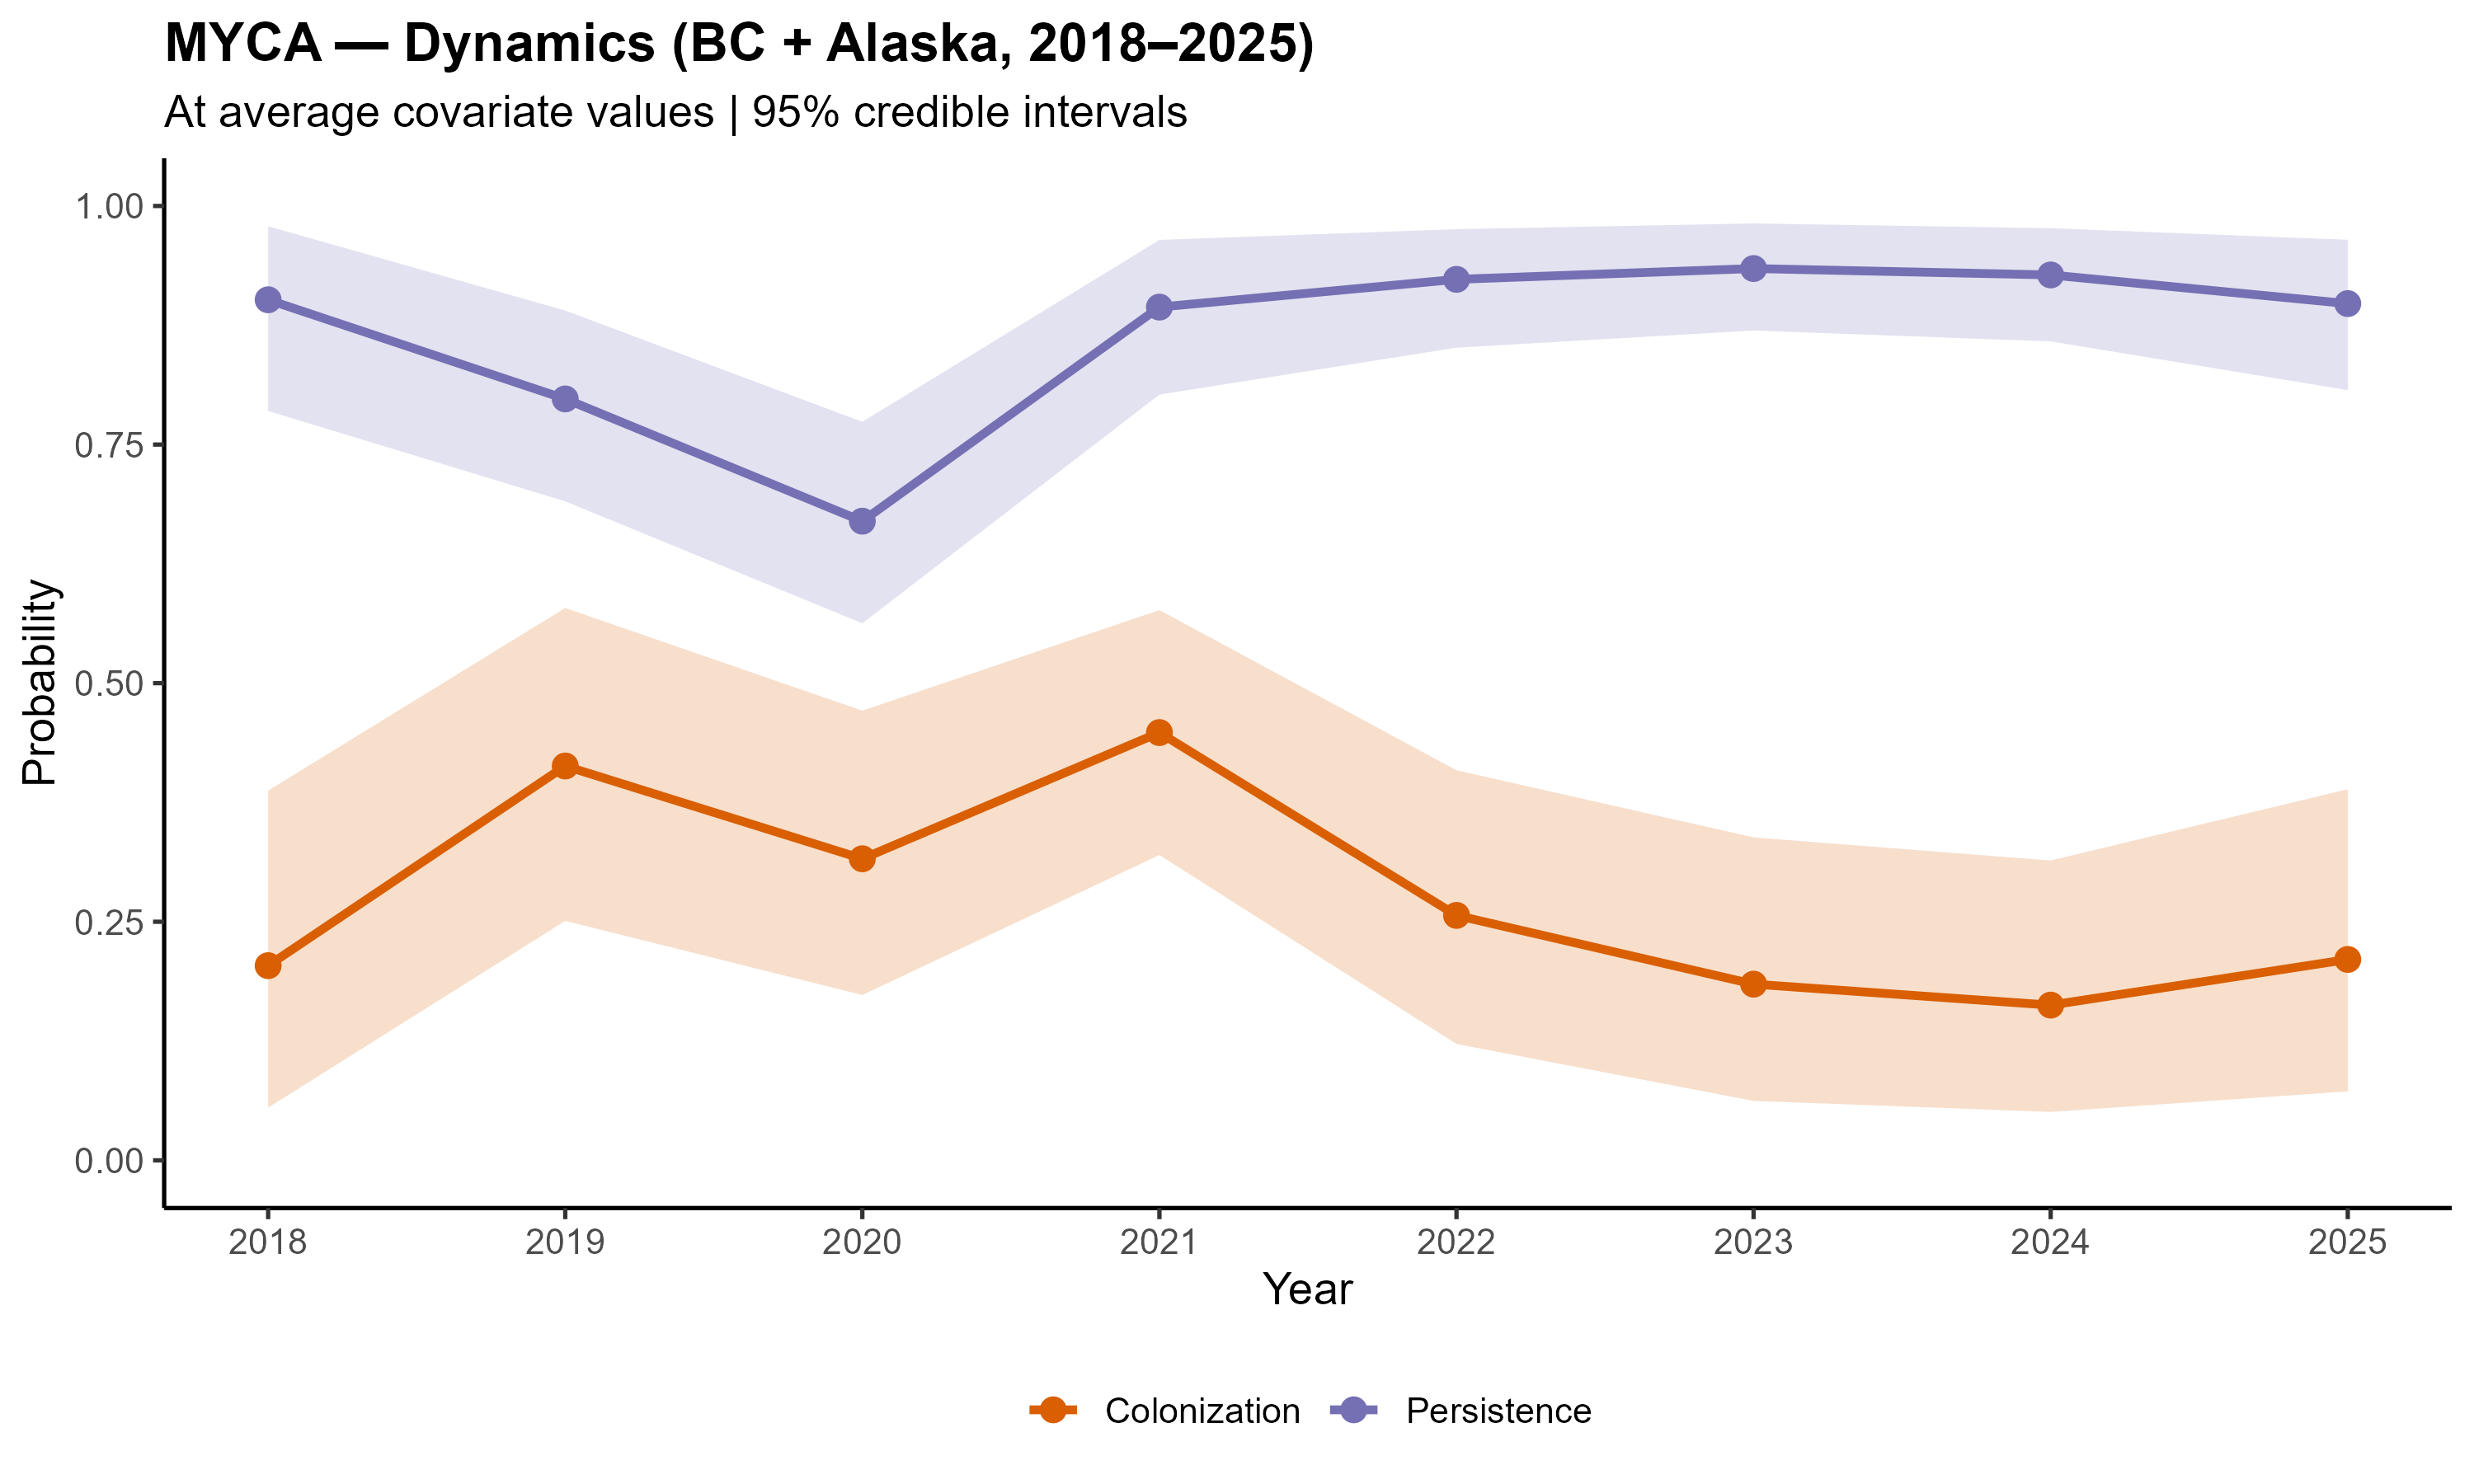
\includegraphics[keepaspectratio]{images/clipboard-3695743881.png}}
\pandocbounded{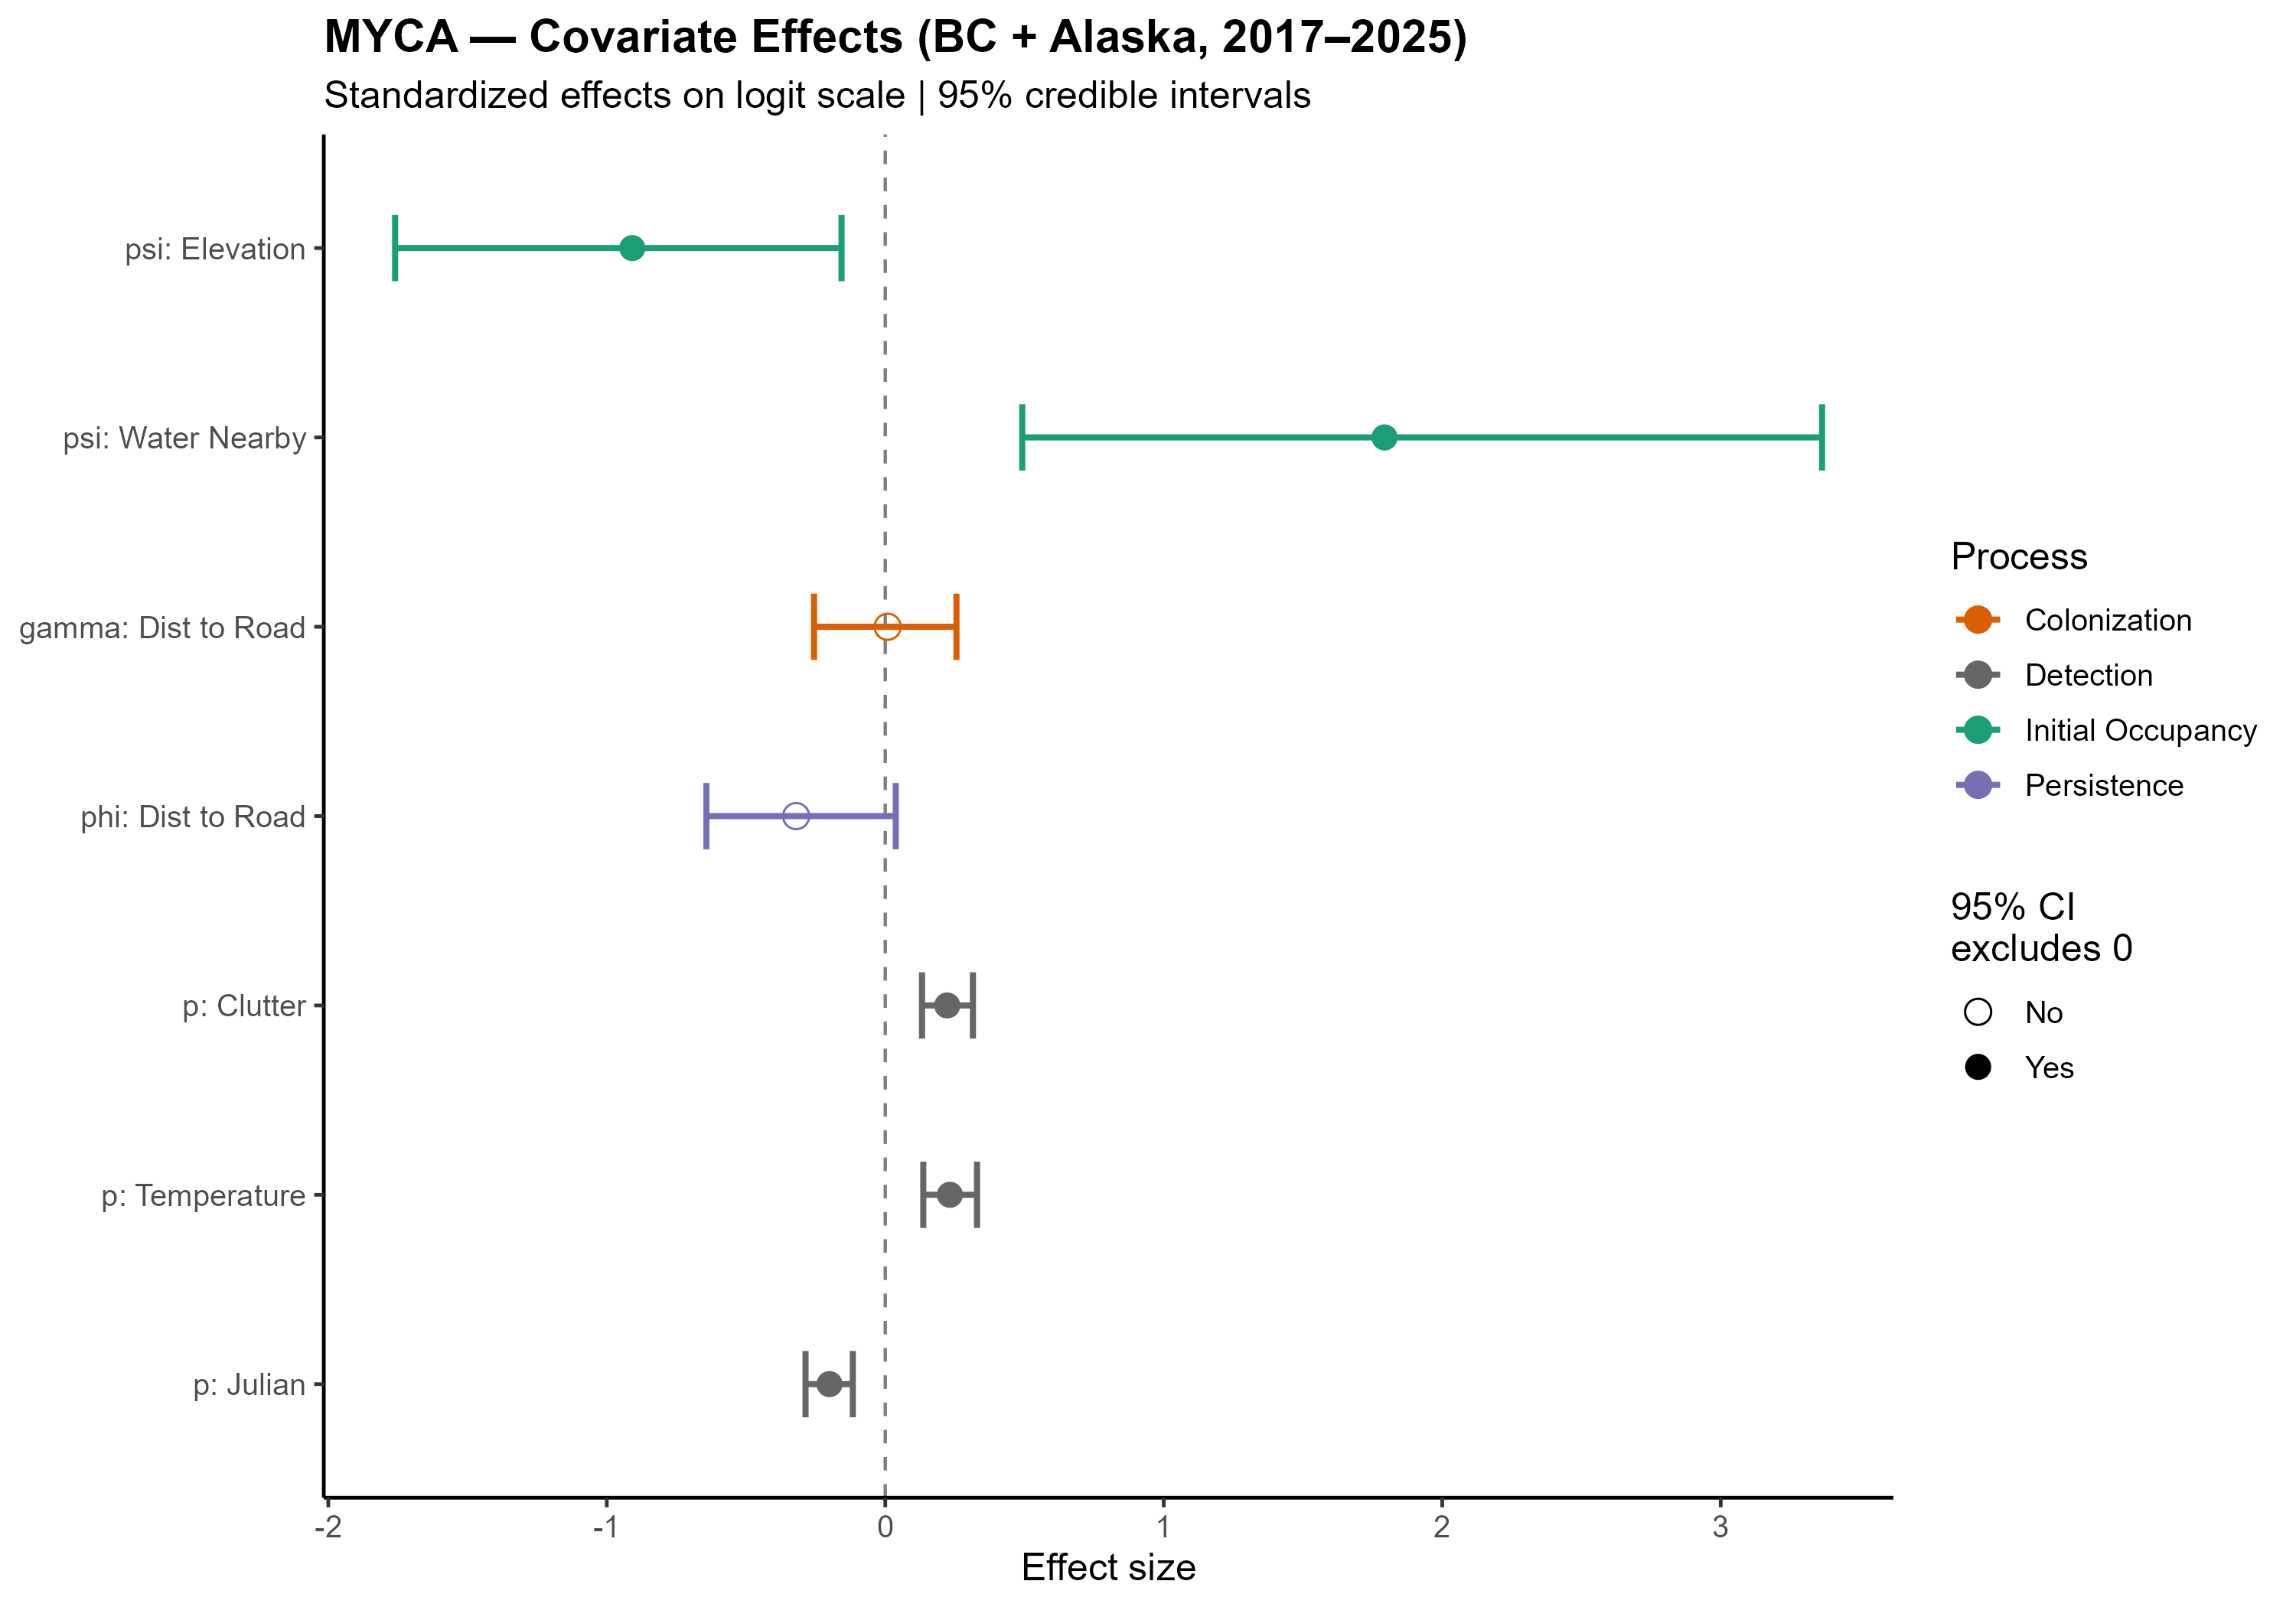
\includegraphics[keepaspectratio]{images/clipboard-1493695761.png}}

\subsection{\texorpdfstring{Long-eared Myotis (\emph{Myotis
evotis})}{Long-eared Myotis (Myotis evotis)}}\label{long-eared-myotis-myotis-evotis}

\pandocbounded{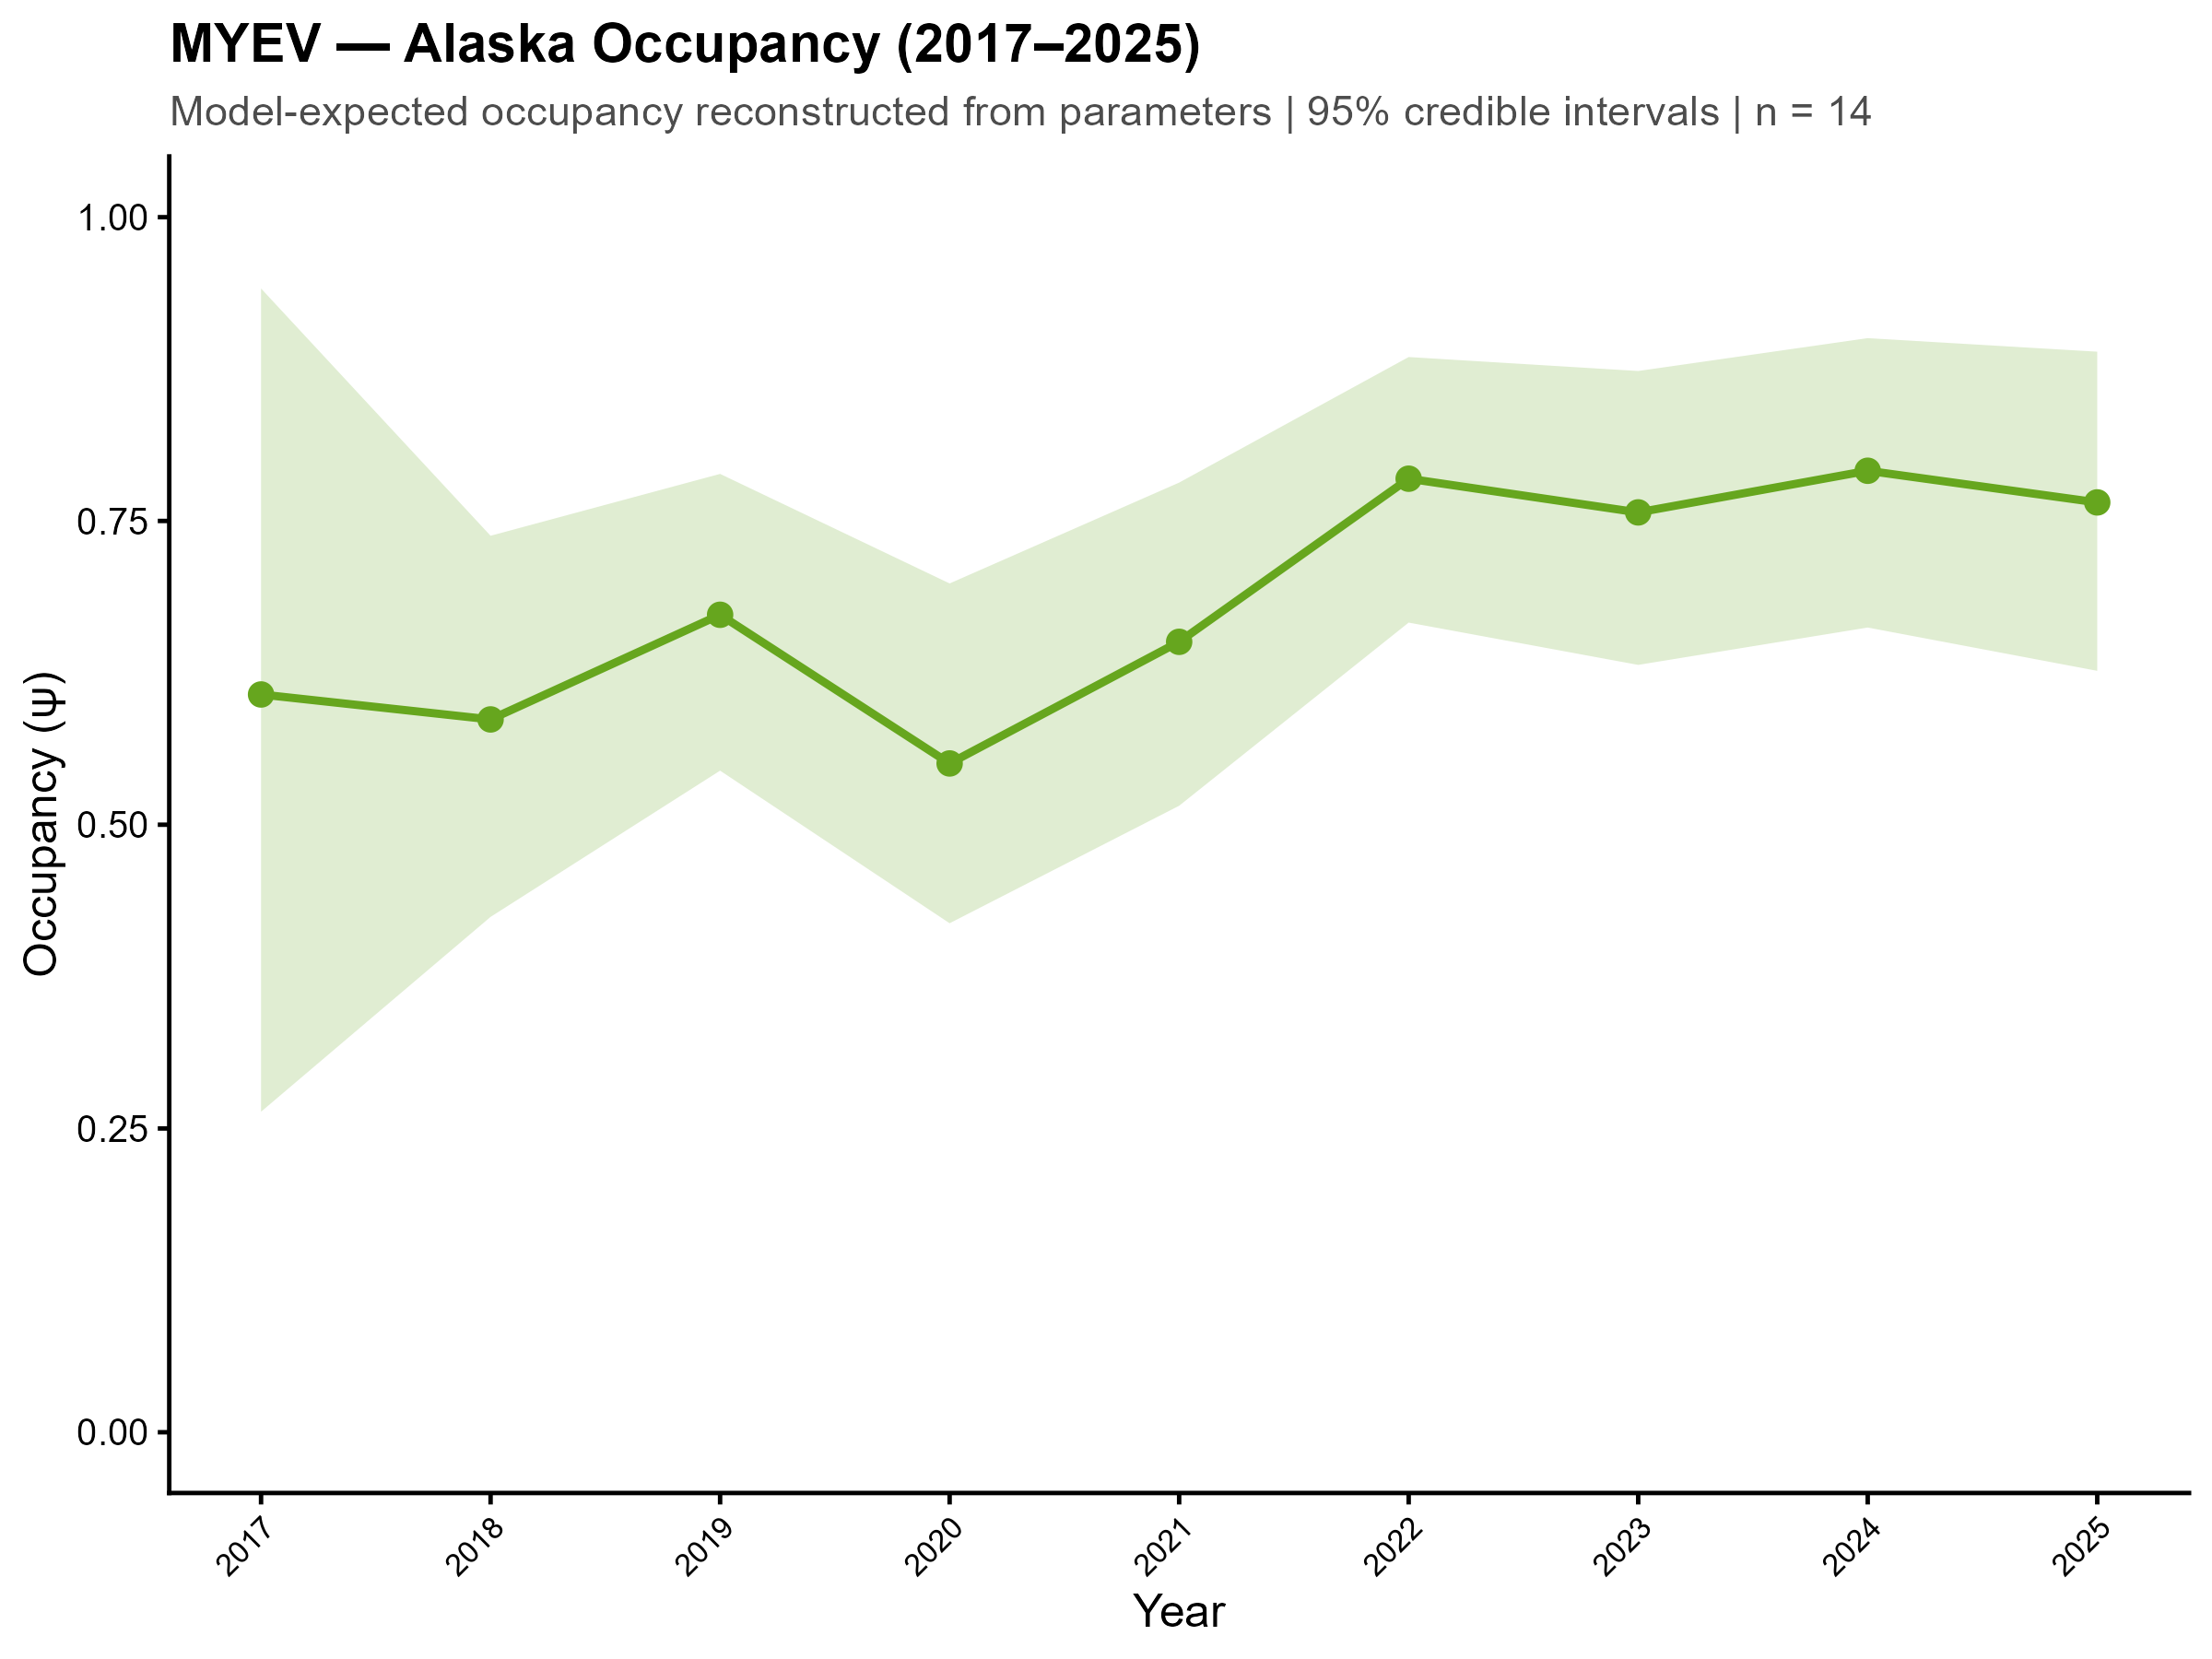
\includegraphics[keepaspectratio]{images/clipboard-3941761601.png}}
\pandocbounded{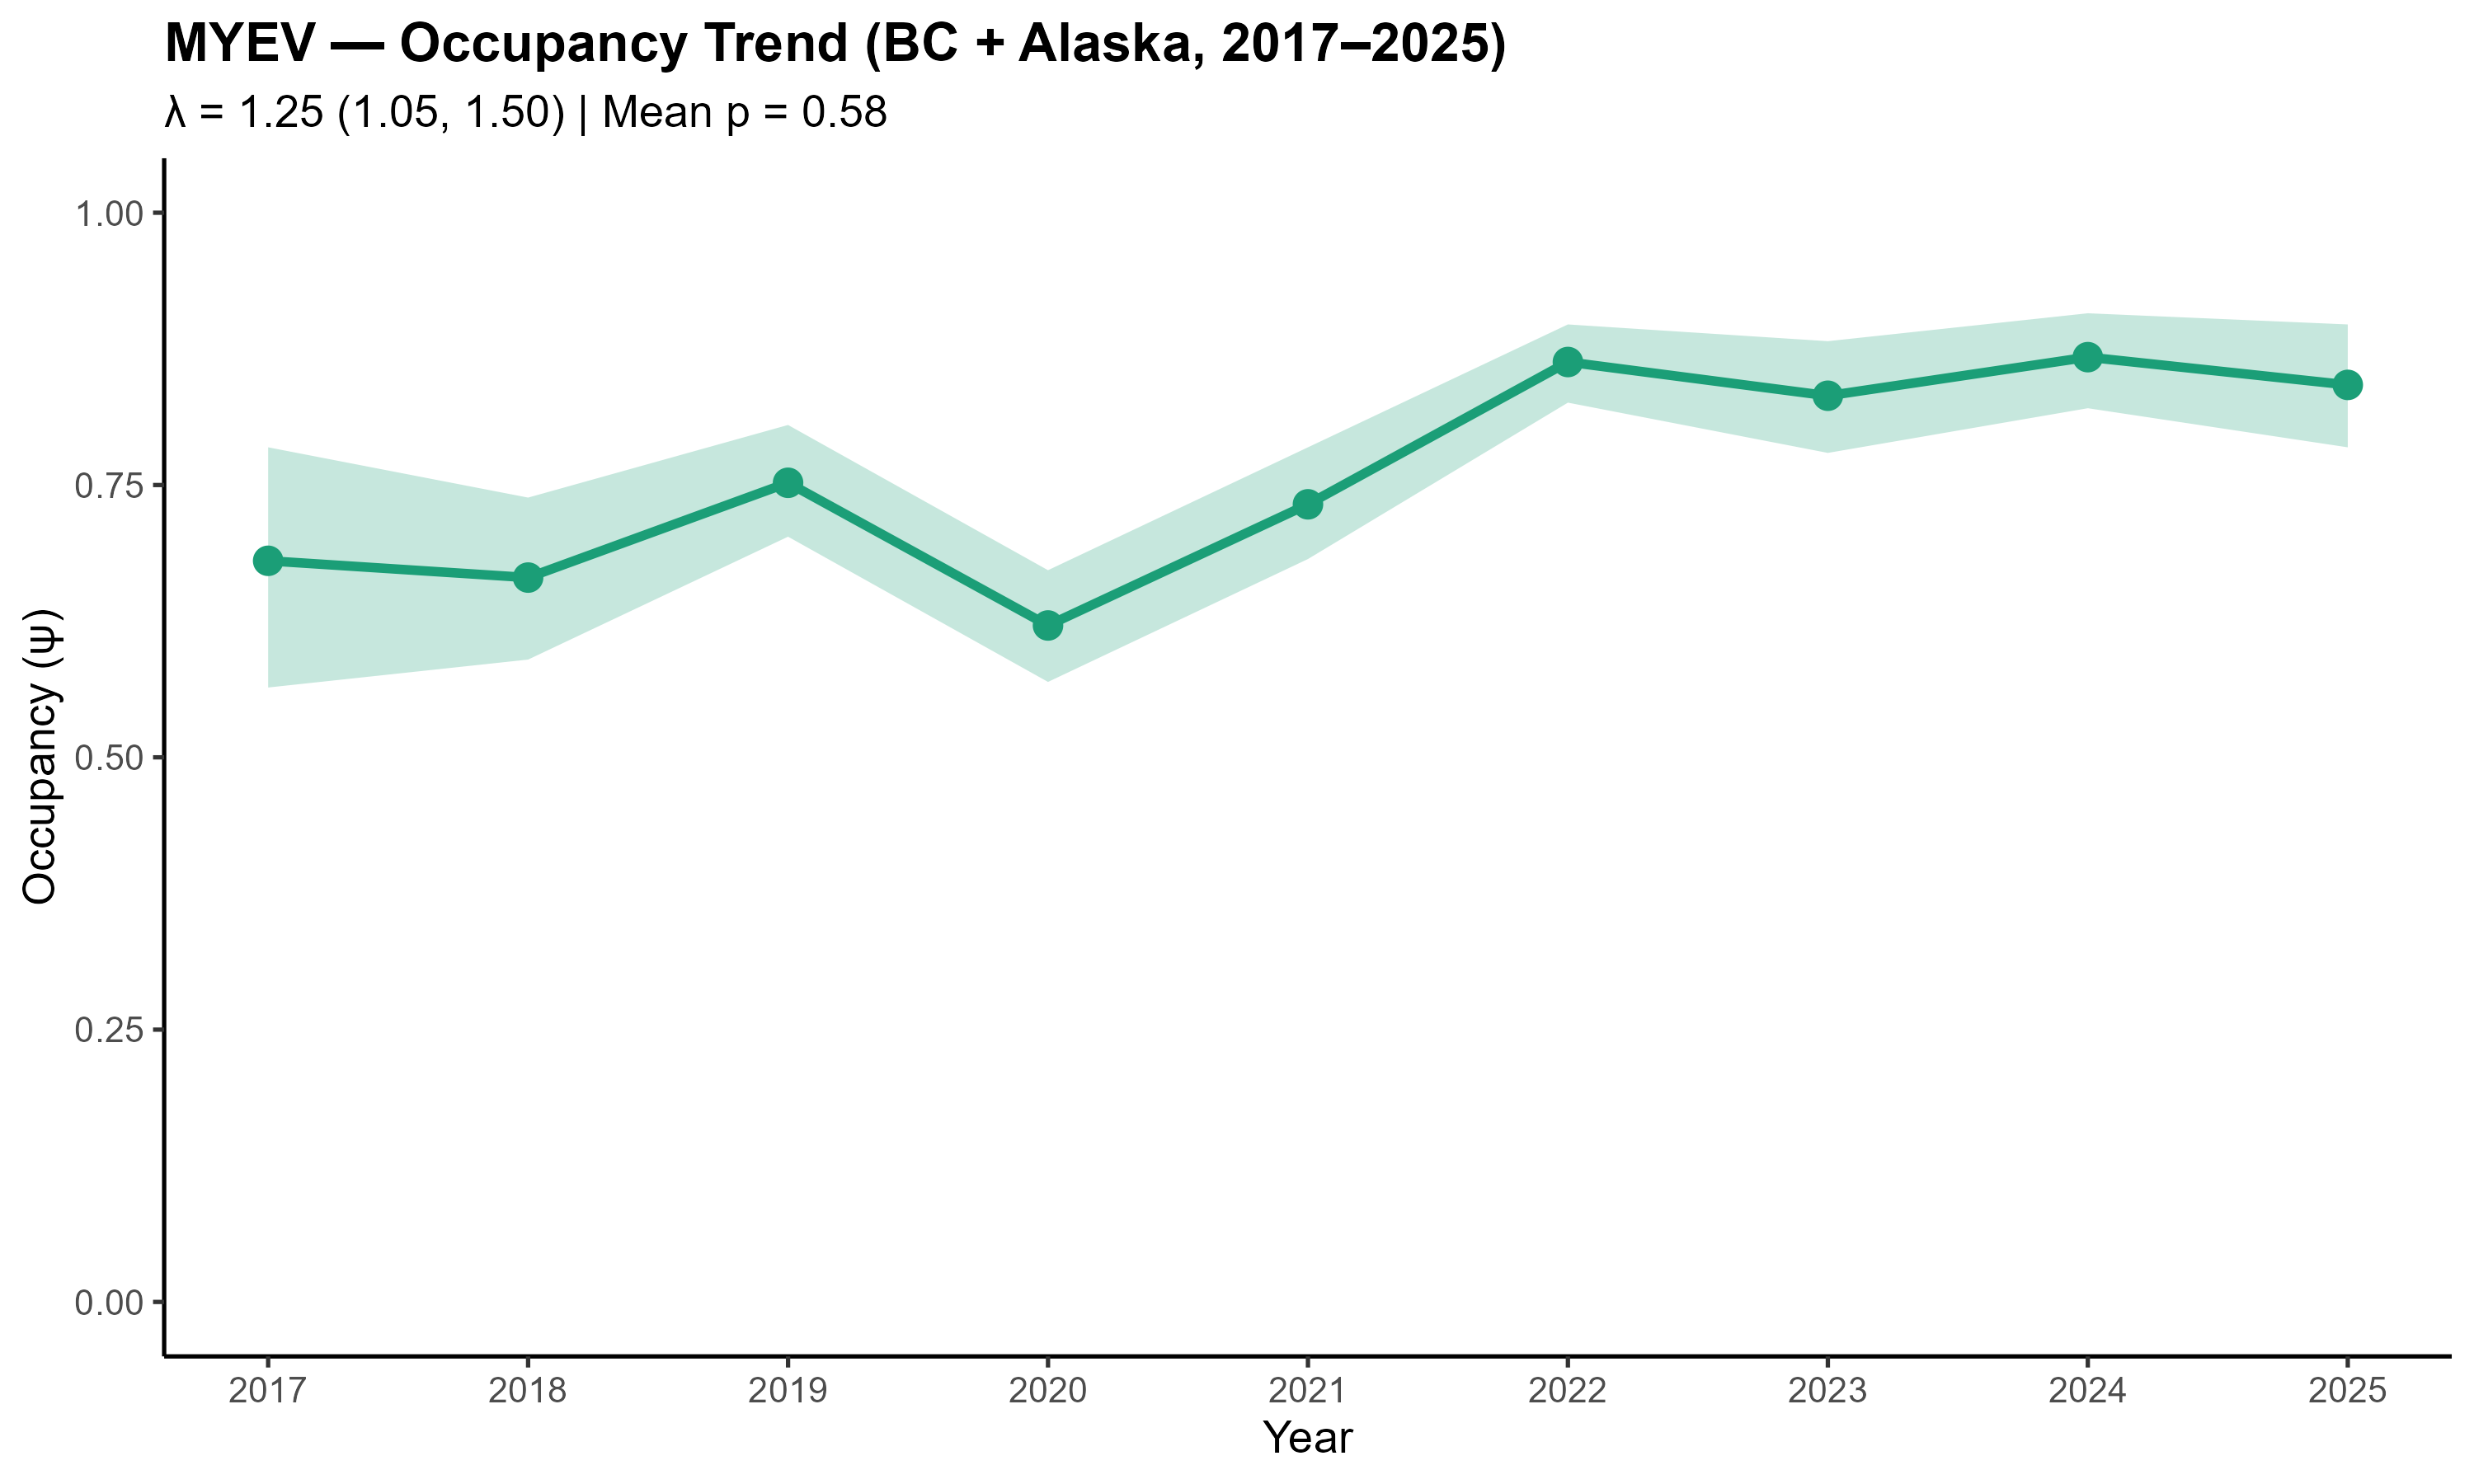
\includegraphics[keepaspectratio]{images/clipboard-2730898759.png}}
\pandocbounded{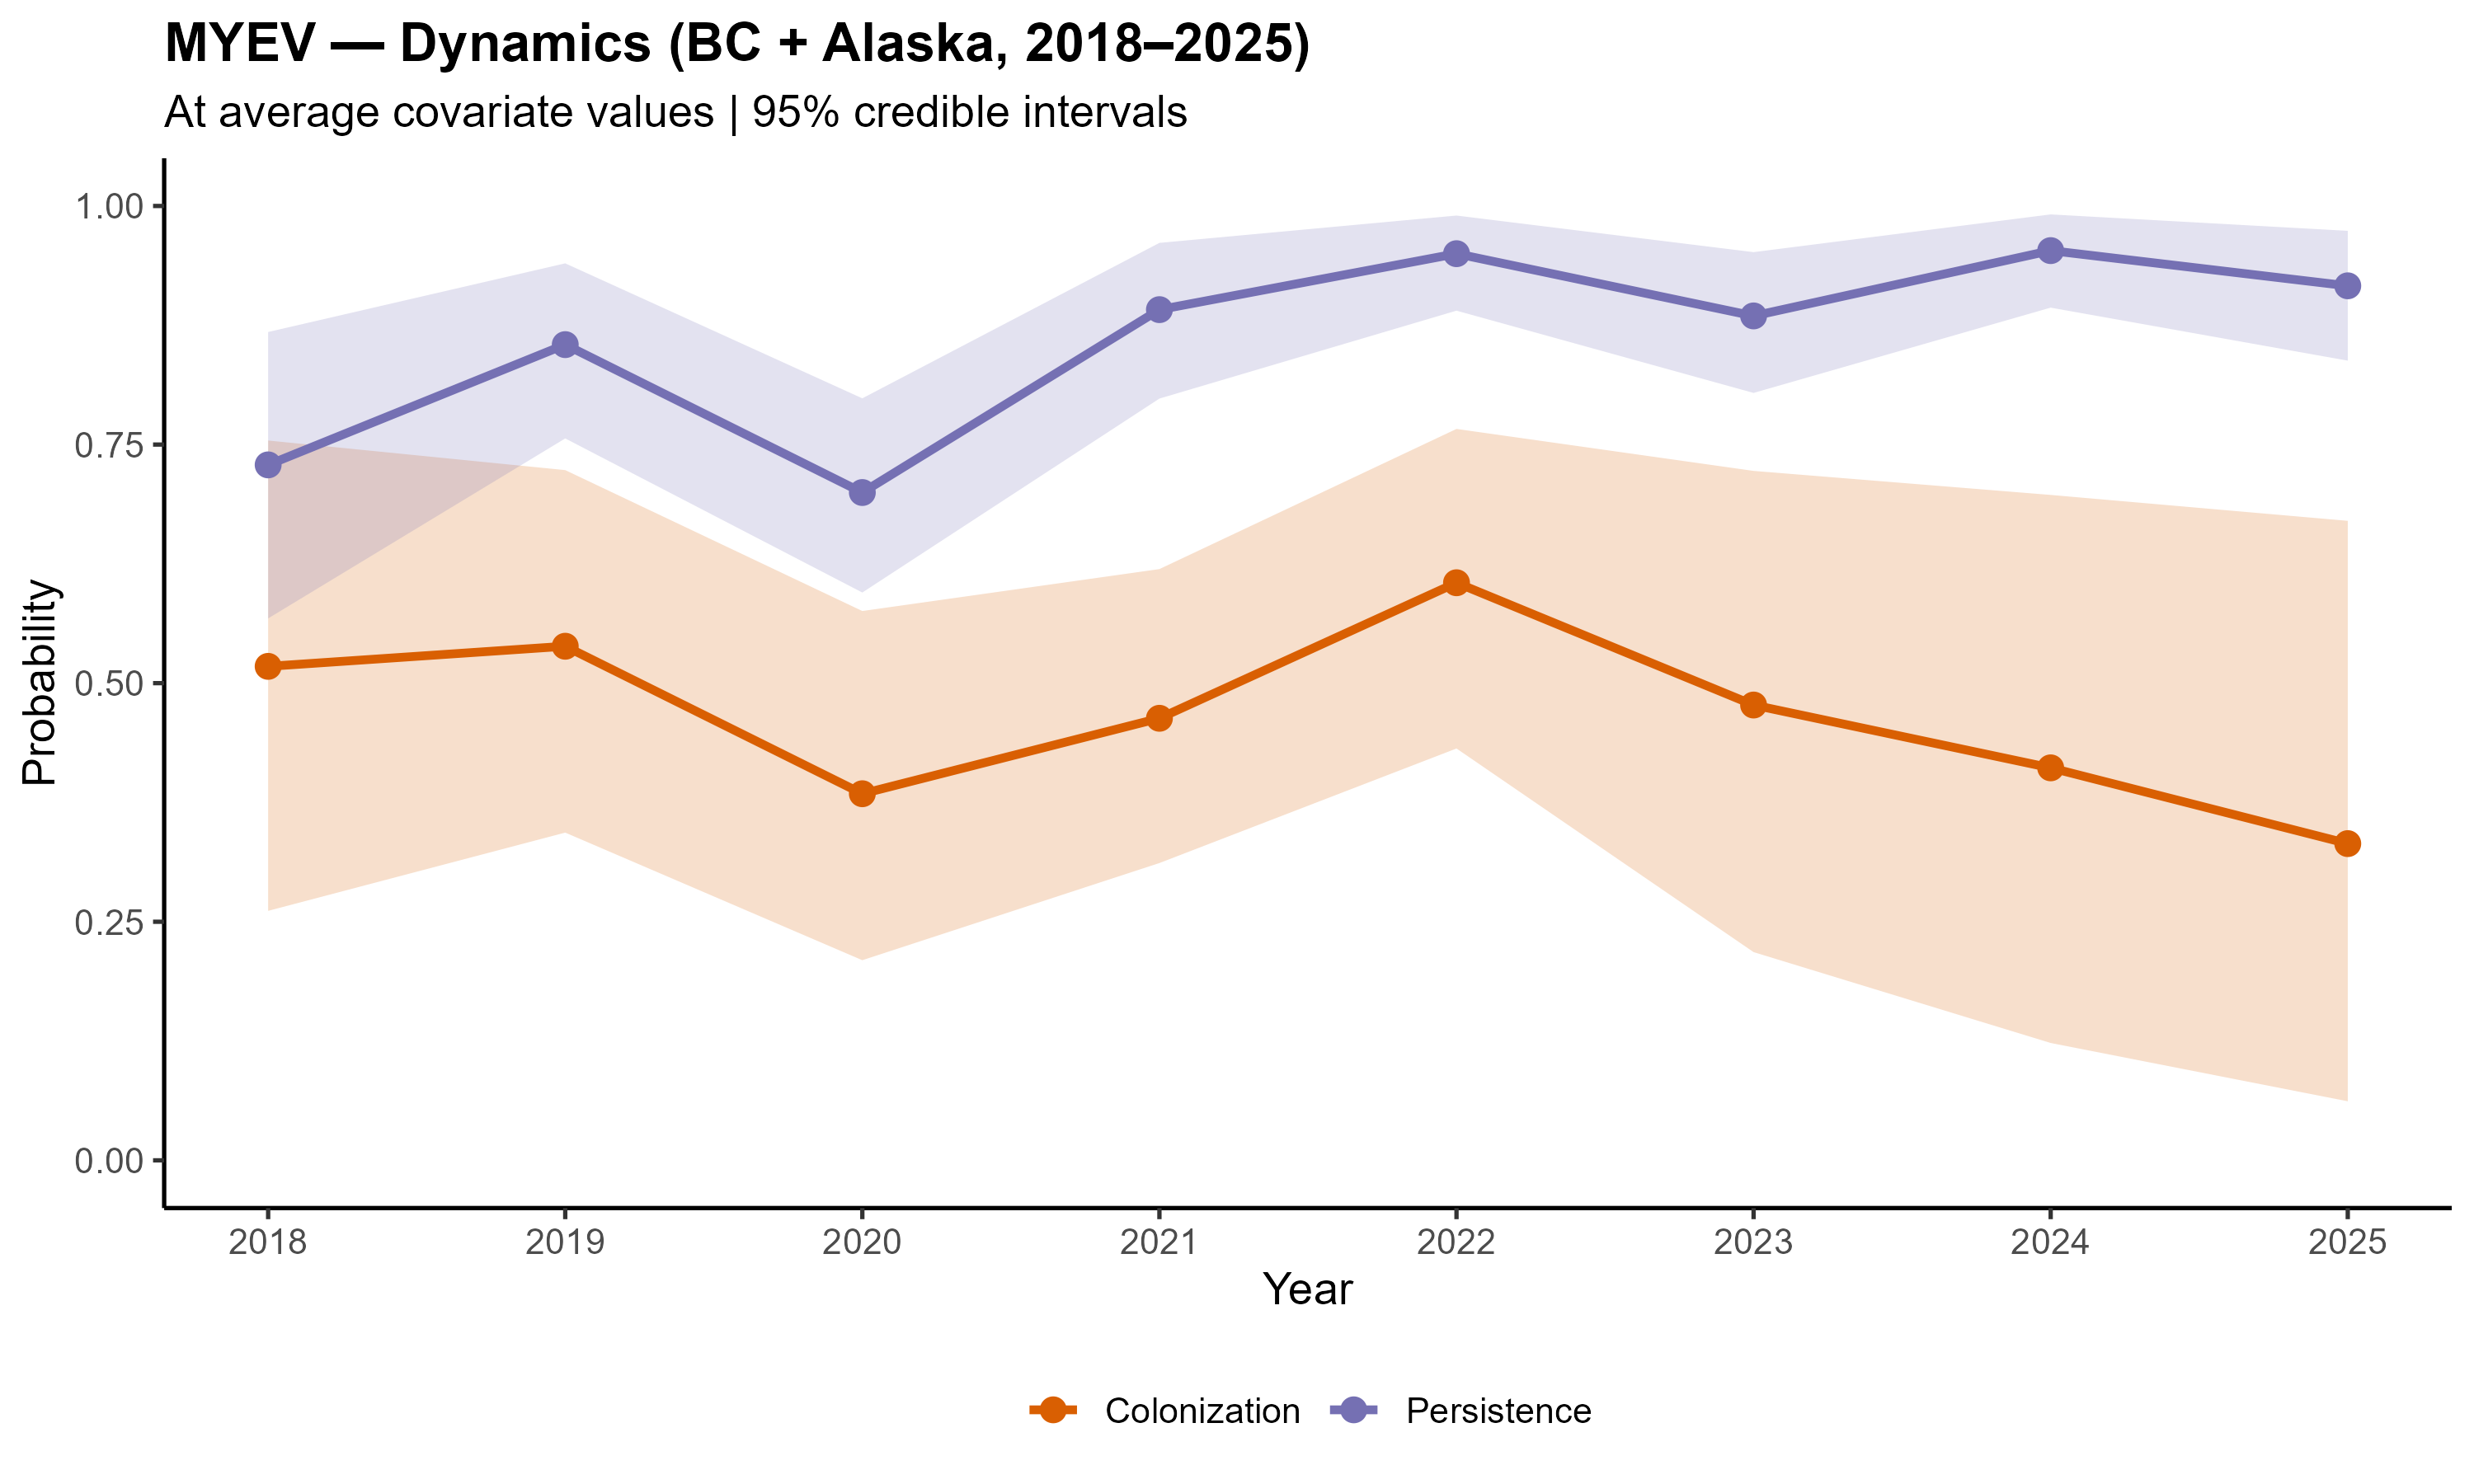
\includegraphics[keepaspectratio]{images/clipboard-3987187980.png}}
\pandocbounded{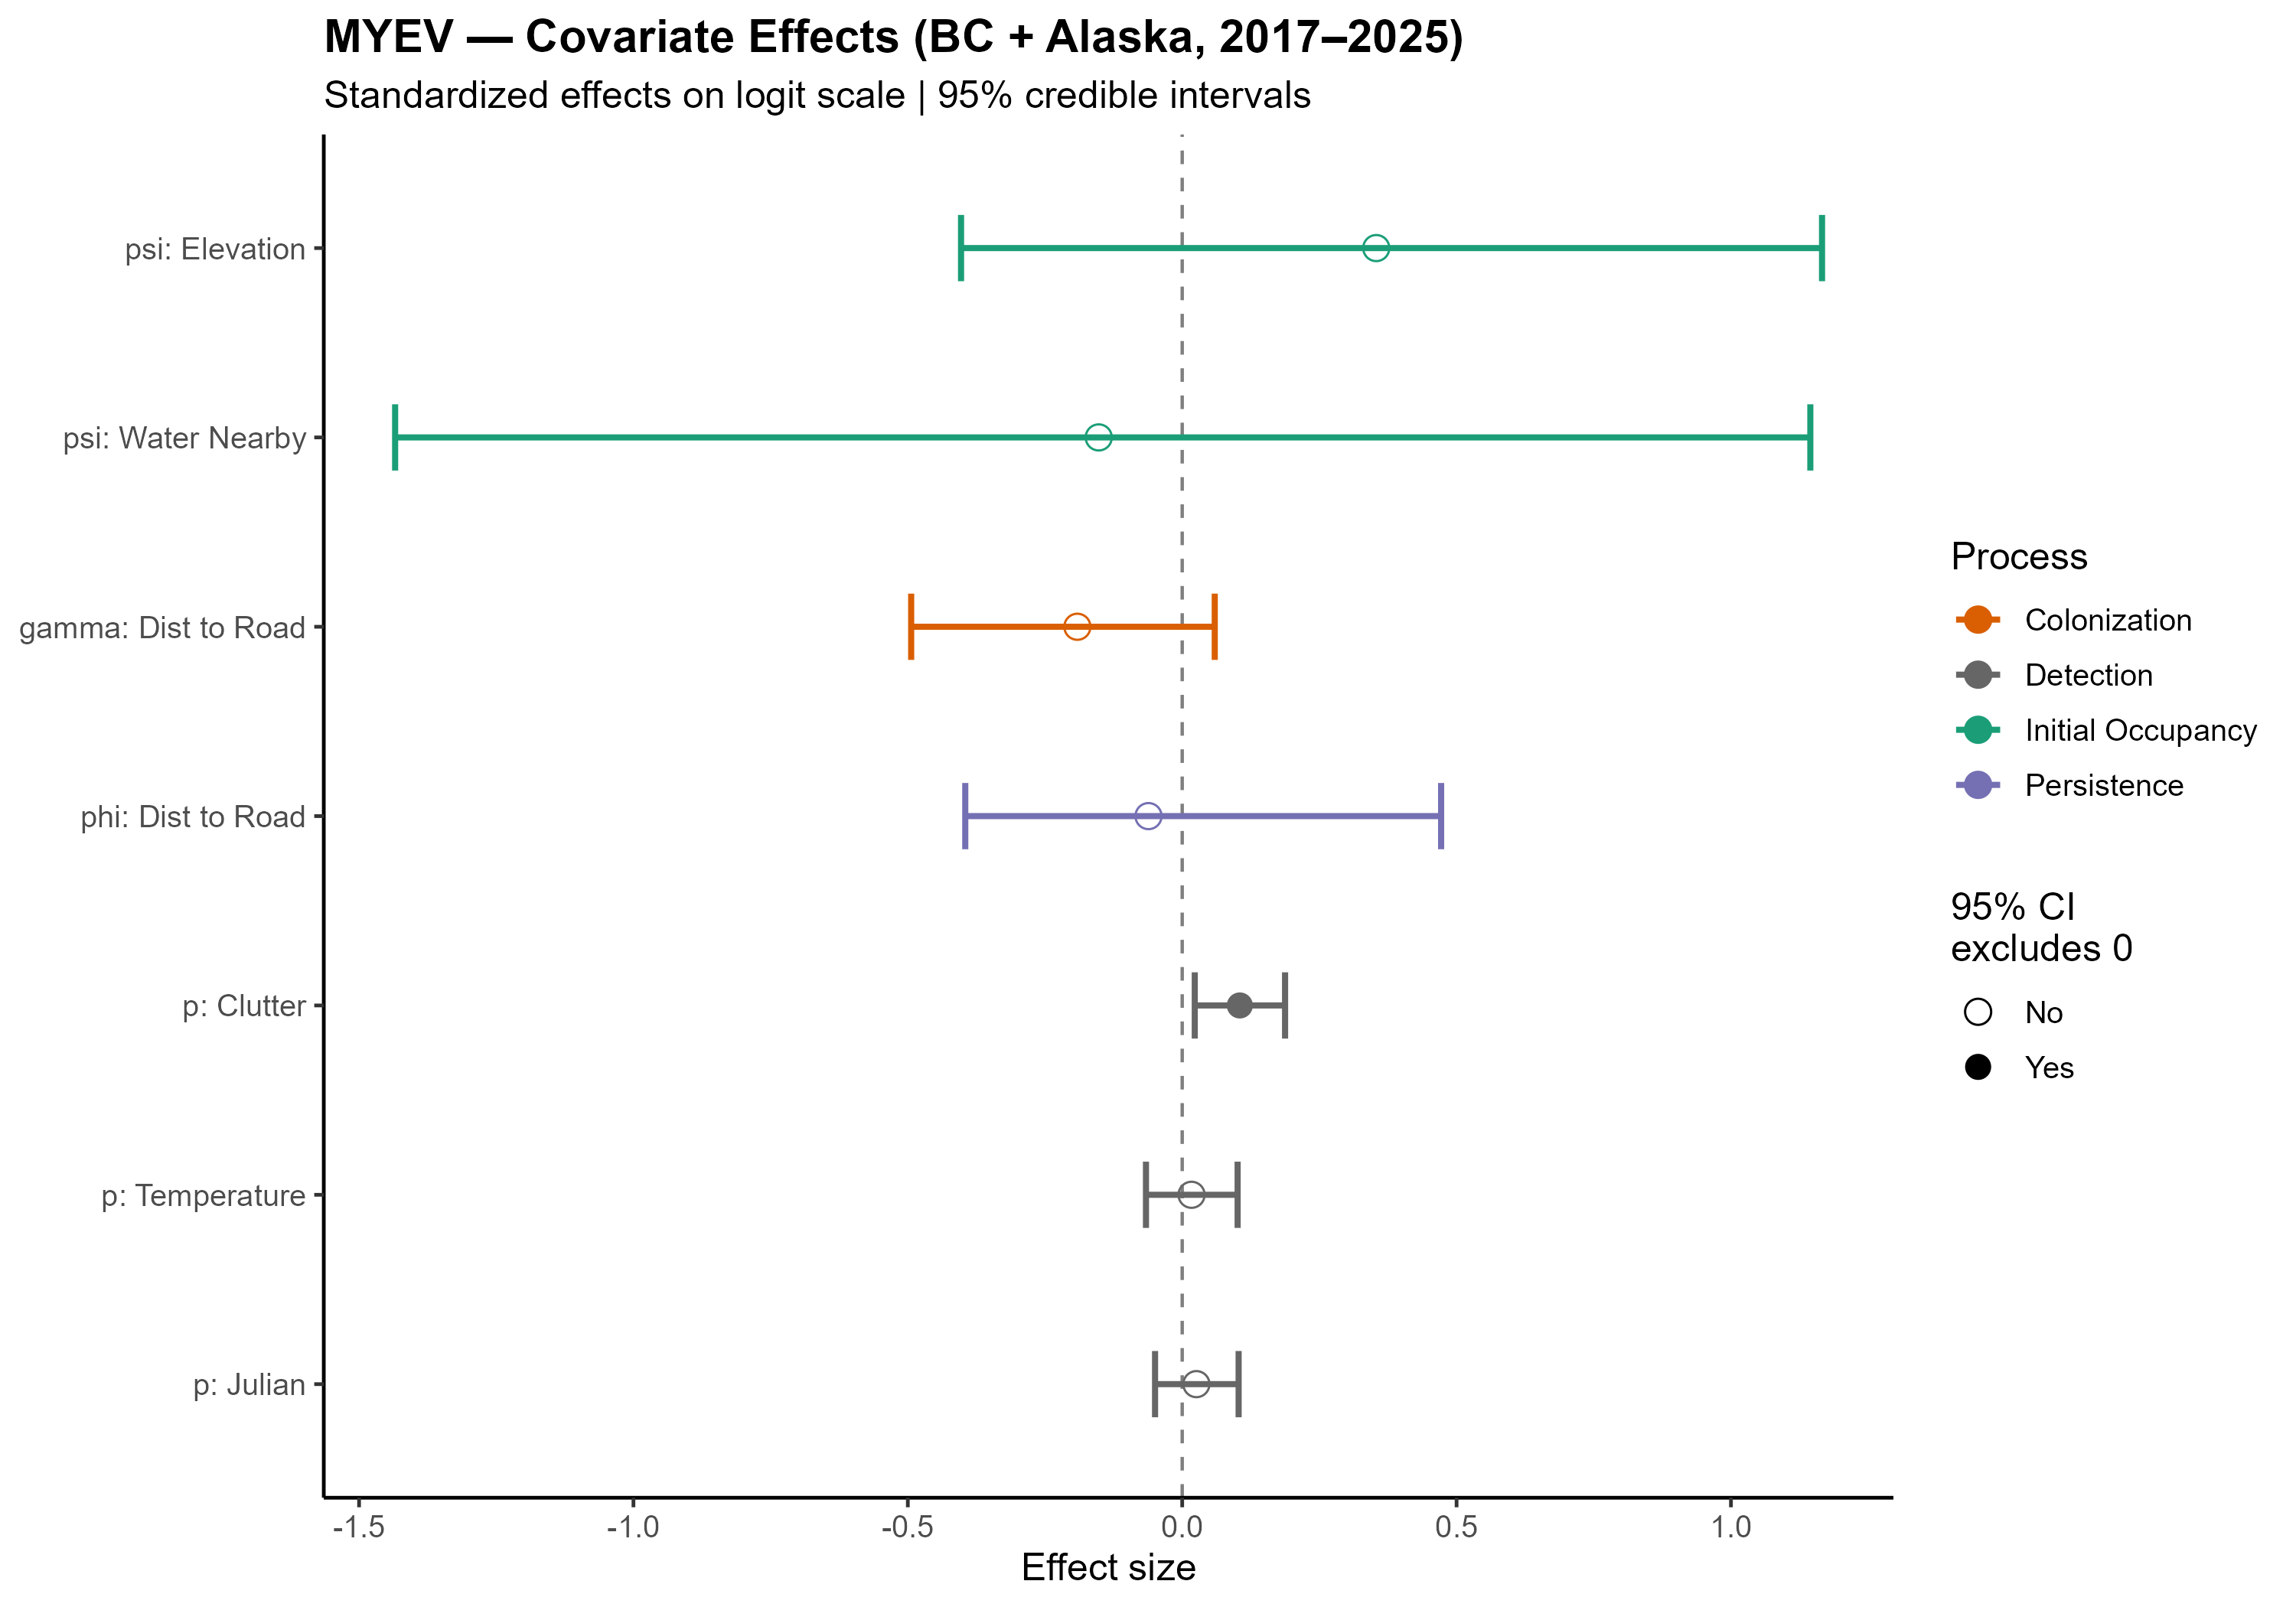
\includegraphics[keepaspectratio]{images/clipboard-3555136292.png}}

\subsection{\texorpdfstring{Little Brown Myotis (\emph{Myotis
lucifugus})}{Little Brown Myotis (Myotis lucifugus)}}\label{little-brown-myotis-myotis-lucifugus}

\pandocbounded{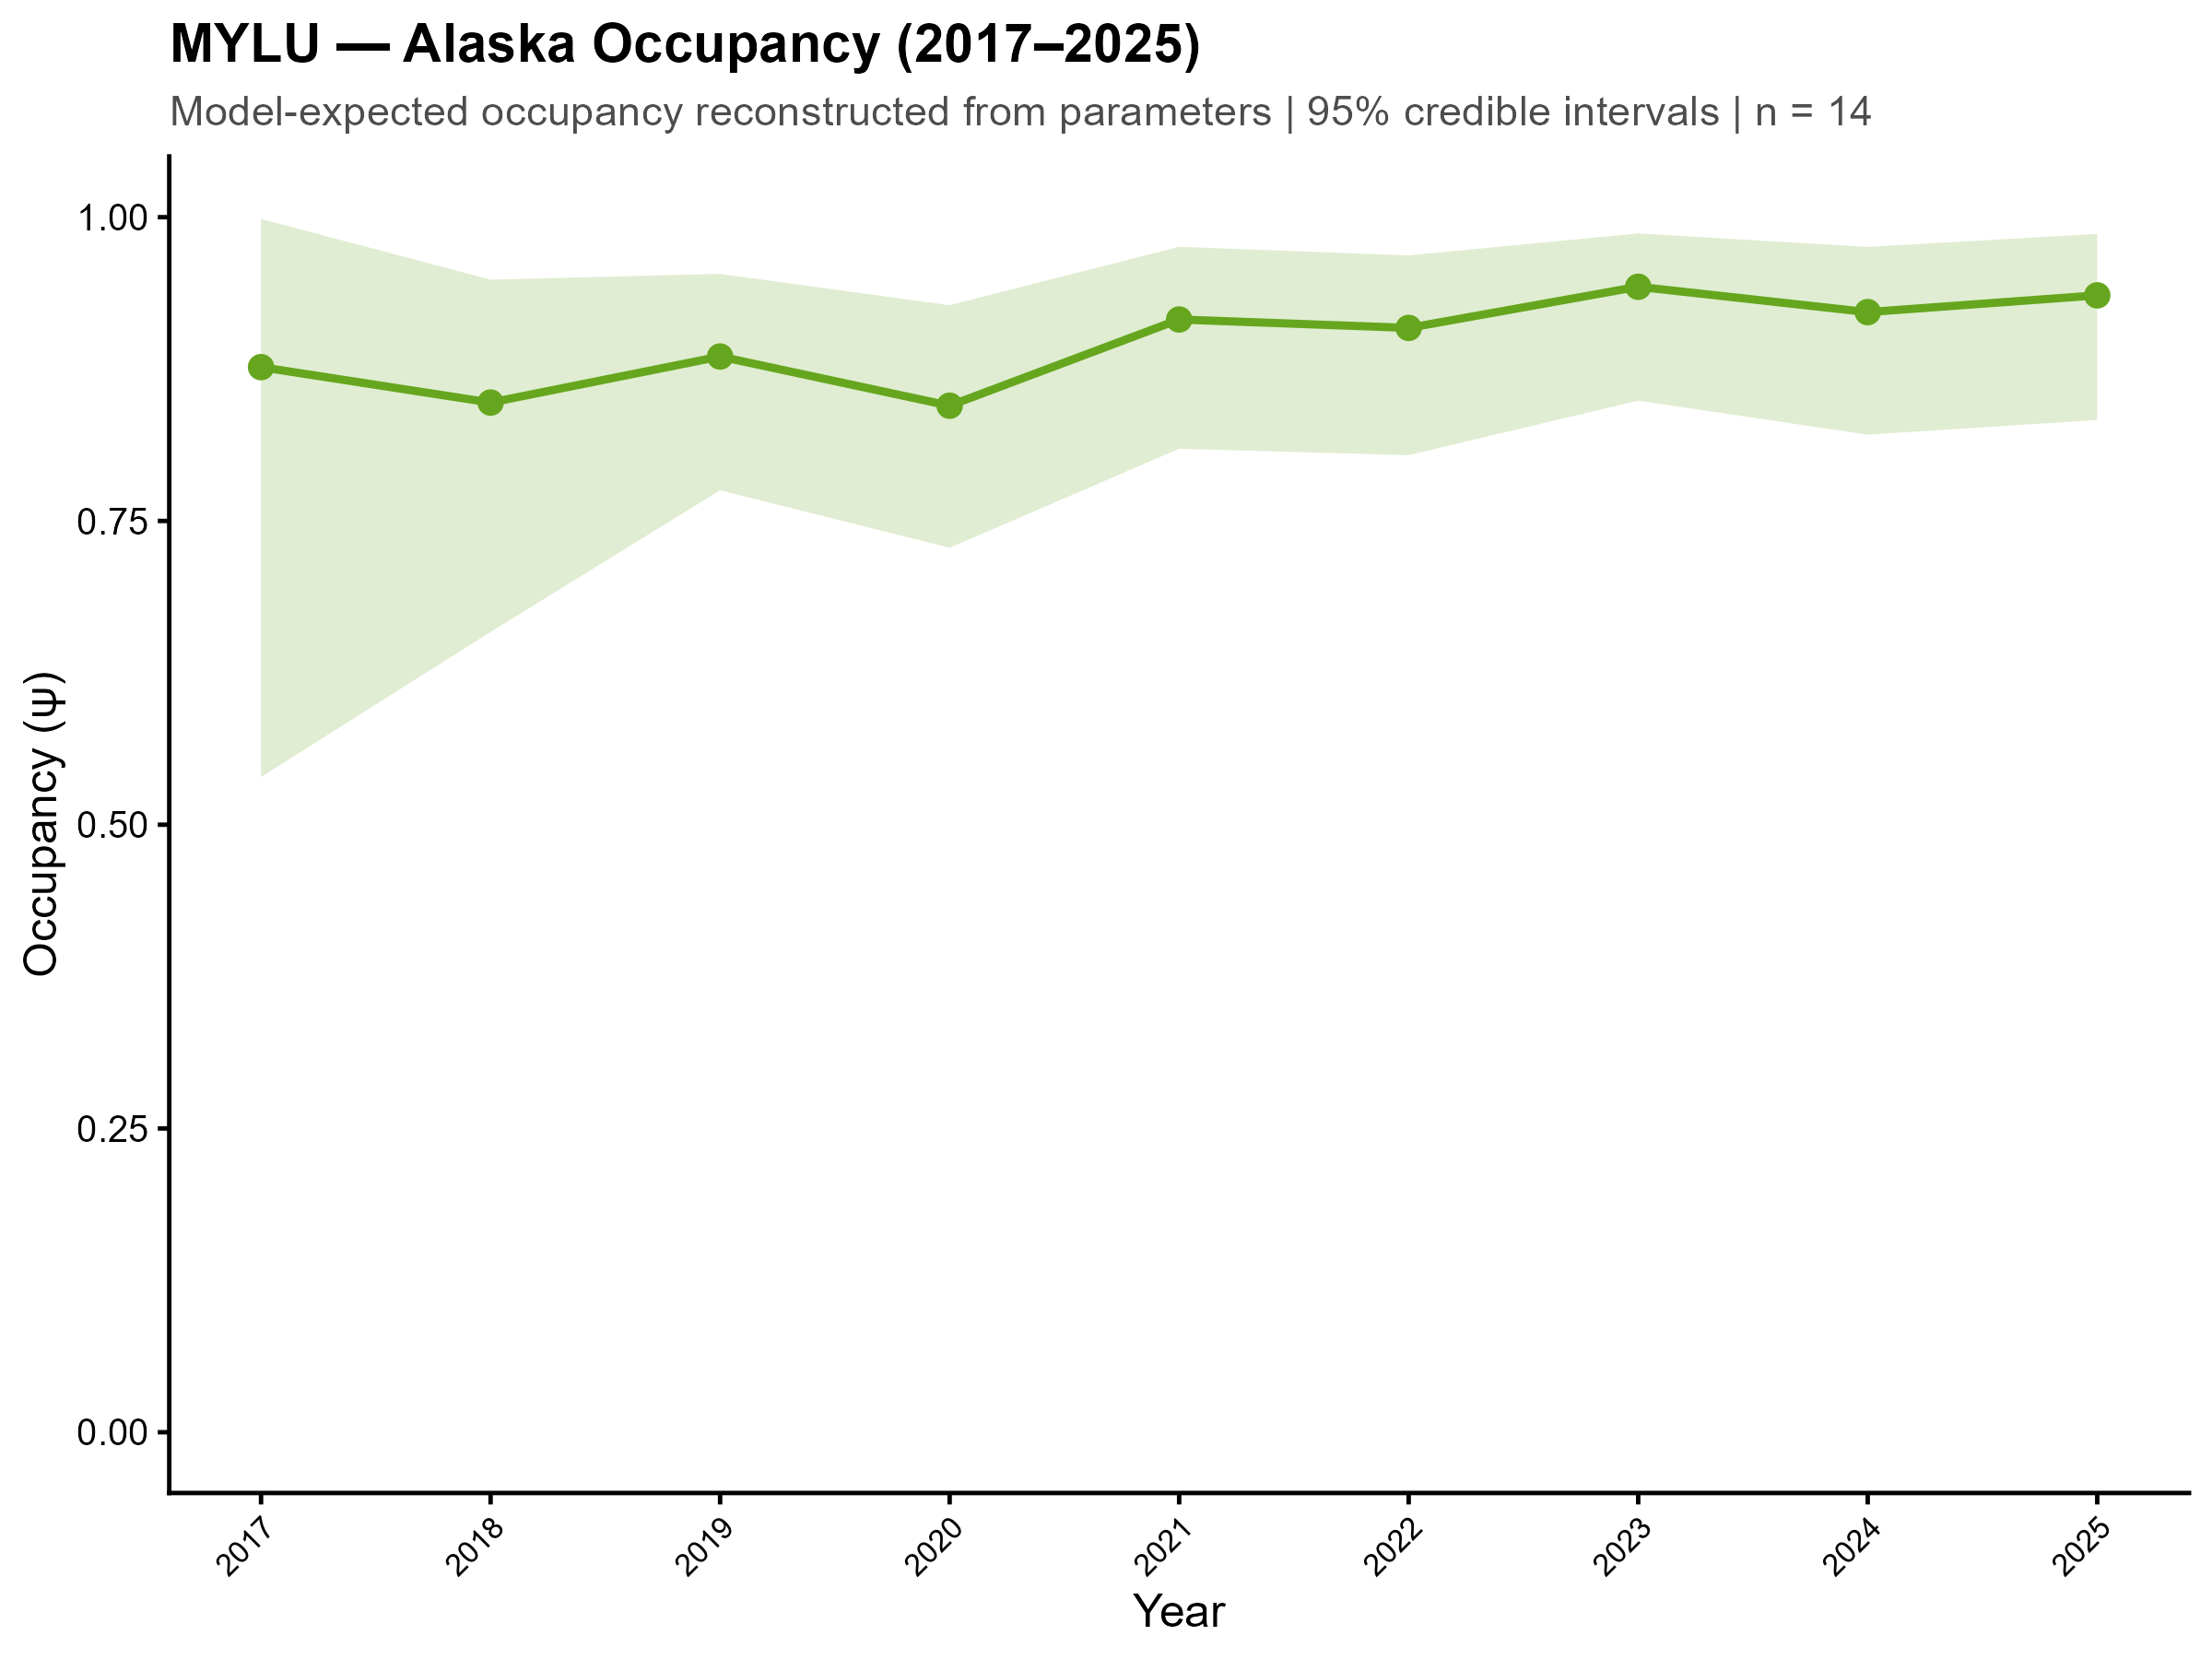
\includegraphics[keepaspectratio]{images/clipboard-3750373898.png}}
\pandocbounded{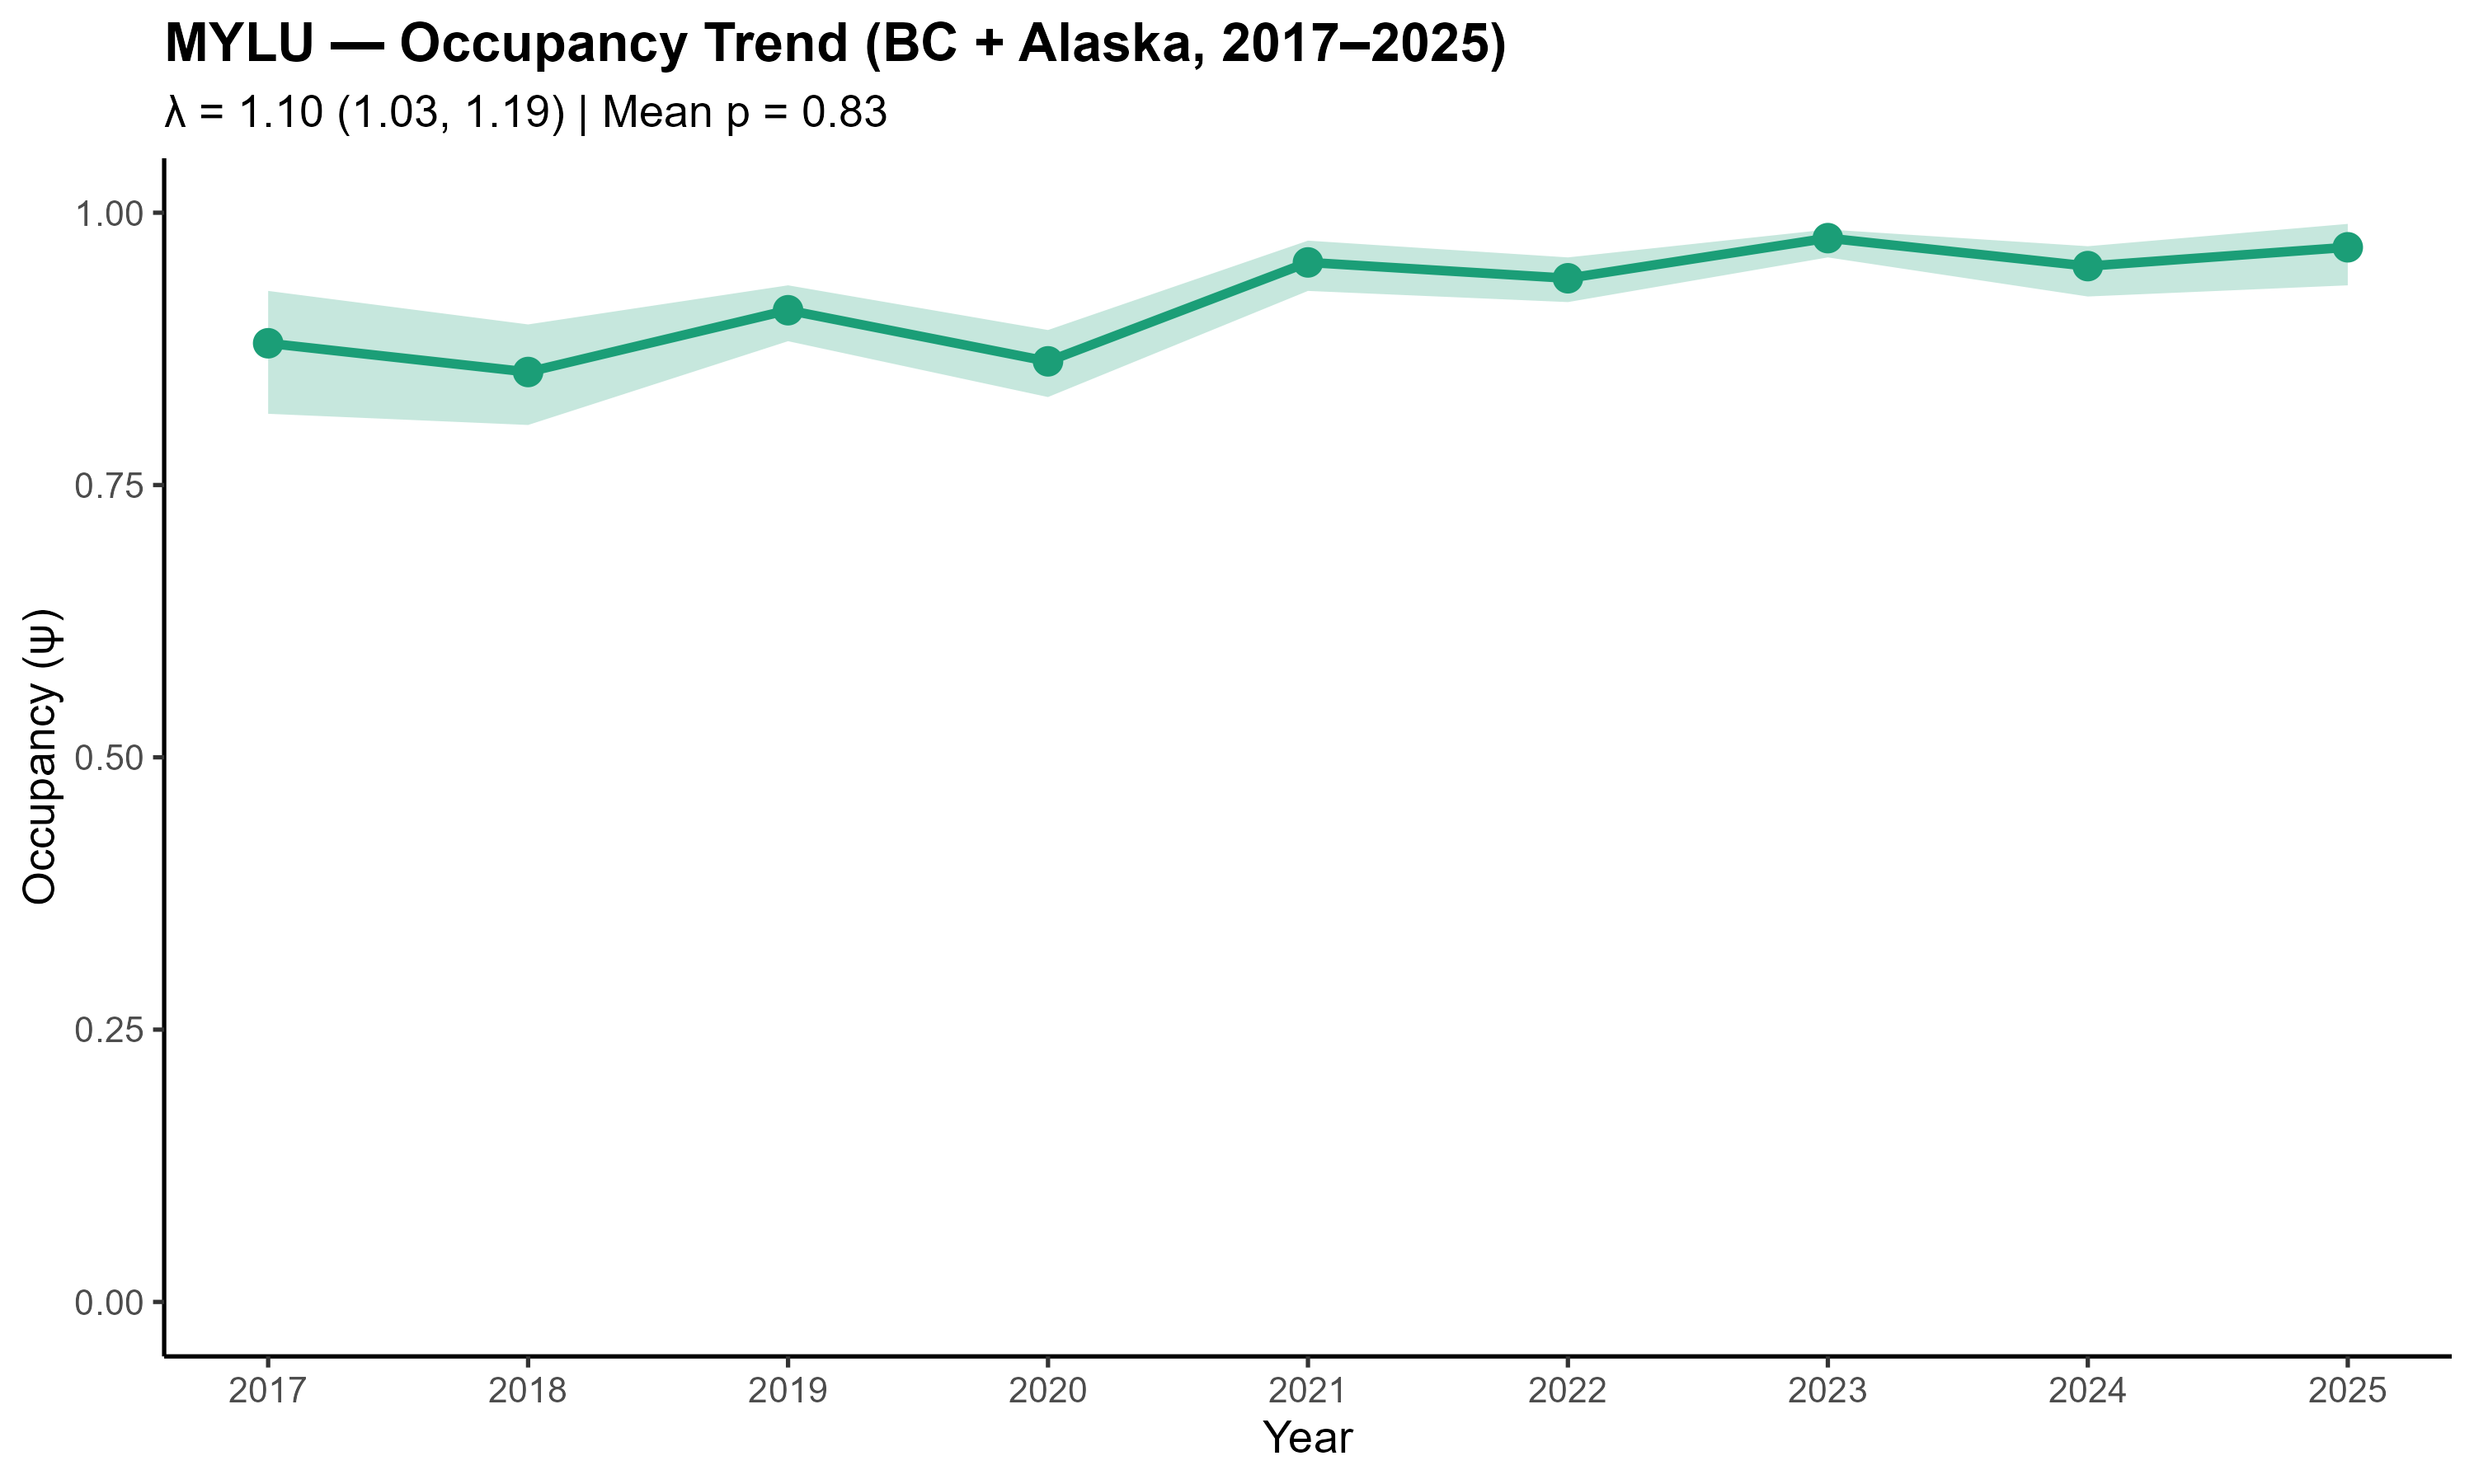
\includegraphics[keepaspectratio]{images/clipboard-2633679632.png}}
\pandocbounded{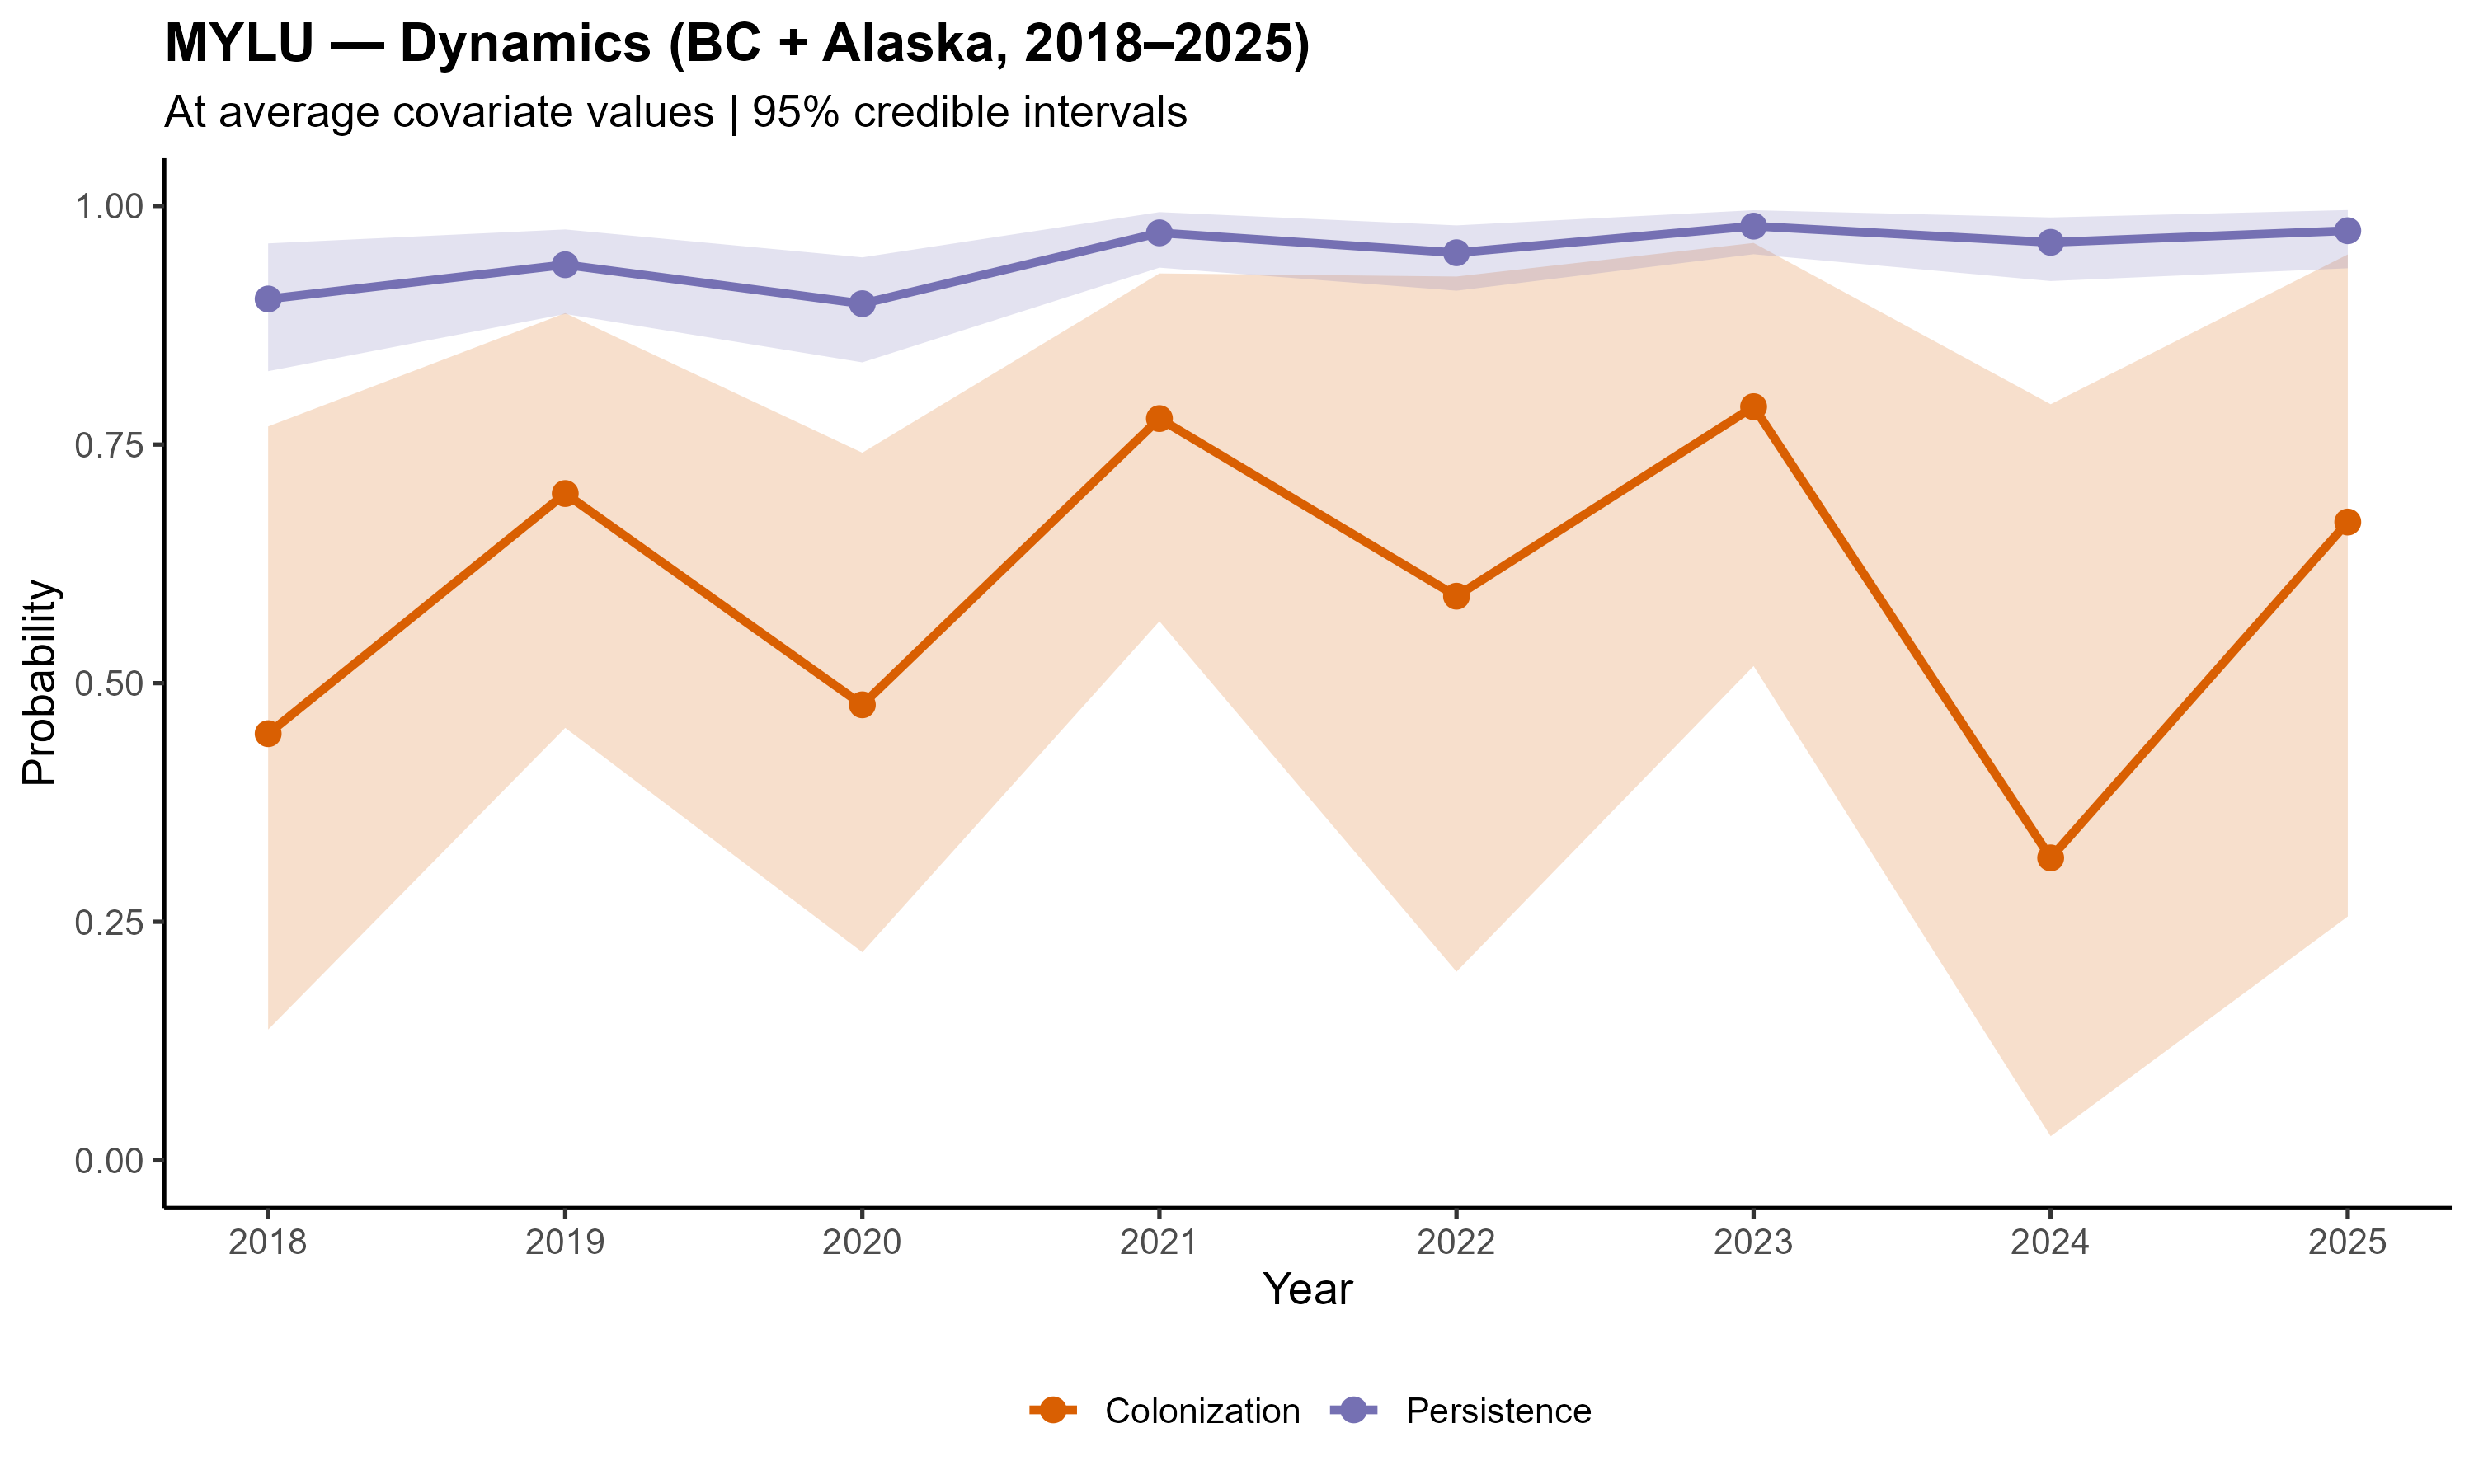
\includegraphics[keepaspectratio]{images/clipboard-2306693806.png}}
\pandocbounded{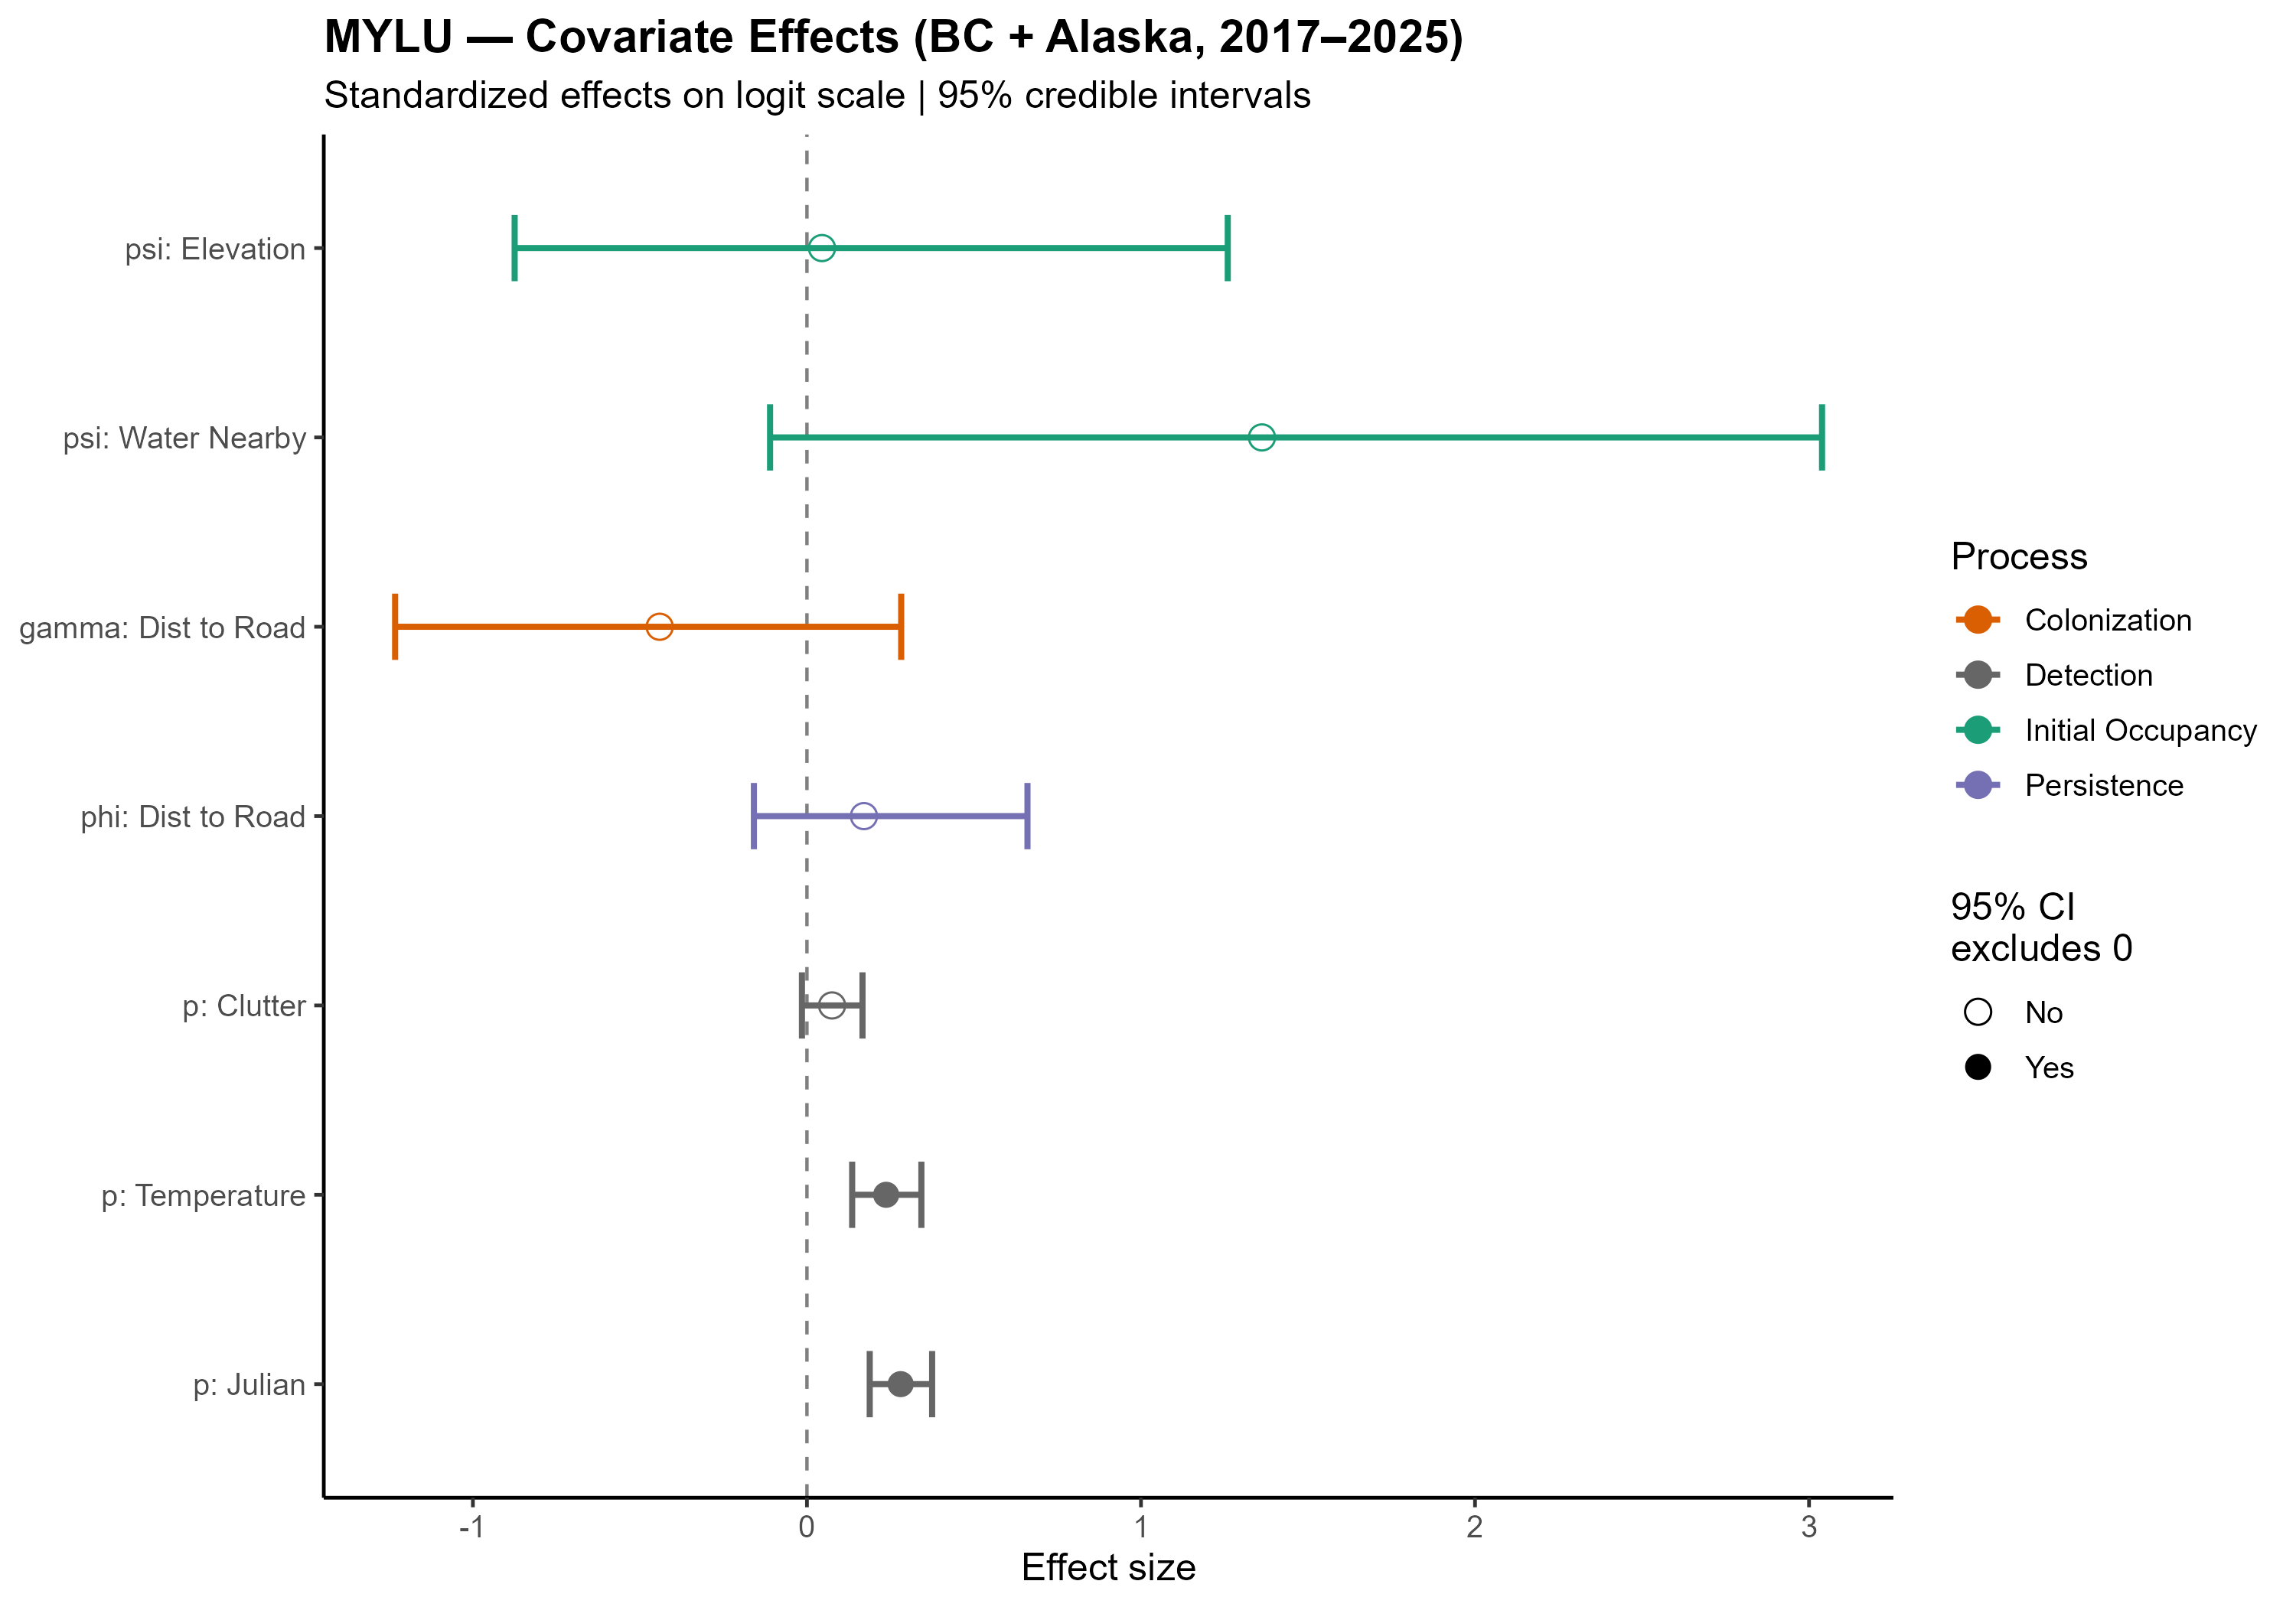
\includegraphics[keepaspectratio]{images/clipboard-79436506.png}}

\subsection{\texorpdfstring{Long-legged Myotis (\emph{Myotis
volans})}{Long-legged Myotis (Myotis volans)}}\label{long-legged-myotis-myotis-volans}

\pandocbounded{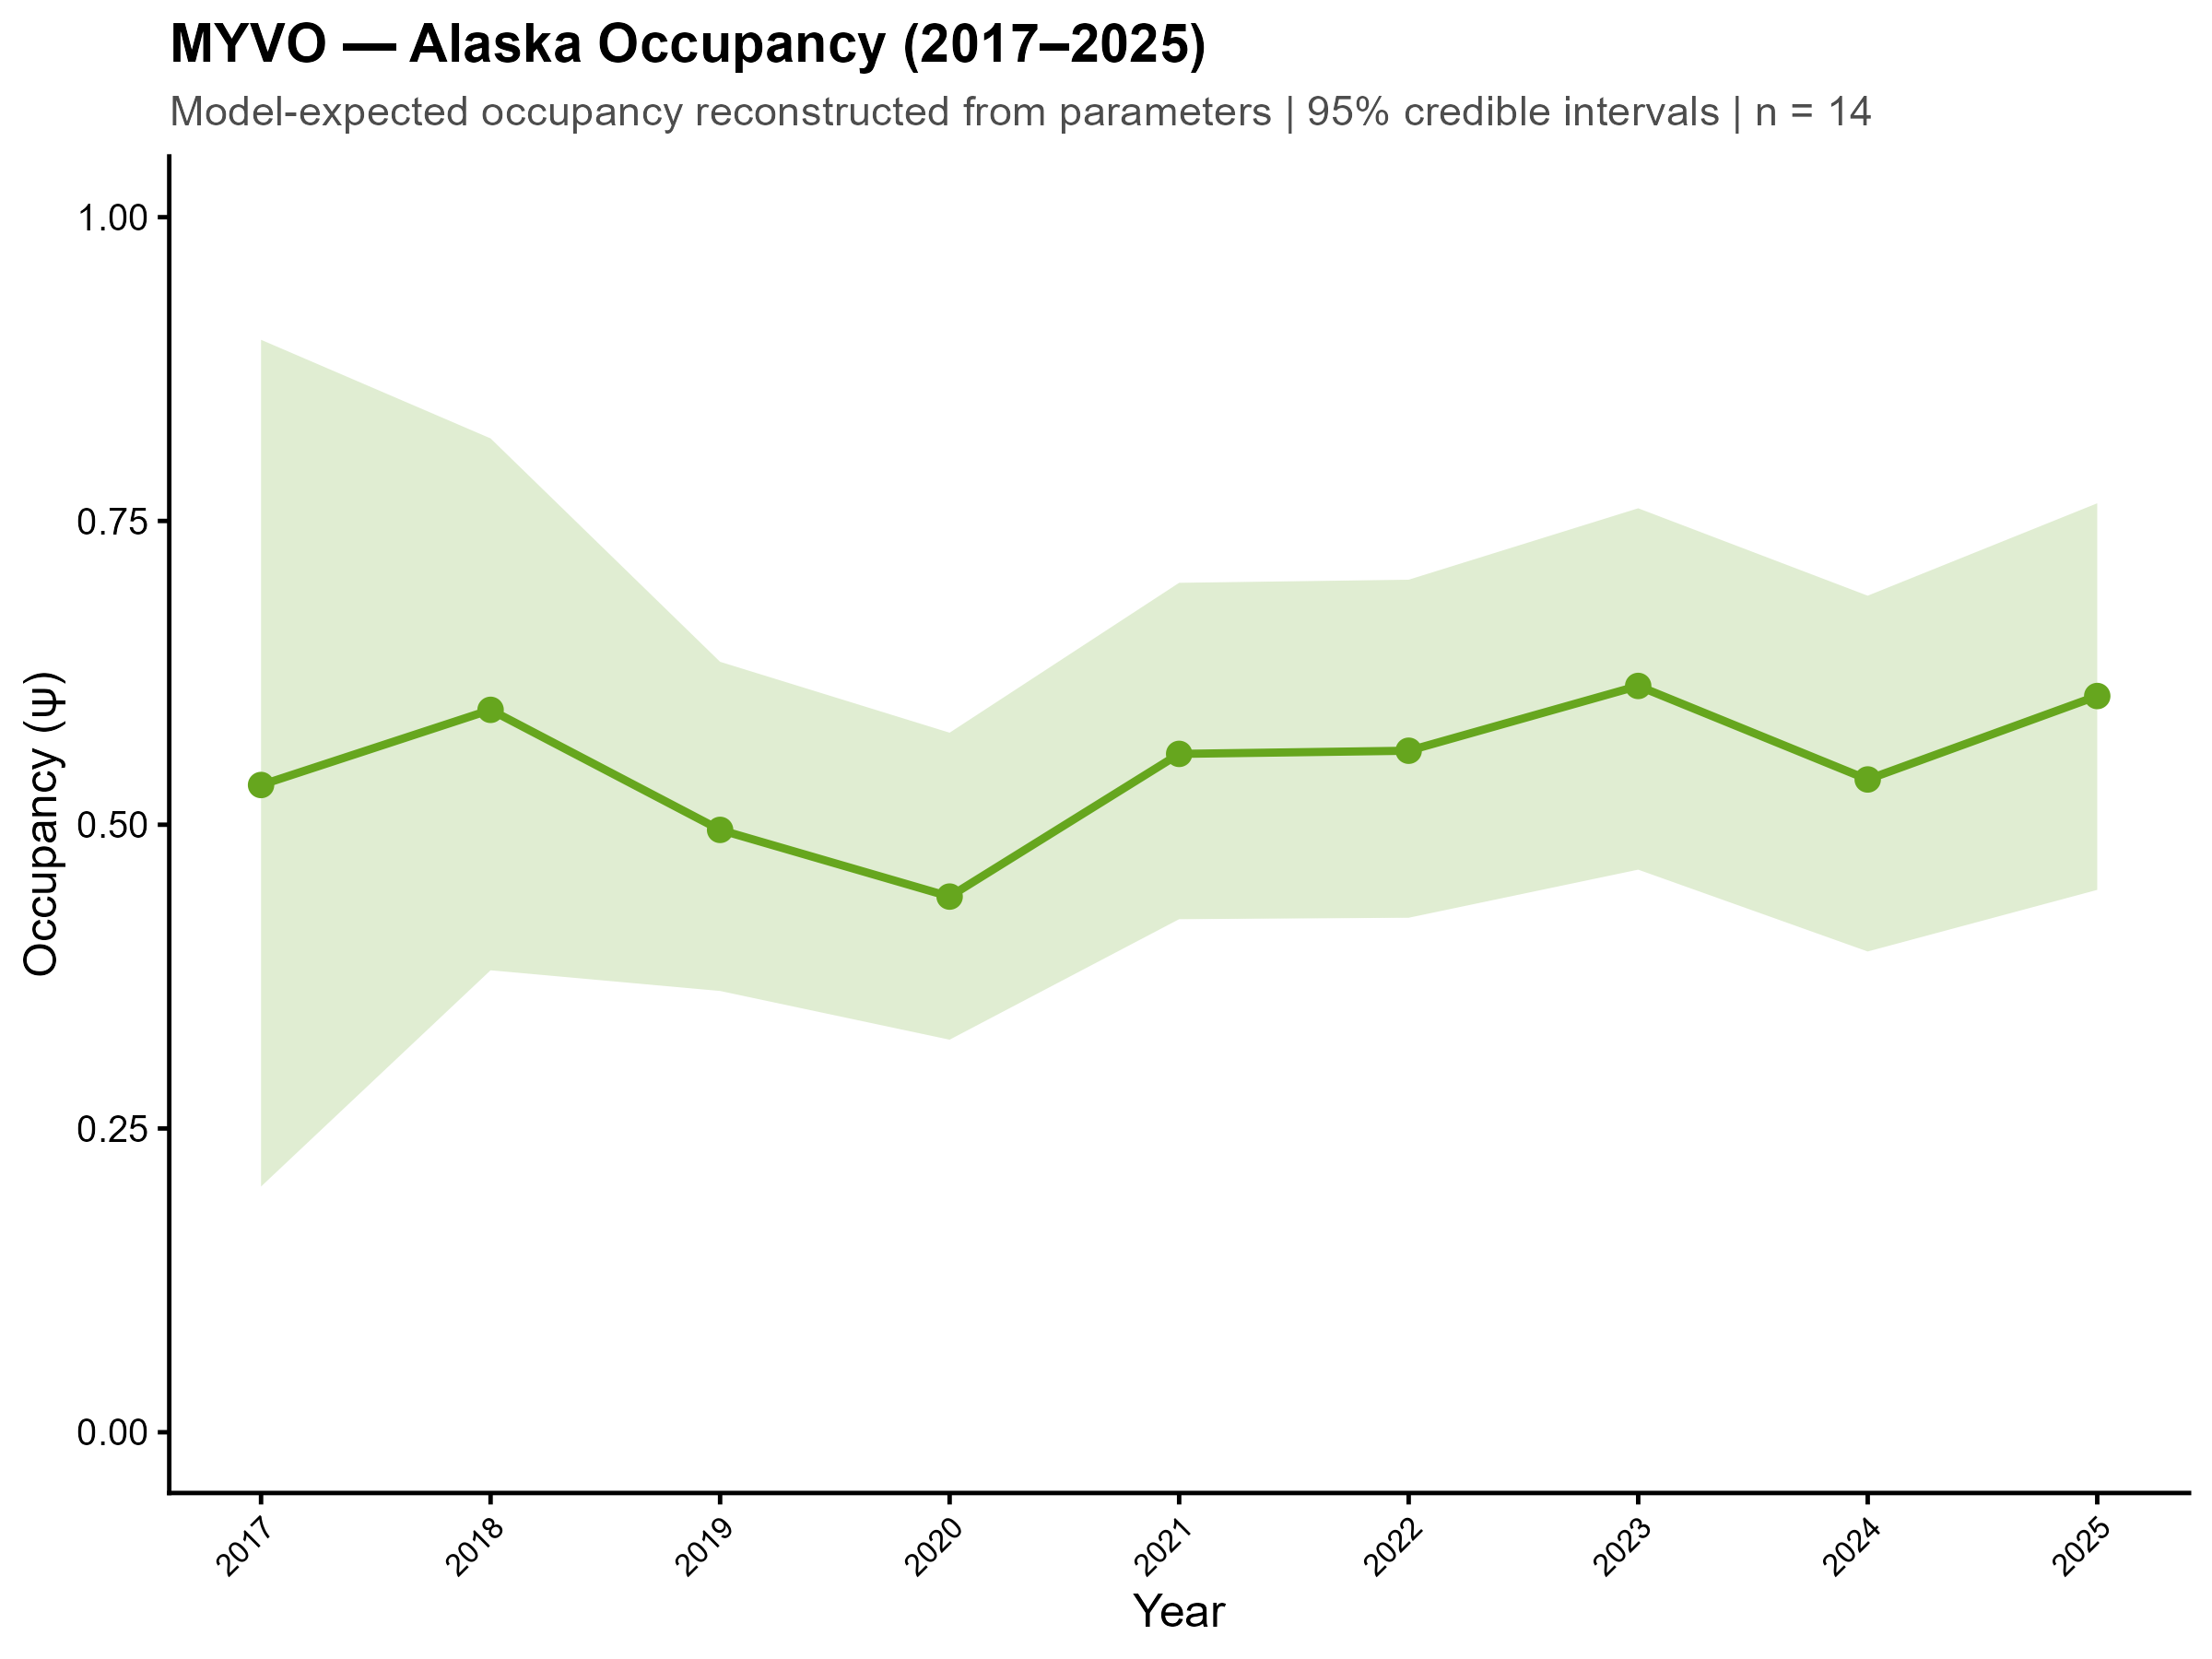
\includegraphics[keepaspectratio]{images/clipboard-378845605.png}}
\pandocbounded{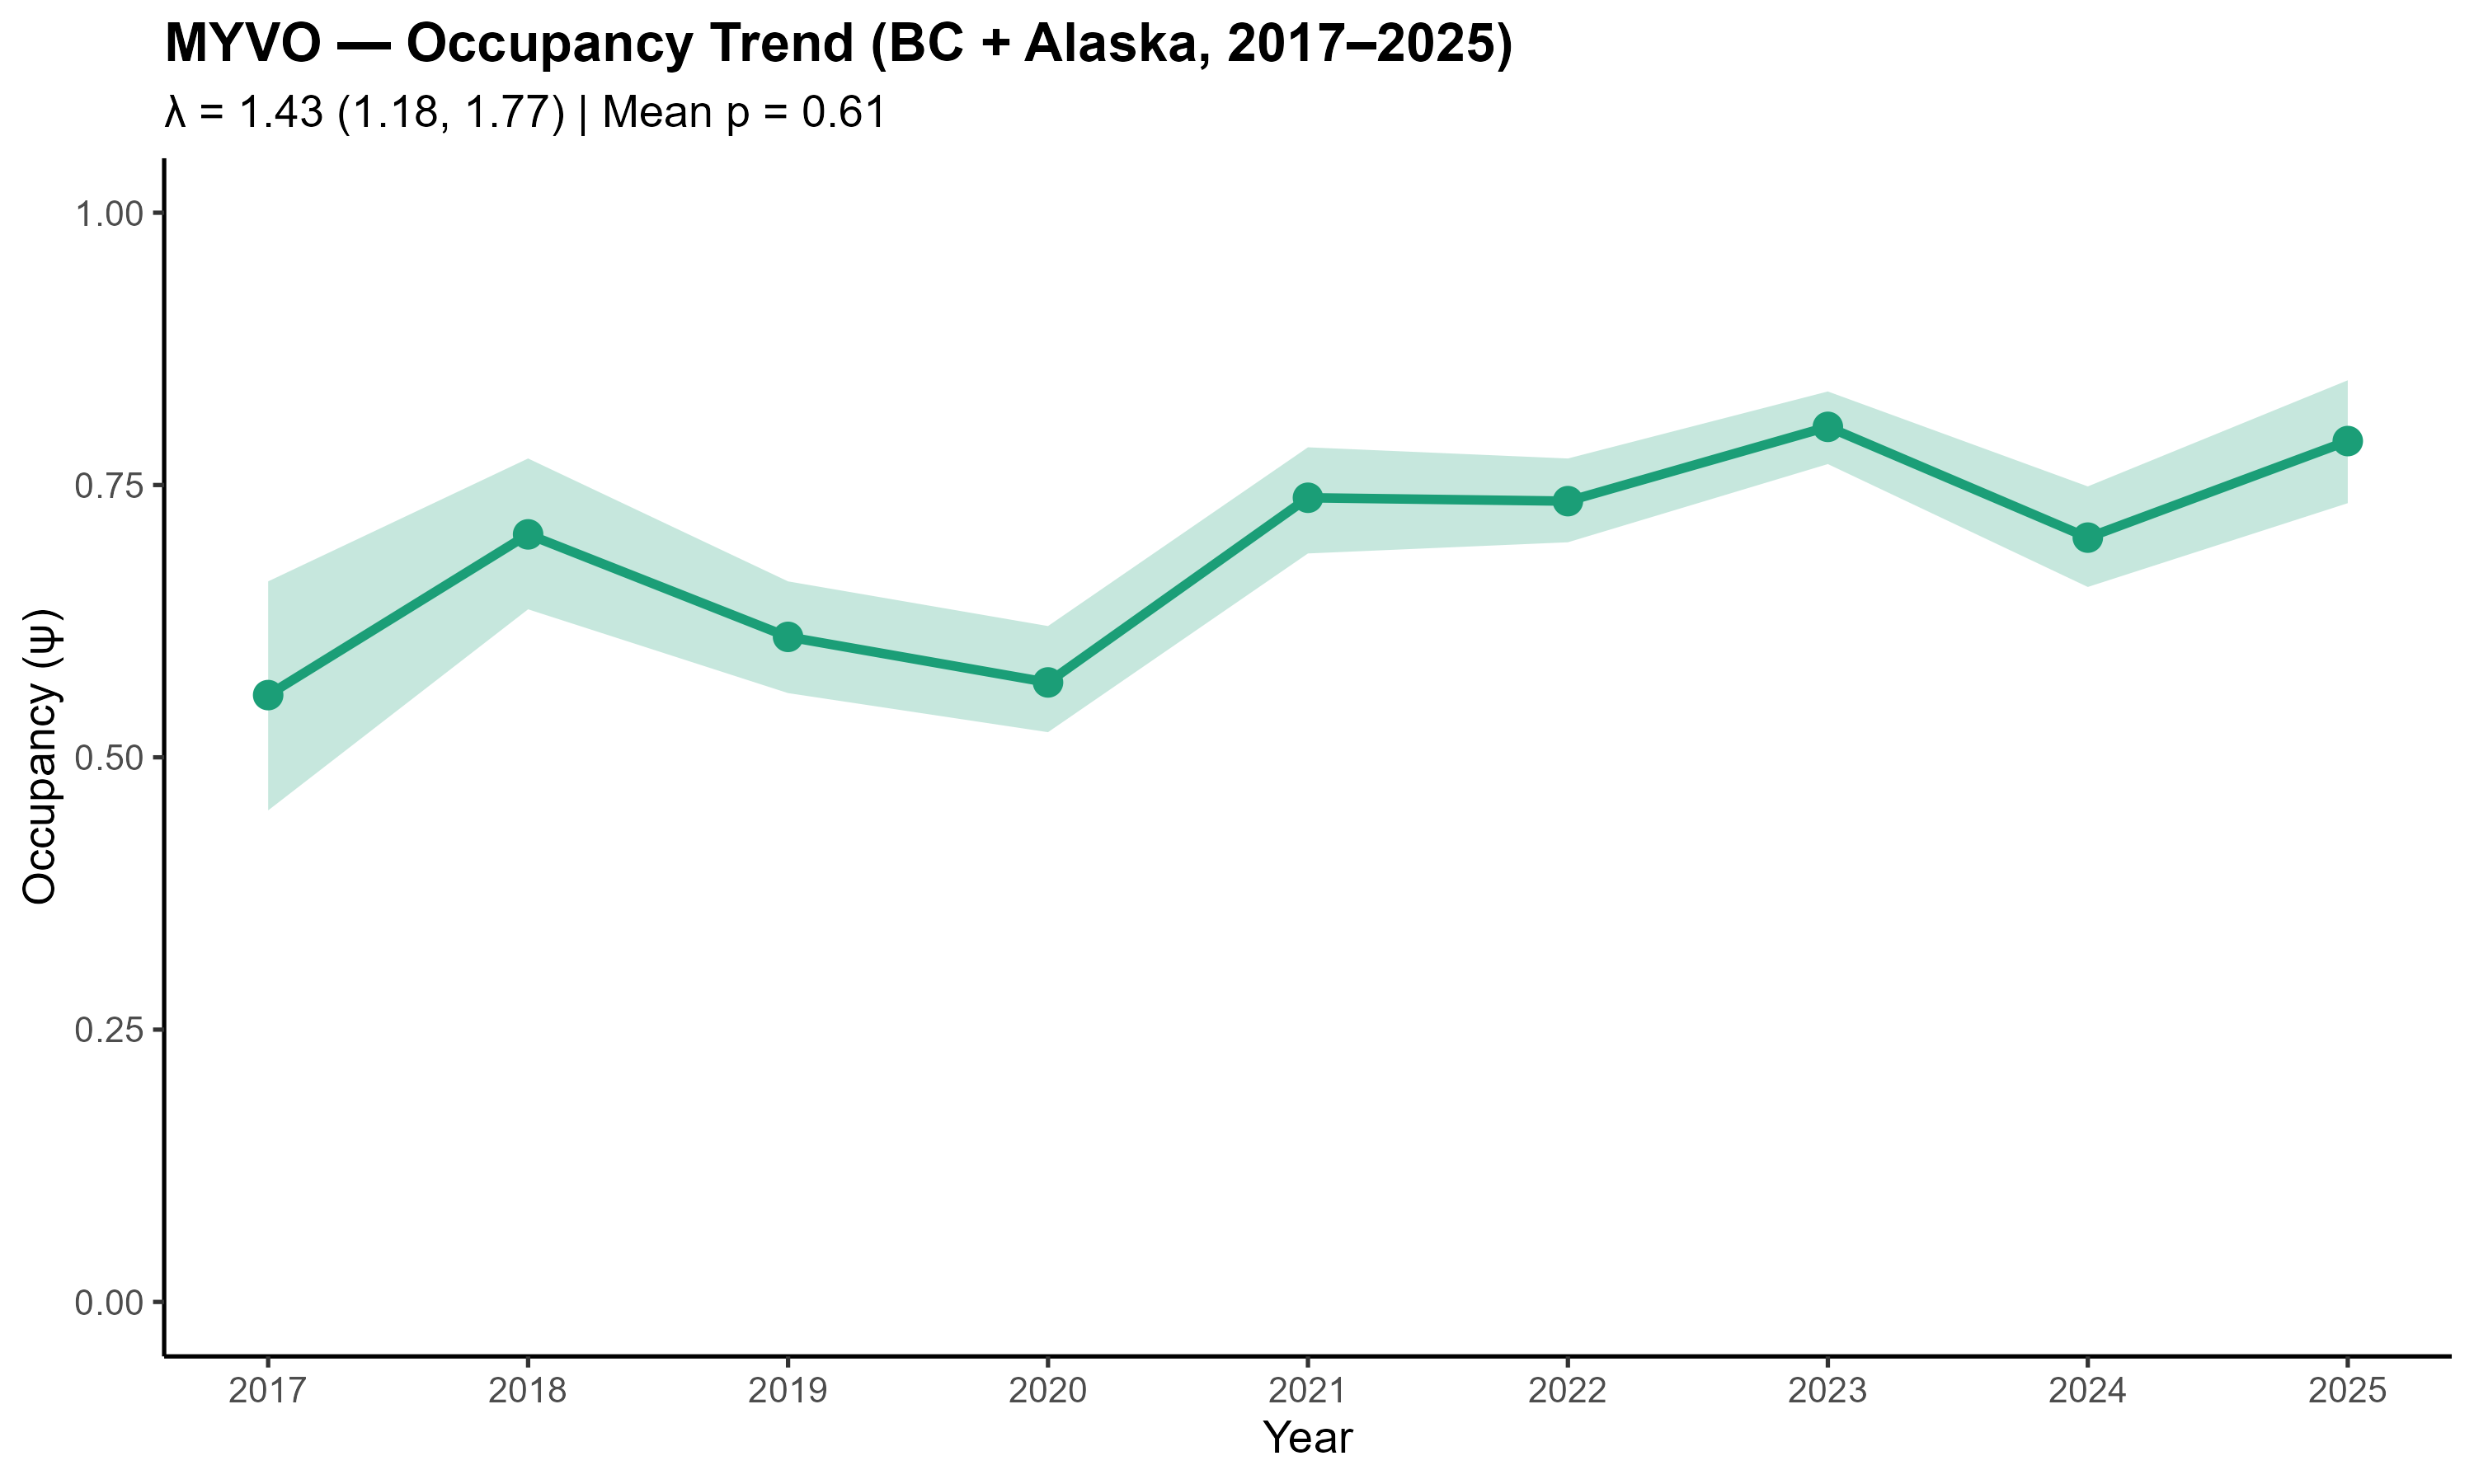
\includegraphics[keepaspectratio]{images/clipboard-2874082935.png}}
\pandocbounded{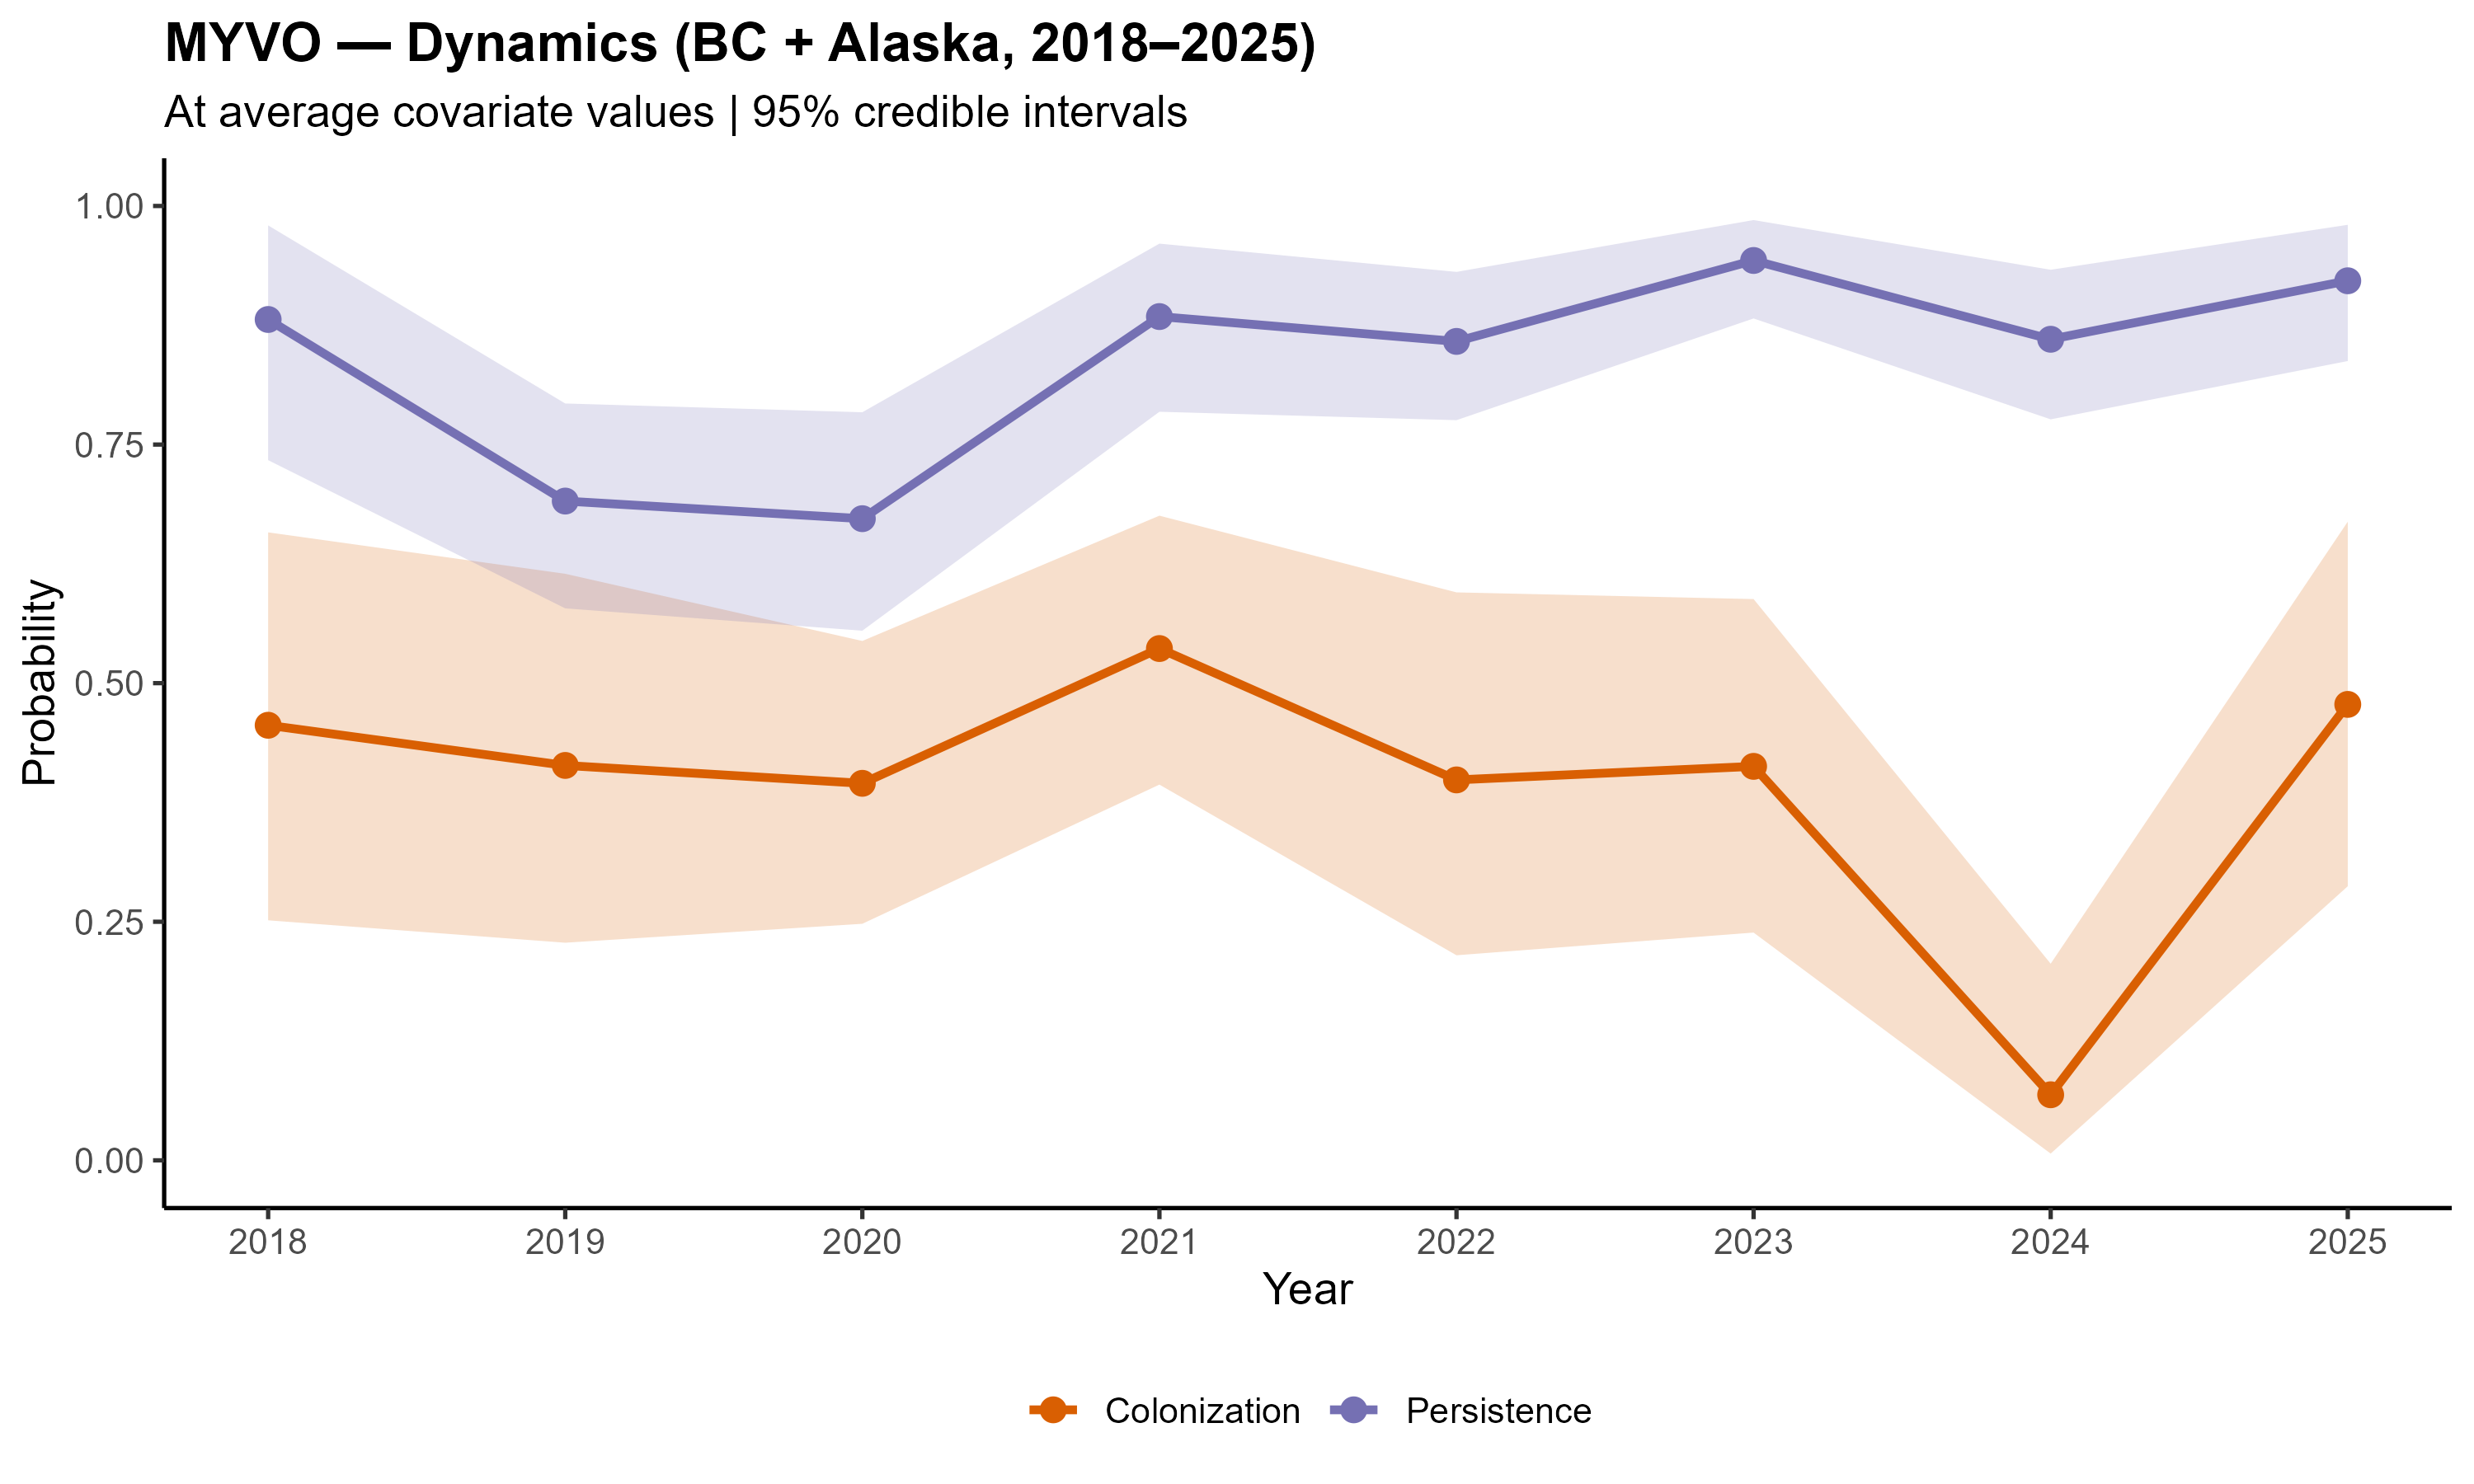
\includegraphics[keepaspectratio]{images/clipboard-2053734589.png}}
\pandocbounded{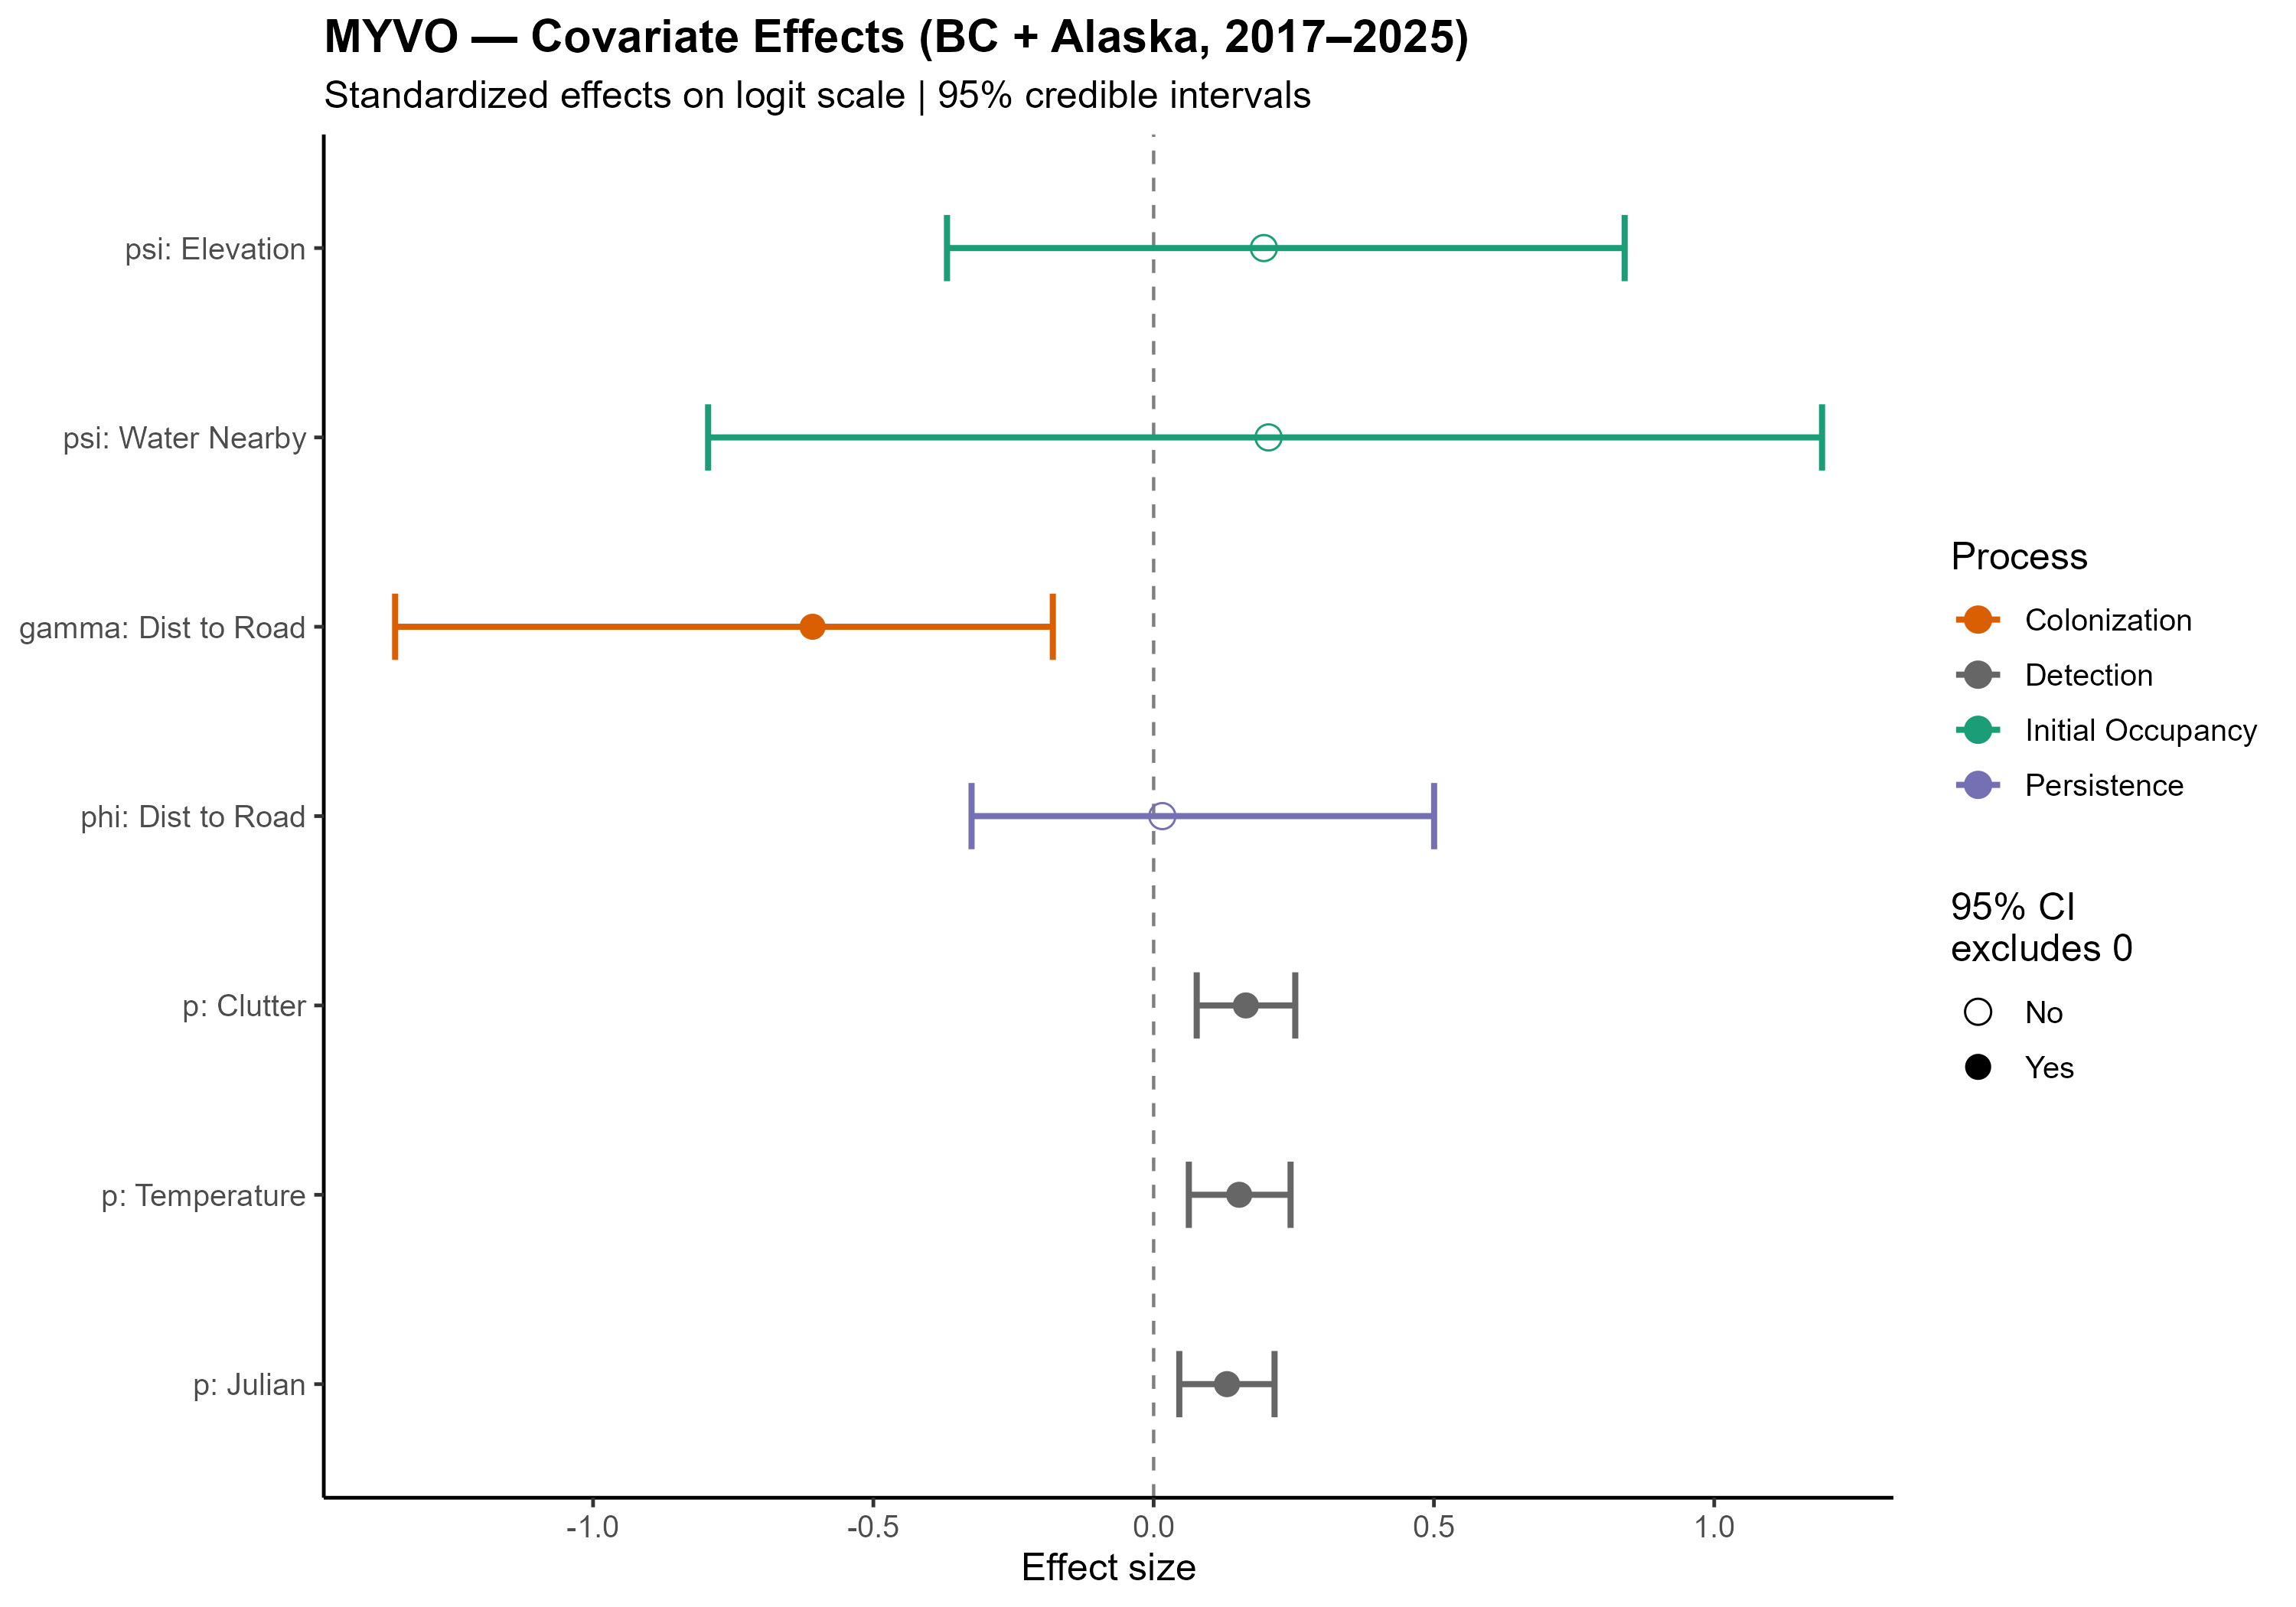
\includegraphics[keepaspectratio]{images/clipboard-4053125643.png}}

\newpage{}

\section{Appendix B}\label{appendix-b}

Species detection summaries by GRTS cell. For each cell, 2025 plots
appear first, with the 2024 equivalents below where the cell was sampled
in 2024.

\subsection*{Grid cell 206 - POW}\label{grid-cell-206---pow}

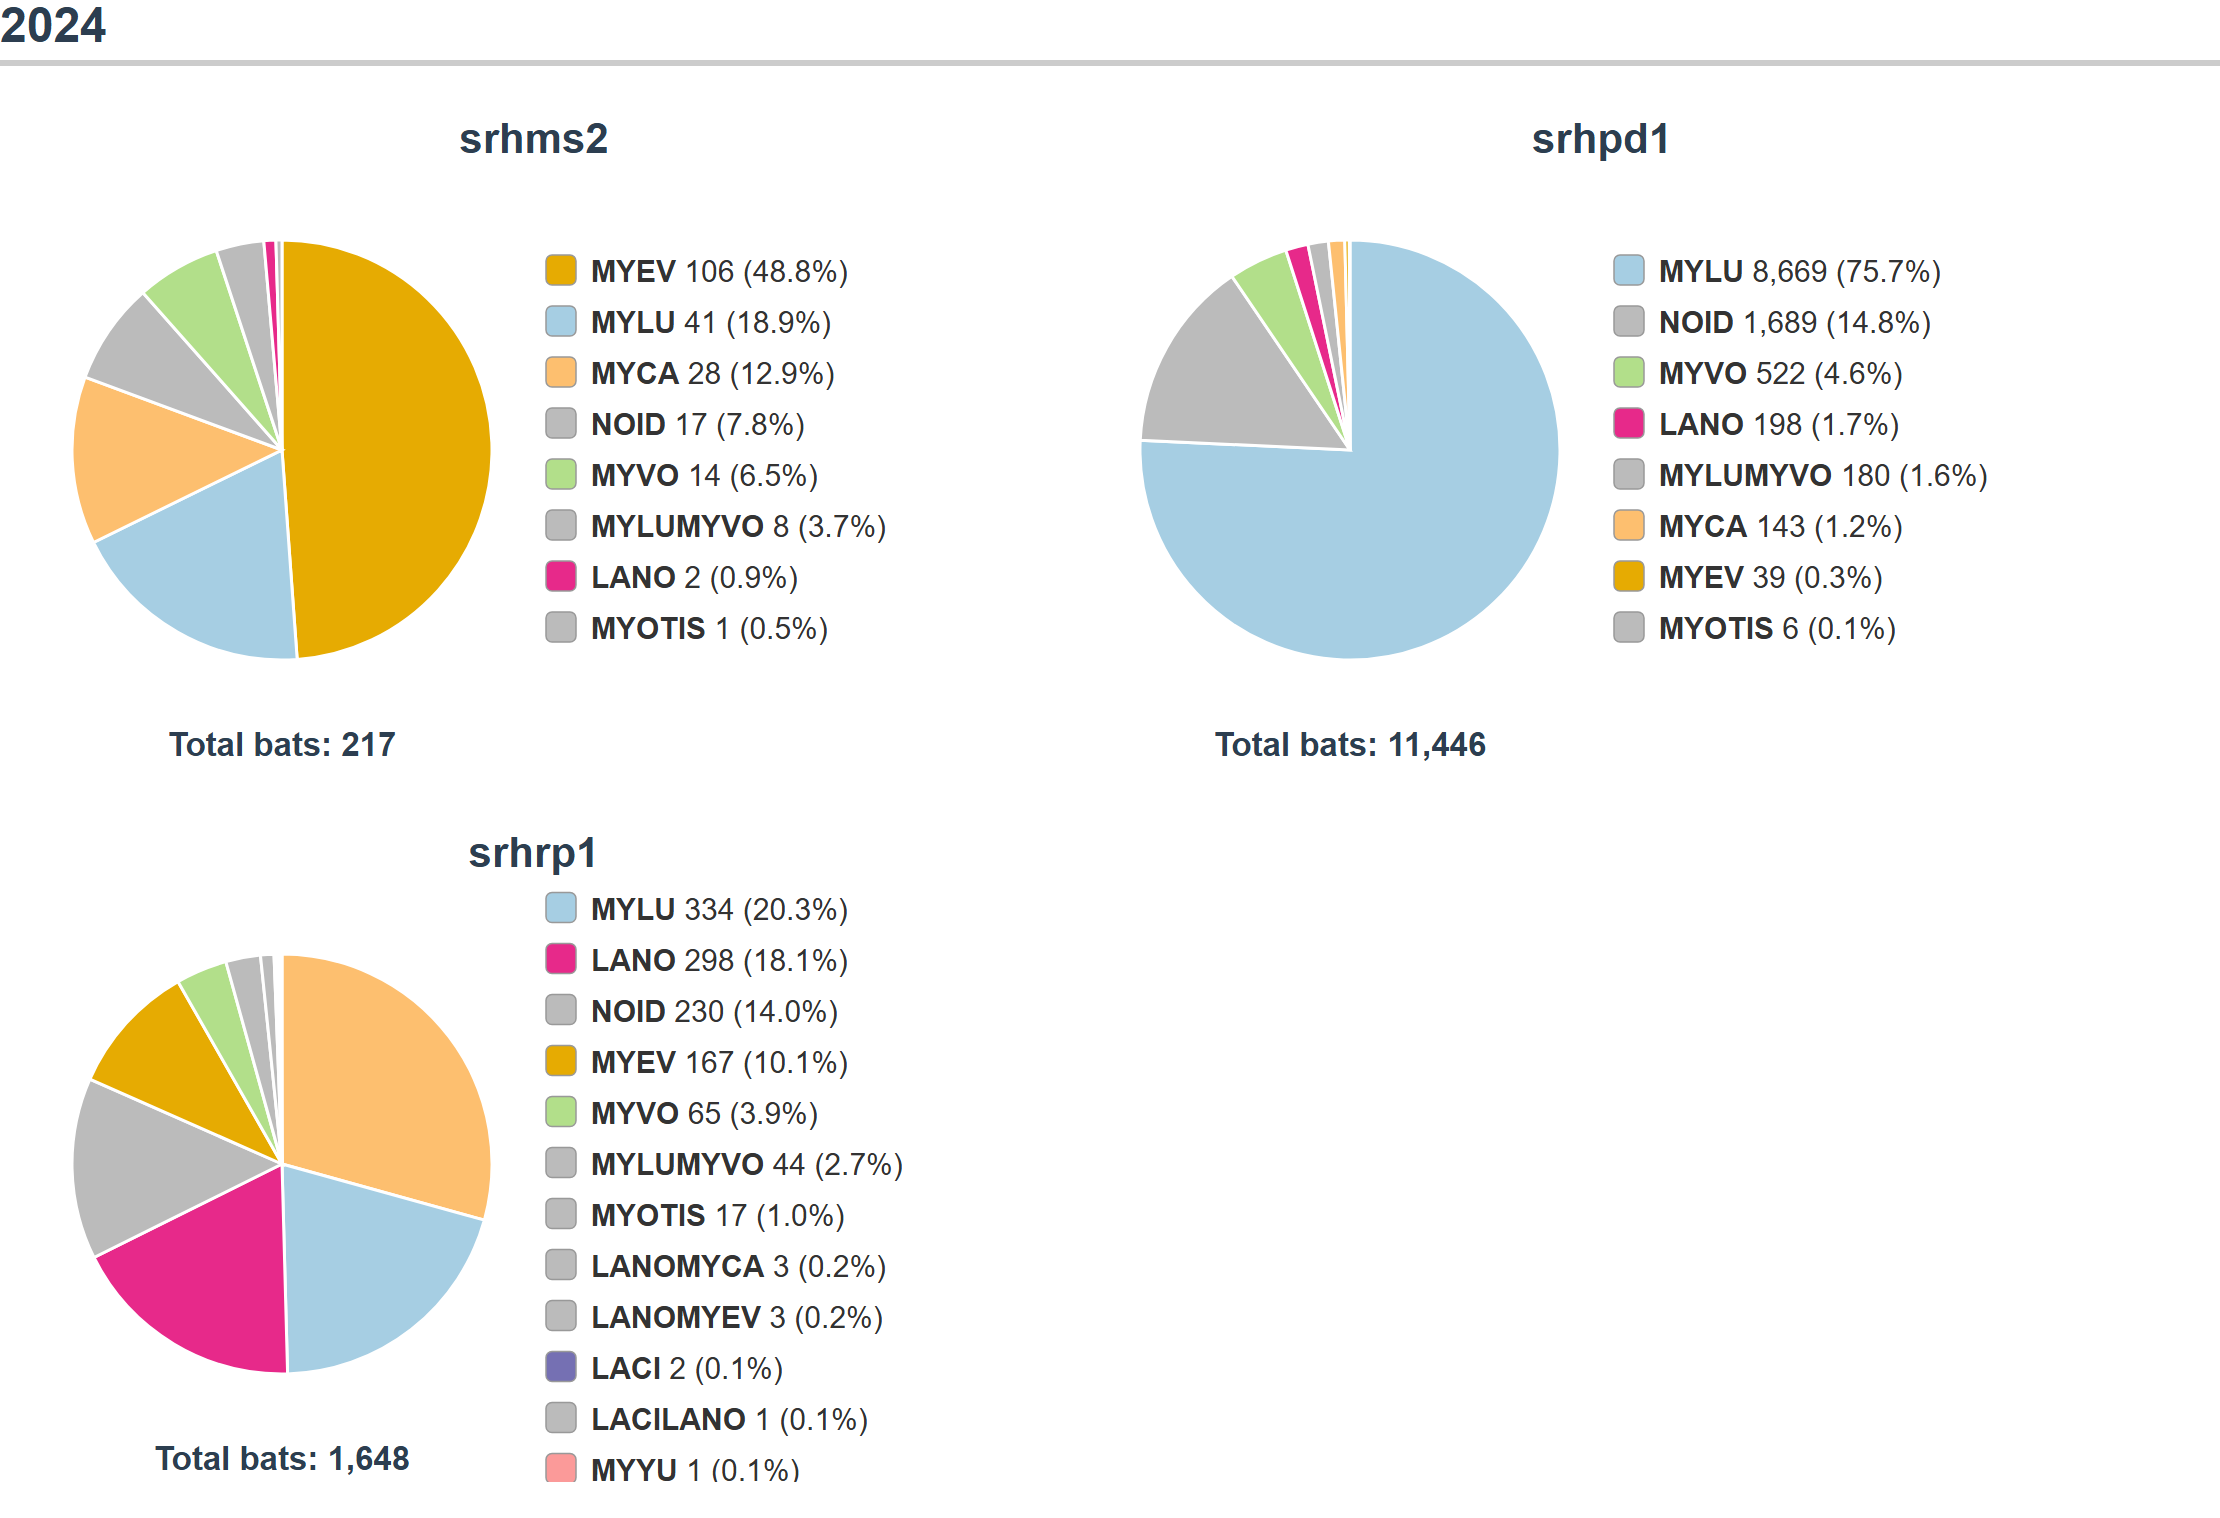
\includegraphics[width=1\linewidth,height=\textheight,keepaspectratio]{Figures/AppendixB/206_pies.png}

\newpage

\begin{figure}[H]

{\centering 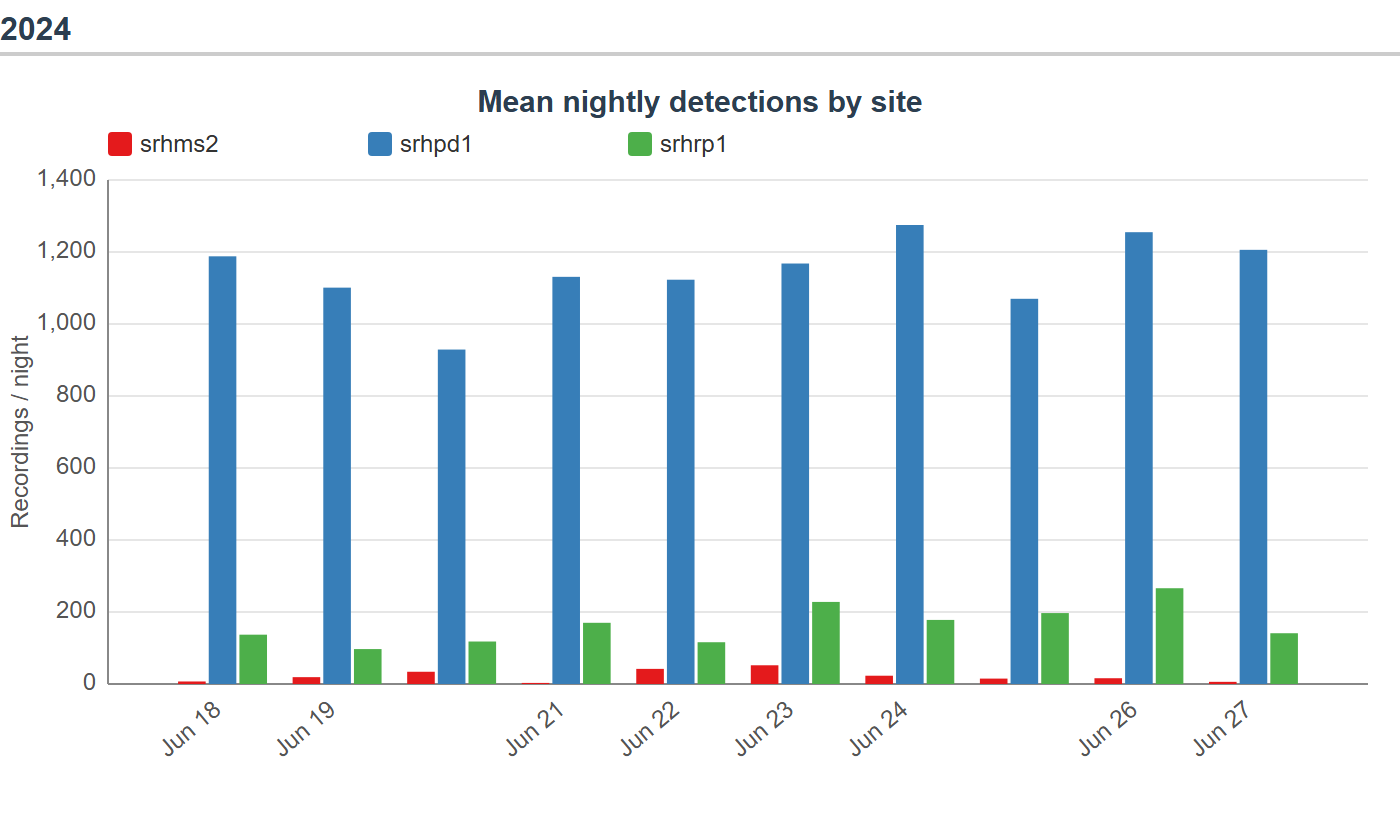
\includegraphics[width=1\linewidth,height=\textheight,keepaspectratio]{Figures/AppendixB/206_bar.png}

}

\caption{Nightly activity by site (2025 top, 2024 below), cell 206 -
POW}

\end{figure}%

\newpage

\begin{figure}[H]

{\centering 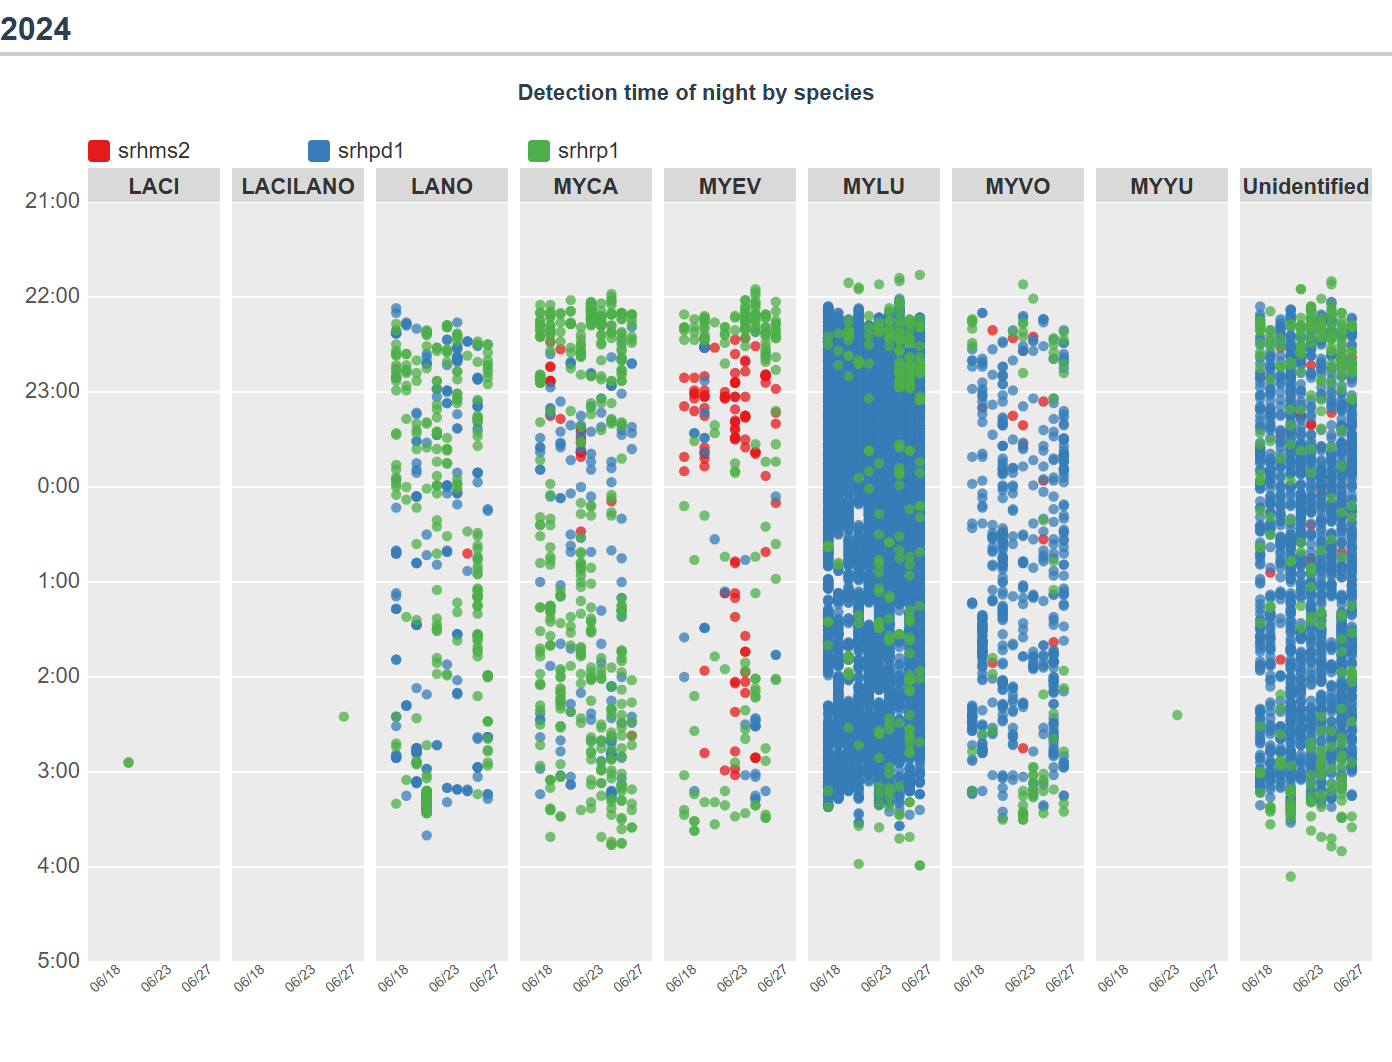
\includegraphics[width=1\linewidth,height=\textheight,keepaspectratio]{Figures/AppendixB/206_hour.png}

}

\caption{Detection times by species and site (2025 top, 2024 below),
cell 206 - POW}

\end{figure}%

\newpage

\subsection*{Grid cell 5006 -
Petersburg}\label{grid-cell-5006---petersburg}

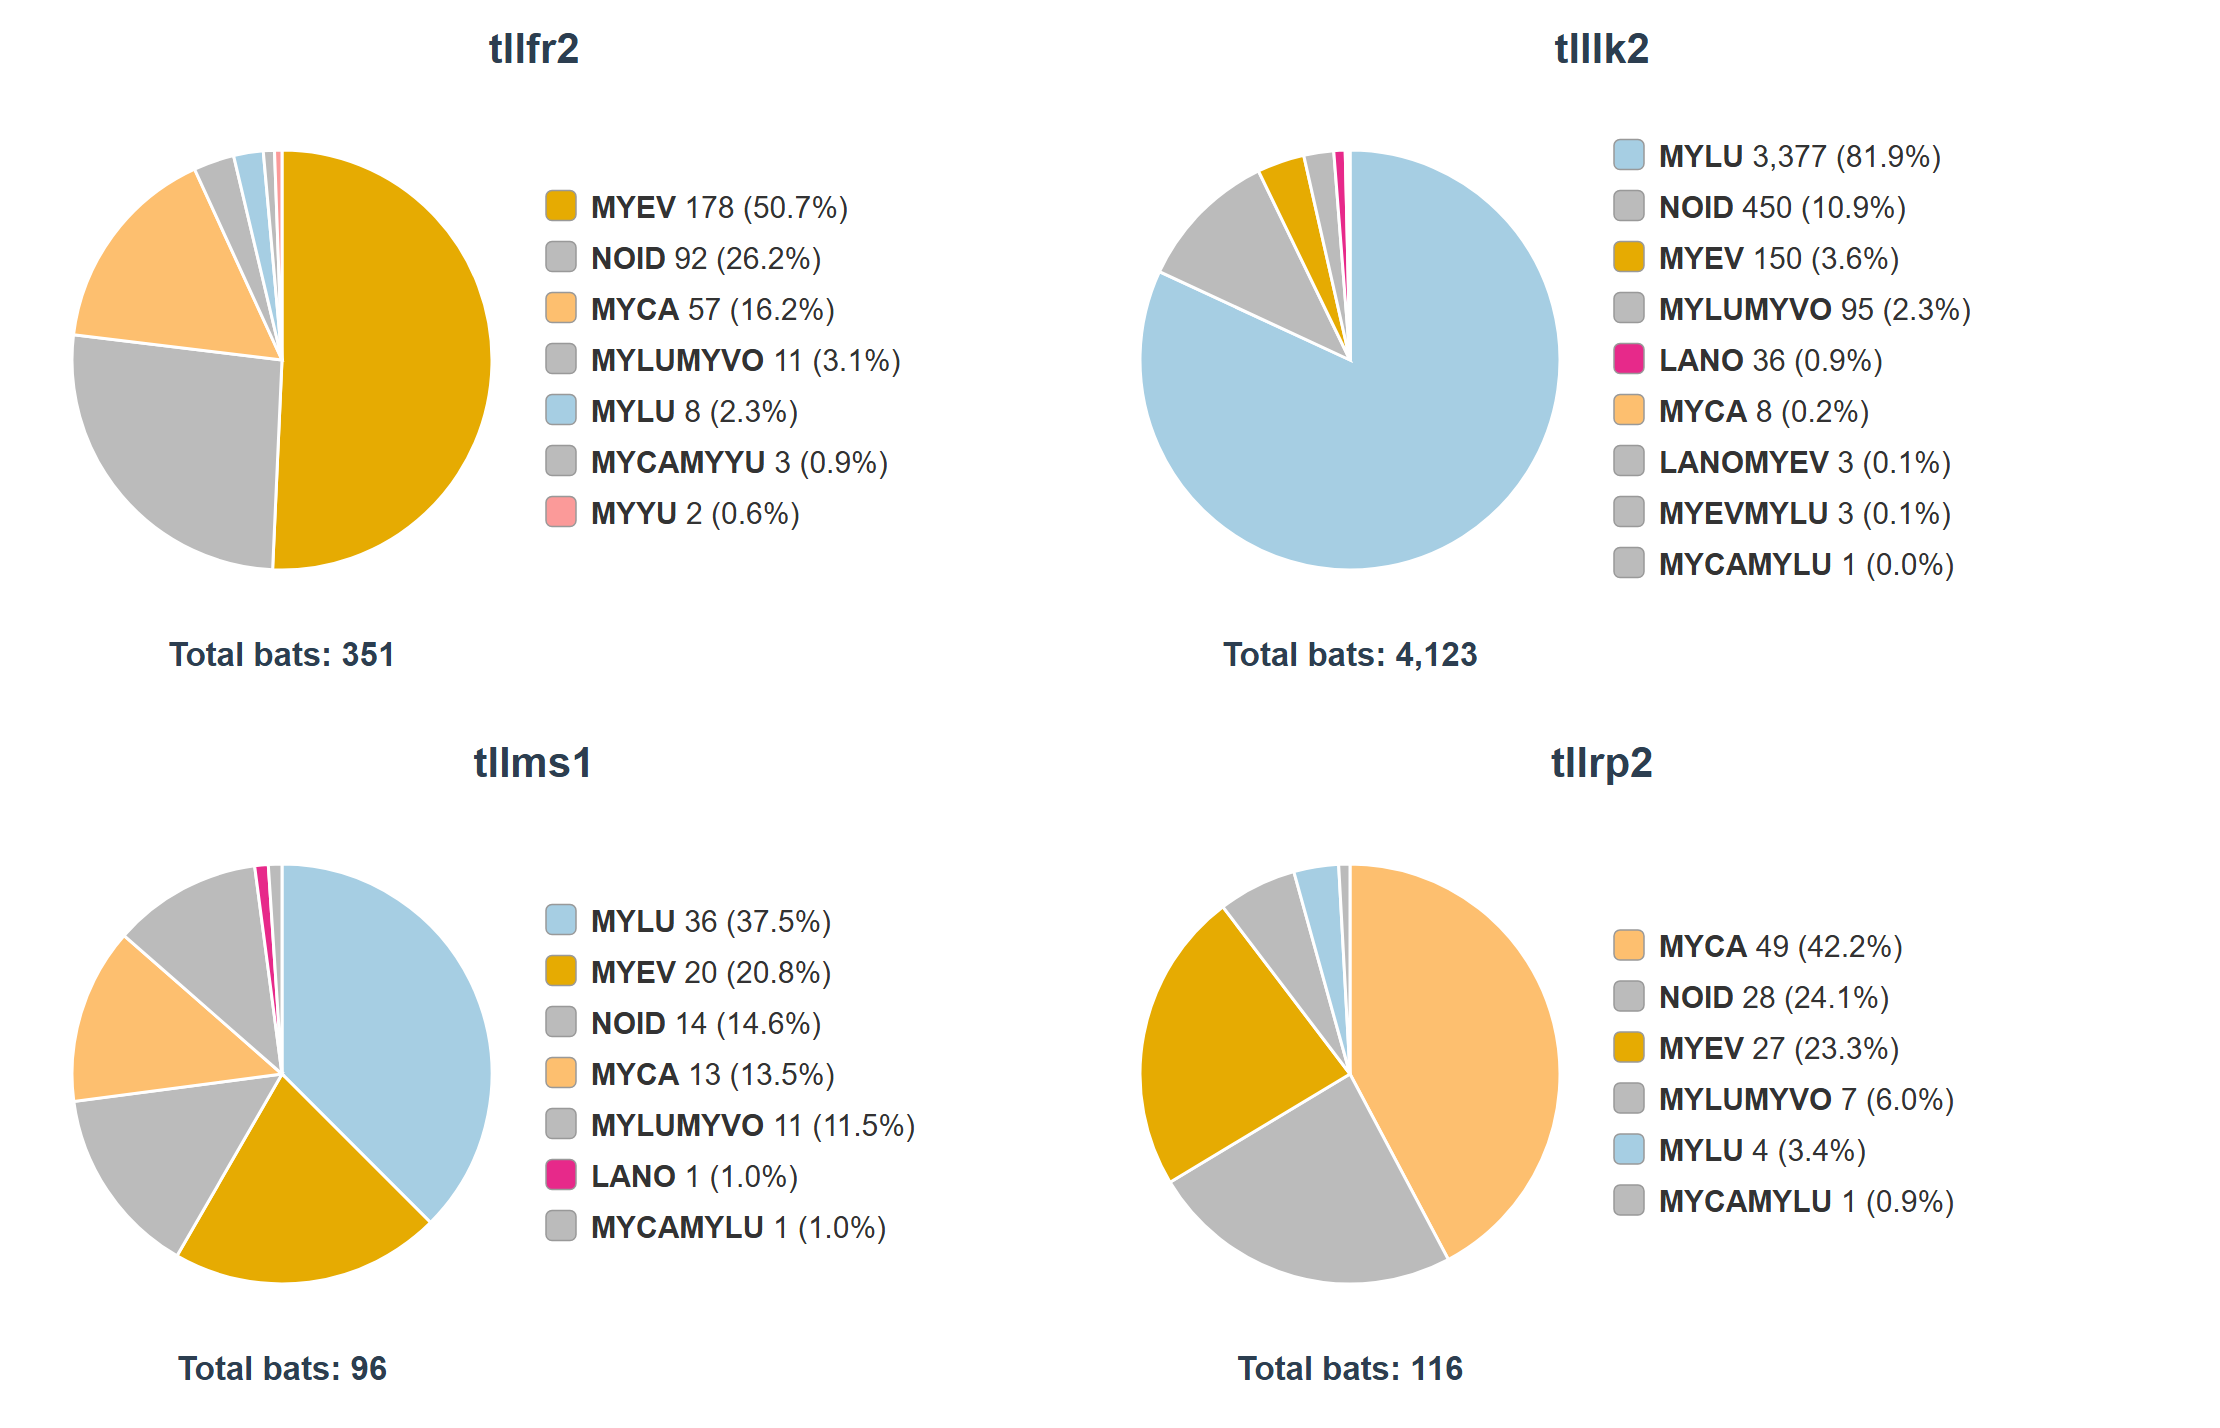
\includegraphics[width=1\linewidth,height=\textheight,keepaspectratio]{Figures/AppendixB/5006_pies.png}

\newpage

\begin{figure}[H]

{\centering 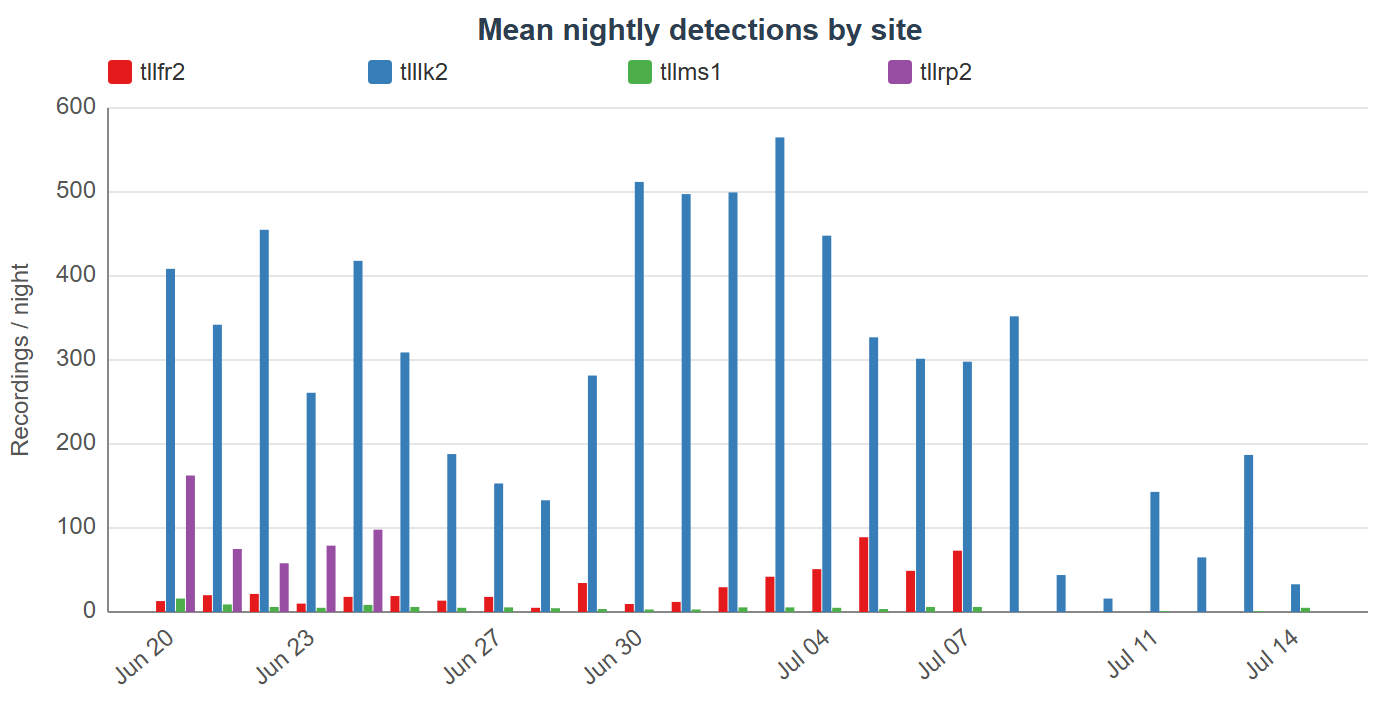
\includegraphics[width=1\linewidth,height=\textheight,keepaspectratio]{Figures/AppendixB/5006_bar.png}

}

\caption{Nightly activity by site (2025 top, 2024 below), cell 5006 -
Petersburg}

\end{figure}%

\newpage

\begin{figure}[H]

{\centering 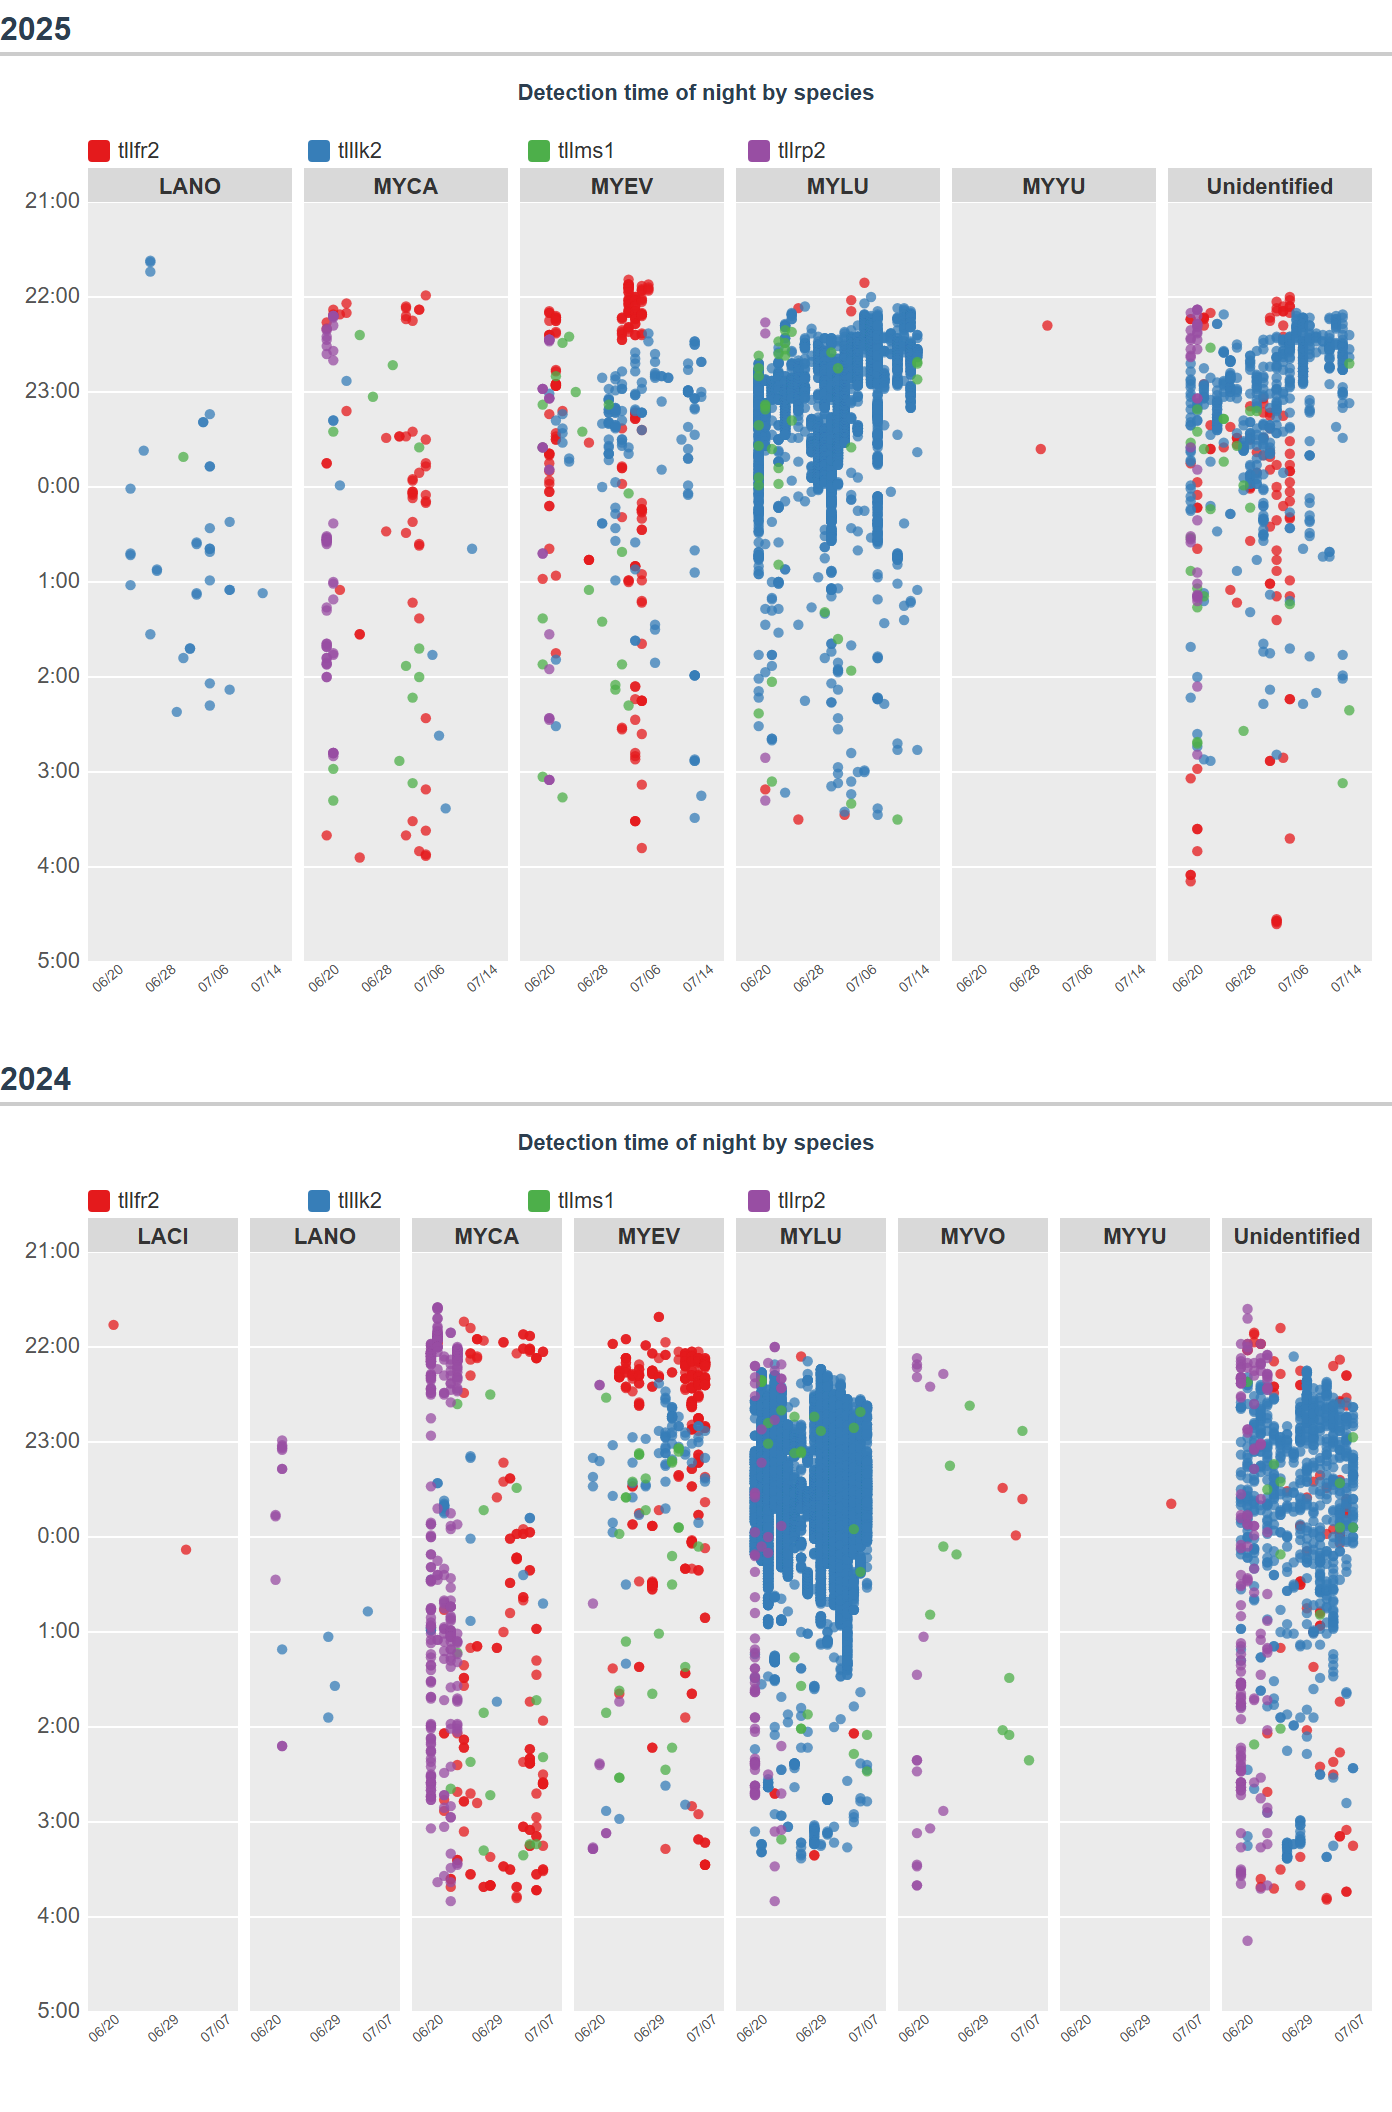
\includegraphics[width=1\linewidth,height=\textheight,keepaspectratio]{Figures/AppendixB/5006_hour.png}

}

\caption{Detection times by species and site (2025 top, 2024 below),
cell 5006 - Petersburg}

\end{figure}%

\newpage

\subsection*{Grid cell 18318 -
Wrangell}\label{grid-cell-18318---wrangell}

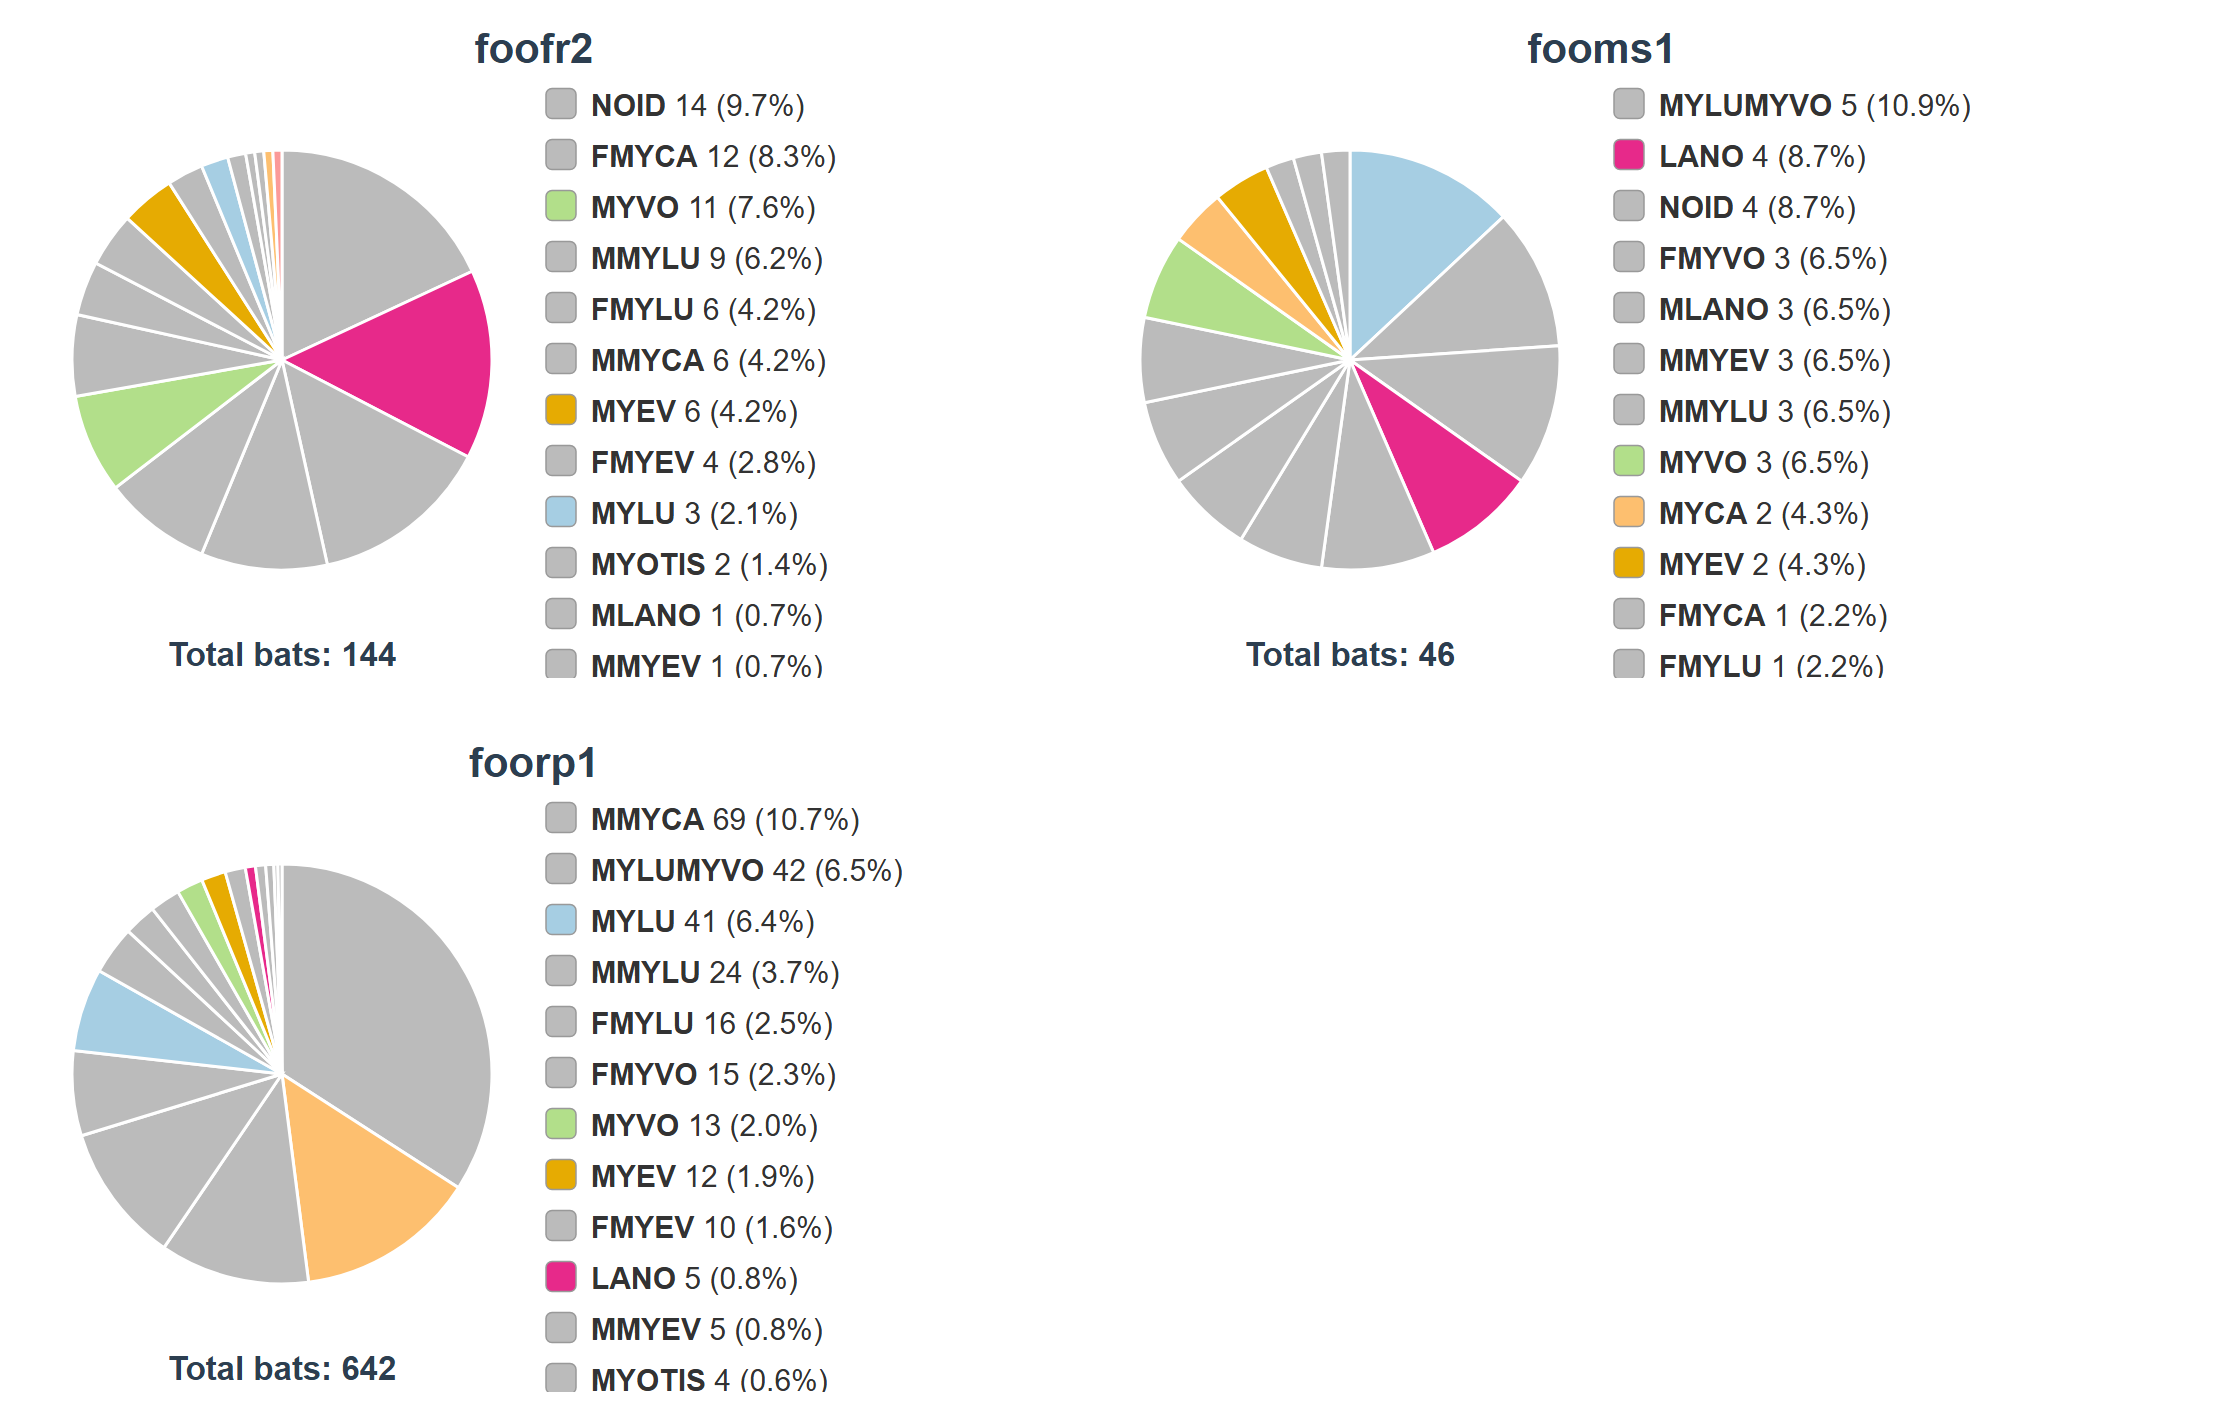
\includegraphics[width=1\linewidth,height=\textheight,keepaspectratio]{Figures/AppendixB/18318_pies.png}

\newpage

\begin{figure}[H]

{\centering 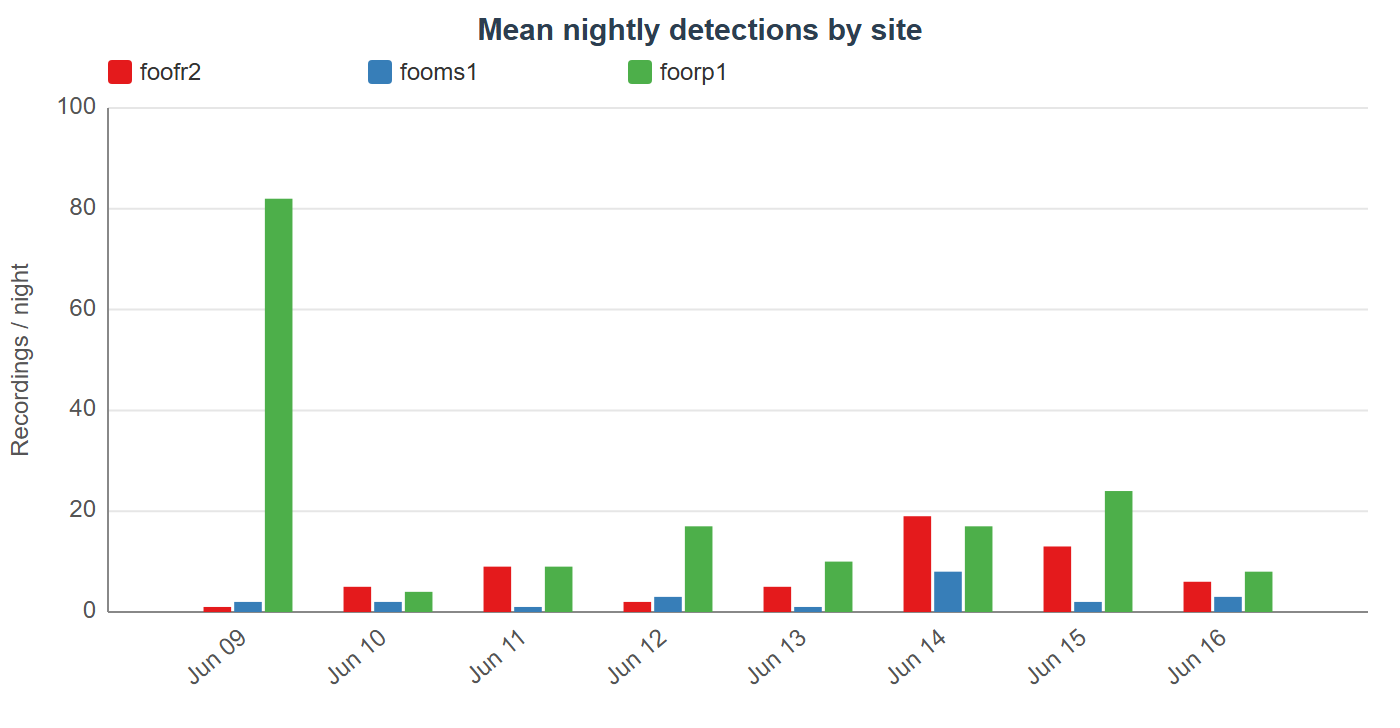
\includegraphics[width=1\linewidth,height=\textheight,keepaspectratio]{Figures/AppendixB/18318_bar.png}

}

\caption{Nightly activity by site (2025 top, 2024 below), cell 18318 -
Wrangell}

\end{figure}%

\newpage

\begin{figure}[H]

{\centering 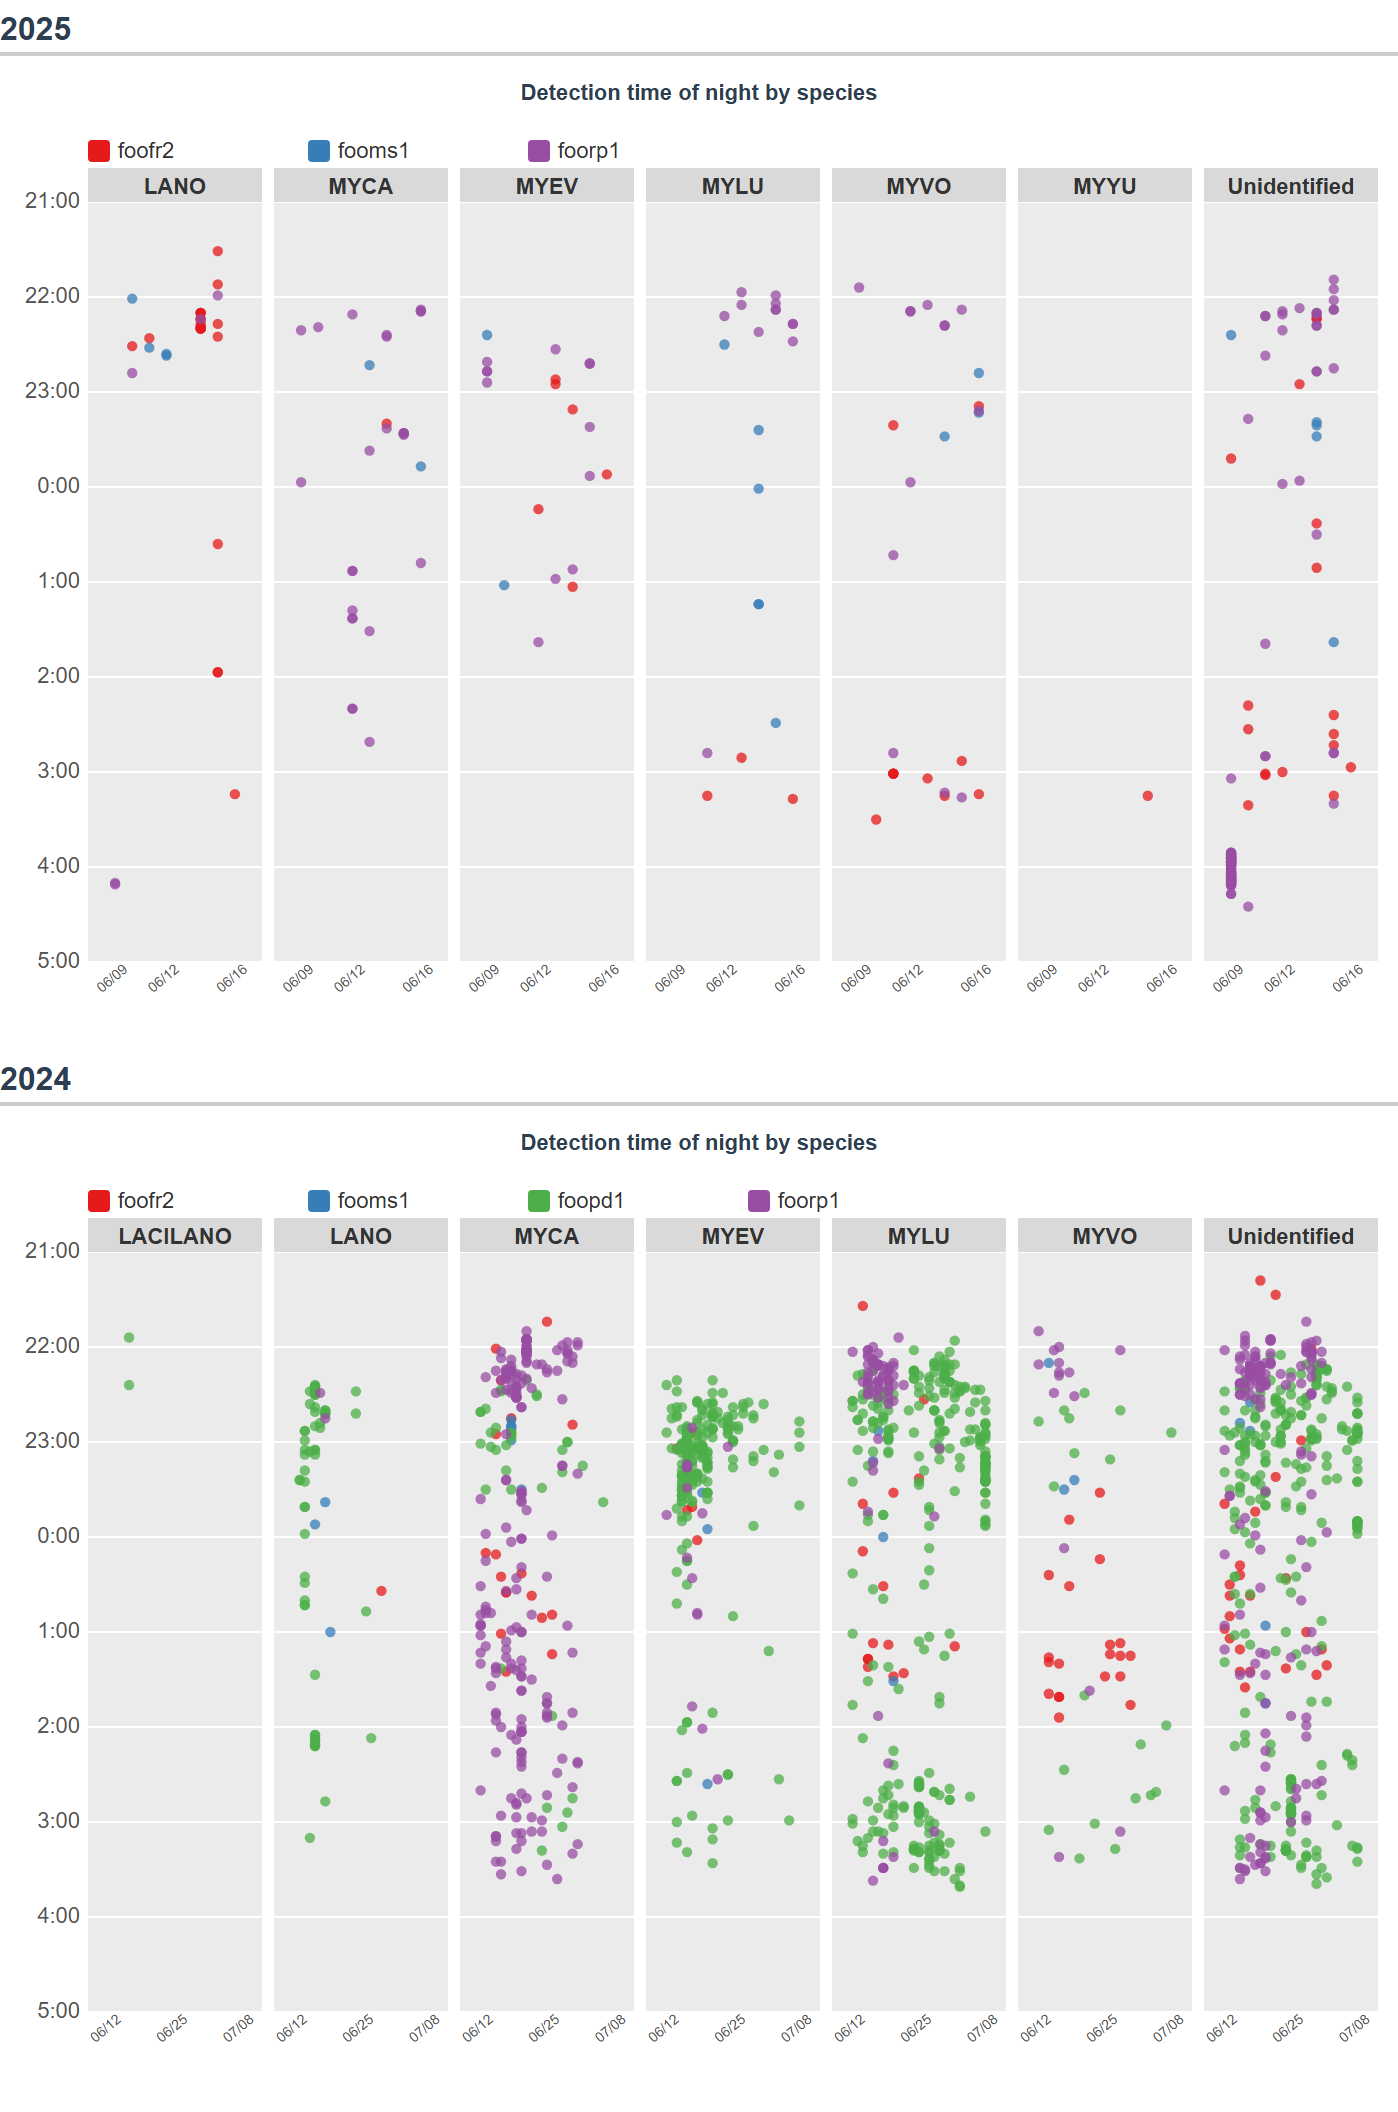
\includegraphics[width=1\linewidth,height=\textheight,keepaspectratio]{Figures/AppendixB/18318_hour.png}

}

\caption{Detection times by species and site (2025 top, 2024 below),
cell 18318 - Wrangell}

\end{figure}%

\newpage

\subsection*{Grid cell 31438 - Douglas}\label{grid-cell-31438---douglas}

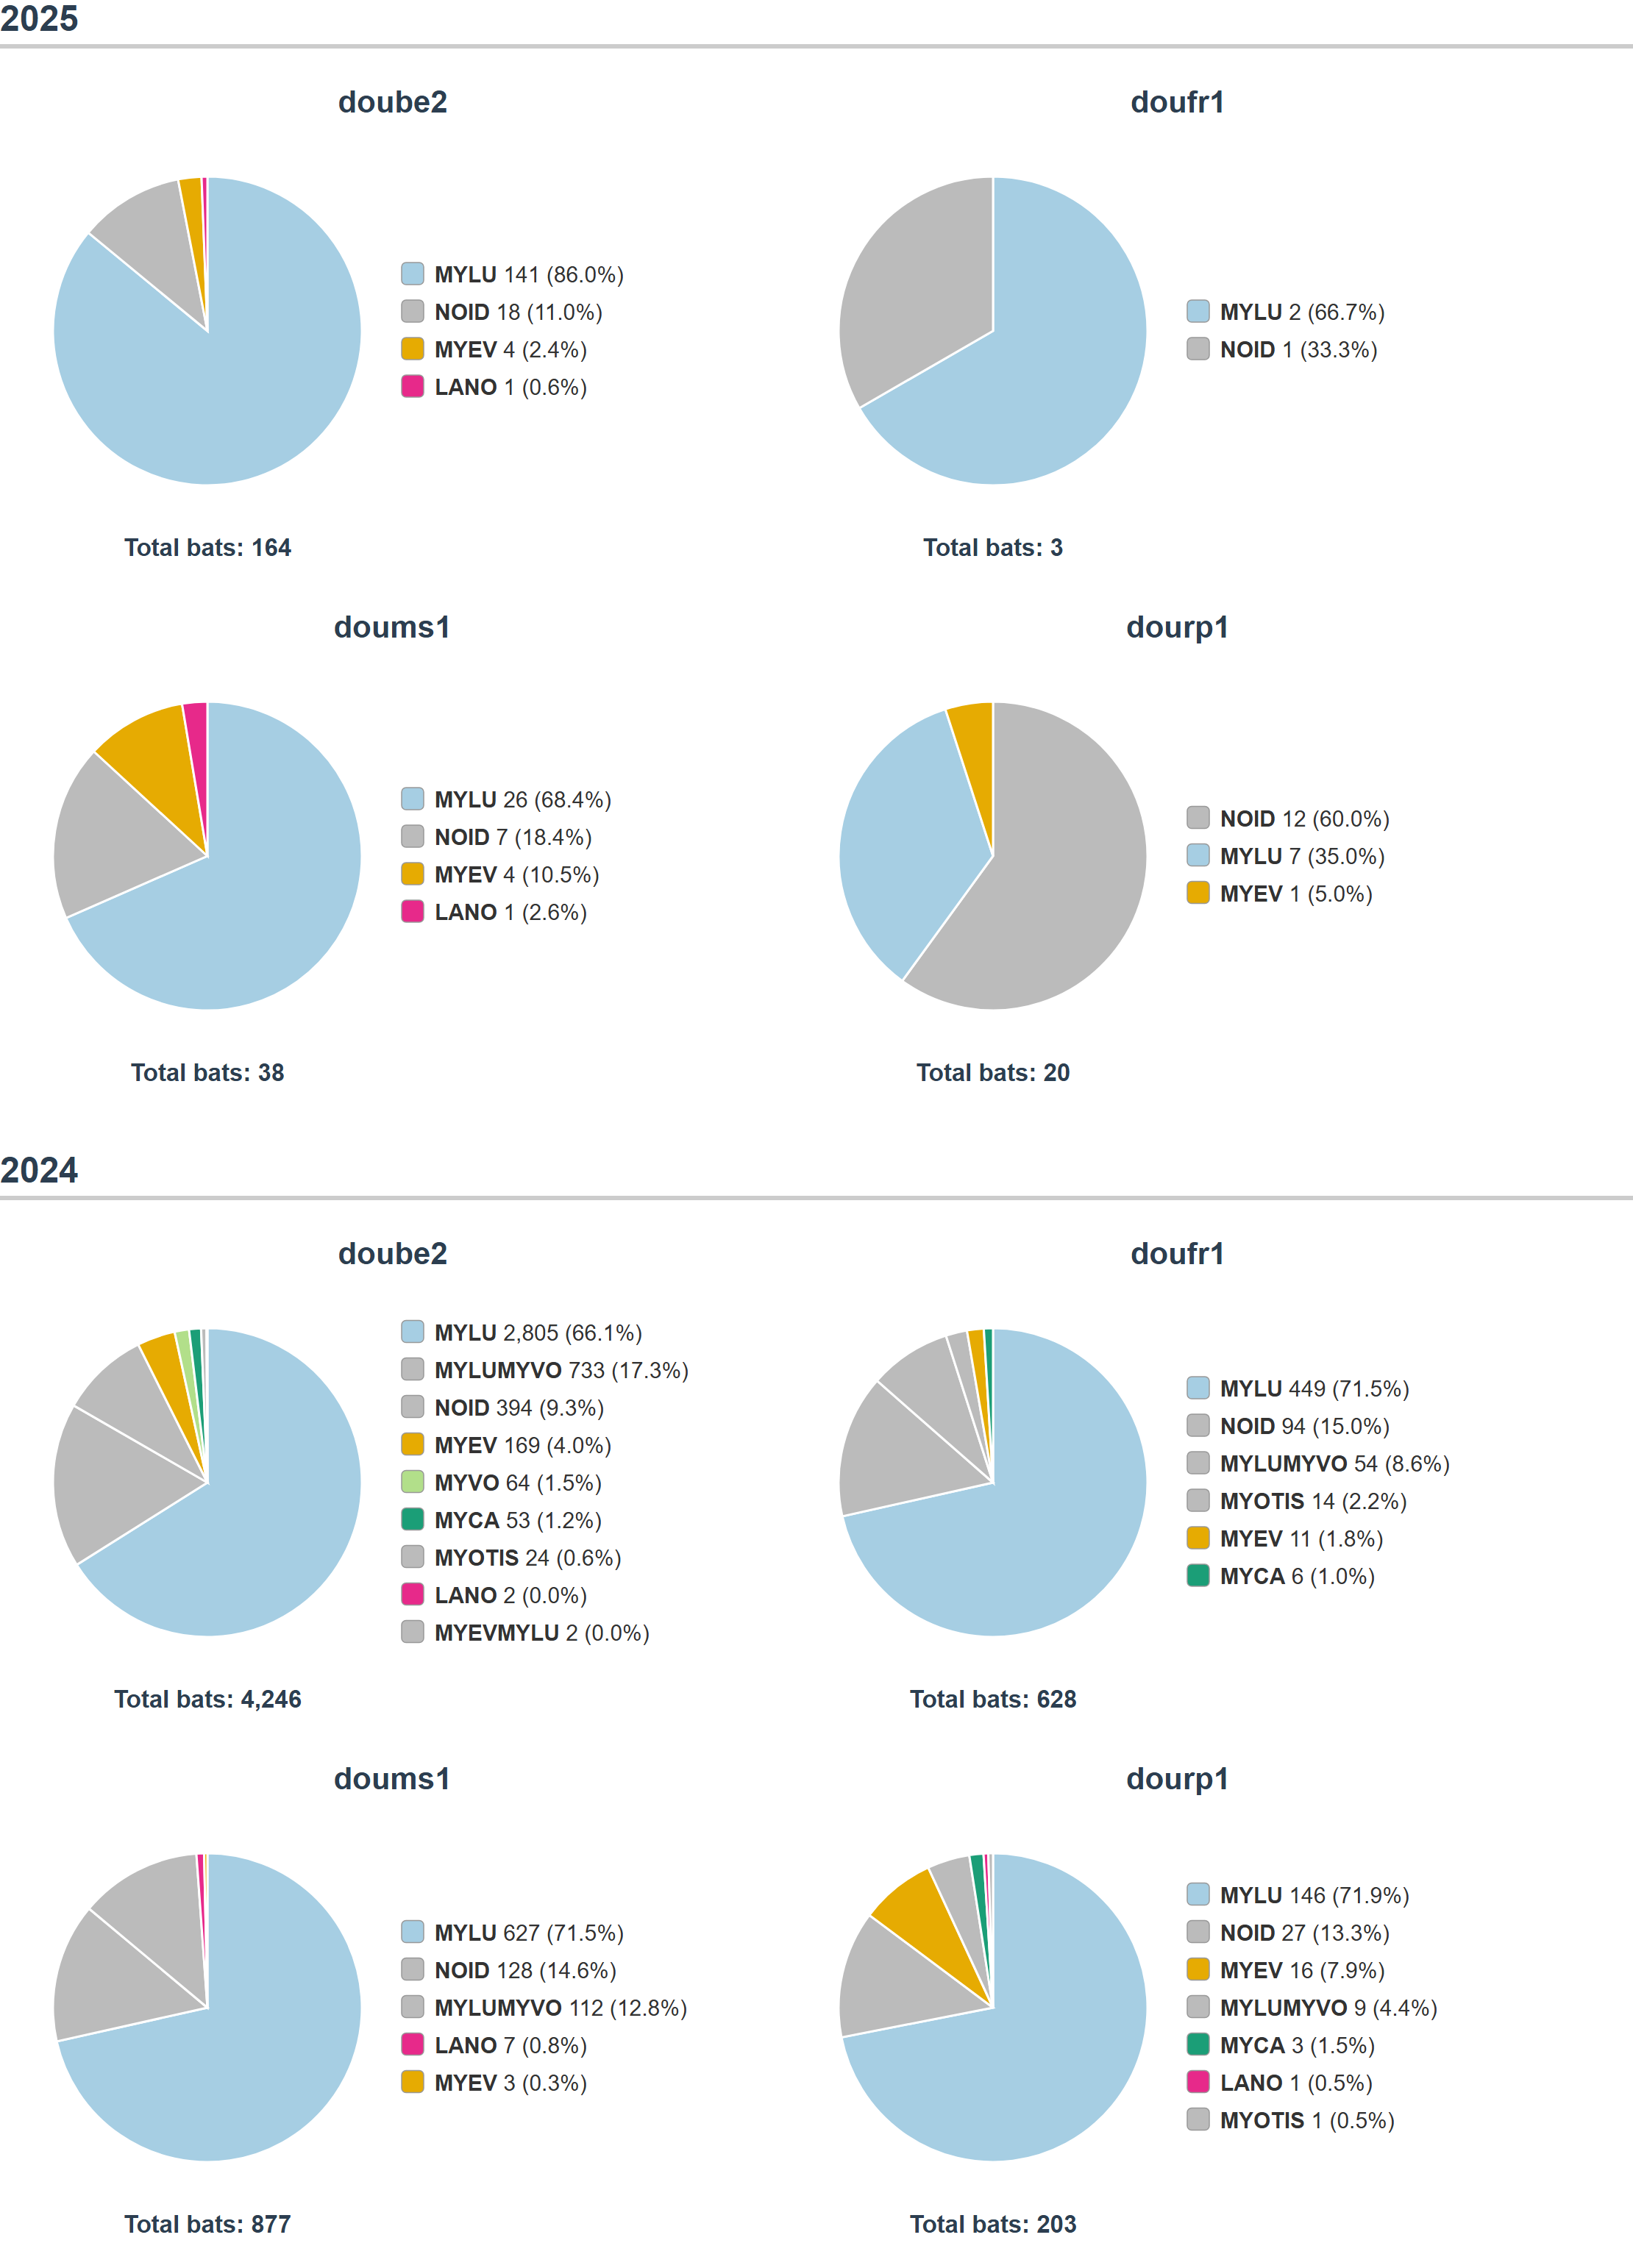
\includegraphics[width=1\linewidth,height=\textheight,keepaspectratio]{Figures/AppendixB/31438_pies.png}

\newpage

\begin{figure}[H]

{\centering 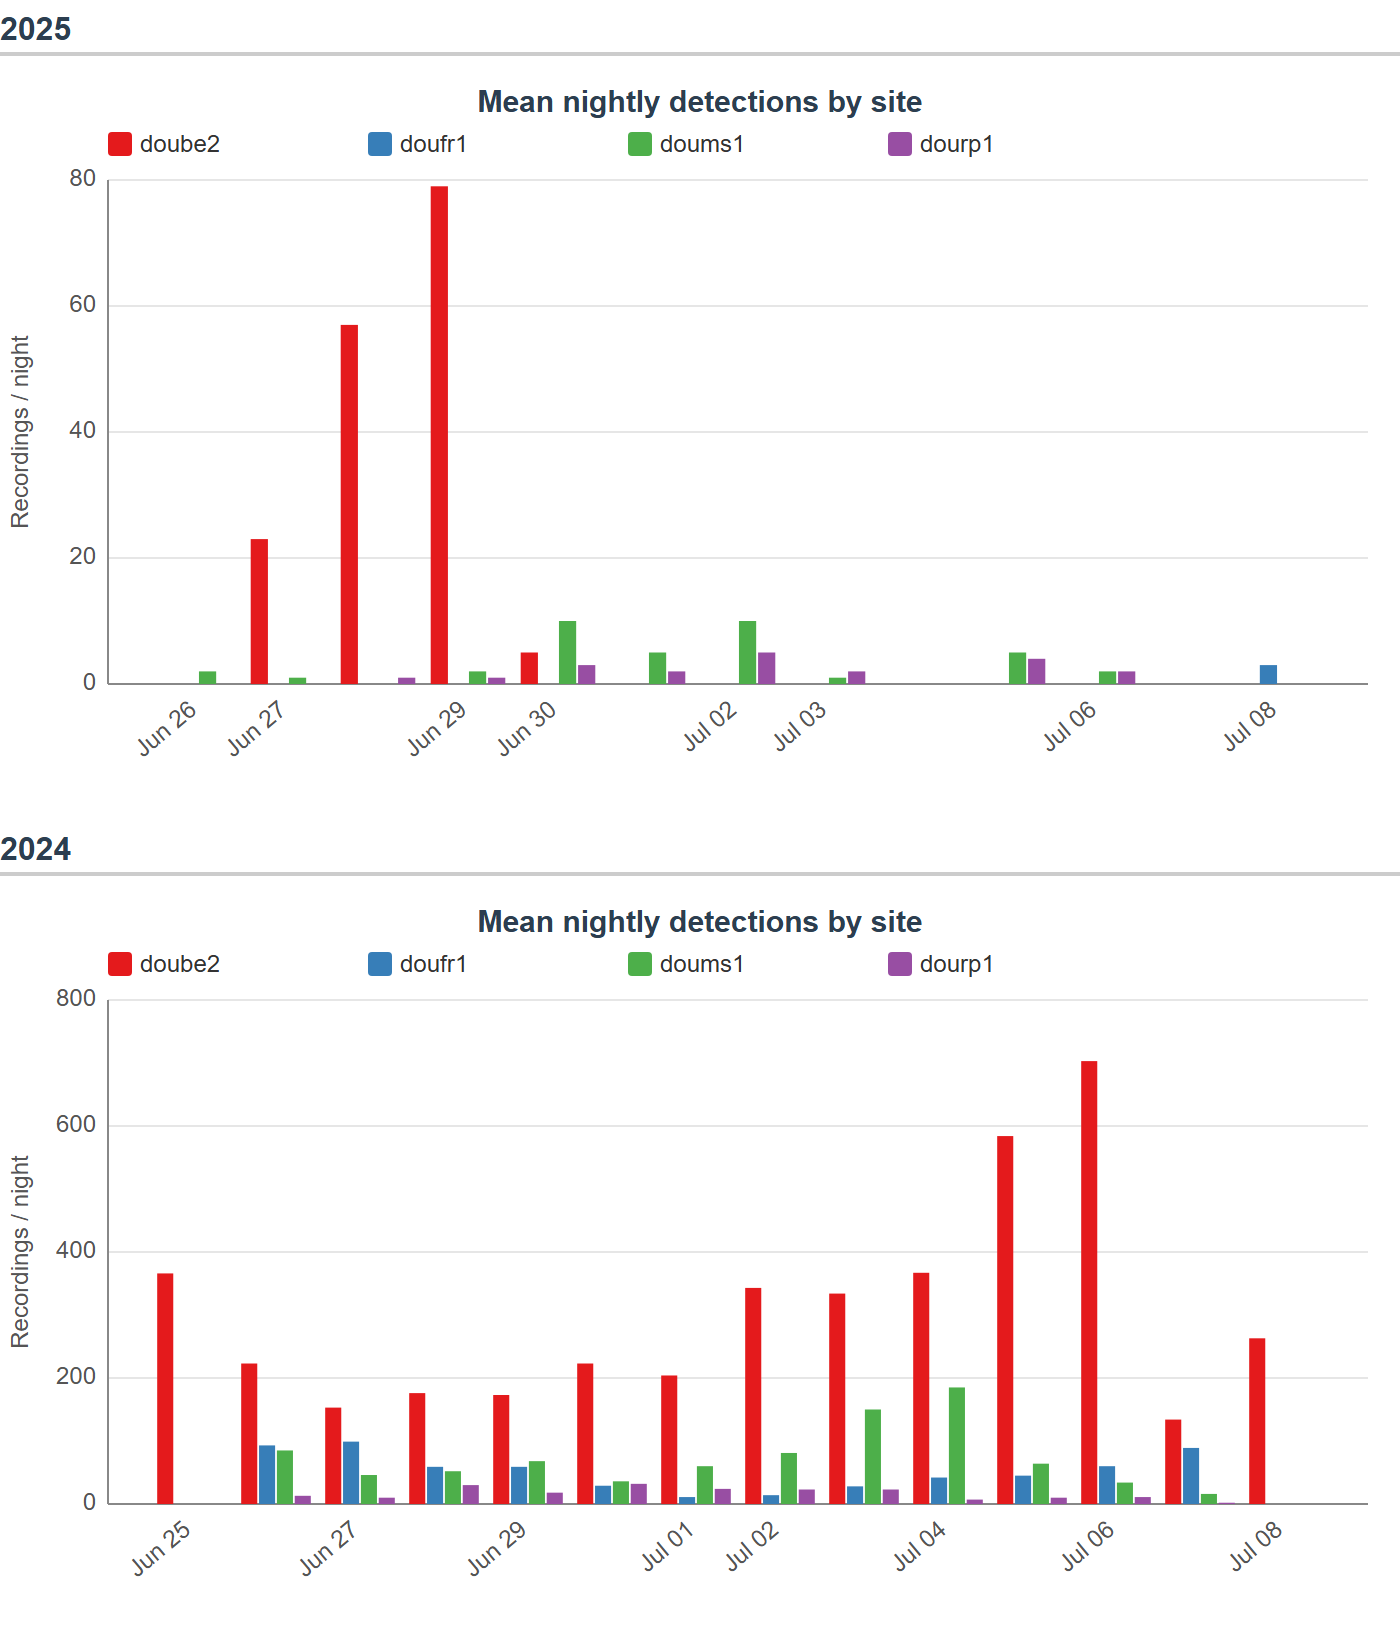
\includegraphics[width=1\linewidth,height=\textheight,keepaspectratio]{Figures/AppendixB/31438_bar.png}

}

\caption{Nightly activity by site (2025 top, 2024 below), cell 31438 -
Douglas}

\end{figure}%

\newpage

\begin{figure}[H]

{\centering 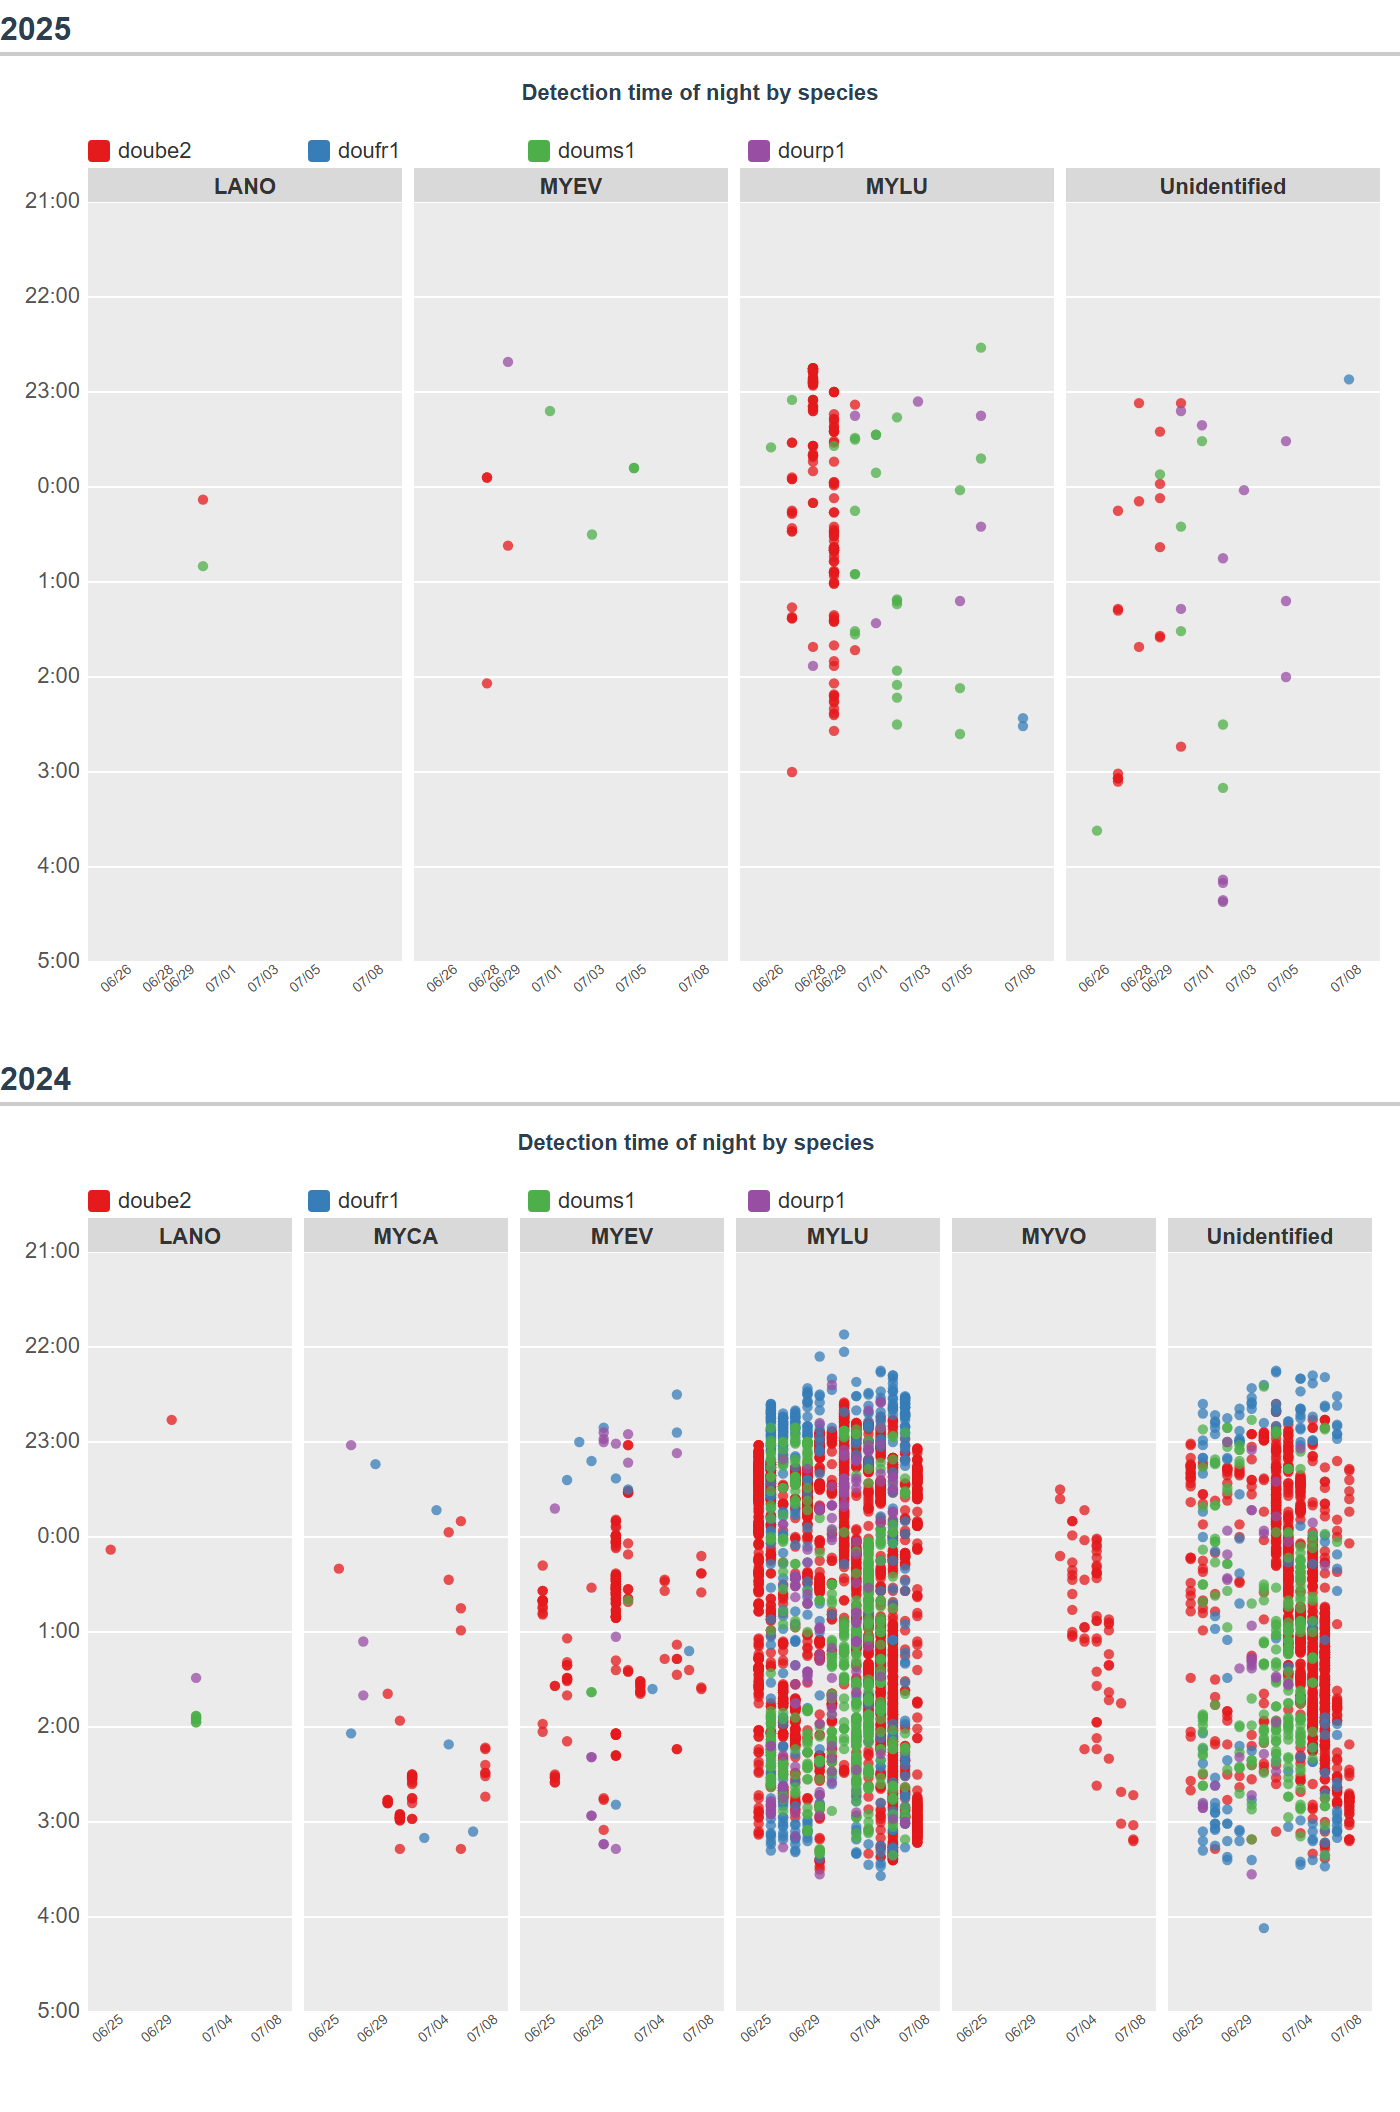
\includegraphics[width=1\linewidth,height=\textheight,keepaspectratio]{Figures/AppendixB/31438_hour.png}

}

\caption{Detection times by species and site (2025 top, 2024 below),
cell 31438 - Douglas}

\end{figure}%

\newpage

\subsection*{Grid cell 33486 - Sitka}\label{grid-cell-33486---sitka}

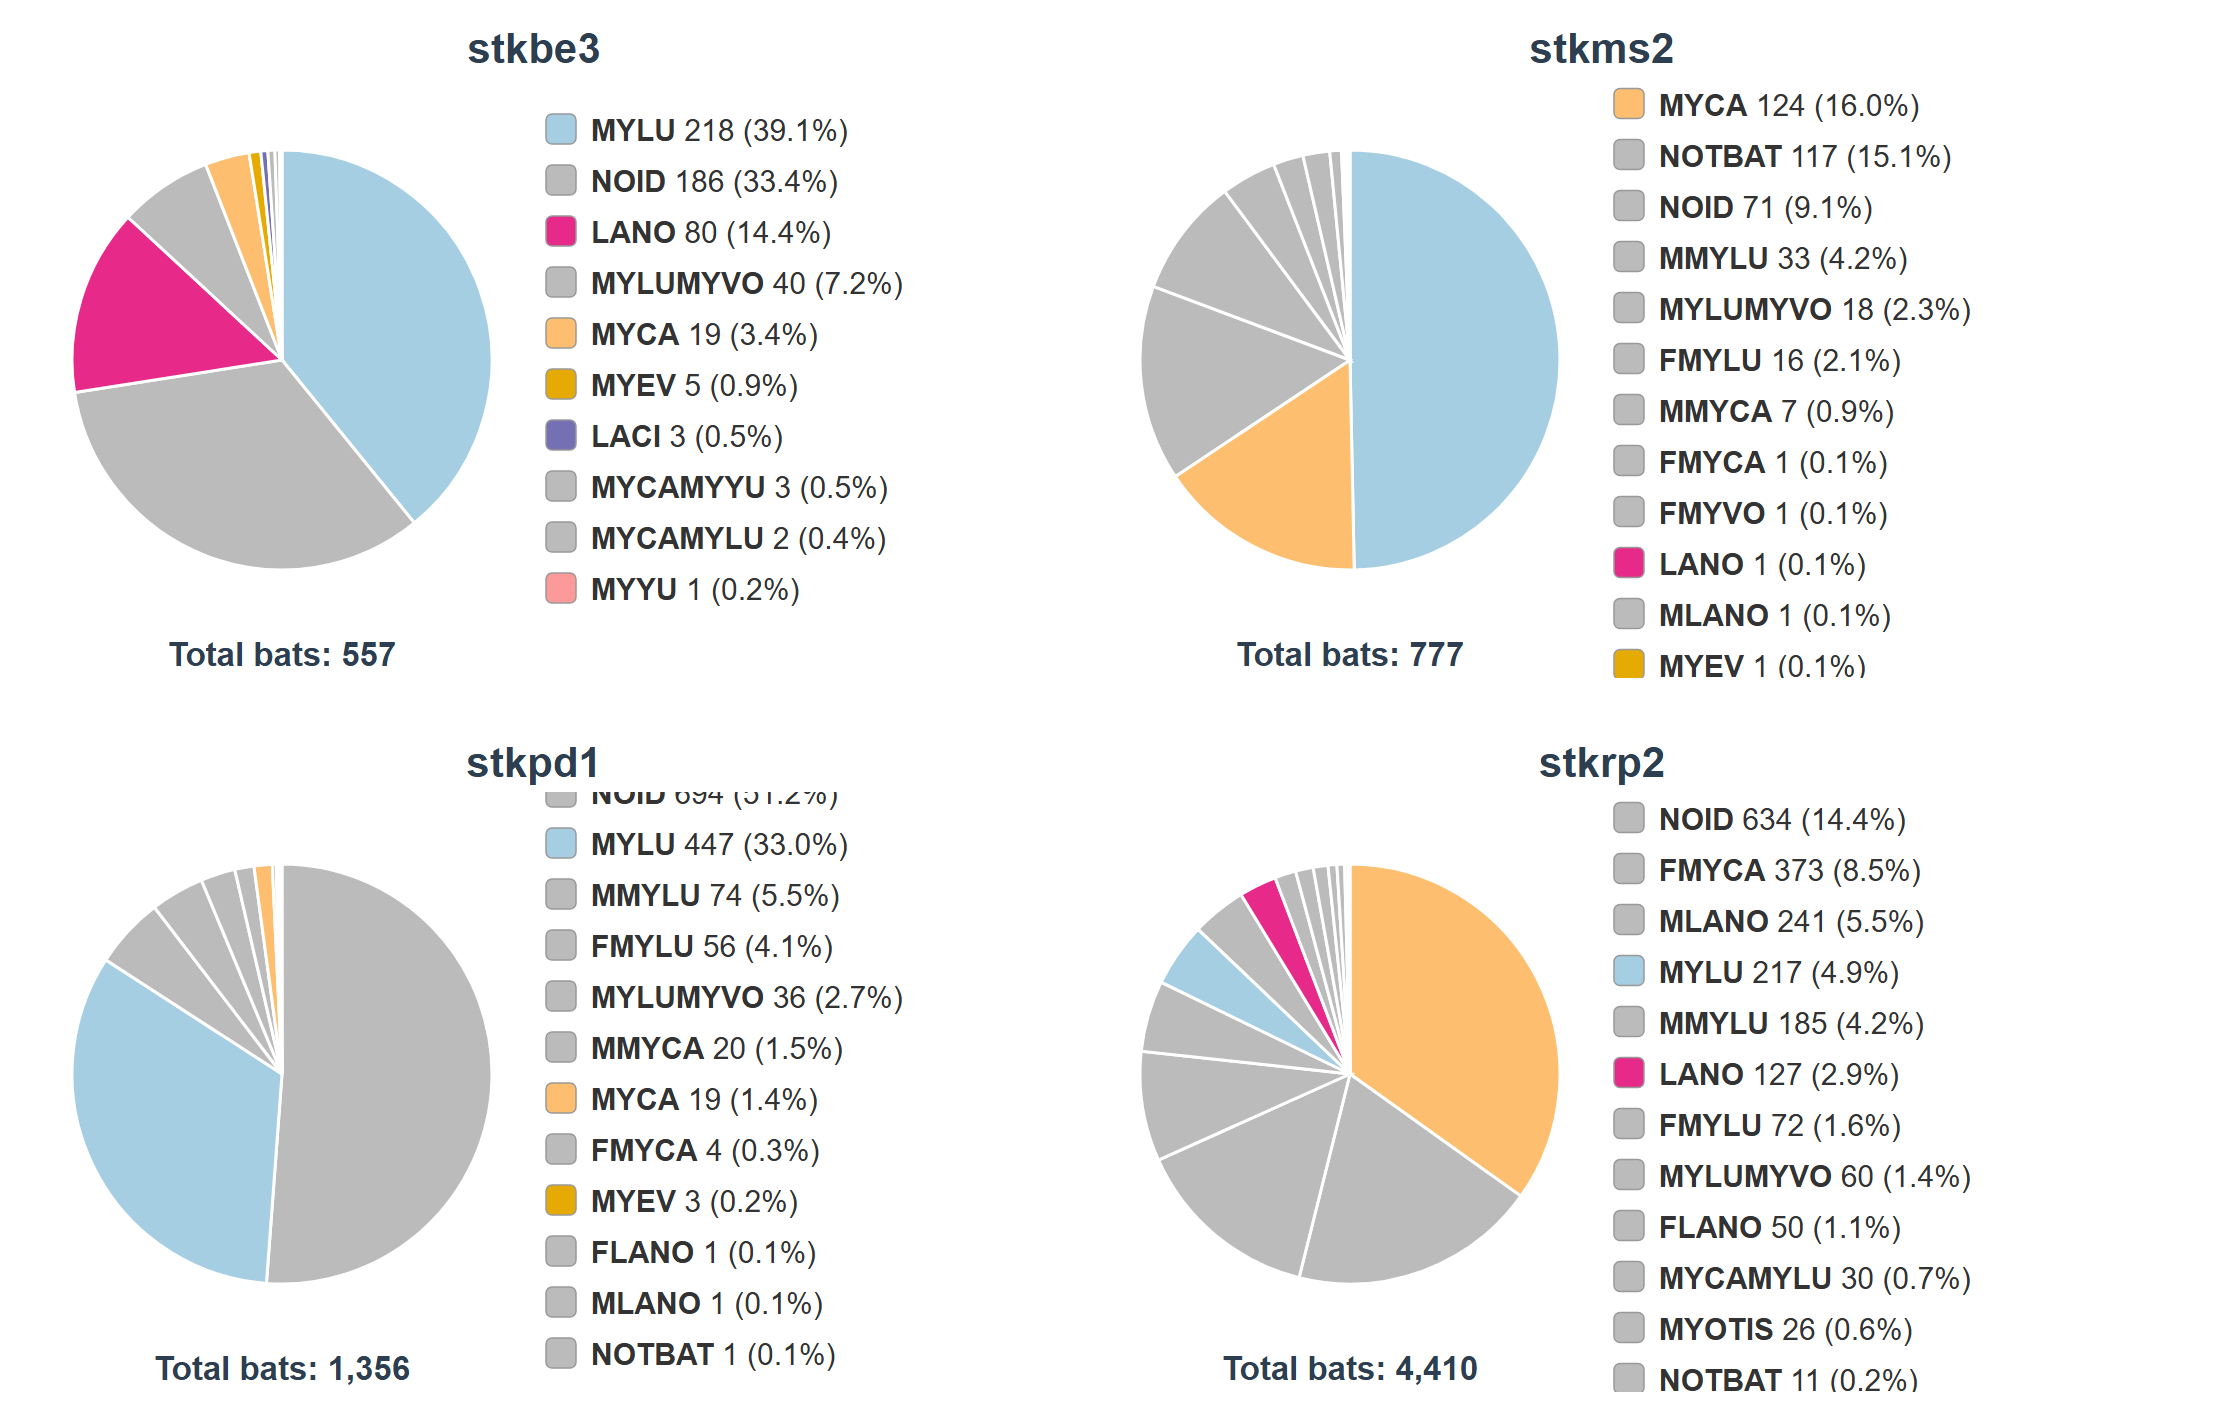
\includegraphics[width=1\linewidth,height=\textheight,keepaspectratio]{Figures/AppendixB/33486_pies.png}

\newpage

\begin{figure}[H]

{\centering 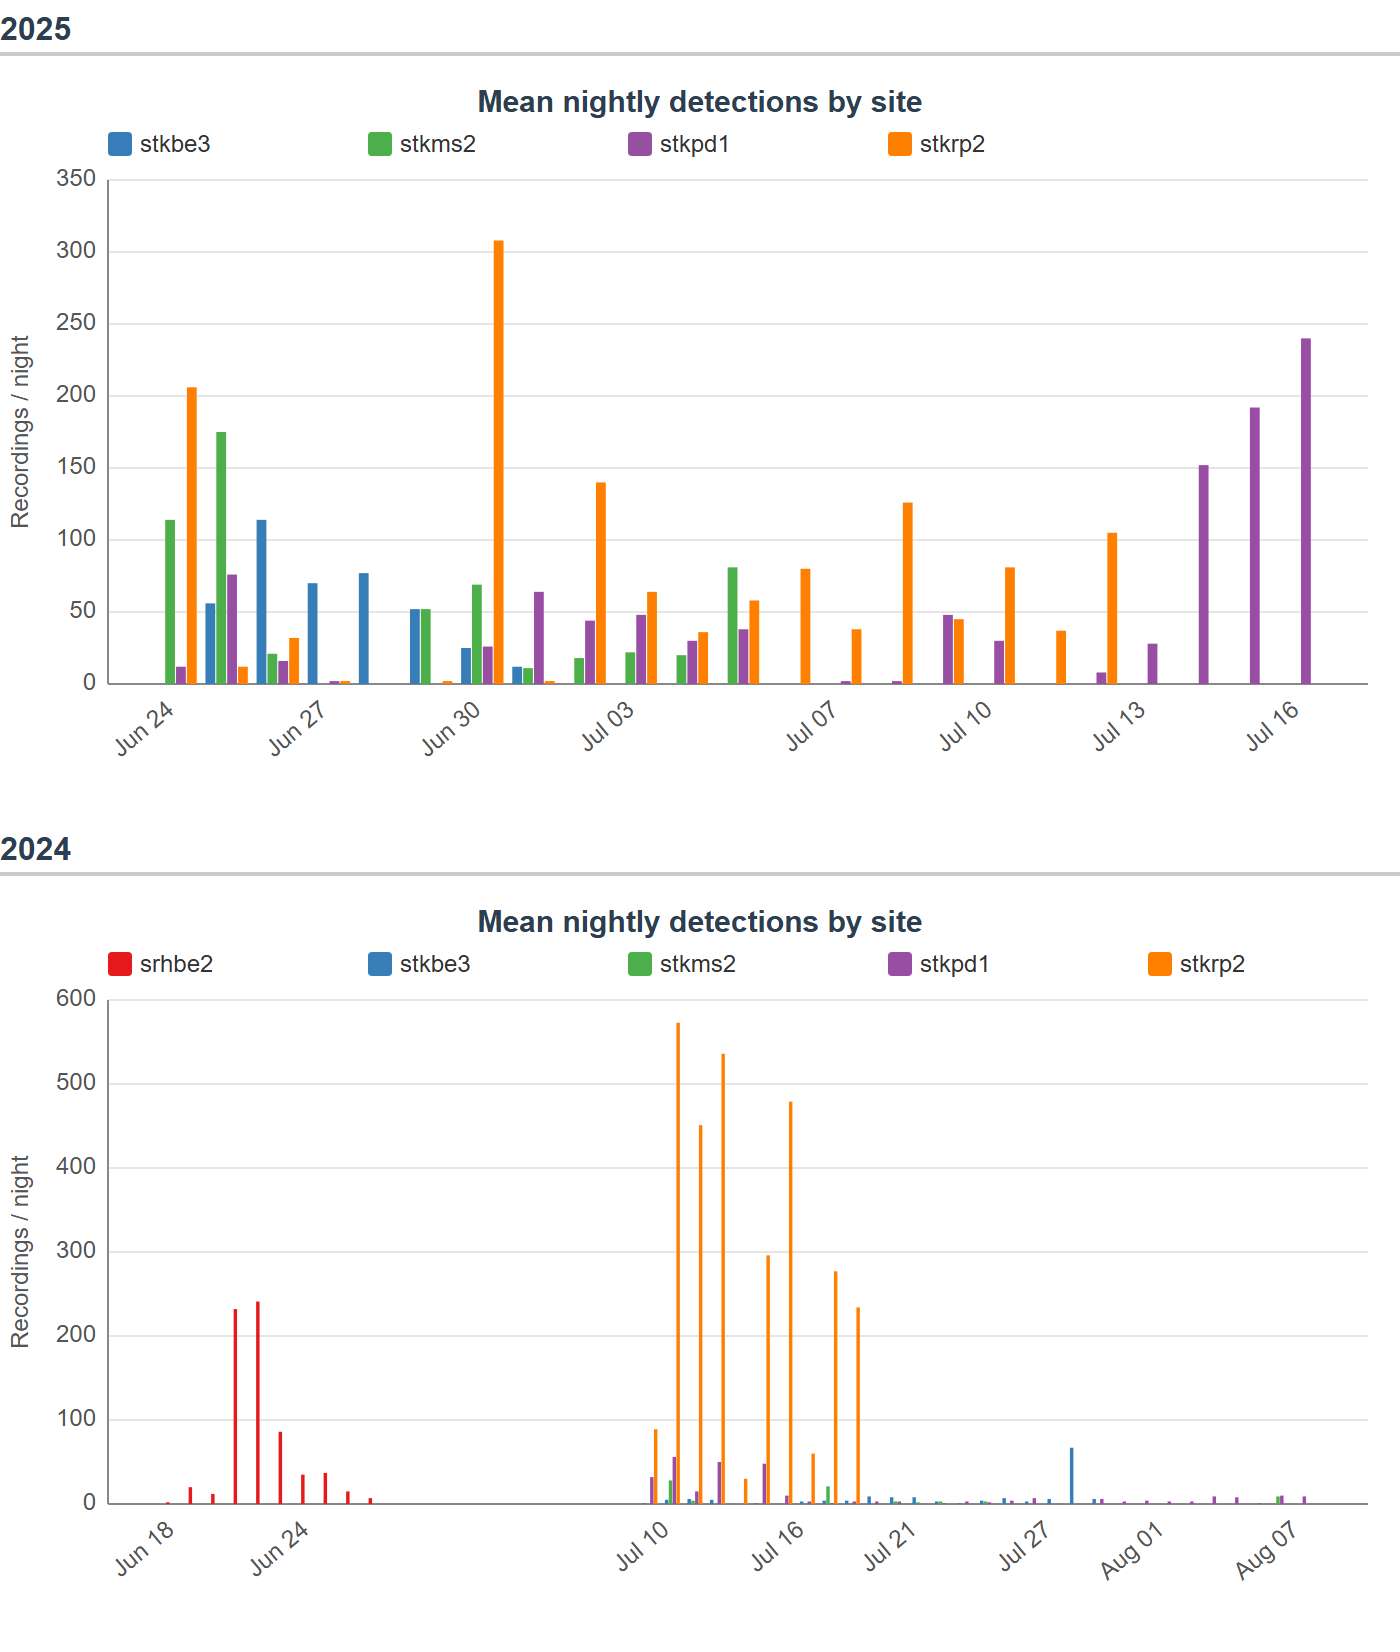
\includegraphics[width=1\linewidth,height=\textheight,keepaspectratio]{Figures/AppendixB/33486_bar.png}

}

\caption{Nightly activity by site (2025 top, 2024 below), cell 33486 -
Sitka}

\end{figure}%

\newpage

\begin{figure}[H]

{\centering 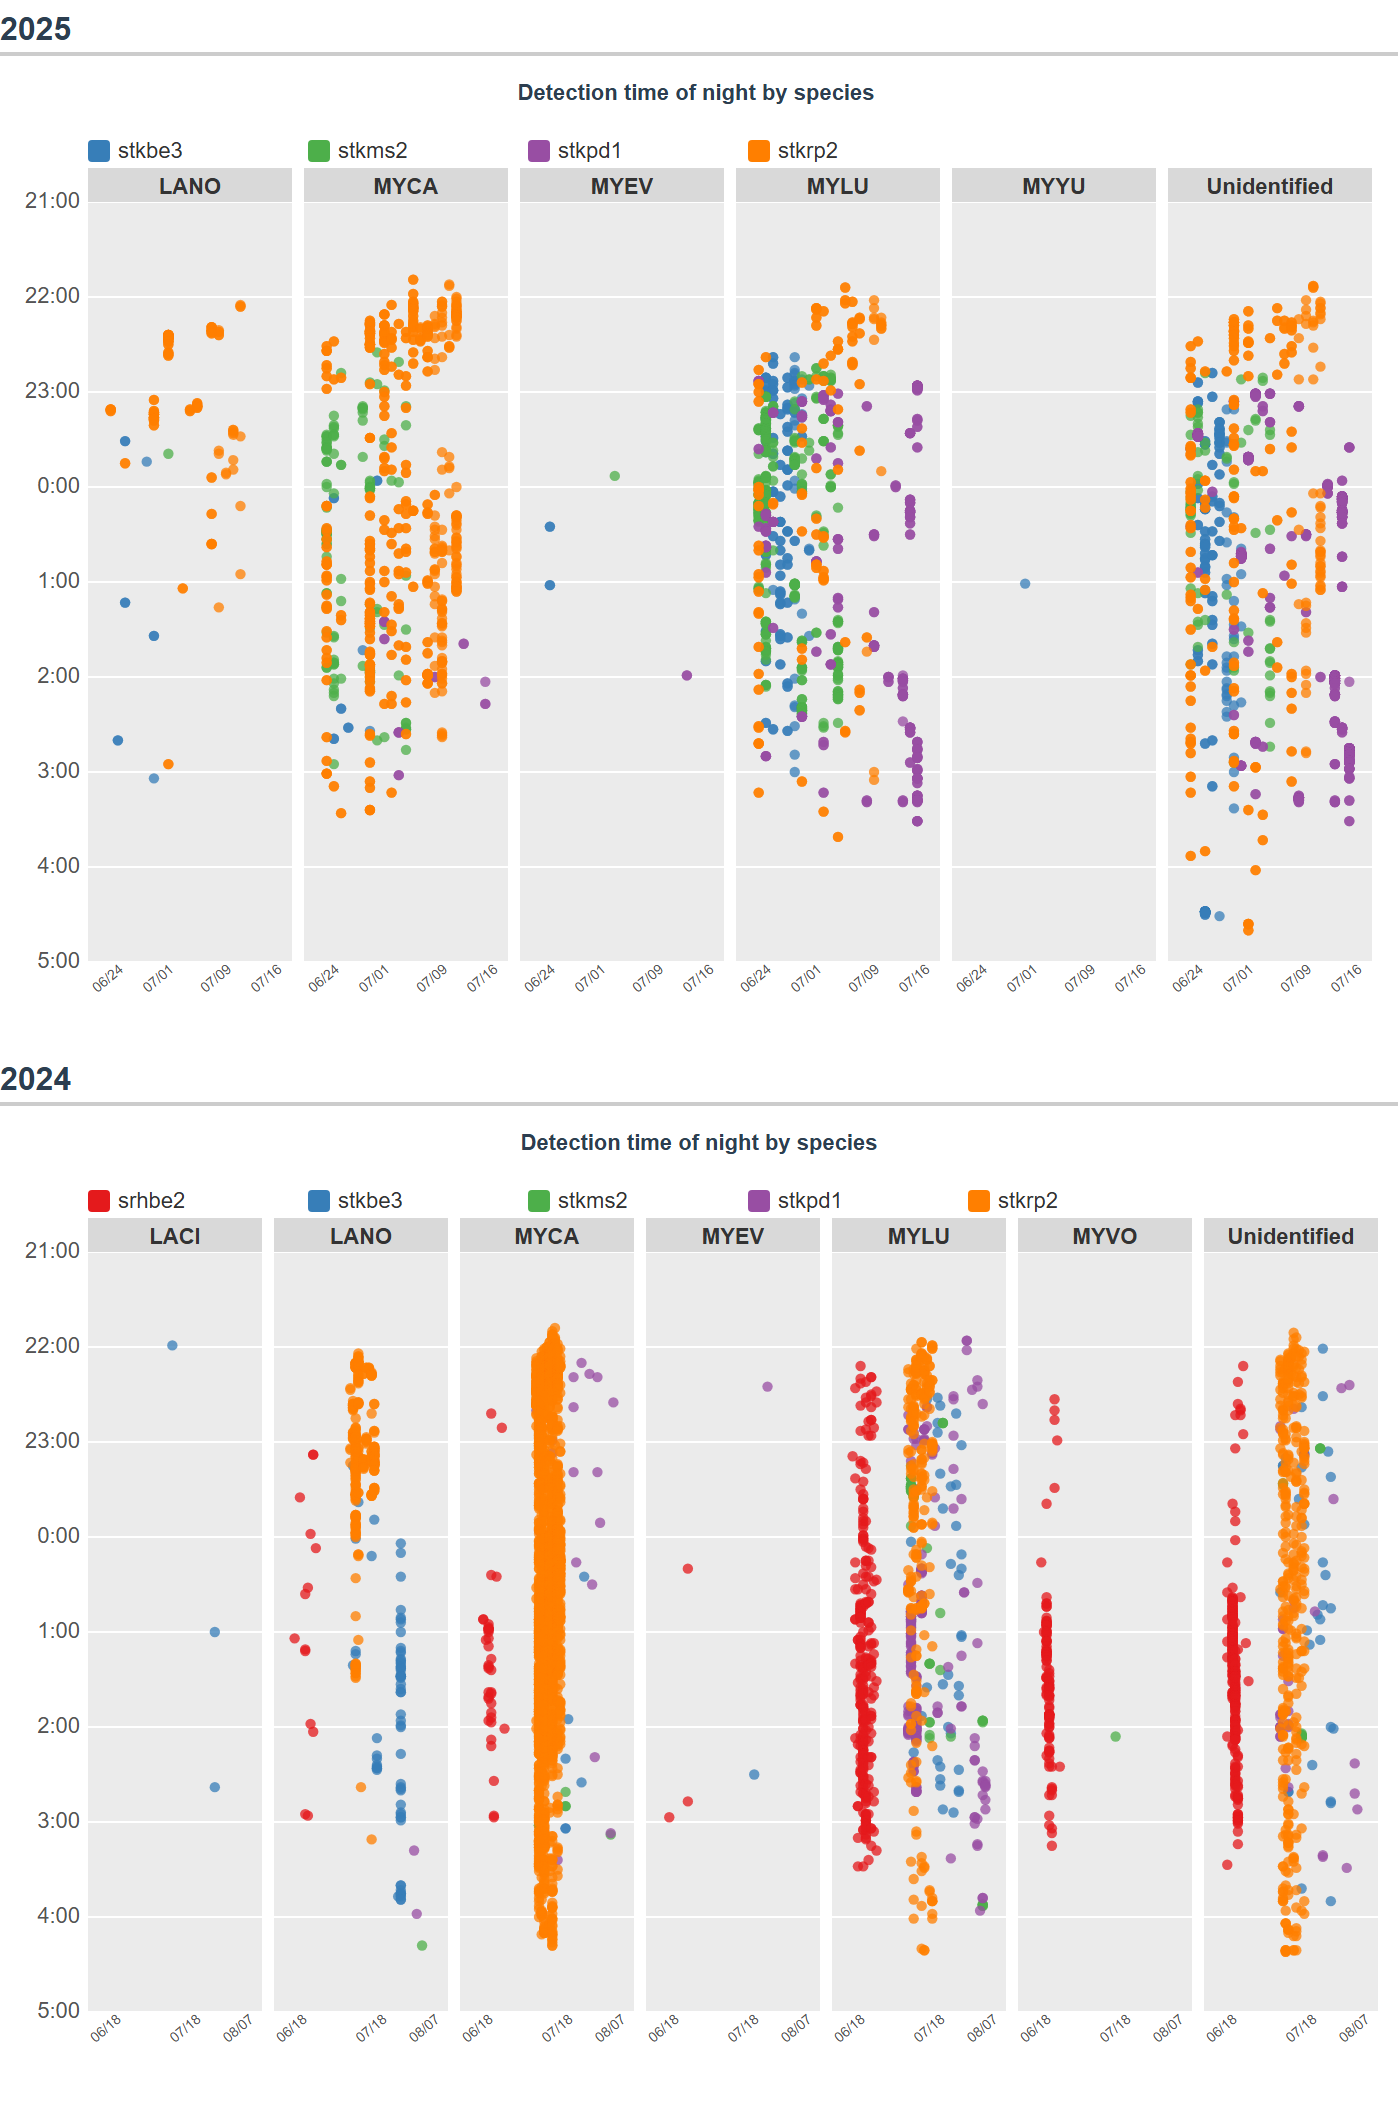
\includegraphics[width=1\linewidth,height=\textheight,keepaspectratio]{Figures/AppendixB/33486_hour.png}

}

\caption{Detection times by species and site (2025 top, 2024 below),
cell 33486 - Sitka}

\end{figure}%

\newpage

\subsection*{Grid cell 34254 - Hoonah}\label{grid-cell-34254---hoonah}

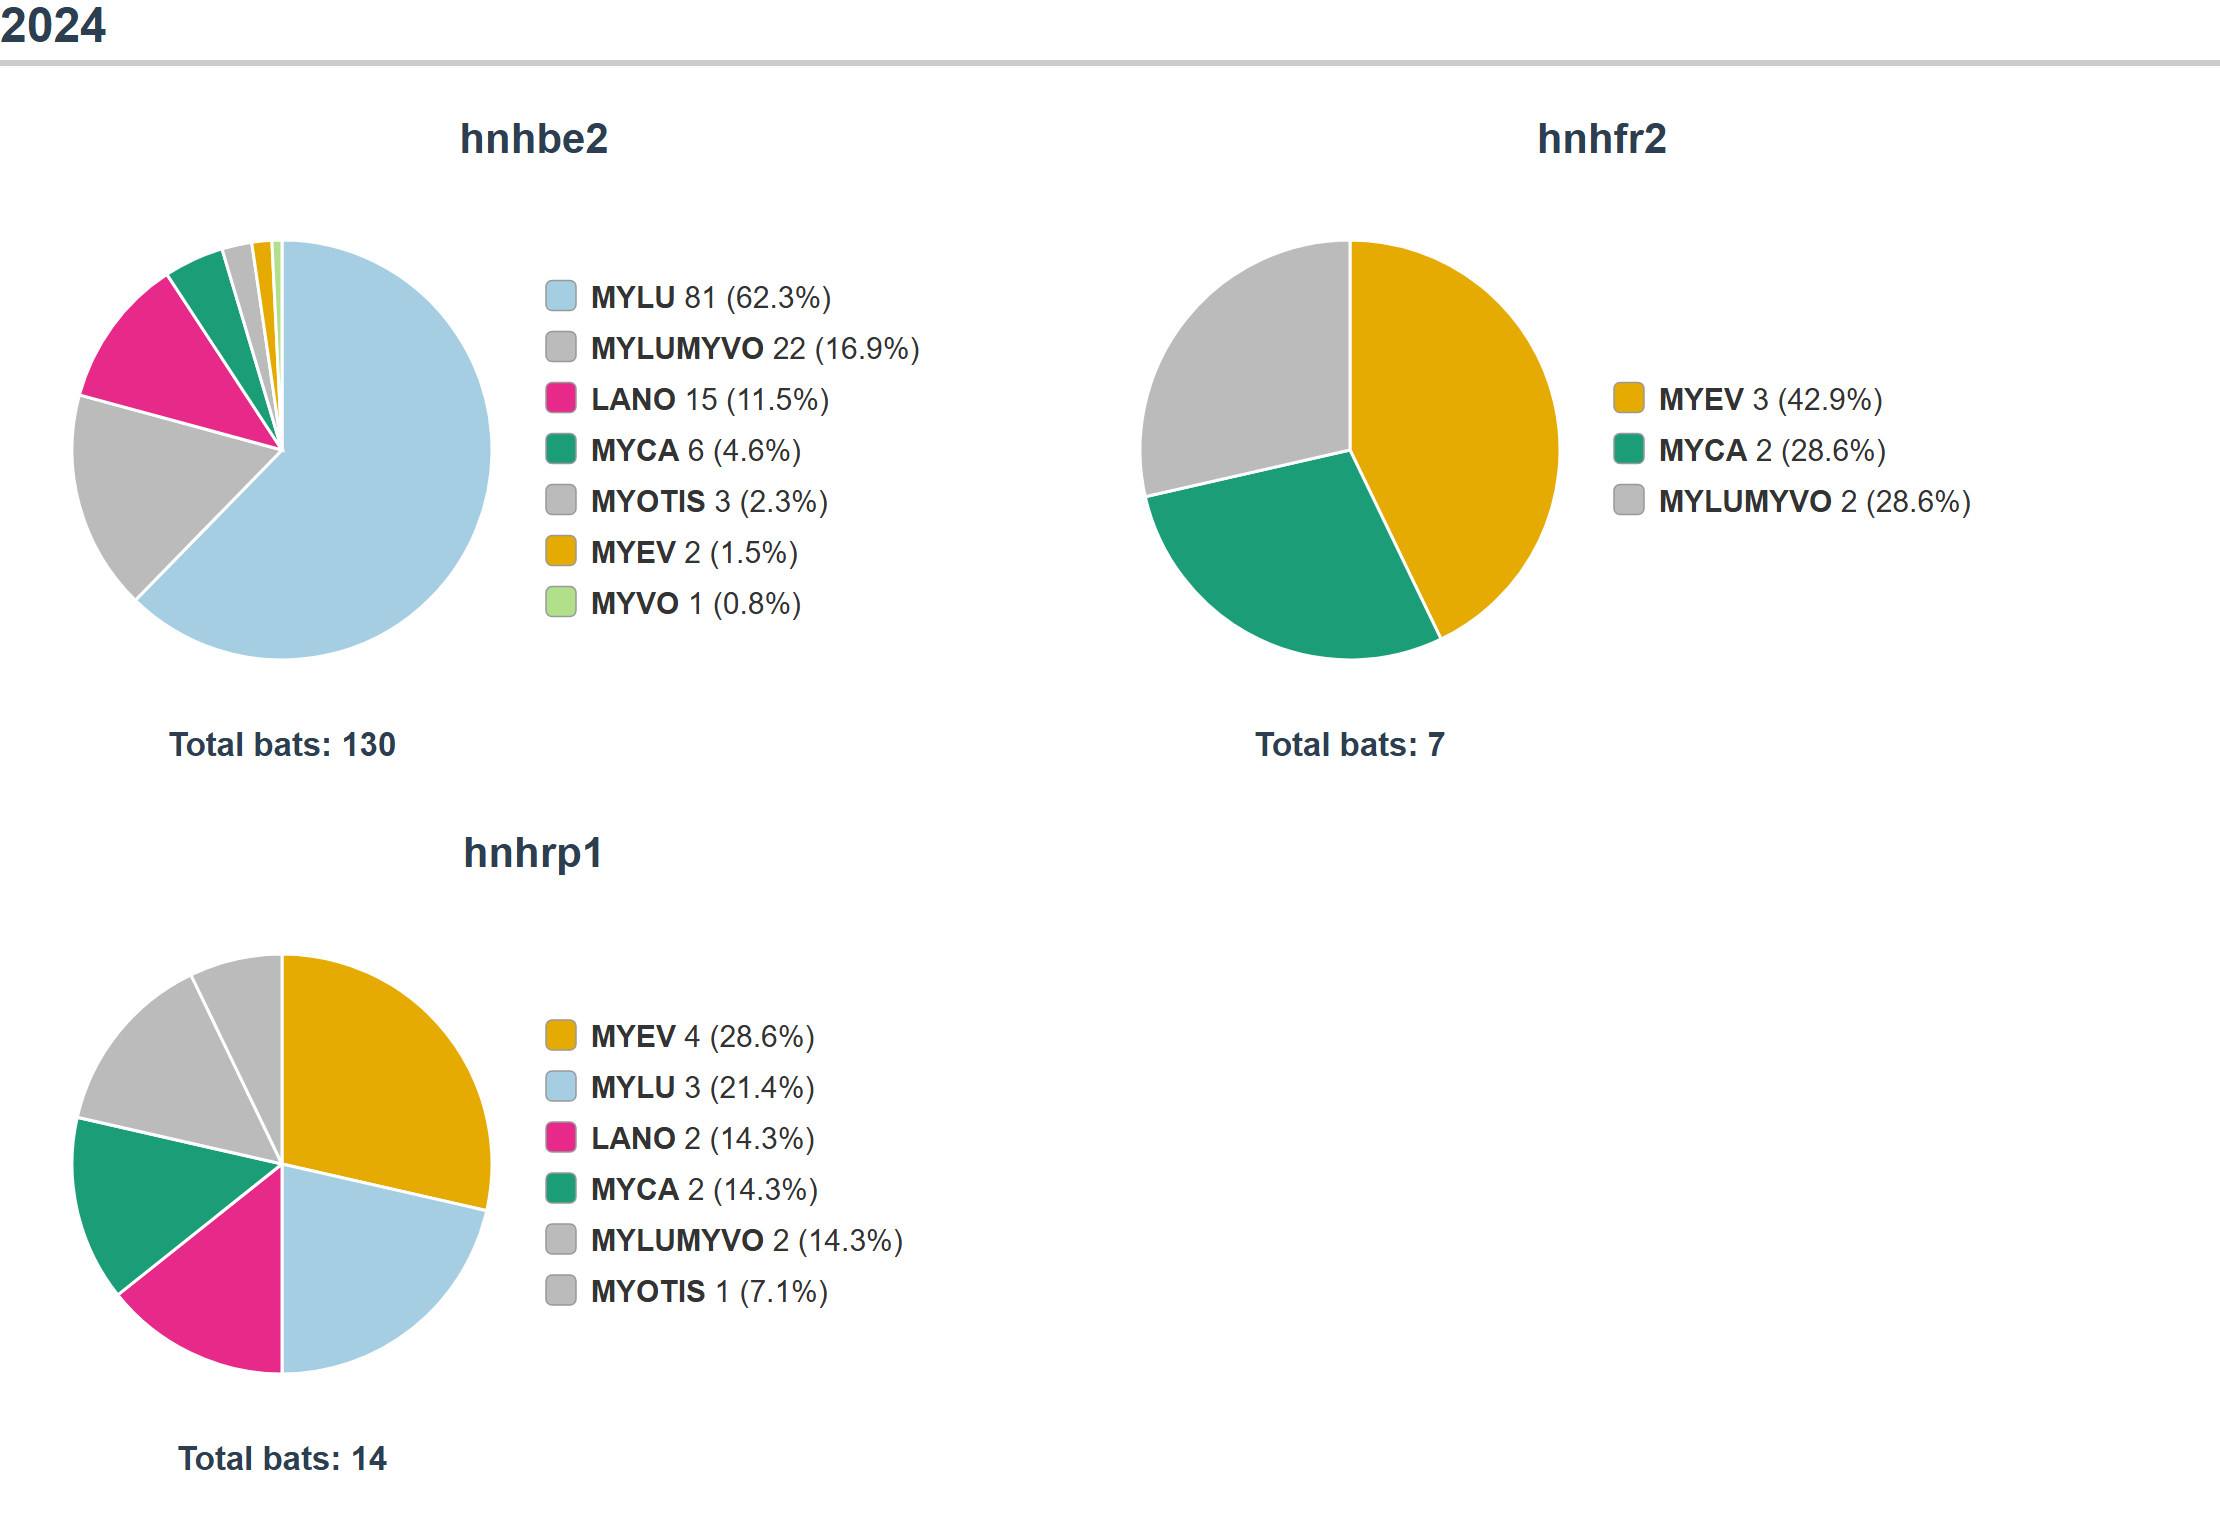
\includegraphics[width=1\linewidth,height=\textheight,keepaspectratio]{Figures/AppendixB/34254_pies.png}

\newpage

\begin{figure}[H]

{\centering 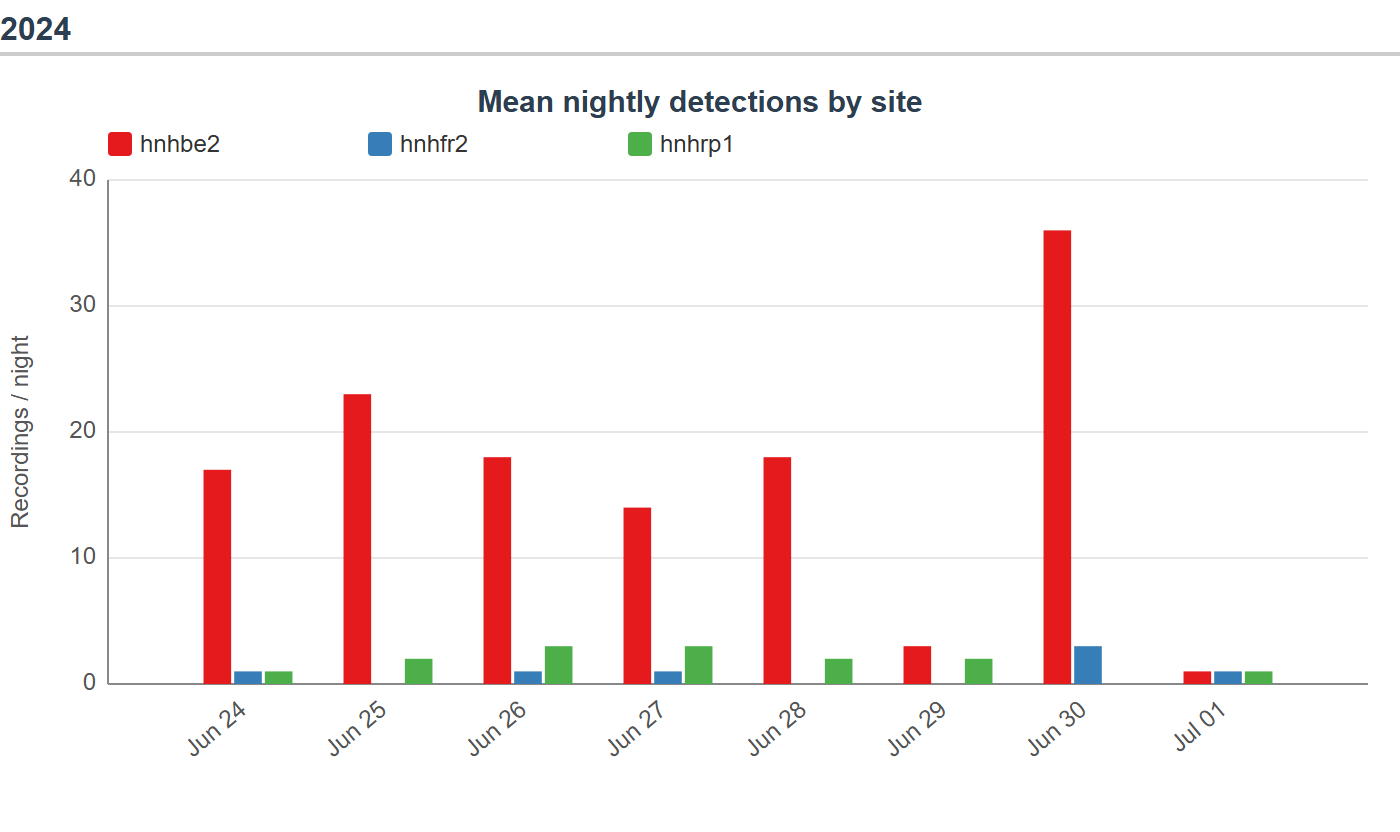
\includegraphics[width=1\linewidth,height=\textheight,keepaspectratio]{Figures/AppendixB/34254_bar.png}

}

\caption{Nightly activity by site (2025 top, 2024 below), cell 34254 -
Hoonah}

\end{figure}%

\newpage

\begin{figure}[H]

{\centering 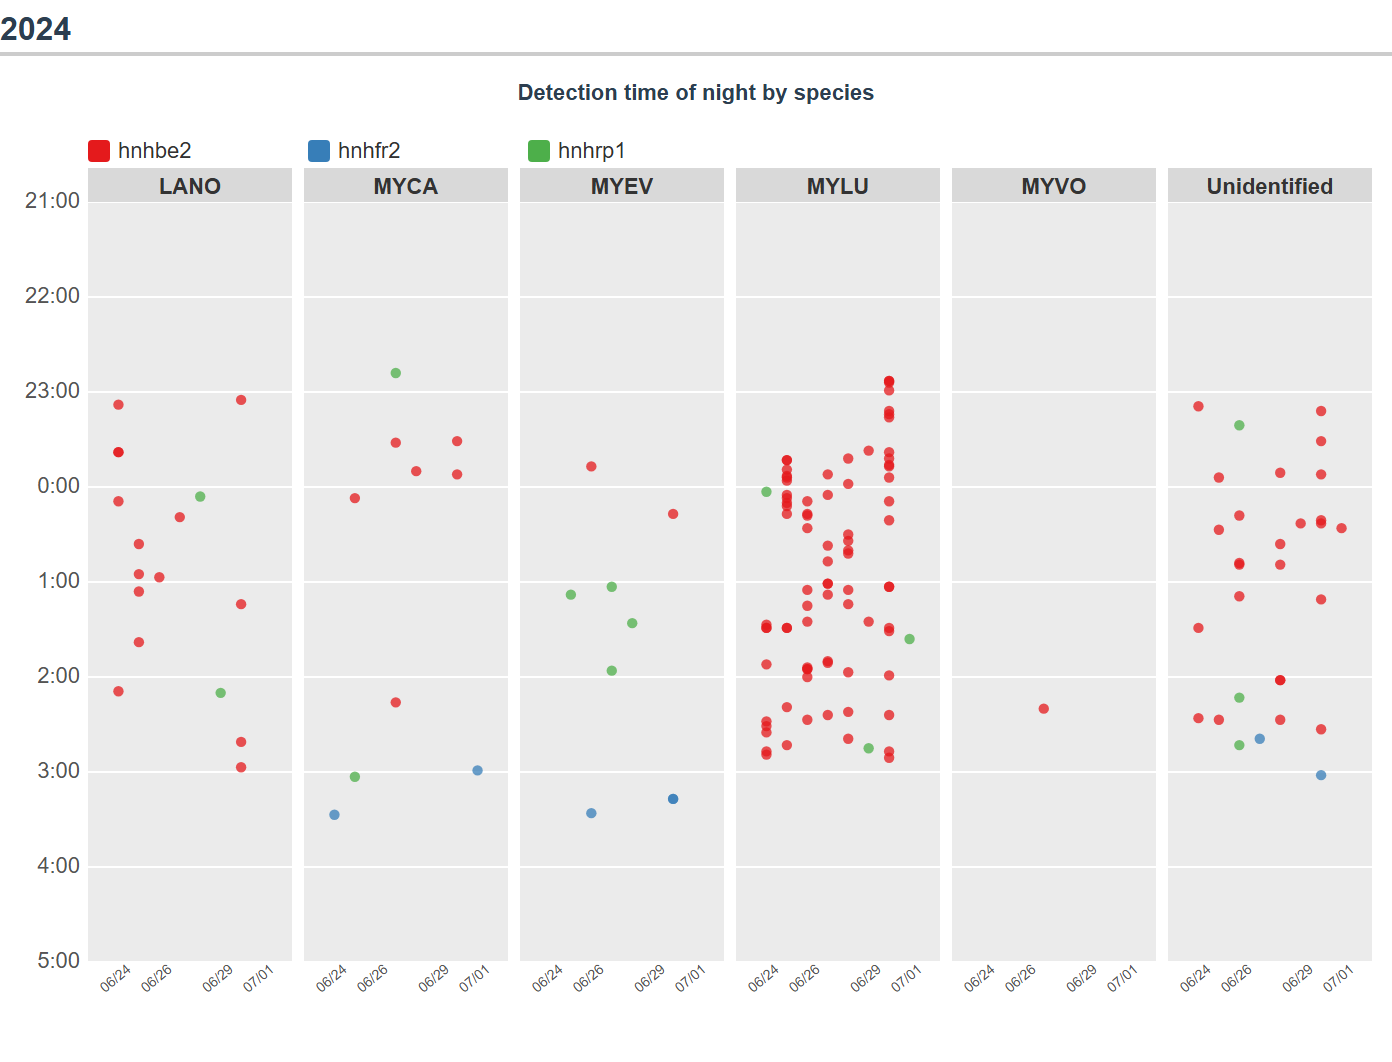
\includegraphics[width=1\linewidth,height=\textheight,keepaspectratio]{Figures/AppendixB/34254_hour.png}

}

\caption{Detection times by species and site (2025 top, 2024 below),
cell 34254 - Hoonah}

\end{figure}%

\newpage

\subsection*{Grid cell 34338 - Yakutat}\label{grid-cell-34338---yakutat}

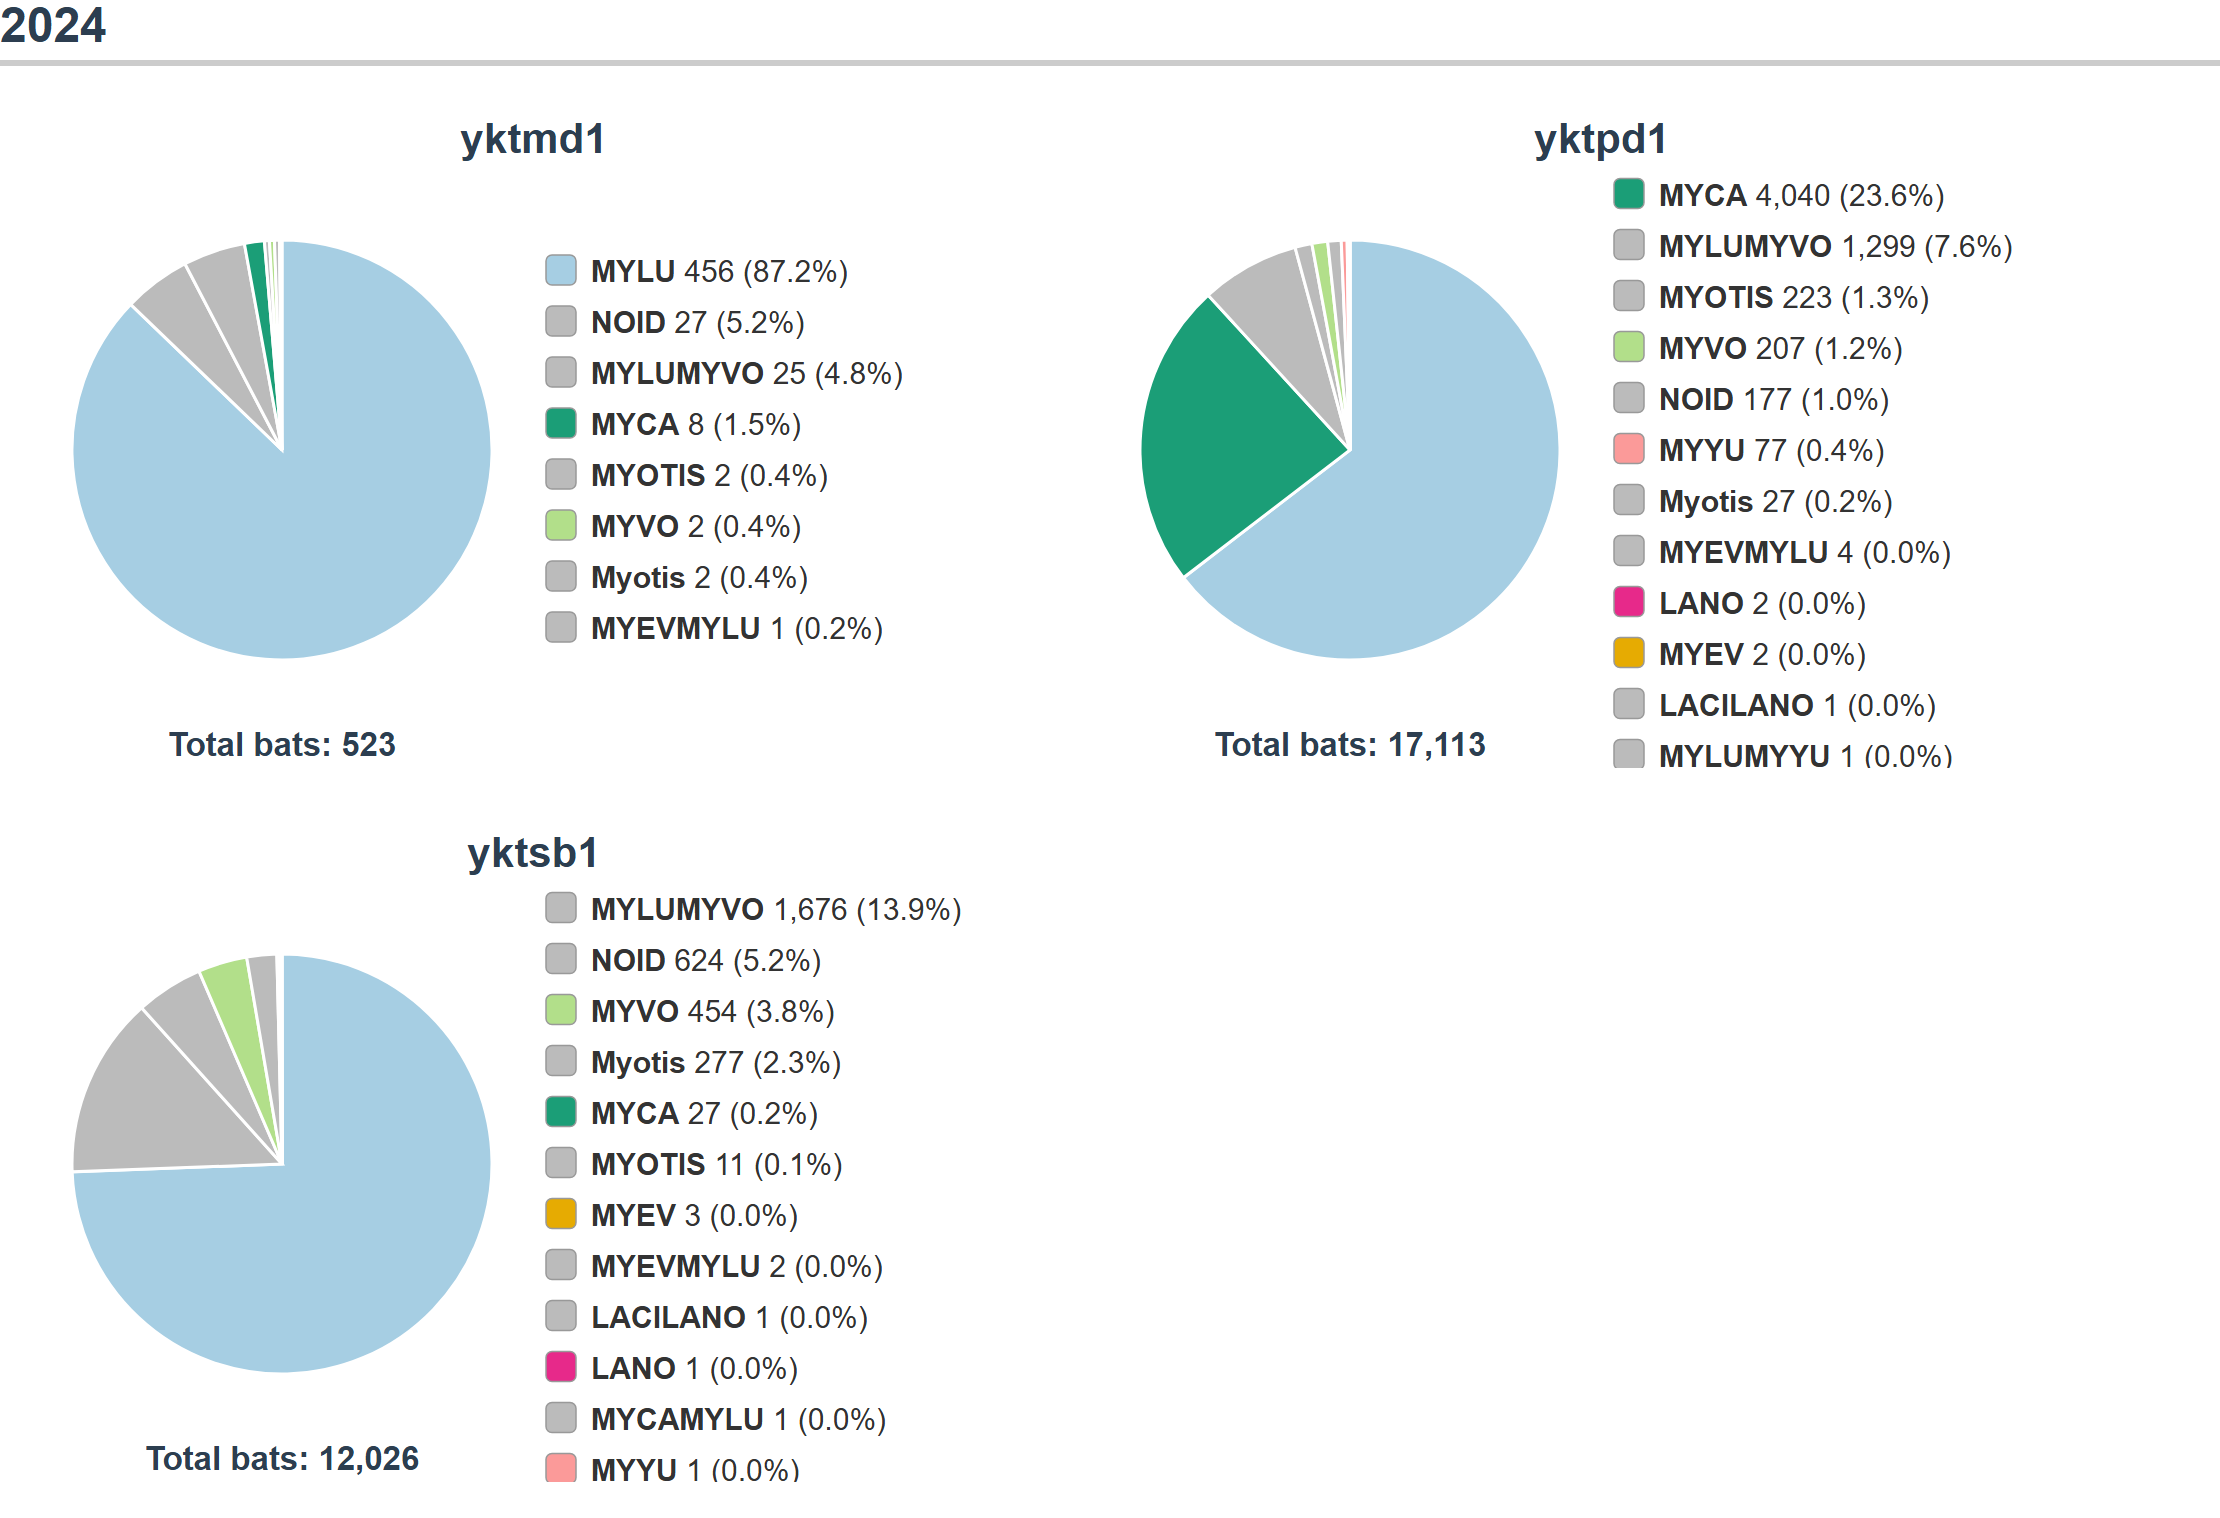
\includegraphics[width=1\linewidth,height=\textheight,keepaspectratio]{Figures/AppendixB/34338_pies.png}

\newpage

\begin{figure}[H]

{\centering 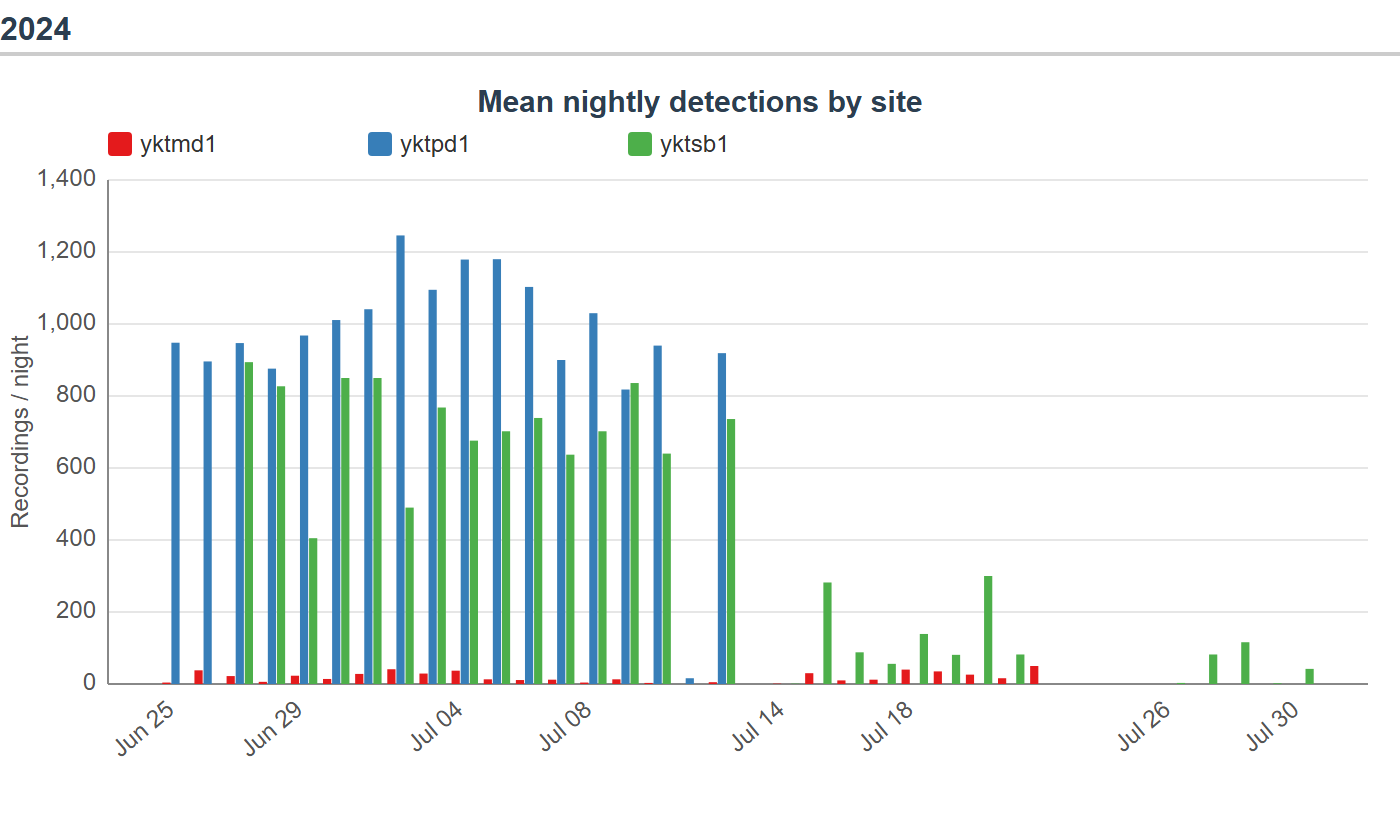
\includegraphics[width=1\linewidth,height=\textheight,keepaspectratio]{Figures/AppendixB/34338_bar.png}

}

\caption{Nightly activity by site (2025 top, 2024 below), cell 34338 -
Yakutat}

\end{figure}%

\newpage

\begin{figure}[H]

{\centering 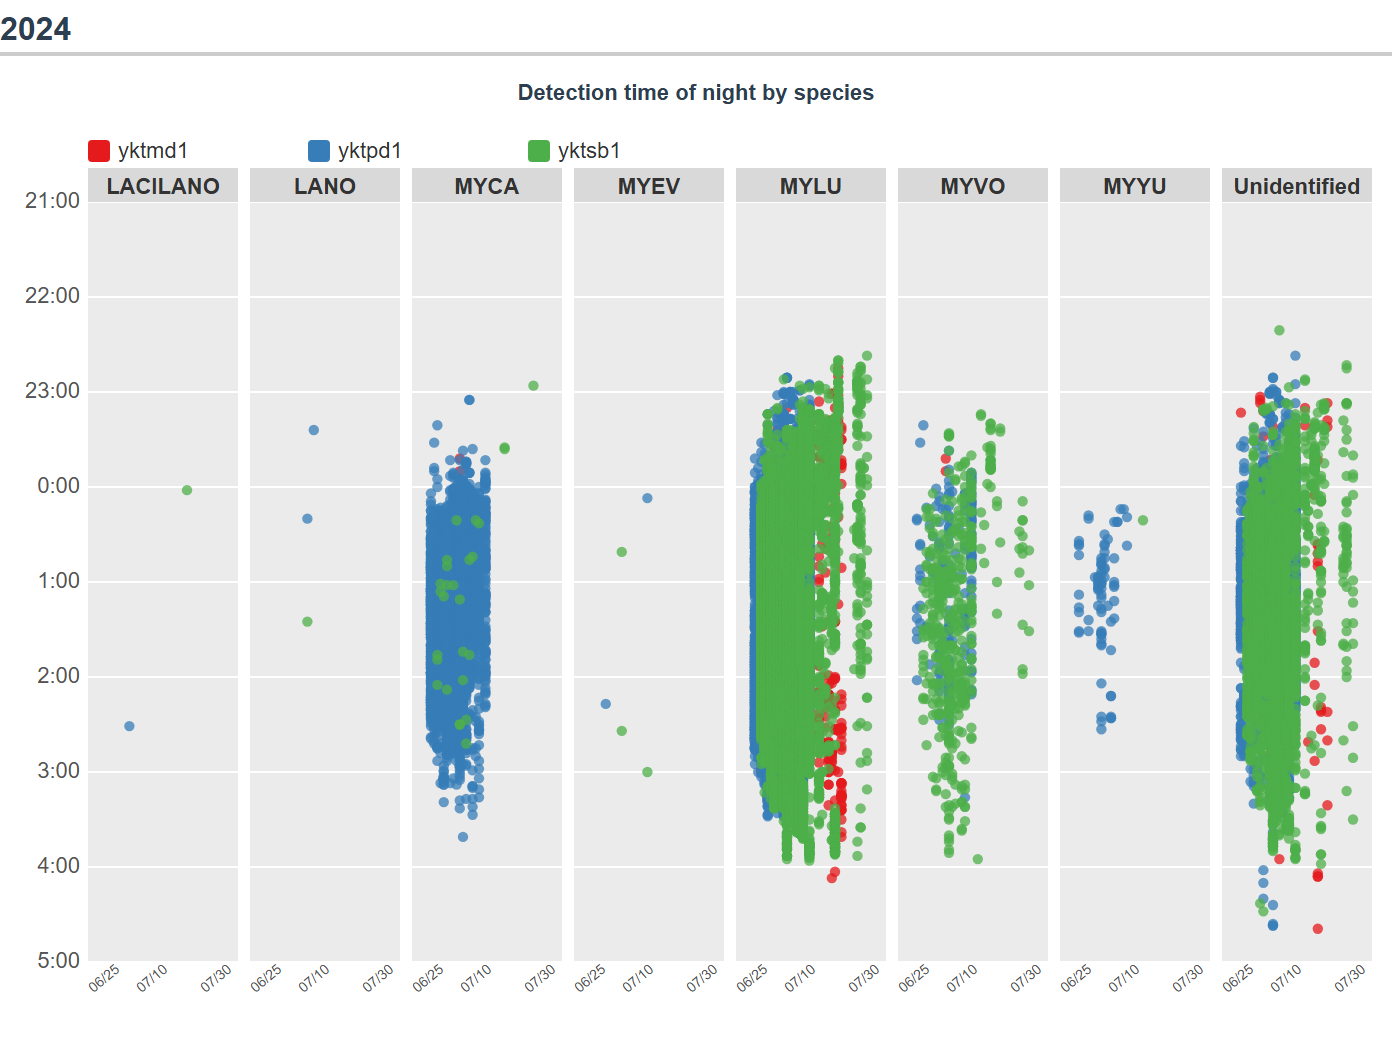
\includegraphics[width=1\linewidth,height=\textheight,keepaspectratio]{Figures/AppendixB/34338_hour.png}

}

\caption{Detection times by species and site (2025 top, 2024 below),
cell 34338 - Yakutat}

\end{figure}%

\newpage

\subsection*{Grid cell 47310 -
Ketchikan}\label{grid-cell-47310---ketchikan}

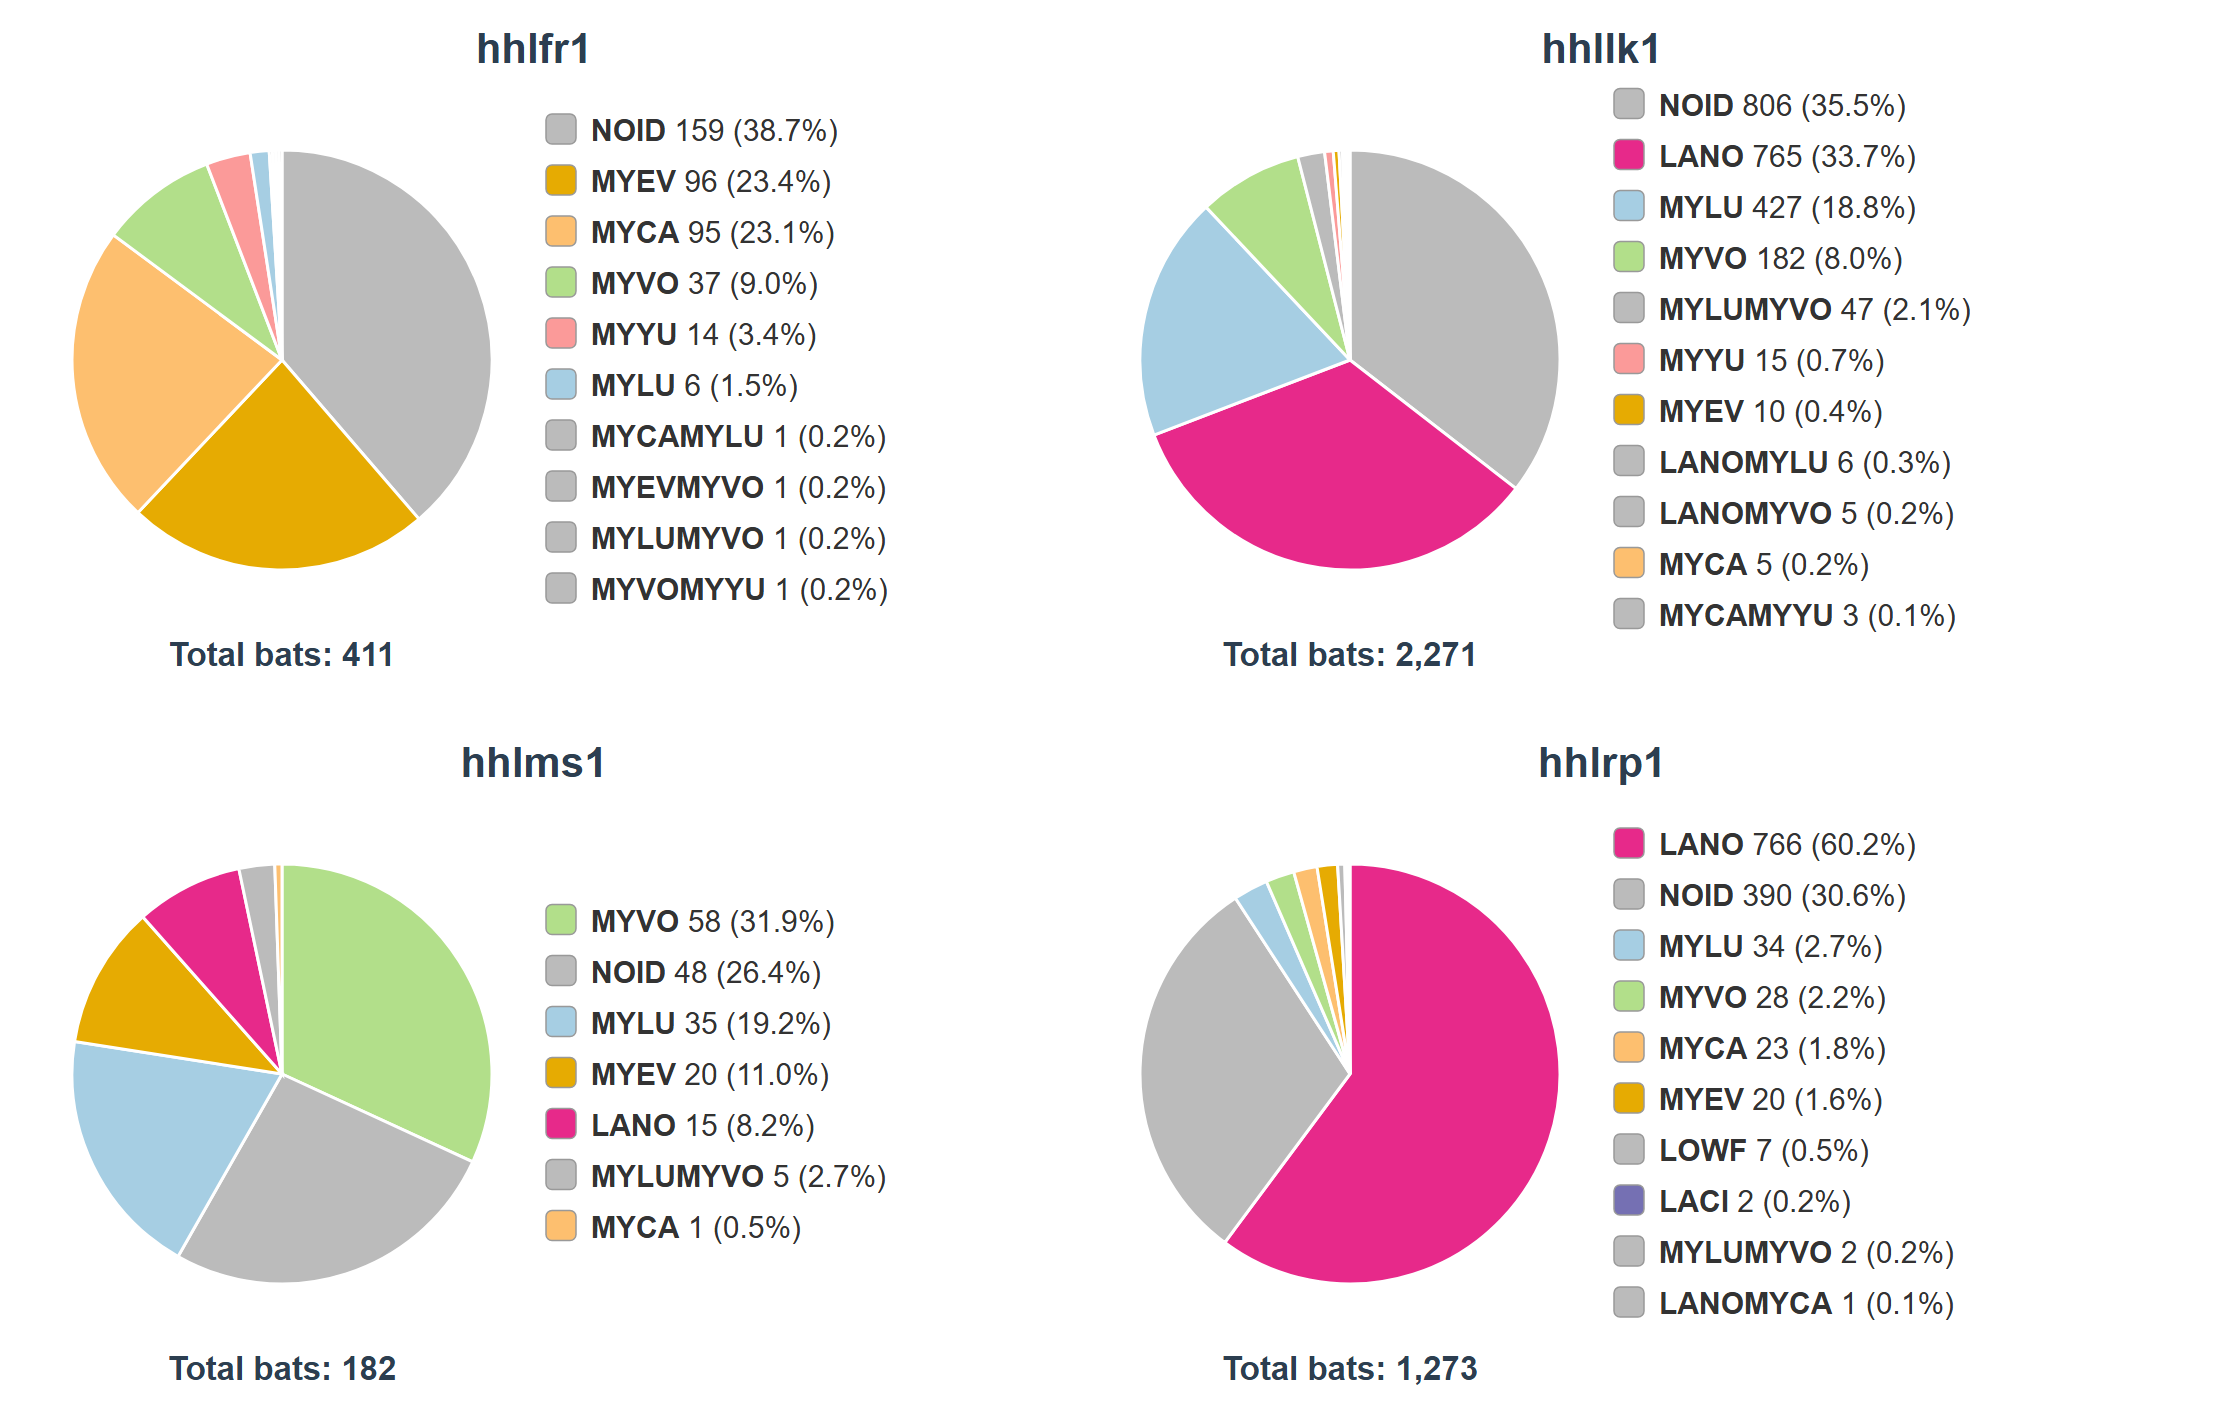
\includegraphics[width=1\linewidth,height=\textheight,keepaspectratio]{Figures/AppendixB/47310_pies.png}

\newpage

\begin{figure}[H]

{\centering 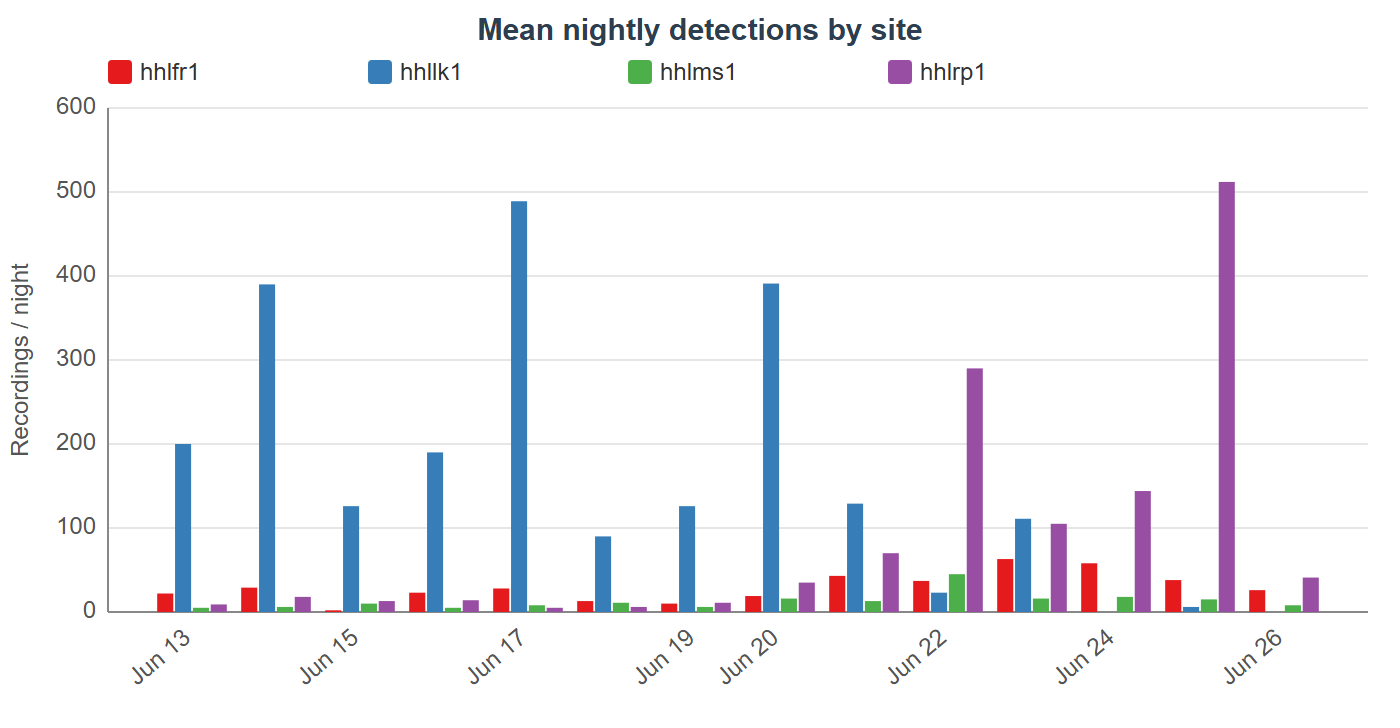
\includegraphics[width=1\linewidth,height=\textheight,keepaspectratio]{Figures/AppendixB/47310_bar.png}

}

\caption{Nightly activity by site (2025 top, 2024 below), cell 47310 -
Ketchikan}

\end{figure}%

\newpage

\begin{figure}[H]

{\centering 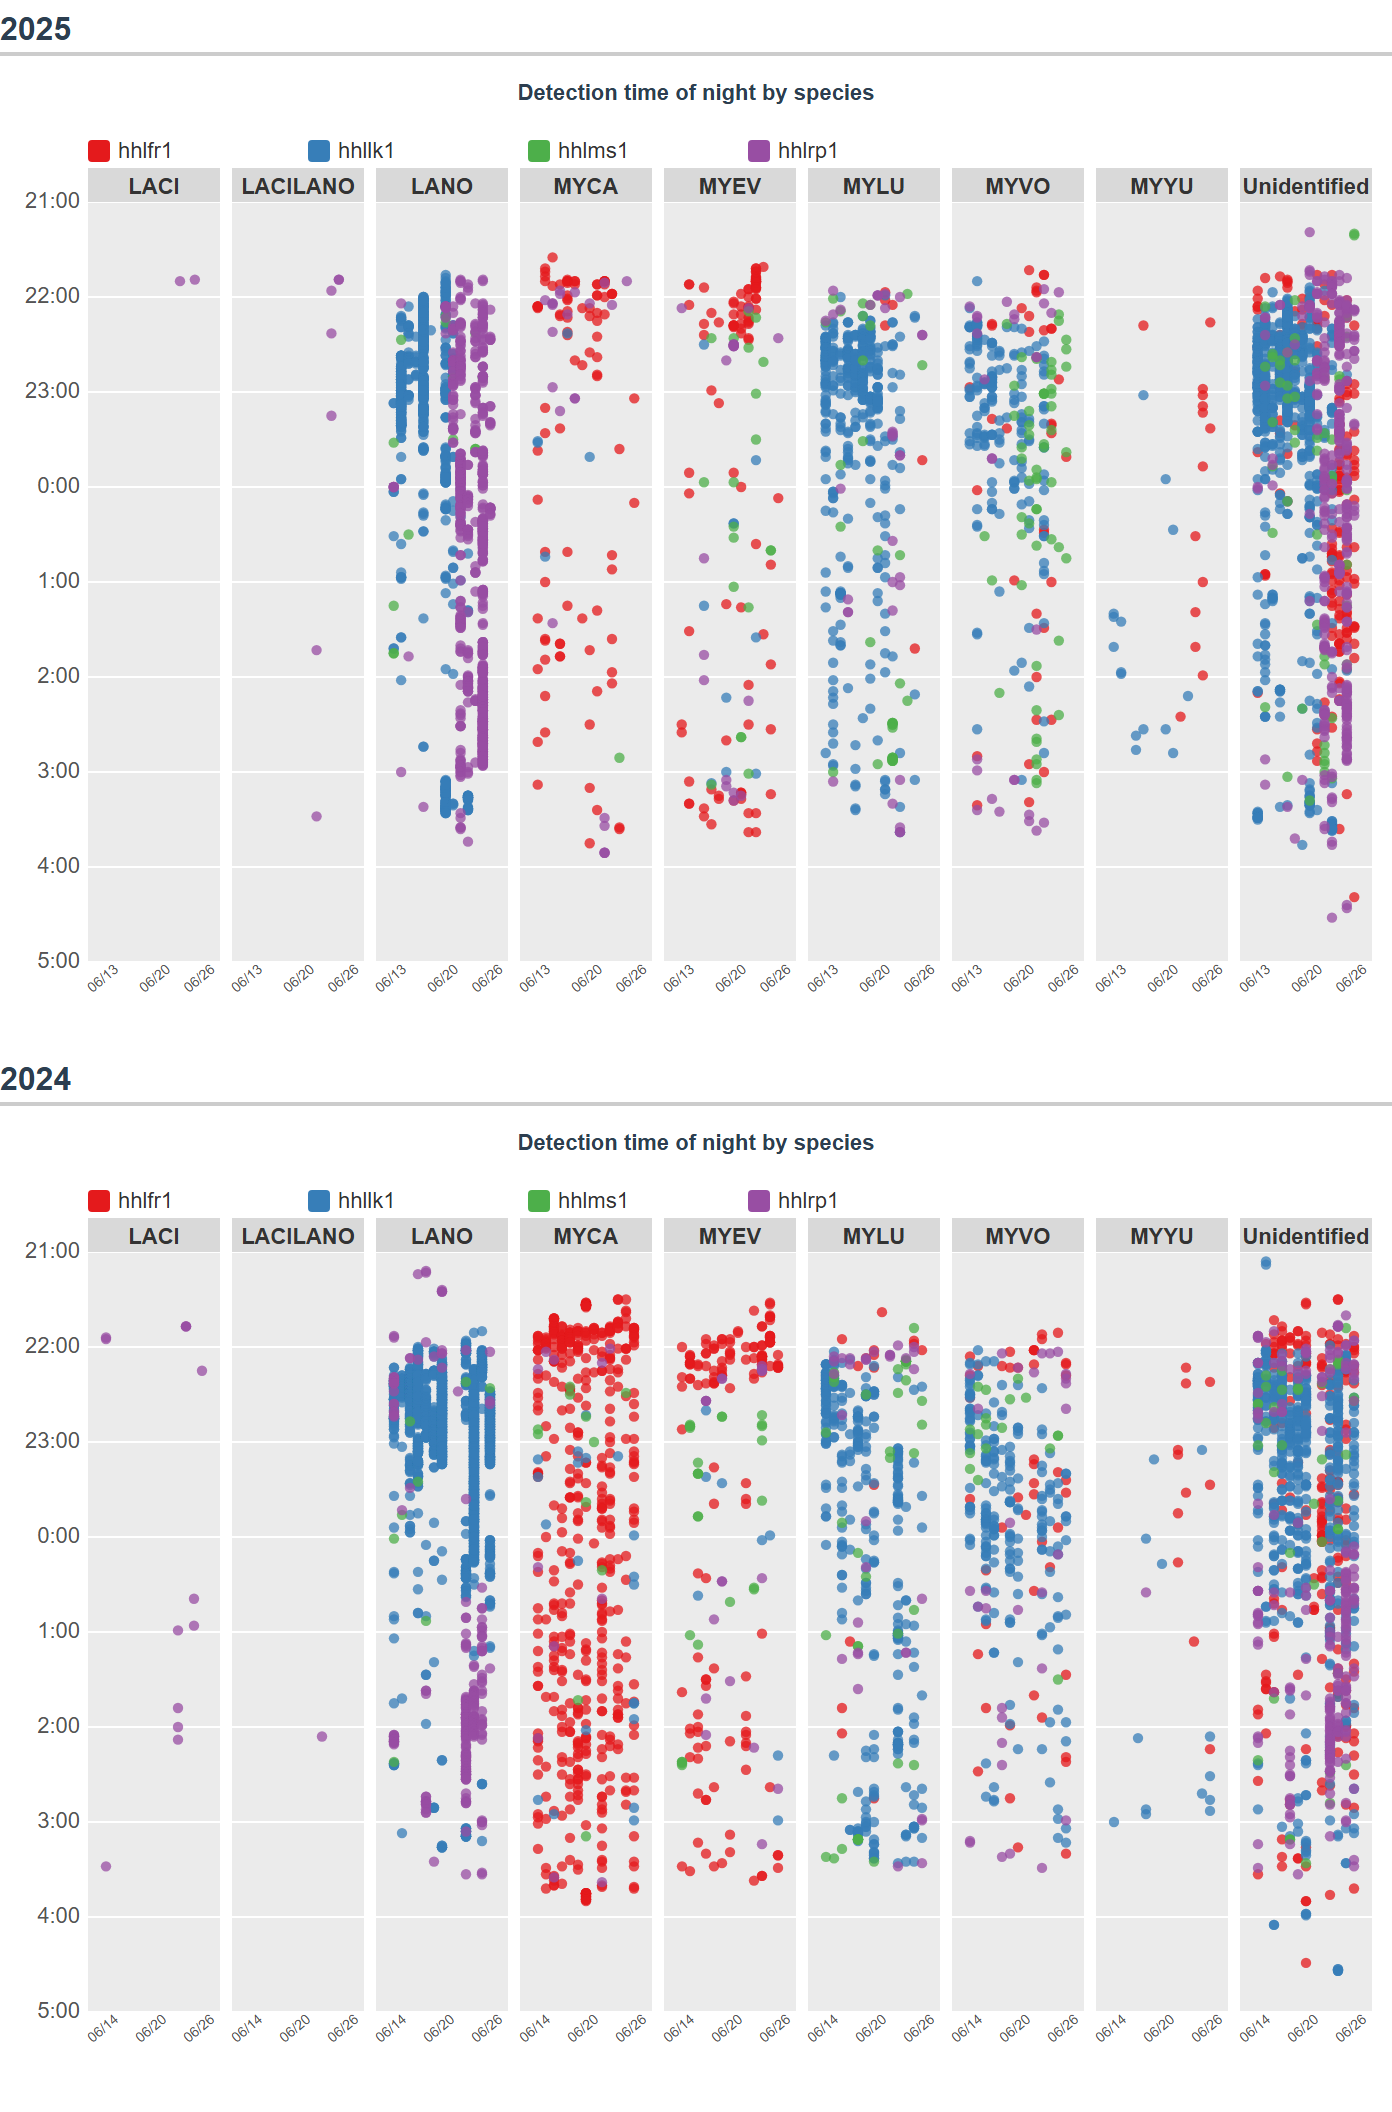
\includegraphics[width=1\linewidth,height=\textheight,keepaspectratio]{Figures/AppendixB/47310_hour.png}

}

\caption{Detection times by species and site (2025 top, 2024 below),
cell 47310 - Ketchikan}

\end{figure}%

\newpage

\subsection*{Grid cell 117173 -
Anchorage}\label{grid-cell-117173---anchorage}

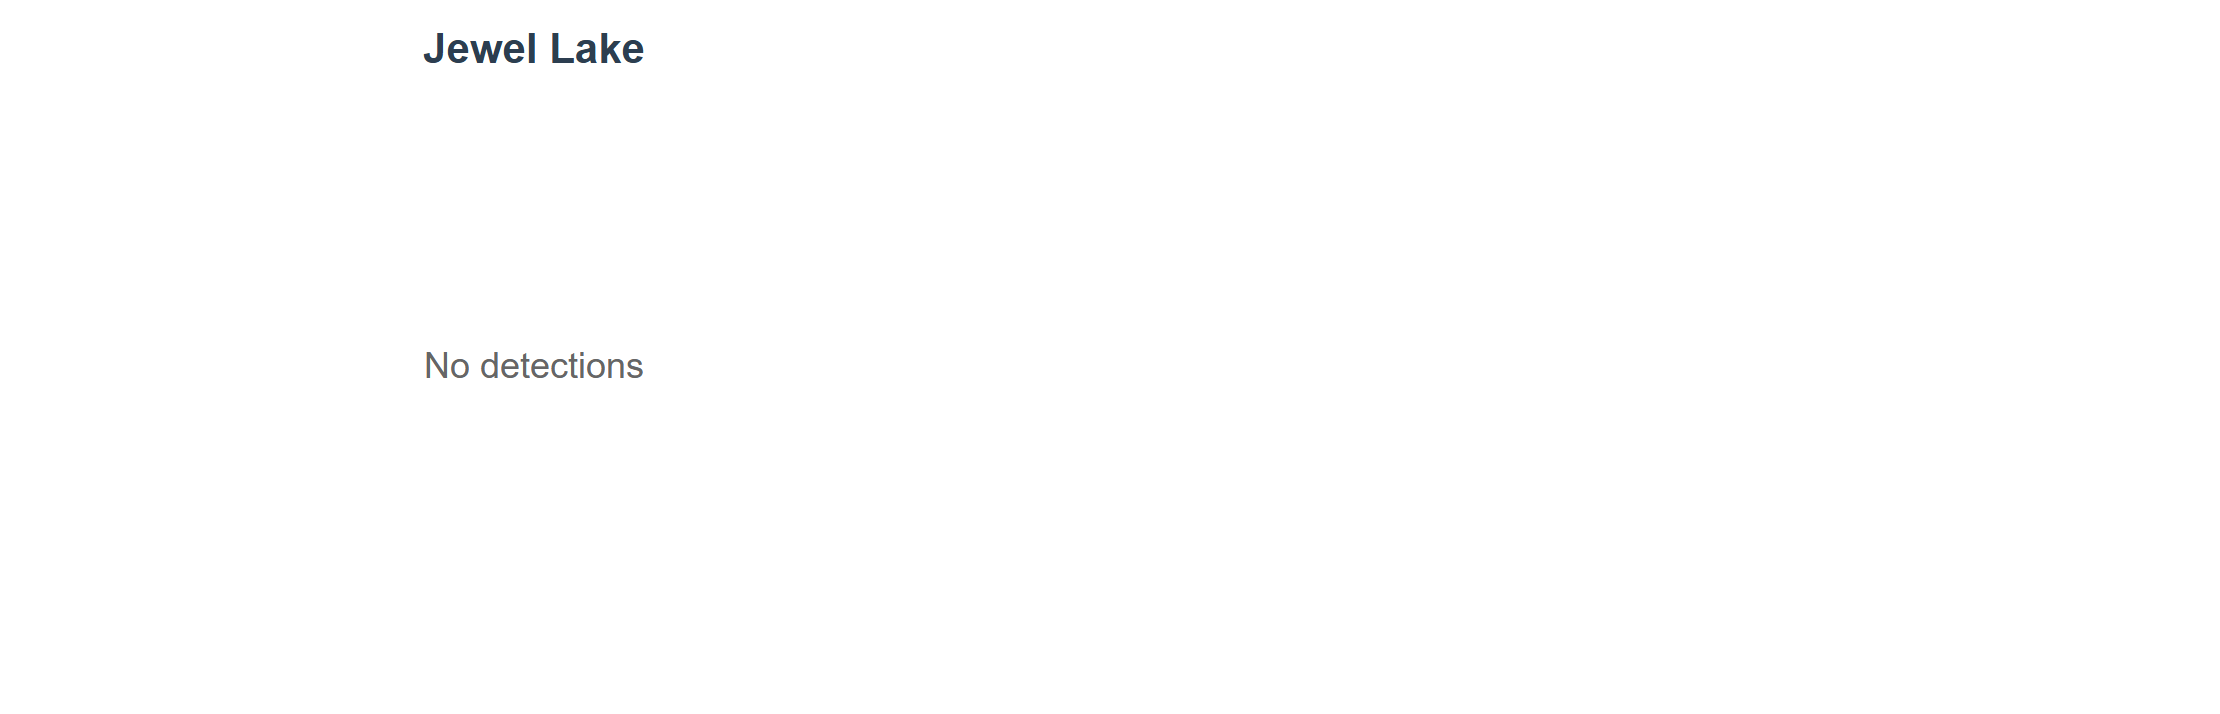
\includegraphics[width=1\linewidth,height=\textheight,keepaspectratio]{Figures/AppendixB/117173_pies.png}

\newpage

\begin{figure}[H]

{\centering 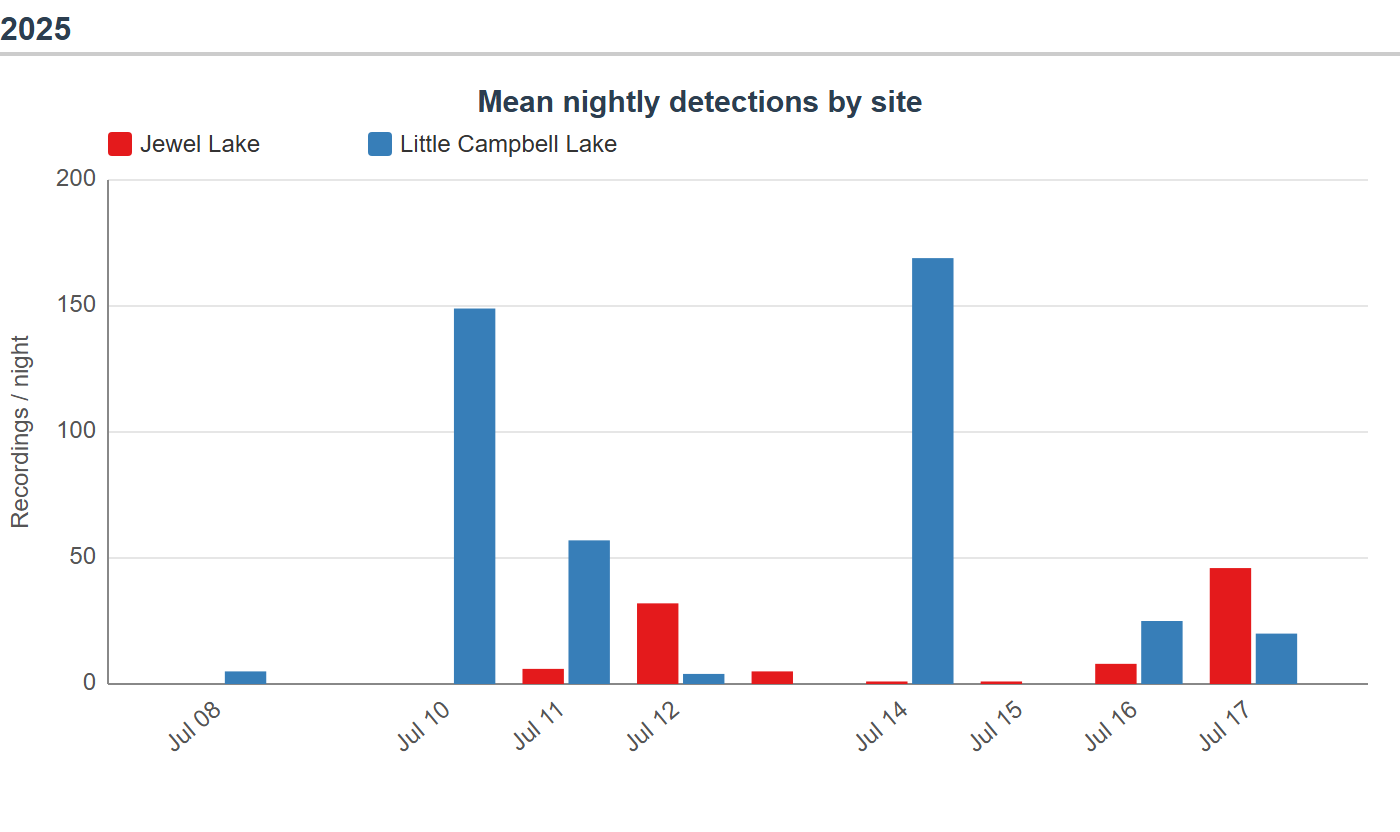
\includegraphics[width=1\linewidth,height=\textheight,keepaspectratio]{Figures/AppendixB/117173_bar.png}

}

\caption{Nightly activity by site (2025 top, 2024 below), cell 117173 -
Anchorage}

\end{figure}%

\newpage

\begin{figure}[H]

{\centering 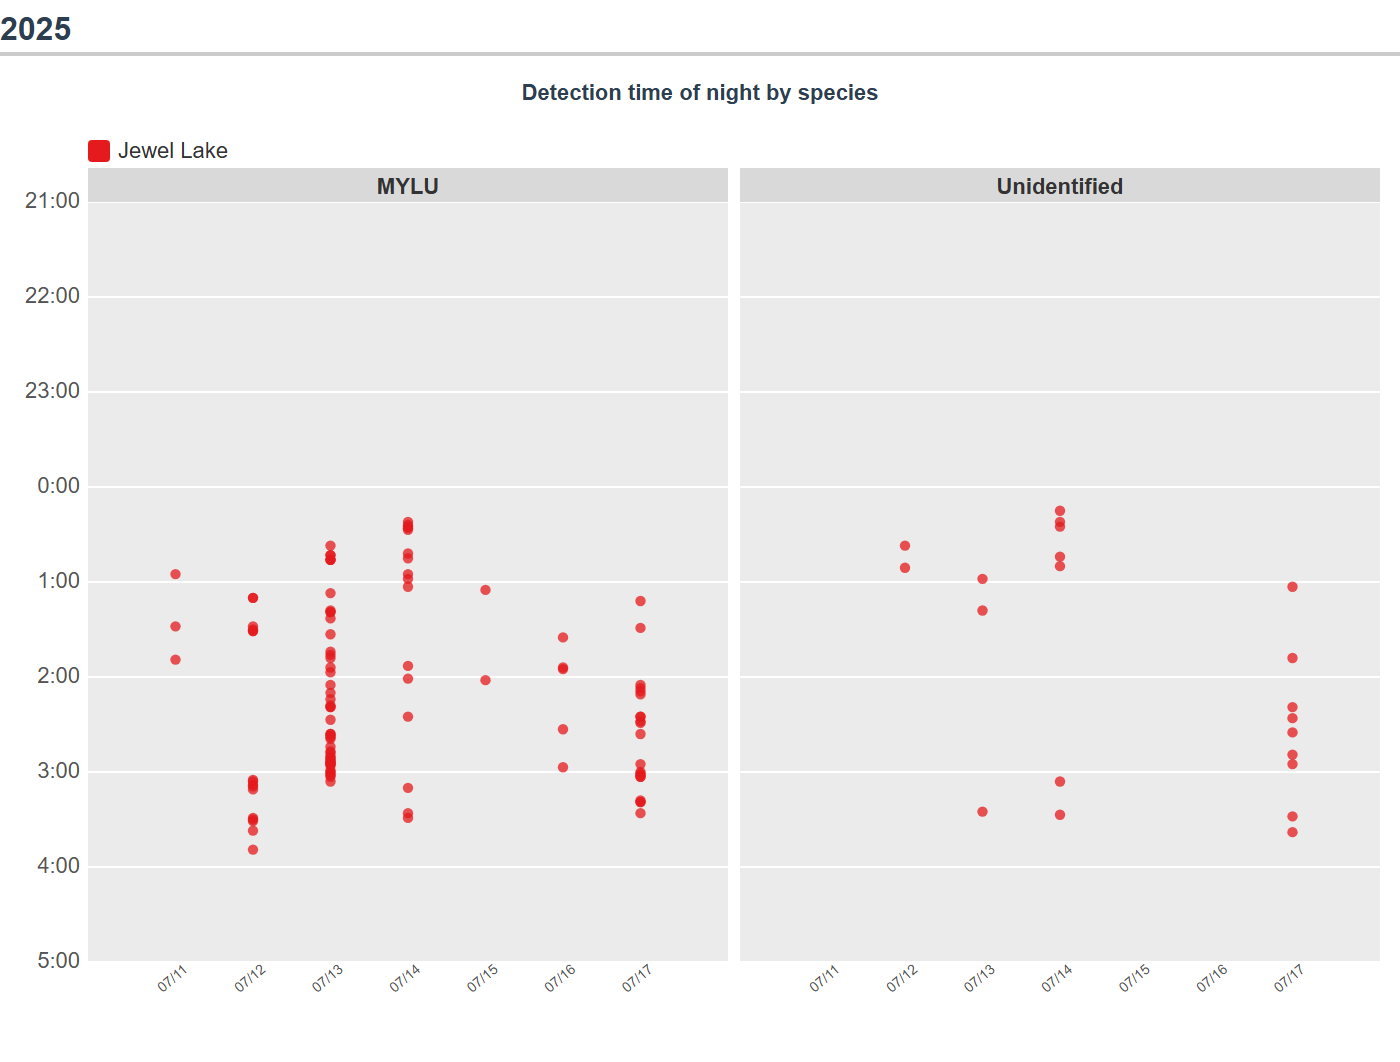
\includegraphics[width=1\linewidth,height=\textheight,keepaspectratio]{Figures/AppendixB/117173_hour.png}

}

\caption{Detection times by species and site (2025 top, 2024 below),
cell 117173 - Anchorage}

\end{figure}%

\newpage

\subsection*{Grid cell 154037 -
Anchorage}\label{grid-cell-154037---anchorage}

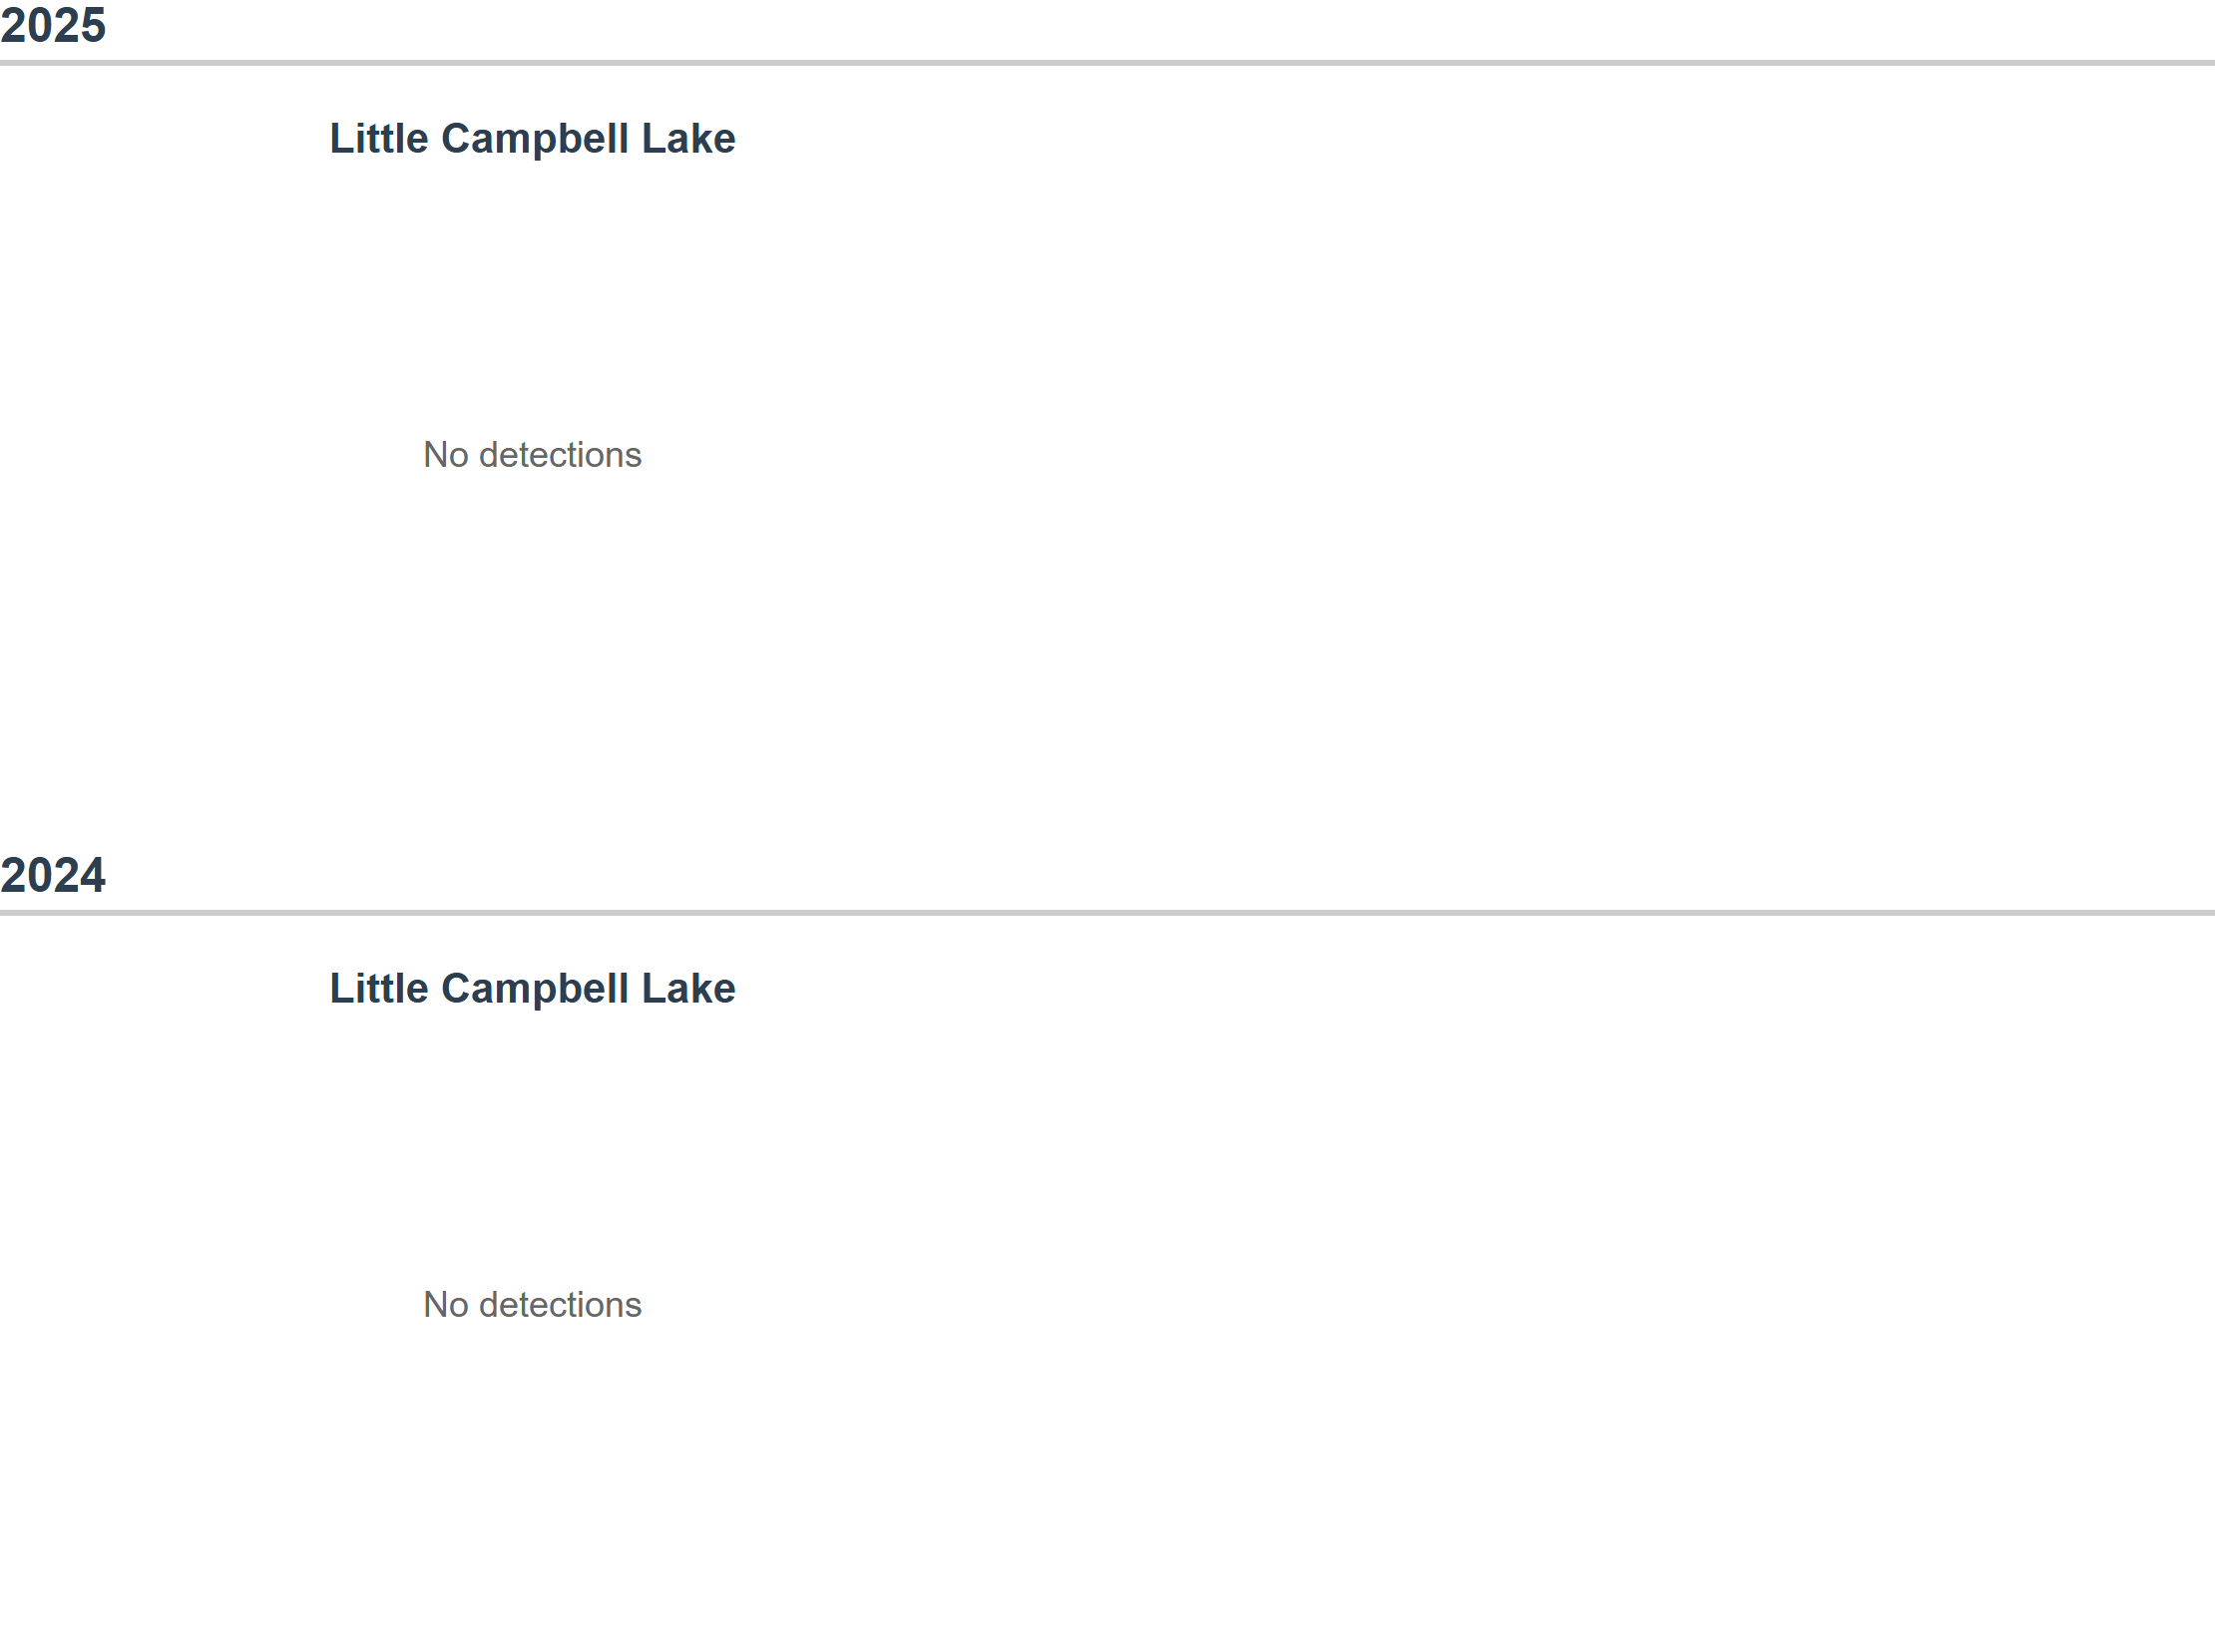
\includegraphics[width=1\linewidth,height=\textheight,keepaspectratio]{Figures/AppendixB/154037_pies.png}

\newpage

\begin{figure}[H]

{\centering 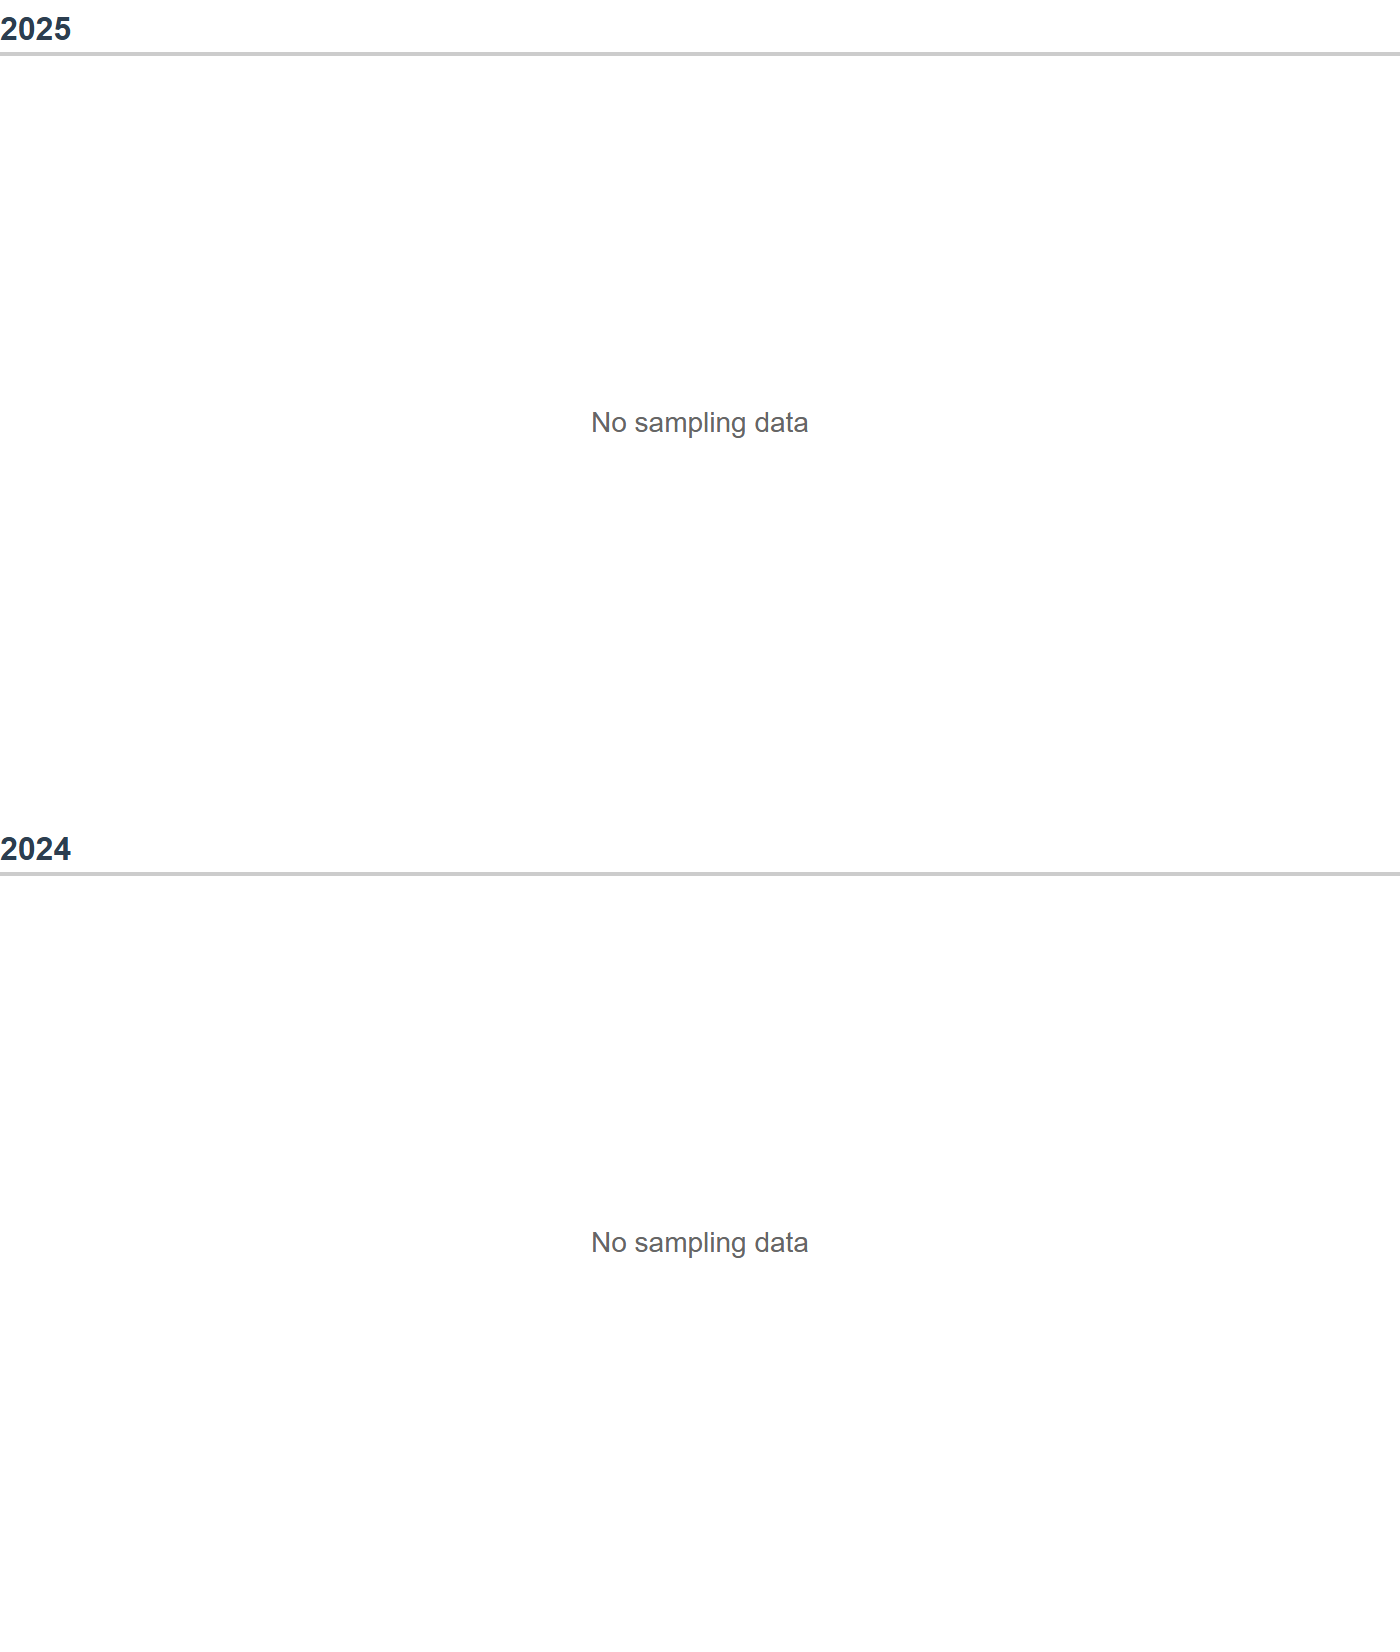
\includegraphics[width=1\linewidth,height=\textheight,keepaspectratio]{Figures/AppendixB/154037_bar.png}

}

\caption{Nightly activity by site (2025 top, 2024 below), cell 154037 -
Anchorage}

\end{figure}%

\newpage

\begin{figure}[H]

{\centering 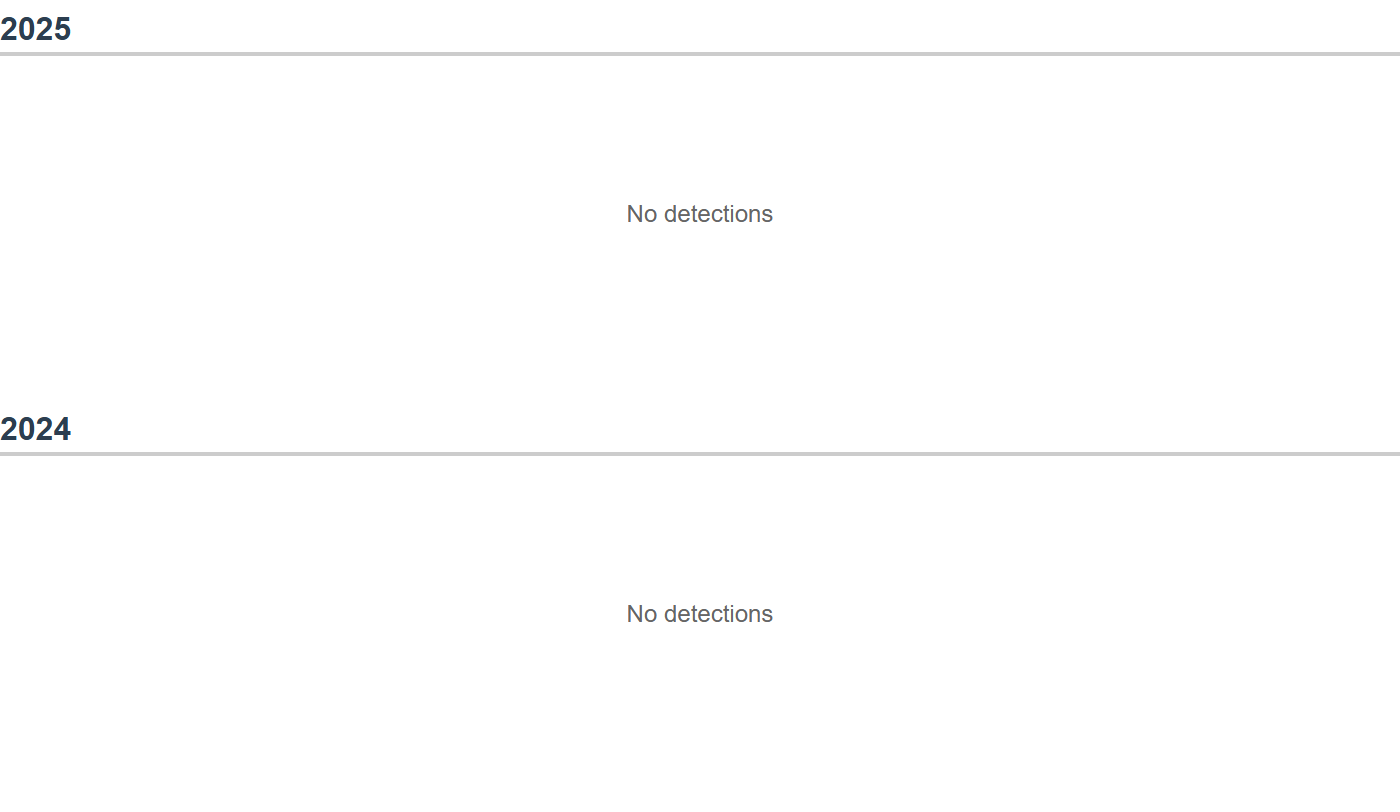
\includegraphics[width=1\linewidth,height=\textheight,keepaspectratio]{Figures/AppendixB/154037_hour.png}

}

\caption{Detection times by species and site (2025 top, 2024 below),
cell 154037 - Anchorage}

\end{figure}%

\newpage

\subsection*{Grid cell 203189 -
Anchorage}\label{grid-cell-203189---anchorage}

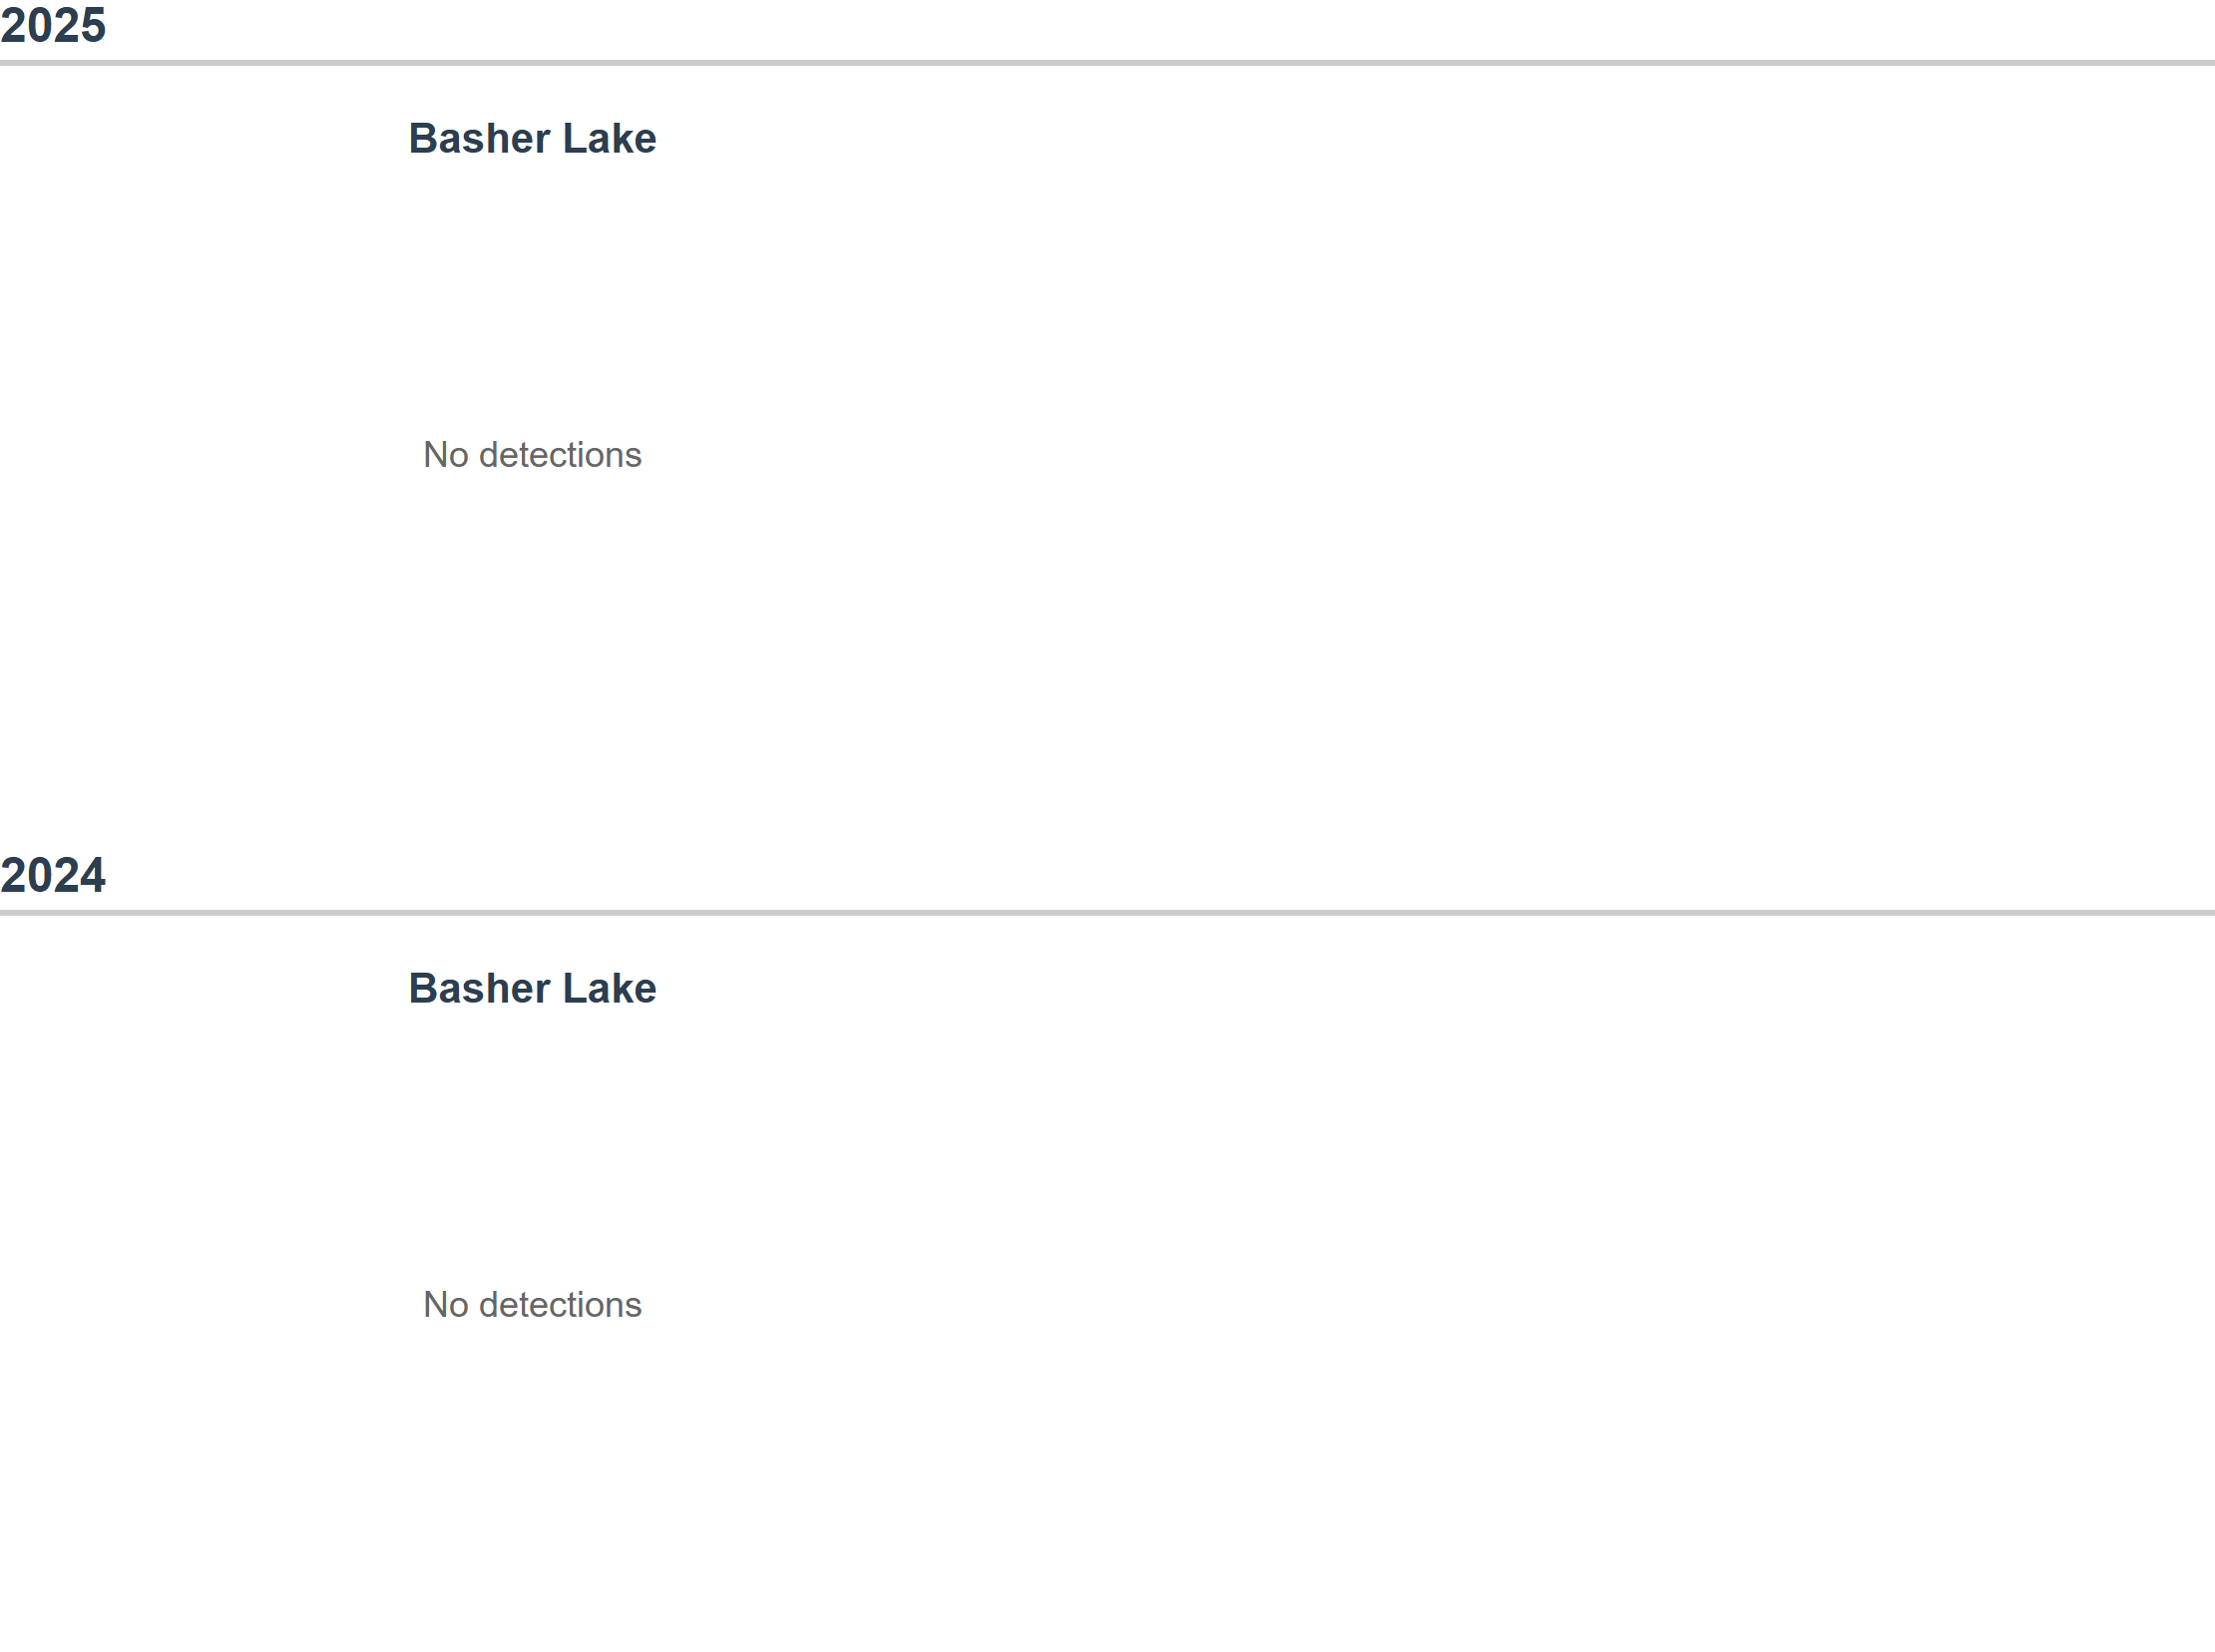
\includegraphics[width=1\linewidth,height=\textheight,keepaspectratio]{Figures/AppendixB/203189_pies.png}

\newpage

\begin{figure}[H]

{\centering 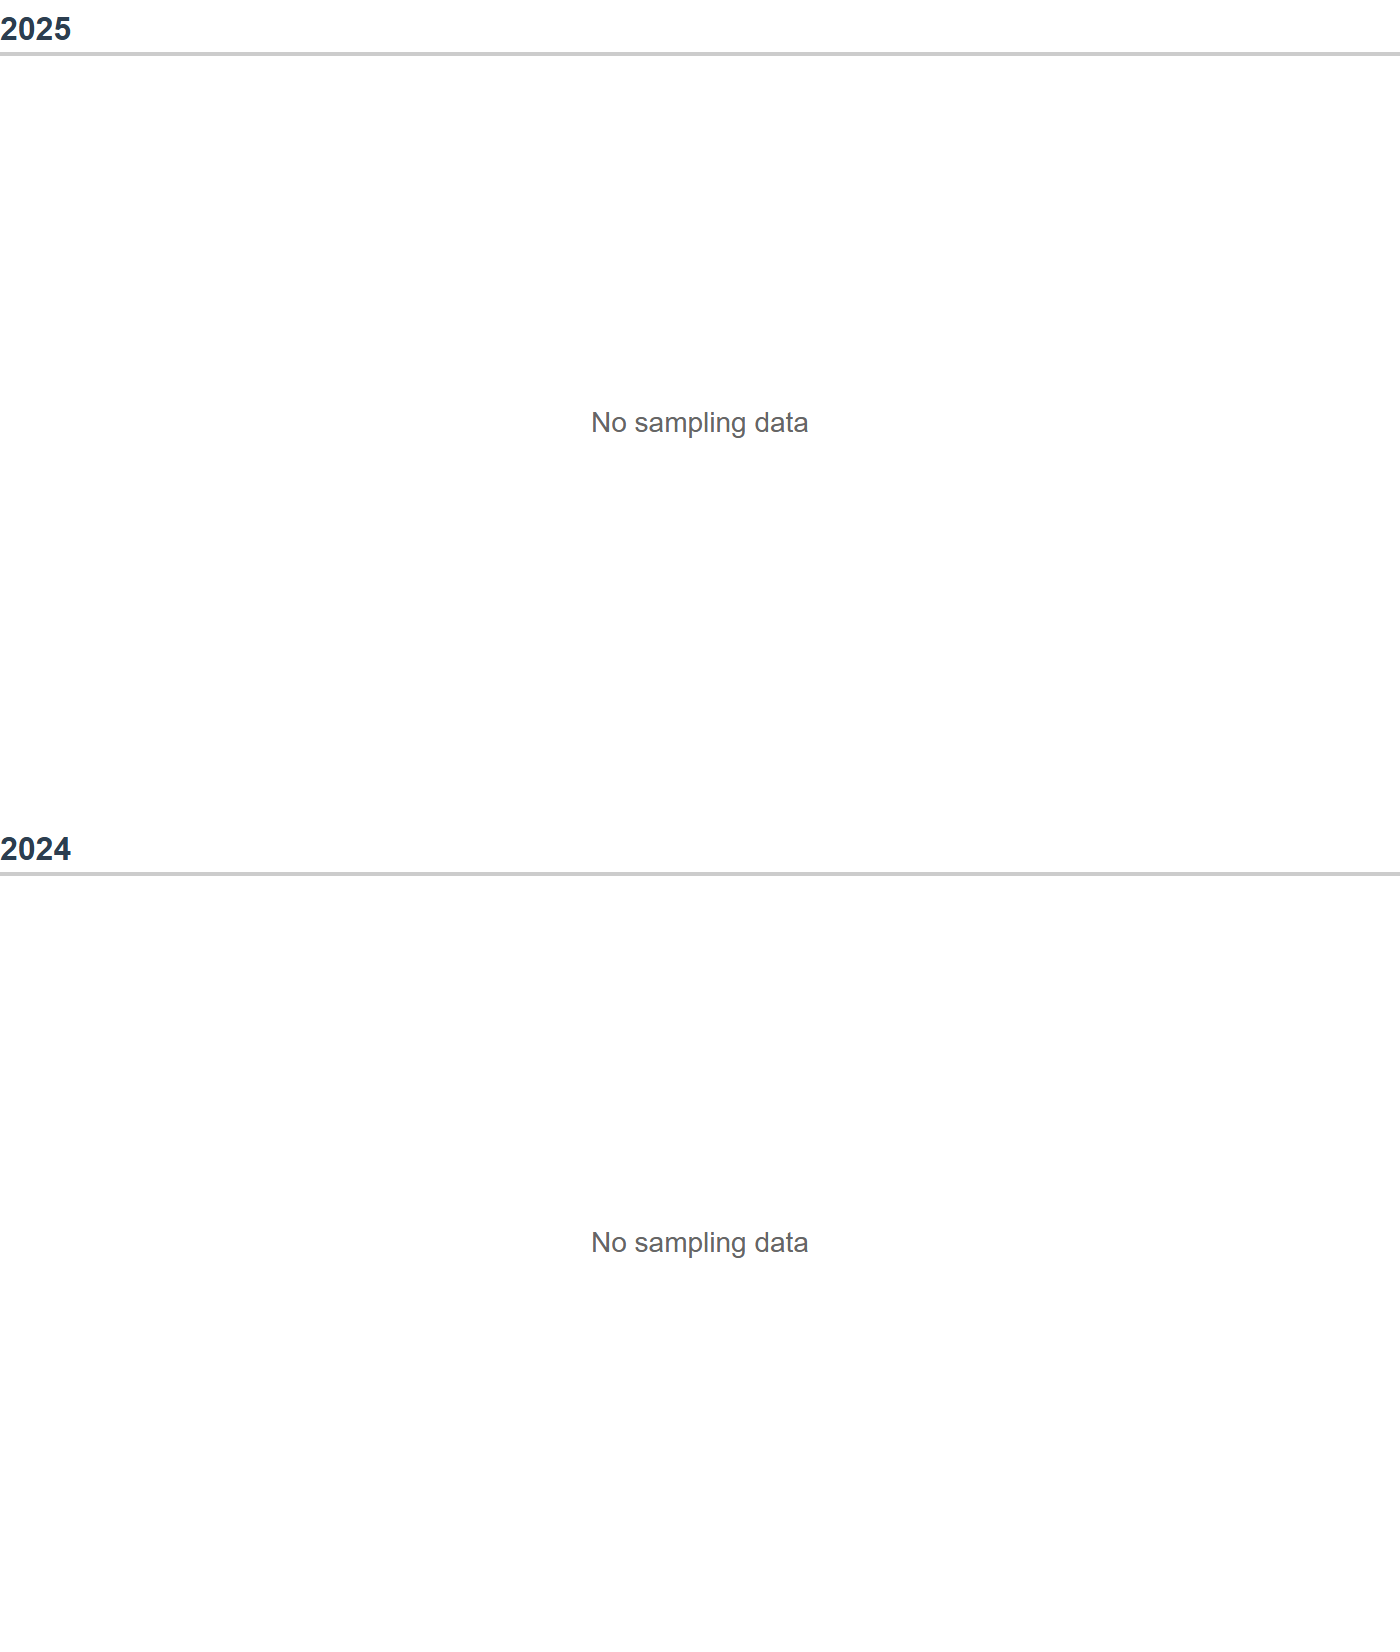
\includegraphics[width=1\linewidth,height=\textheight,keepaspectratio]{Figures/AppendixB/203189_bar.png}

}

\caption{Nightly activity by site (2025 top, 2024 below), cell 203189 -
Anchorage}

\end{figure}%

\newpage

\begin{figure}[H]

{\centering 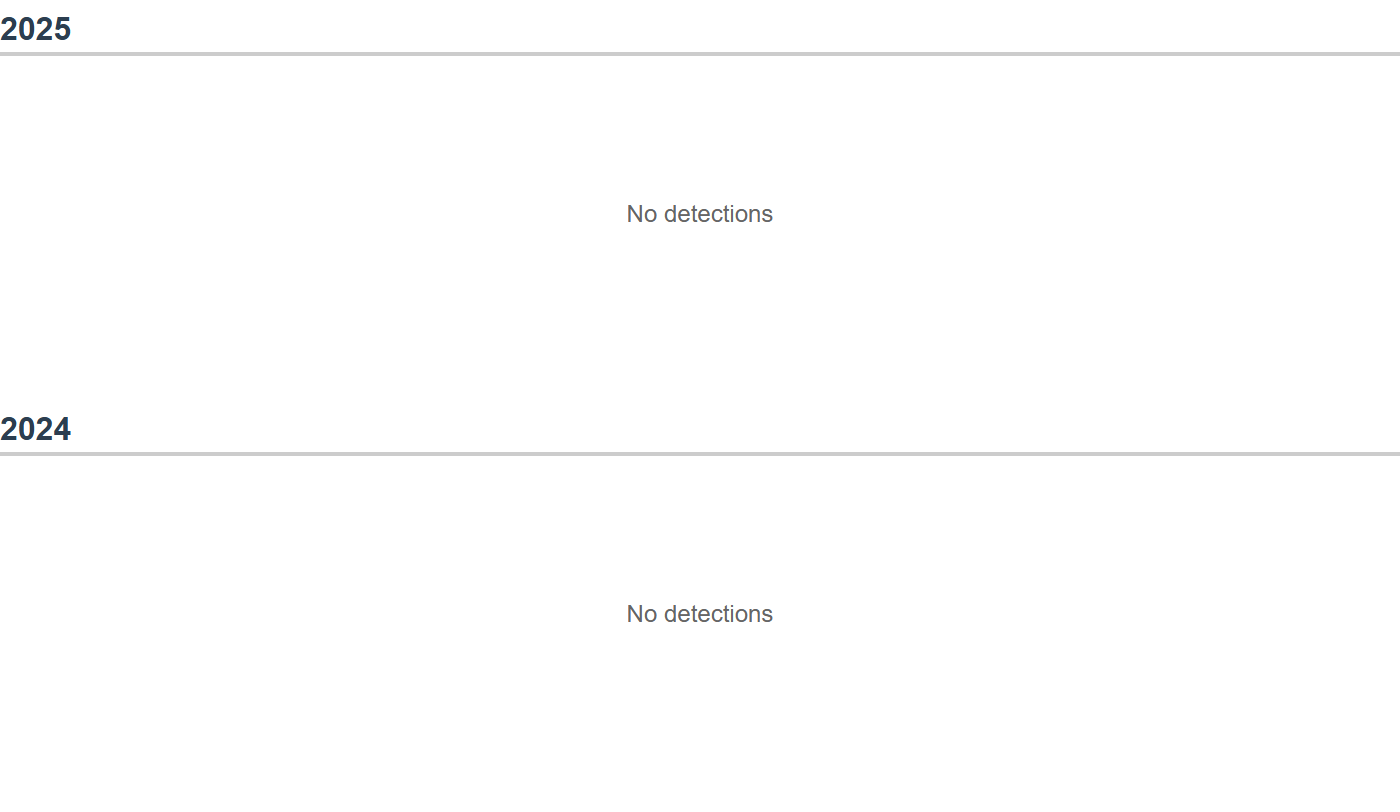
\includegraphics[width=1\linewidth,height=\textheight,keepaspectratio]{Figures/AppendixB/203189_hour.png}

}

\caption{Detection times by species and site (2025 top, 2024 below),
cell 203189 - Anchorage}

\end{figure}%

\newpage

\subsection*{Grid cell 315563 - Valley}\label{grid-cell-315563---valley}

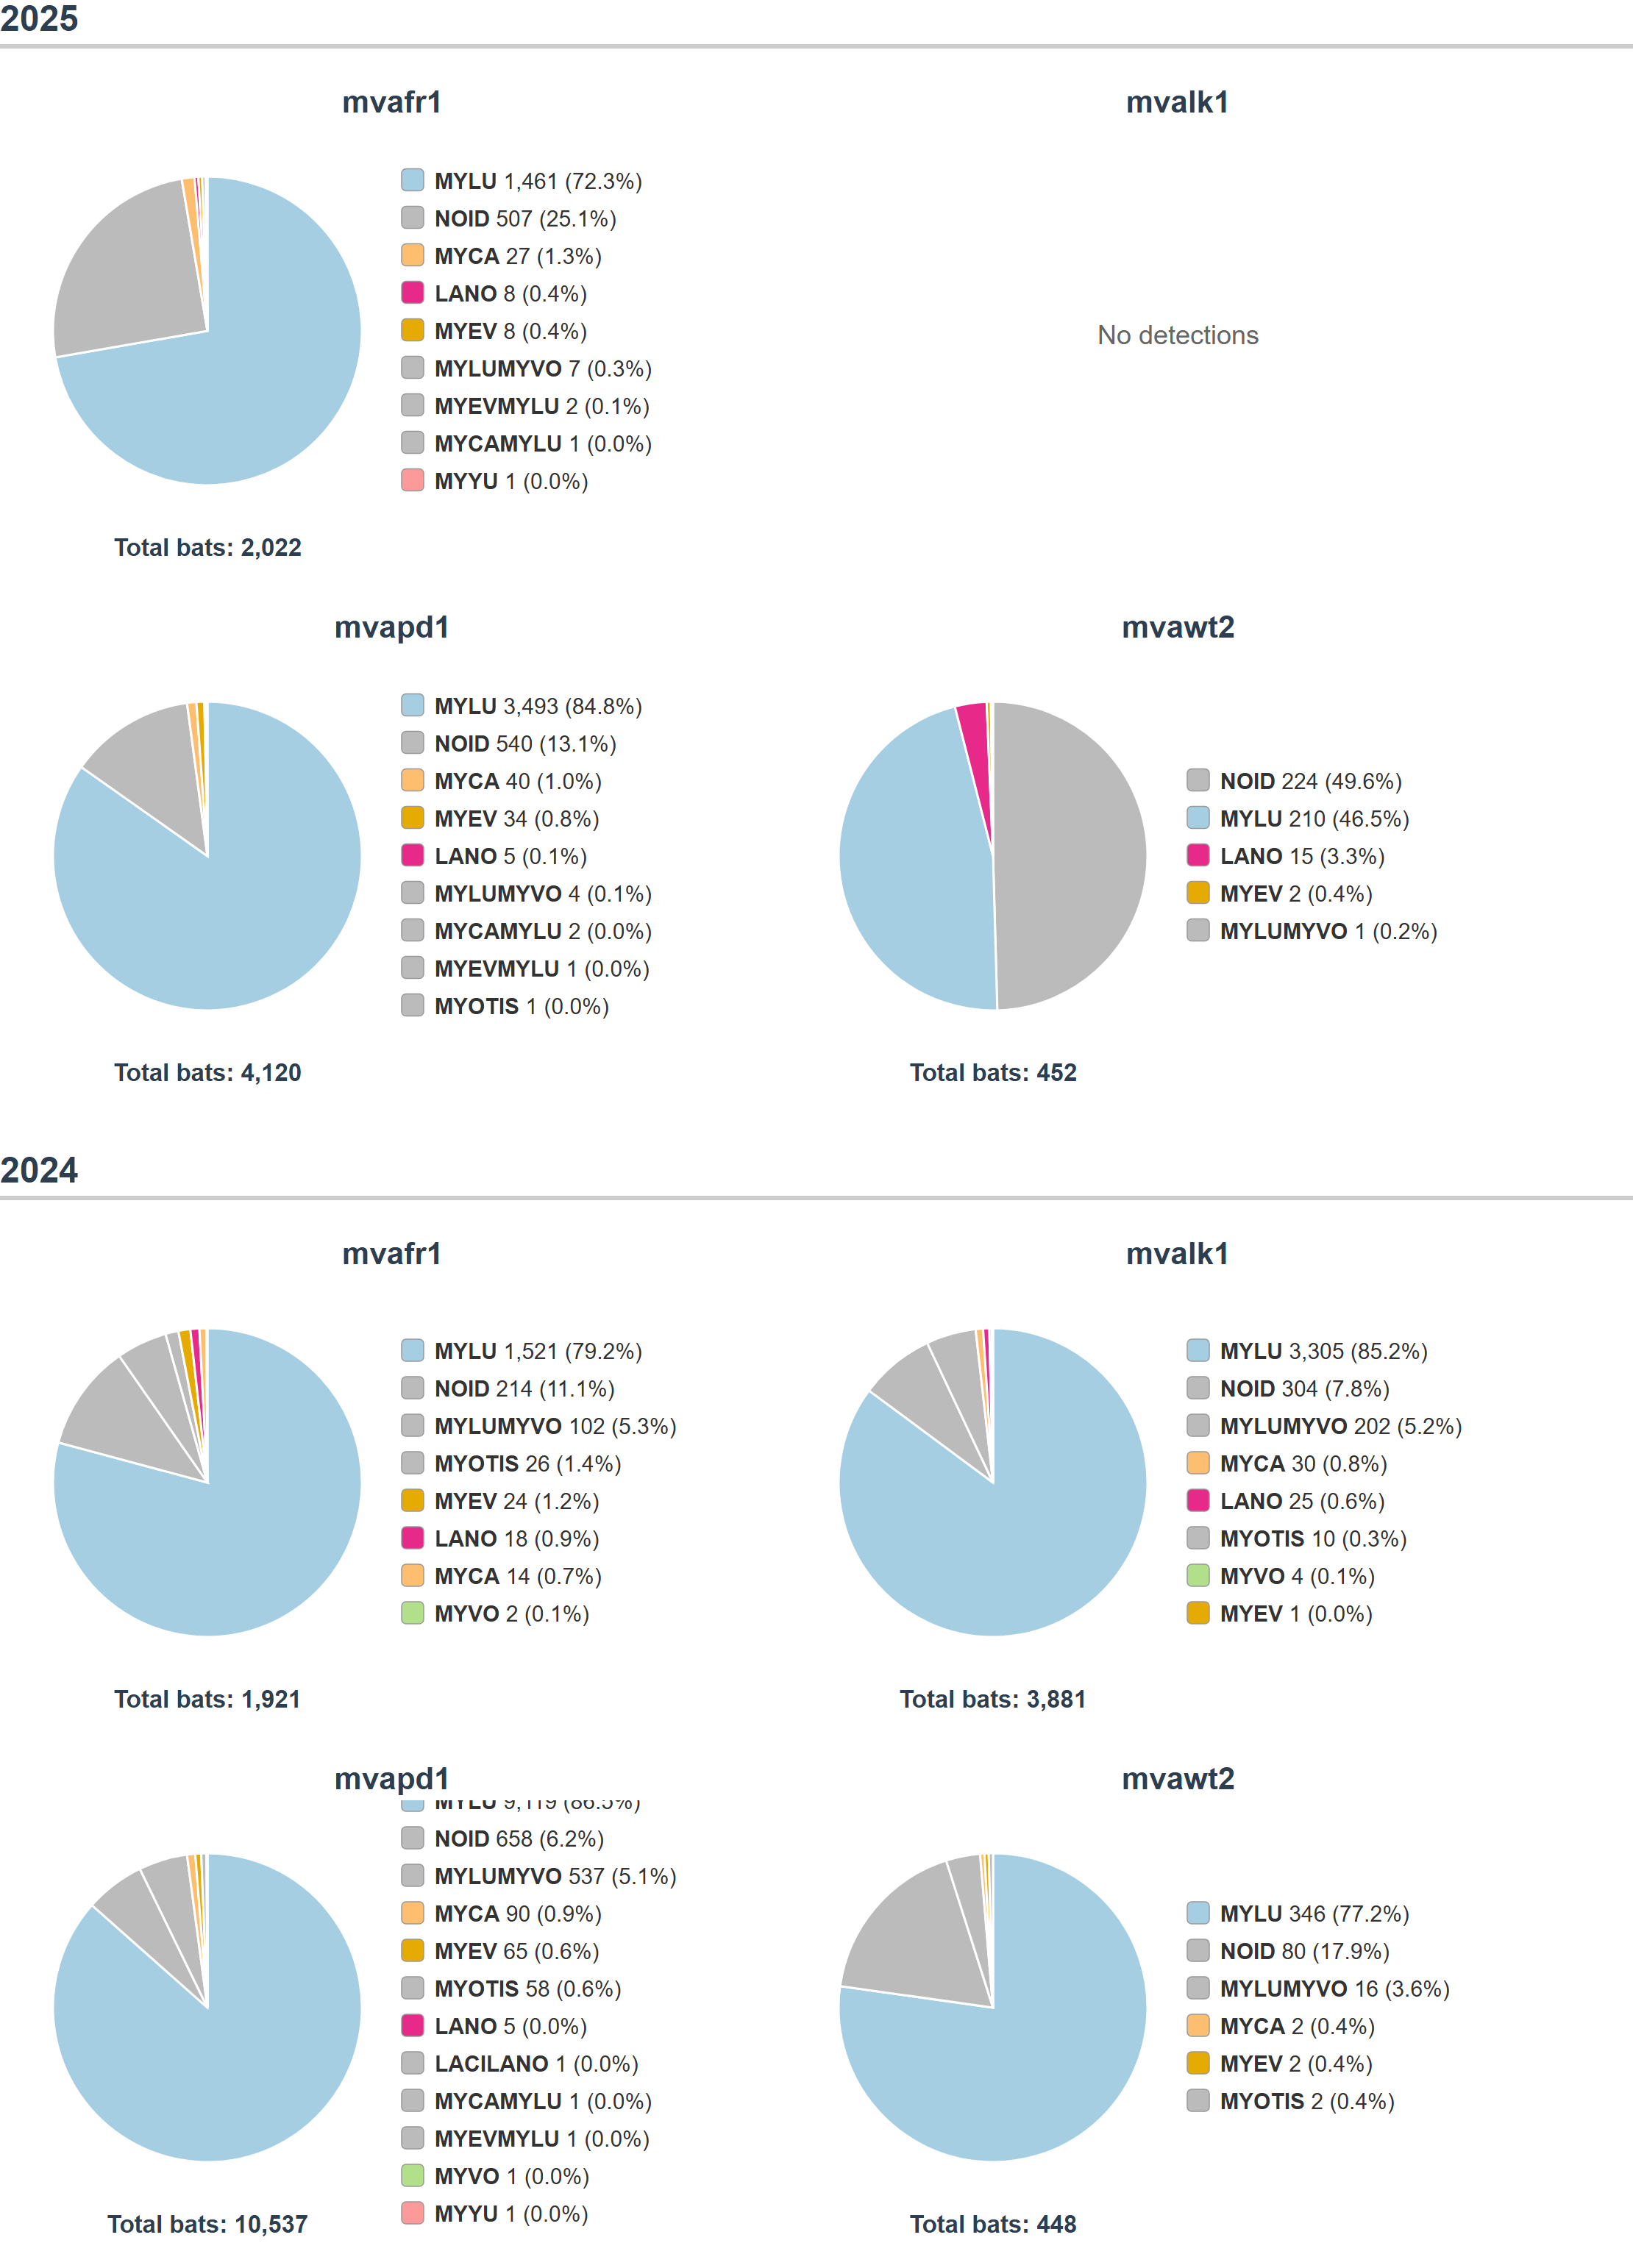
\includegraphics[width=1\linewidth,height=\textheight,keepaspectratio]{Figures/AppendixB/315563_pies.png}

\newpage

\begin{figure}[H]

{\centering 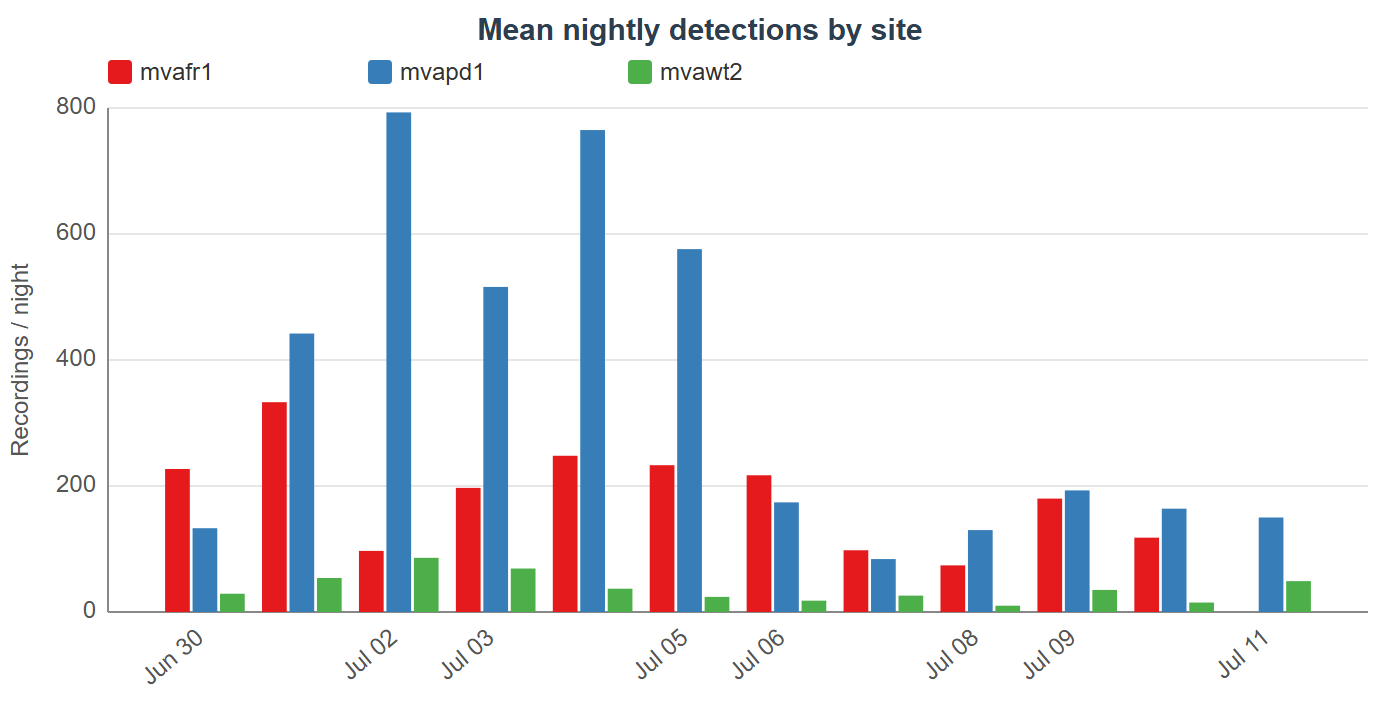
\includegraphics[width=1\linewidth,height=\textheight,keepaspectratio]{Figures/AppendixB/315563_bar.png}

}

\caption{Nightly activity by site (2025 top, 2024 below), cell 315563 -
Valley}

\end{figure}%

\newpage

\begin{figure}[H]

{\centering 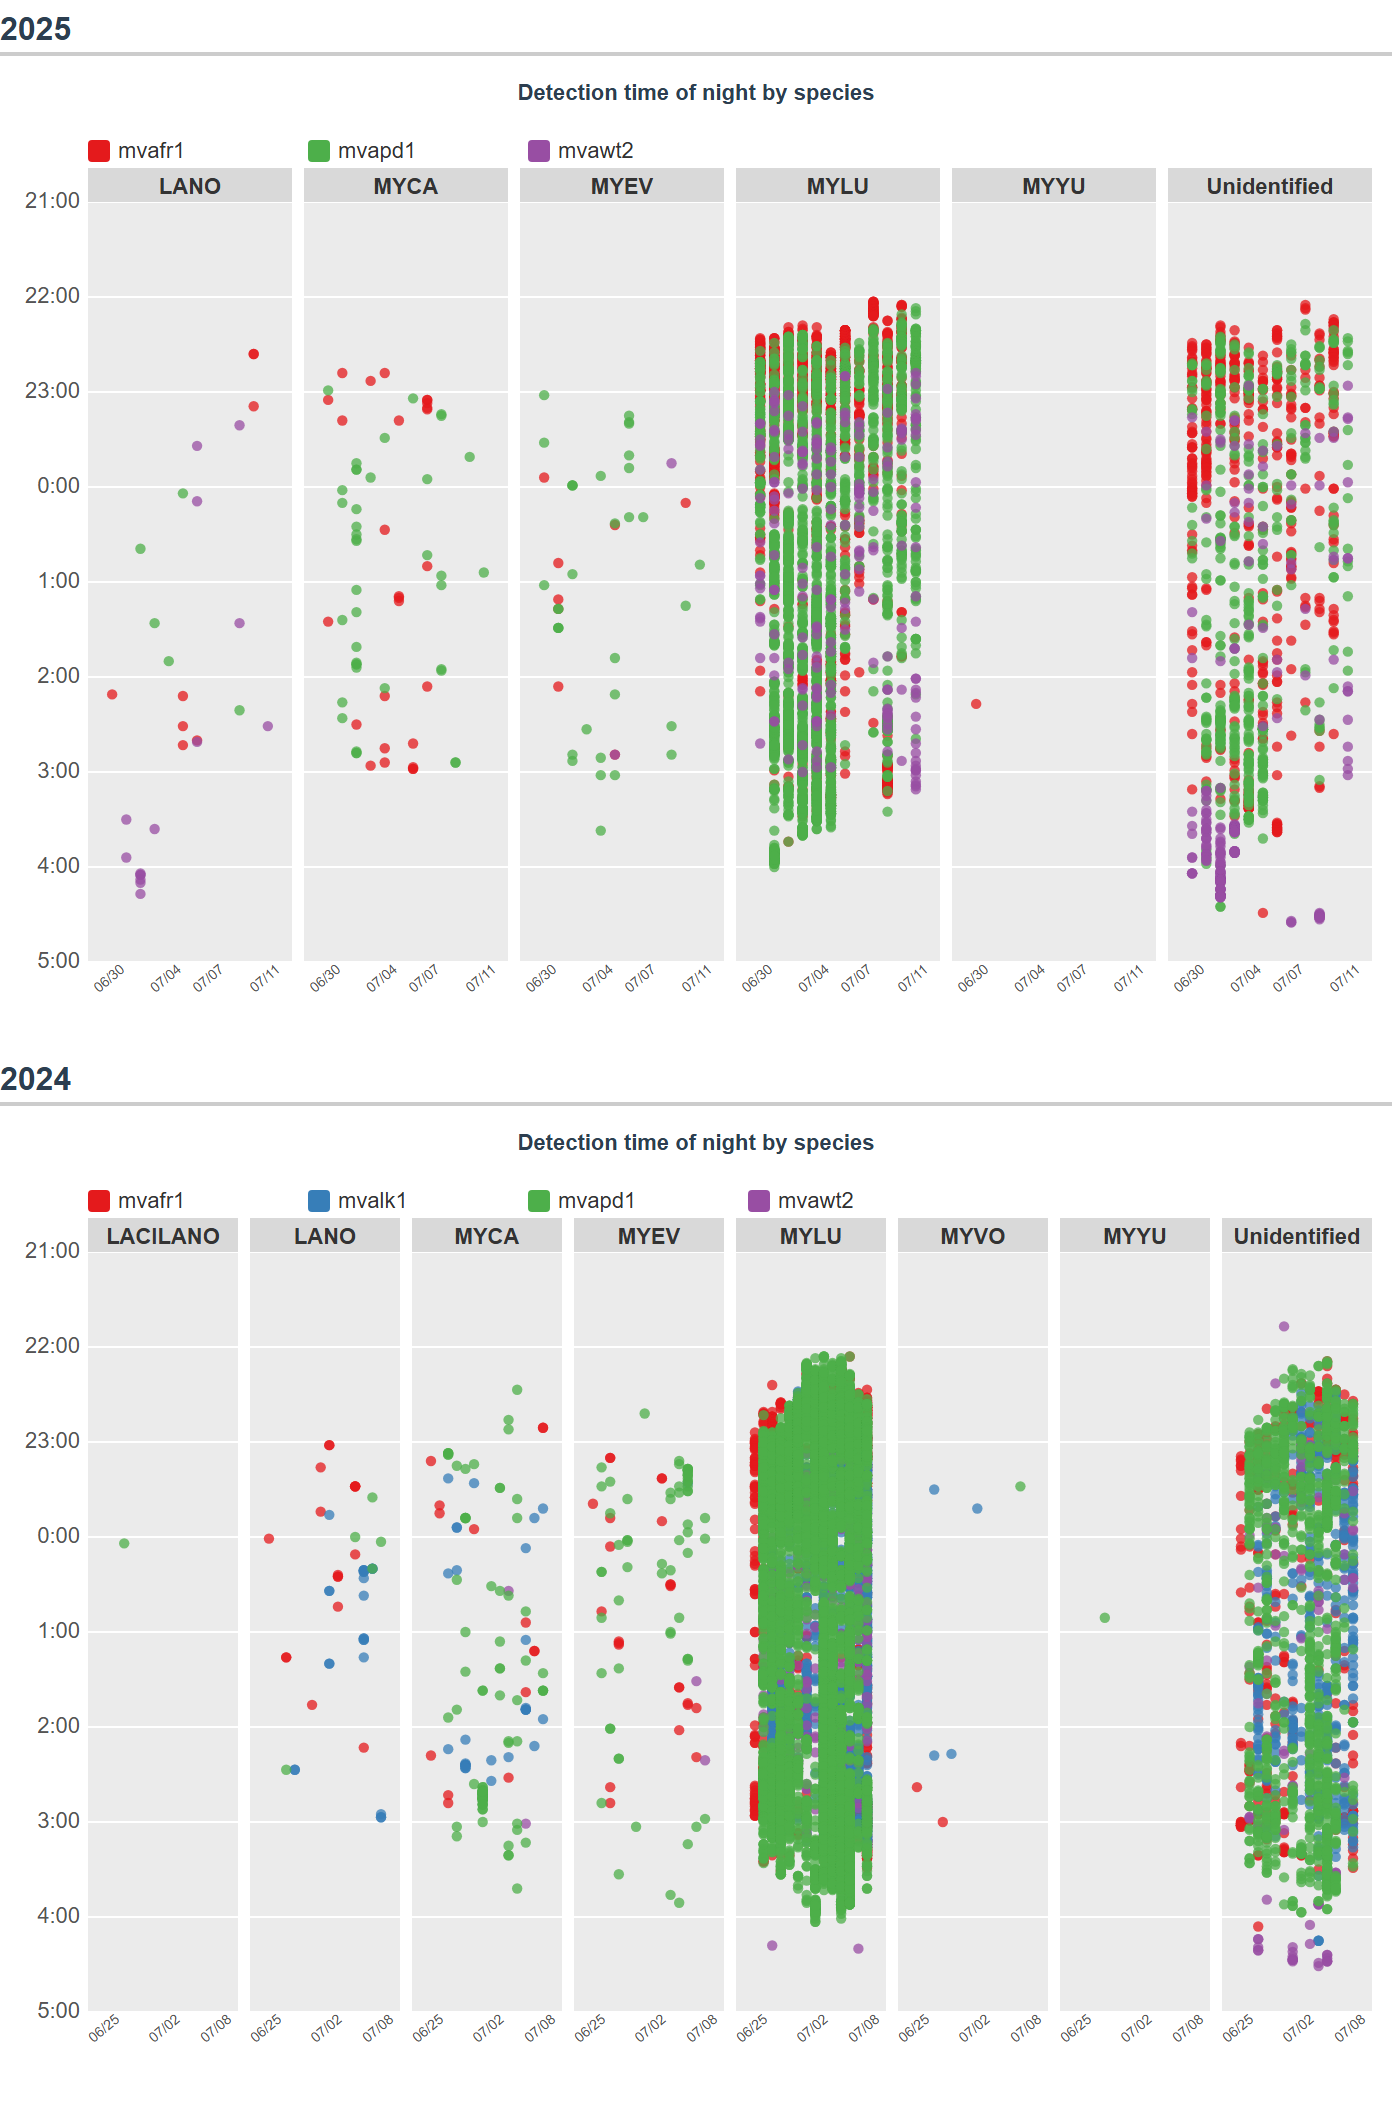
\includegraphics[width=1\linewidth,height=\textheight,keepaspectratio]{Figures/AppendixB/315563_hour.png}

}

\caption{Detection times by species and site (2025 top, 2024 below),
cell 315563 - Valley}

\end{figure}%

\newpage{}

\section*{Literature Cited}\label{literature-cited}
\addcontentsline{toc}{section}{Literature Cited}

\protect\phantomsection\label{refs}
\begin{CSLReferences}{1}{1}
\bibitem[\citeproctext]{ref-blejwas2023}
Blejwas, Karen, Laura Beard, Joseph Buchanan, et al. 2023. {``Could
White-Nose Syndrome Manifest Differently in Myotis Lucifugus in Western
Versus Eastern Regions of North America? A Review of Factors.''}
\emph{Journal of Wildlife Diseases. 59(3): 381{\textendash}397} 59:
381--97. \url{https://doi.org/10.7589/JWD-D-22-00050}.

\bibitem[\citeproctext]{ref-blejwas2021}
Blejwas, Karen, Grey Pendleton, Michael Kohan, and Laura Beard. 2021.
{``The Milieu Souterrain Superficiel as Hibernation Habitat for Bats:
Implications for White-Nose Syndrome.''} \emph{Journal of Mammalogy} 102
(June): 1110--27. \url{https://doi.org/10.1093/jmammal/gyab050}.

\bibitem[\citeproctext]{ref-cheng2021}
Cheng, Tina L., Jonathan D. Reichard, Jeremy T. H. Coleman, et al. 2021.
{``The Scope and Severity of White-Nose Syndrome on Hibernating Bats in
North America.''} \emph{Conservation Biology} 35 (5): 1586--97.
\url{https://doi.org/10.1111/cobi.13739}.

\bibitem[\citeproctext]{ref-loeb2015}
Loeb, Susan C., Thomas J. Rodhouse, Laura E. Ellison, et al. 2015.
\emph{A Plan for the North American Bat Monitoring Program (NABat)}.
Asheville, NC. \url{https://doi.org/10.2737/SRS-GTR-208}.

\bibitem[\citeproctext]{ref-mackenzie2003}
MacKenzie, Darryl I., James D. Nichols, James E. Hines, Melinda G.
Knutson, and Alan B. Franklin. 2003. {``Estimating Site Occupancy,
Colonization, and Local Extinction When a Species Is Detected
Imperfectly.''} \emph{Ecology} 84 (8): 2200--2207.
\url{https://doi.org/10.1890/02-3090}.

\bibitem[\citeproctext]{ref-meteostat}
Meteostat. 2026. \emph{Meteostat: Access and Analyze Historical Weather
and Climate Data with Python}. V. 2.1.4. Released.
\url{https://pypi.org/project/meteostat/}.

\bibitem[\citeproctext]{ref-nasbrst2024}
\emph{NASBR Statement on Wind Energy Impacts on Bat Populations}. 2024.
\url{https://www.nasbr.org/wind}.

\bibitem[\citeproctext]{ref-neubaum2018}
Neubaum, Daniel J. 2018. {``Unsuspected Retreats: Autumn Transitional
Roosts and Presumed Winter Hibernacula of Little Brown Myotis in
Colorado.''} \emph{Journal of Mammalogy} 99 (6): 1294--306.
\url{https://doi.org/10.1093/jmammal/gyy120}.

\bibitem[\citeproctext]{ref-olson2014First}
Olson, Link E., and Aren M. Gunderson. 2014. {``First {Records} of {Yuma
Myotis} ({Myotis} Yumanensis) in {Alaska}.''} \emph{Northwestern
Naturalist} 95 (3): 228--35. \url{https://doi.org/10.1898/13-29.1}.

\bibitem[\citeproctext]{ref-raeBlejwas2026Alaska}
Rae, Jason, and Karen Blejwas. 2026. \emph{North {American Bat
Monitoring Program} in {Alaska}. 2015 - 2023 {Data Summary} and
{Activity Trend Analyses}}. {Wildlife Conservation Society Canada
(WCSC)}.

\bibitem[\citeproctext]{ref-rae2024}
Rae, Jason, and Cori L Lausen. 2024. \emph{North American Bat Monitoring
Program in British Columbia}.

\bibitem[\citeproctext]{ref-reichert2018}
Reichert, Brian, Cori Lausen, Susan Loeb, et al. 2018. \emph{A Guide to
Processing Bat Acoustic Data for the North American Bat Monitoring
Program (NABat)}.

\bibitem[\citeproctext]{ref-segers}
Segers, Jordi. n.d. \emph{CWHC-RCSF :: Canadian Wildlife Health
Cooperative - Réseau Canadien Pour La Santé de La Faune}.
\url{https://www.cwhc-rcsf.ca/white_nose_syndrome_reports_and_maps.php\#top}.

\bibitem[\citeproctext]{ref-segers2025}
Segers, Jordi, Scott McBurney, Megan Jones, and Damien Joly. 2025.
\emph{The Canadian Wildlife Health Cooperative Annual National Bat
Health Report {\textendash} 2025}.

\bibitem[\citeproctext]{ref-stratton2022}
Stratton, Christian, Kathryn M. Irvine, Katharine M. Banner, Wilson J.
Wright, Cori Lausen, and Jason Rae. 2022. {``Coupling Validation Effort
with in Situ Bioacoustic Data Improves Estimating Relative Activity and
Occupancy for Multiple Species with Cross{-}Species
Misclassifications.''} \emph{Methods in Ecology and Evolution} 13 (6):
1288--303. \url{https://doi.org/10.1111/2041-210X.13831}.

\bibitem[\citeproctext]{ref-WNS}
White Nose Syndrome Response Team. 2026. \emph{White-Nose Syndrome}.
\url{https://www.whitenosesyndrome.org/}.

\end{CSLReferences}




\end{document}
